\documentclass{thesisby}

%\usepackage[cp1251]{inputenc}
\usepackage[utf8]{inputenc}
\usepackage[T2A]{fontenc}
\usepackage[russian]{babel}

%\usepackage{pscyr}
%\renewcommand{\rmdefault}{ftm}

%для борьбы с переполнениями за счет разреженных слов в абзаце
\emergencystretch=25pt
%math
\usepackage{mathtools}
\usepackage{tabularx}
\usepackage{pdflscape}

\usepackage{afterpage}
\usepackage{geometry}
\usepackage{multirow}
\usepackage{enumitem}

\usepackage{amsmath,amssymb,amsfonts}
\usepackage{longtable,array}
\usepackage{graphicx,epsfig}
\usepackage[unicode,colorlinks=false,pagebackref=false, hidelinks]{hyperref}
\urlstyle{same}
%\usepackage{refcheck}% checks lost and useless labels, shows `keys' of \label in the margins
%фиксить картинки
%\usepackage{float}

\usepackage{textcomp}% For Celsium sign only

% Листинги с исходным кодом программ
\usepackage{fancyvrb}
\usepackage{listings}
\usepackage{totcount}
%\usepackage{totpages}
\usepackage{cite}

% Плавающие окружения. во многом лучше пакета float
\usepackage{floatrow}

\usepackage{tikz}
\newcolumntype{P}[1]{>{\centering\arraybackslash}p{#1}}
\newcolumntype{M}[1]{>{\centering\arraybackslash}m{#1}}

%for lists
\usepackage[ampersand]{easylist}
\ListProperties(Hide=100, Hang=false, Margin=0mm, Indent1=10.5mm, Indent2=15mm, Style*=-- ,
Style2*=$\bullet$ ,Style3*=$\circ$ ,Style4*=\tiny$\blacksquare$ )

\usepackage[ruled, vlined]{algorithm2e}
\makeatletter
\newenvironment{algo}[1][]
  {\renewcommand{\algorithmcfname}{Алгоритм}%
   \begin{algorithm}[#1]
   \long\def\@caption##1[##2]##3{%
     \par
     \begingroup\@parboxrestore
     \if@minipage\@setminipage\fi
     \normalsize \@makecaption{\AlCapSty{\AlCapFnt\algorithmcfname}}{\ignorespaces ##3}%
     \par\endgroup
   }}
  {\end{algorithm}}
\makeatother

% \SetKwData{KwDat}{Данные}
\SetKwInput{KwIn}{Исходные данные}
\SetKwInput{KwRes}{Результат}%
% \SetKwIF{Si}{SinonSi}{Sinon}{si}{alors}{sinon si}{sinon}{fin si}%
% \SetKwFor{Tq}{tant que}{faire}{fin tq}%

\newenvironment{easylistNum}{\begin{easylist}
\ListProperties(Hide1=0, Hang=false, Margin=0mm, Indent1=10.5mm, Indent2=15mm, Start1=1, Style*=, FinalMark={)})}{\ListProperties(Hide=100, Hang=false, Margin=0mm, Indent1=10.5mm, Indent2=15mm, Style*=-- ,
Style2*=$\bullet$ ,Style3*=$\circ$ ,Style4*=\tiny$\blacksquare$ )\end{easylist}}

\renewcommand\labelitemi{\textbf{--}}
\floatsetup[table]{capposition=top}

    % \lstset{
    %     language=Python,
    %     basicstyle=\ttfamily,
    %     keywordstyle=\bfseries,
    %     showspaces=false,
    %     showstringspaces=false,
    %     mathescape=true,
    %     aboveskip=0pt,
    %     belowskip=6pt
    % }
\lstdefinestyle{PythonStyle}{
  keywordstyle=\bf,
  belowcaptionskip=1\baselineskip,
  breaklines=true,
  language=Python,
  showstringspaces=false,
  basicstyle=\small\ttfamily,
  commentstyle=\itshape
}
% \lstdefinestyle{PythonStyle}{
% basicstyle=\footnotesize\ttfamily,
% language=Python,
% keywordstyle=\bfseries,
% showstringspaces=false,
% commentstyle={},
% texcl=true
% }

\graphicspath{{../}}

%\renewcommand{\cftchapleader}{\cftdotfill{\cftdotsep}}


\begin{document}
\def\contentsname{СОДЕРЖАНИЕ}
\hypersetup{
pdftitle = {МЕТОДЫ ОБУЧЕНИЯ ГЛУБОКИХ НЕЙРОННЫХ СЕТЕЙ ДЛЯ ЗАДАЧ КОМПЬЮТЕРНОГО ЗРЕНИЯ},
pdfauthor = {Крощенко 
Александр Александрович},
pdfsubject = {Диссертация},
pdfkeywords = {ТеХ, диссертация}
}% End of hypersetup

\begin{titlepage}

\begin{center} \bfseries
% Национальная академия наук Беларуси\\
\bigskip
% {Учреждение образования}
\medskip

{УО <<БРЕСТСКИЙ ГОСУДАРСТВЕННЫЙ ТЕХНИЧЕСКИЙ УНИВЕРСИТЕТ>>}
\end{center}
\vspace{1cm}

\noindent УДК 004.032.26 \\
\vspace{1cm}

\begin{center}
{КРОЩЕНКО \\ Александр Александрович}\\ \vspace{1cm}

{\bfseries МЕТОДЫ ОБУЧЕНИЯ ГЛУБОКИХ НЕЙРОННЫХ СЕТЕЙ 
ДЛЯ ЗАДАЧ КОМПЬЮТЕРНОГО ЗРЕНИЯ}\\
\vspace{2cm}
Диссертация на соискание ученой степени\\
кандидата технических наук\\
\bigskip

по специальности 05.13.17 -- Теоретические основы информатики
\end{center}
\vspace{3cm}

\begin{tabbing}
\hspace{8cm} \= \kill \>
Научный руководитель --\+ \\
доктор технических наук, профессор\\
Головко В. А.
\end{tabbing}
\vspace{7cm}

\begin{center}
 \bfseries Брест 2023
\end{center}

\end{titlepage}

\hyphenpenalty=10000
\tableofcontents     % Оглавление
\hyphenpenalty=50

\parindent=1.25cm
%\chapter*{Термины и определения}

%\addcontentsline{toc}{chapter}{Термины и определения}

%В настоящей диссертации применяют
%следующие термины с соответствующими определениями
\chapter*{Перечень сокращений и обозначений}
\addcontentsline{toc}{chapter}{Перечень сокращений и обозначений}
%\sectioncentered*{Перечень условных обозначений}
%\addcontentsline{toc}{section}{Перечень условных обозначений}
%\label{sec:reduction}

\textit{ГНС} -- глубокая нейронная сеть

\textit{ИНС} -- искусственная нейронная сеть

\textit{НС} -- нейронная сеть

\textit{СНС} -- сверточная нейронная сеть

\textit{AP (англ. Average Precision metric)} -- метрика, используемая для оценки методов детекции объектов на изображениях, применяется для одноклассовых случаев

\textit{CD (англ. Contrastive Divergence)} -- контрастное расхождение

\textit{CE (англ. Cross-Entropy error)} -- кросс-энтропийная функция ошибок

\textit{CIFAR (англ. Canadian Institute For Advanced Research)} -- Канадский институт перспективных исследований

\textit{COCO (англ. Common Objects in Context)} -- выборка размеченных изображений, применяемая для решения задач обнаружения, сегментации и аннотирования объектов на изображениях

\textit{C-RBM (англ. Classic Restricted Boltzmann Machine Training)} -- классический метод обучения ограниченной машины Больцмана

\textit{DNN (англ. Deep Neural Network)} -- глубокая нейронная сеть

\textit{IoU (англ. Intersection over Union, мера Жаккара)} -- метрика, применяемая для оценки эквивалентности двух множеств, в задачах компьютерного зрения применяется для оценки методов детекции (обнаружения) объектов как величина, описывающая степень перекрытия двух прямоугольных областей, используемых для определения эталонной и предсказываемой моделью локализации объекта 

\textit{HREBA (англ. Hybrid Reconstruction Error-Based Approach)} -- гибридный вариант предобучения ГНС, сочетающий в себе использование классического (C-RBM) и предлагаемого в данной работе (REBA) методов обучения ограниченной машины Больцмана

\textit{mAP (англ. mean-Average Precision metric)} -- метрика, применяемая для оценки качества алгоритмов детекции объектов на изображениях, применяется для многоклассовых случаев детекции

\textit{MNIST (англ. Mixed National Institute of Standards and Technology database)} -- смешанная база Национального института стандартов и технологии

\textit{MSE (англ. Mean Squared Error)} -- среднеквадратичная ошибка

\textit{Faster-RCNN (англ. Faster Region-based Convolutional Neural Network)} -- архитектура глубокой сверточной нейронной сети, применяемая для решения задачи детекции (обнаружения) объектов на изображениях

\textit{PCA (англ. Principal Component Analysis)} -- метод главных компонент

\textit{RBM (англ. Restricted Boltzmann Machine)} -- ограниченная машина Больцмана

\textit{REBA (англ. Reconstruction Error-Based Approach)} -- метод обучения ограниченной машины Больцмана, базирующийся на минимизации ошибки восстановления образов на видимом и скрытом слоях

\textit{ReLU (англ. Rectified Linear Unit)} -- исправленный линейный элемент

\textit{ResNet-50 (англ. Residual Neural Network)} -- архитектура глубокой нейронной сети, которая характеризуется передачей сигналов между отдельными слоями модели, применяется в качестве классификатора

\textit{SVM (англ. Support Vector Machines)} -- метод опорных векторов

\textit{SVHN (англ. The Street View House Numbers)} -- выборка изображений номеров домов

% ACL (англ. Agent Communication Language) -- язык взаимодействия агентов, предложенный FIPA в качестве стандарта

% FIPA (англ. Foundation for Intelligent Physical Agents) -- организация, осуществляющая разработку и продвижение стандартов в области многоагентных систем

% GPS (англ. General Problem Solver) -- компьютерная программа, созданная в 1959 г. и предназначенная для работы в качестве универсальной машины для решения задач, сформулированных на языке хорновских дизъюнктов

% IACPaaS (англ. Intelligent Applications, Control and Platform as a Service) -- исследовательская облачная платформа, объединяющая различные модели парадигмы облачных вычислений

% IMS (англ. Intelligent MetaSystem) -- интеллектуальная метасистема поддержки проектирования интеллектуальных систем

% KIF (англ. Knowledge Interchange Language) -- компьютерно-ориентированный язык для обмена знаниями между различными компьютерными программами

% KQML (англ. Knowledge Query and Manipulation Language) -- язык взаимодействия между программными агентами и системами, основанными на знаниях

% OSTIS (англ. Open Semantic Technology for Intelligent Systems) -- открытая семантическая технология проектирования интеллектуальных систем

% OWL (англ. Web Ontology Language) -- язык описания онтологий для семантической паутины

% QA3 (англ. Question Answer system ver. 3) -- вопросно-ответная дедуктивная система, созданная в 1969 г. на языке LISP

% RDF (англ. Resource Description Framework) -- разработанная Консорциумом Всемирной паутины модель для представления данных

% SCg-код (англ. Semantic Code graphic) -- графический нелинейный вариант визуализации текстов SC-кода

% SCn-код (англ. Semantic Code natural) -- гипертекстовый вариант визуализации текстов SC-кода

% SCP (англ. Semantic Code Programming) -- графовый процедурный язык программирования, построенный на базе SC-кода

% SC-код (англ. Semantic Code) -- универсальный базовый способ смыслового представления знаний в виде семантических сетей с базовой теоретико-множественной интерпретацией

% SPARQL (англ. SPARQL Protocol and RDF Query Language) -- язык запросов к данным (является рекомендацией консорциума W3C и одной из технологий семантической паутины), представленным по модели RDF, а также протокол для передачи этих запросов и ответов на них

% SQL (англ. Structured Query Language — «язык структурированных запросов») —- универсальный язык запросов, применяемый для создания, модификации и управления данными в реляционных базах данных

% STRIPS (англ. Stanford Research Institute Problem Solver) -- планирующая система, использующая декларативно-процедуральное представление знаний в сочетании с эвристическим поиском, создана в 1971 г.

% W3C (англ. World Wide Web Consortium, W3C) -- Консорциум Всемирной паутины, организация, разрабатывающая и внедряющая технологические стандарты для Всемирной паутины

% ГРЗ -- гибридный решатель задач

% ИСС -- интеллектуальная справочная система

% НИЦ ЭВТ -- московский Научно-исследовательский центр электронной вычислительной техники

% ППР (Программа принятия решений) -- планирующая система для интеллектуального робота, созданная в 1977 г. под руководством В. П. Гладуна

% ПРИЗ (Пакет прикладных инженерных задач) -- система программирования, созданная под руководством Э. Х. Тыугу в 1970--1976 гг

% РЗ -- решатель задач

% УСК -- универсальный семантический код, разработанный В. В. Мартыновым


\chapter*{Введение}
\addcontentsline{toc}{chapter}{Введение}
%{ВВЕДЕНИЕ~.~.~.~.~.~.~.~.~.~.~.~.~.~.~.~.~.~.~.~.~.~.~.~.~.~.~.~.~.~.~.~.~.~.~.~.~.~.~.~.~.~.~.~.~.~.~.~.~.~.}

% В настоящее время все более актуальным становится использование интеллектуальных систем в самых различных областях. Одним из ключевых компонентов интеллектуальной системы, обеспечивающим возможность решать широкий круг задач, является решатель задач. Особенностью решателей задач интеллектуальных систем по сравнению с другими современными программными системами является необходимость решать задачи в условиях, когда сведения, необходимые для решения задачи, не локализованы явно в базе знаний интеллектуальной системы и должны быть найдены в процессе решения задачи на основании каких-либо критериев.

% \ifx\isabstract\undefined 
% Состав решателя задач каждой конкретной системы зависит от ее назначения, классов решаемых задач, предметной области и ряда других факторов.
% \fi

% \ifx\isabstract\undefined 
% В общем случае решатель задач обеспечивает возможность решения задач, связанных как с непосредственно основной функциональностью системы, так и с обеспечением эффективности работы такой системы, а также с обеспечением автоматизации развития самой этой системы. Решатель задач, обеспечивающий выполнение всех перечисленных функций, будем называть \textit{объединенным решателем задач} указанной интеллектуальной системы.
% \fi

% %Ключевой отличительной особенностью решателей задач от современных программных систем вообще является необходимость решать задачи в условиях, когда исходные данные для задачи не локализованы явно
% %Отличительными особенностями решателей задач является их ориентация на обработку знаний, хранящихся в базе знаний интеллектуальной системы, а также 

% Расширение областей применения интеллектуальных систем требует от таких систем возможности решения комплексных задач, решение каждой из которых предполагает совместное использование целого ряда различных моделей представления знаний и различных моделей решения задач. Кроме того, решение комплексных задач предполагает использование общих информационных ресурсов (в предельном случае -- всей базы знаний интеллектуальной системы) различными компонентами решателя, ориентированными на решение различных подзадач. Поскольку решатель комплексных задач осуществляет интеграцию различных моделей решения задач, будем называть его \textit{гибридным решателем задач}.

% Примерами комплексных задач являются:

% \begin{easylist}
% &	задачи понимания текстов естественного языка (как печатных, так и рукописных), понимания речевых сообщений, изображений\ifx\isabstract\undefined. В каждом из перечисленных случаев необходимо осуществить синтаксический анализ обрабатываемого файла (сигнала), устранить незначимые фрагменты, классифицировать значимые фрагменты, соотнести их с понятиями, известными системе, выявить те фрагменты, которые система распознать не в состоянии, устранить дублирование информации и т. д.\fi;
% &	задачи автоматизации адаптивного обучения школьников и студентов\ifx\isabstract\undefined, предполагающие, что система может самостоятельно решать различные задачи из некоторой предметной области, а также управлять процессом обучения, самостоятельно формировать задания для учащихся и контролировать их выполнение\fi;
% &	задачи планирования поведения интеллектуальных роботов\ifx\isabstract\undefined, предполагающие как понимание различного рода внешней информации, так и принятие различных решений с использованием как достоверных методов, так и правдоподобных\fi;
% &	задачи комплексной и гибкой автоматизации различных предприятий;
% &	и другие.
% \end{easylist}

% Использование различных моделей решения задач в рамках
% интеллектуальной системы предполагает декомпозицию комплексной задачи на подзадачи, которые могут быть решены с помощью одной из известных интеллектуальной системе моделей решения задач. Благодаря комбинации различных моделей решения задач, множество задач, решаемых гибридным решателем, будет значительно шире, чем объединение множеств задач, решаемых по отдельности всеми решателями задач, входящими в его состав\ifx\isabstract\undefined ~\cite{Tarasov2007}\fi.

% \ifx\isabstract\undefined
% Значительный вклад в разработку и исследование моделей, методов и средств решения задач в интеллектуальных системах внесли такие ученые, как E. W. Dijkstra, C. A. Hoare, P. Jackson, J. McCarthy, A. Newell, P. Norvig, G. Polya, R. Reiter, S. Russel, H. A. Simon, D. Waterman, M. Wooldridge, А. Н. Аверкин, И. З. Батыршин, А. Н. Борисов, В. Б. Борщев, В. Н. Вагин, Т. А. Гаврилова, Л. А. Гладков, В. А. Головко, А. Н. Горбань, В. И. Городецкий, В. В. Грибова, А. П. Еремеев, Ю. А. Загорулько, А. С. Клещев, А. В. Колесников, В. Е. Котов, О. П. Кузнецов, В. М. Курейчик, Д. В. Ландэ, Л. В. Массель, А. С. Нариньяни, Г. С. Осипов, Г. С. Плесневич, Э. В. Попов, Д. А. Поспелов, Г. В. Рыбина, П. О. Скобелев, В. Б. Тарасов, Э. Х. Тыугу, В. К. Финн, И. Б. Фоминых, В. Ф. Хорошевский, А. Е. Янковская и др.
% \fi

% Постоянная эволюция интеллектуальных систем и технологий их разработки делает актуальной не только проблему снижения сроков разработки гибридных решателей задач, но и проблему снижения трудоемкости внесения изменений в состав уже разработанных решателей без необходимости изменения архитектуры всей системы в целом. 

% Современные подходы к построению гибридных решателей задач, как правило, предполагают совмещение разнородных моделей решения задач без какой-либо единой основы, например, посредством специализированных программных интерфейсов между разными компонентами системы, что приводит к существенным накладным расходам при разработке такой системы и в особенности при ее модификации, в том числе при добавлении в систему новой модели решения задач. 

% Таким образом, несмотря на успехи в области разработки решателей задач интеллектуальных систем, остаются нерешенными проблемы, связанные с обеспечением:
% \begin{easylist}
% & совместимости различных частных решателей задач, т. е. возможности их согласованного использования при решении одной и той же комплексной задачи;
% & возможности без существенных накладных расходов модифицировать гибридный решатель непосредственно в процессе эксплуатации интеллектуальной системы, в том числе расширять число используемых моделей решения задач без каких-либо ограничений на вид этих моделей. Такое требование обусловлено тем, что при решении комплексной задачи априори может оказаться неизвестным, какие именно модели решения задач и виды знаний могут потребоваться.
% \end{easylist}

% Важным способом снижения трудоемкости процесса изменения функциональности интеллектуальных систем является накопление библиотек совместимых компонентов решателей, которые позволят значительно снизить как сроки разработки и модификации решателей, так и уровень профессиональных требований к их разработчикам.

% Кроме того, актуальной является проблема создания самих средств разработки гибридных решателей задач, обеспечивающих информационную поддержку и автоматизацию деятельности разработчиков.

Практические приложения компьютерного зрения с каждым годом становятся все более разнообразными. В современном мире компьютерное зрение используется повсеместно -- в сложных производственных и медицинских системах, в интеллектуальных системах интернета вещей и развлекательных приложениях для мобильных устройств.

В качестве основы при разработке таких систем все чаще находят применение глубокие нейросетевые модели. Данные модели показывают впечатляющие результаты при решении самых разнообразных задач компьютерного зрения -- распознавания, детекции и сегментации объектов на фото- и видеоизображениях, получения аннотаций для фотографий и генерации изображений по текстовому описанию. Глубокие нейронные сети, применяемые для решения подобных задач, содержат миллионы настраиваемых параметров и, для некоторых архитектур, десятки слоев нейронных элементов.

Обучение подобных <<тяжелых>> моделей с нуля является нетривиальной задачей. Оно часто сопряжено с риском переобучения, результатом которого является отличная приспособленность сети к данным из обучающей выборки, но плохая обобщающая способность, то есть неэффективность модели для данных, не использовавшихся при обучении. Чаще всего переобученность возникает при применении малой обучающей выборки. Другой проблемой является ресурсоемкость процесса обучения таких моделей, даже при использовании современных технических средств.

Проблемы обучения глубоких нейронных сетей активно изучаются в зарубежных научных школах. В нашей стране такие исследования также проводятся. Однако, нужно отметить, что такие исследования часто носят эмпирический характер, поэтому разработка строгих математически обоснованных методов обучения остается важной задачей теории нейронных сетей.

В диссертационной работе разработаны подходы для неконтролируемого предобучения глубоких нейронных сетей и редуцирования параметров моделей. Предложены алгоритмы для решения практических задач теории компьютерного зрения -- обнаружения и локализации солнечных панелей на аэрофотоснимках, обнаружения и распознавания маркировки на поточных производственных линиях. Предложенные методы и алгоритмы позволят улучшить работу интеллектуальных систем, использующих полносвязные и сверточные нейросетевые модели.


\chapter*{Общая характеристика работы}					
	% Заголовок
\addcontentsline{toc}{chapter}{Общая характеристика работы}	% Добавляем его в оглавление

\newcommand{\actuality}{\textbf{Связь работы с научными программами (проектами), темами}}
\newcommand{\aim}{\textbf{Цель, задачи, объект и предмет исследования}}
%\newcommand{\tasks}{\textit{задачи исследования}}
\newcommand{\novelty}{\textbf{Научная новизна}}
\newcommand{\defpositions}{\textbf{Положения, выносимые на защиту}}
\newcommand{\influence}{\textbf{Научная и практическая значимость}}
\newcommand{\reliability}{\textbf{Степень достоверности}}
\newcommand{\contribution}{\textbf{Личный вклад соискателя ученой степени в результаты диссертации}}
\newcommand{\probation}{\textbf{Апробация диссертации и информация об использовании ее результатов}}
\newcommand{\publications}{\textbf{Опубликованность результатов диссертации}}

{\actuality}
\vspace{3mm}

Тема диссертации соответствует приоритетному направлению научно-технической деятельности согласно пункту 1 перечня приоритетных направлений научной, научно-технической и инновационной деятельности на 2021-2025 годы  (Указ Президента Республики Беларусь от 07 мая 2020 г. № 156).

Исследования по теме диссертационной работы проводились в рамках научных программ:
\begin{enumerate}[wide, labelindent=10mm]
\item НИР МОРБ <<Алгоритмы интеллектуального анализа и обработки больших объемов данных на основе нейронных сетей глубокого доверия>> (ГБ 15/203, № госрегистрации 20150743),
\item ГПНИ <<Информатика и космос, научное обеспечение безопасности и защиты от чрезвычайных ситуаций>> по заданию <<Нейросетевые методы обработки комплексной информации и принятия решений на основе интеллектуальных многоагентных систем>> (№ госрегистрации 20140547),
\item ГПНИ <<Информатика и космос, научное обеспечение безопасности и защиты от чрезвычайных ситуаций>> по заданию <<Методы и алгоритмы интеллектуальной обработки и анализа большого объема данных на основе нейронных сетей глубокого доверия>> (задание 1.6.05, № госрегистрации 20163595),
\item НИР <<Методы и алгоритмы построения интеллектуальных систем анализа и обработки данных>>, этап <<Разработка гибридных интеллектуальных систем на основе нейросимволического подхода>>,
\item НИР БРФФИ <<Модели и исследование 3-D оцифровки на основе фактических данных и анализа гетерогенных данных>> (№ Ф22КИ-046 от 05.11.2021 г., № госрегистрации 20220090).
\end{enumerate}

% Тема диссертации соответствует приоритетному направлению <<Информатика и космические исследования>> согласно пункту 5 перечня приоритетных направлений научных исследований Республики Беларусь на 2016–2020 гг. (Постановление Совета Министров Республики Беларусь от 12 марта 2015 г. № 190).

% Диссертационное исследование выполнено в рамках следующих НИР: <<Семантическая технология компонентного проектирования интеллектуальных решателей задач>> (грант Министерства образования № 12-3134 от 27.12.2011, № ГР 20121587); <<Методы и средства онтологического моделирования для семантических технологий проектирования интеллектуальных систем>> (БРФФИ № Ф15РМ-074 от 04.05.2015 г., № ГР 20151081); <<Формализация темпоральных рассуждений в интеллектуальных системах>> (\mbox{БРФФИ № Ф16Р-102} от 20.05.2016 г., № ГР 20164340); <<Разработка методов и средств поддержки принятия решений при выявлении информационных операций>> (БРФФИ № Ф16К-068 от 21.10.2016 г., № ГР 20164717).

\vspace{3mm}
\aim
\vspace{3mm}

\textit{Целью исследования} является разработка эффективных методов и алгоритмов для обучения глубоких нейронных сетей, используемых для решения задач компьютерного зрения, включающих распознавание маркировки продукта на конвейерной линии и обнаружение солнечных панелей на аэрофотоснимках.

Указанная цель определяет следующие \textit{задачи исследования}:
\begin{easylistNum}
	& Разработать метод неконтролируемого предобучения глубоких нейронных сетей, позволяющий повысить эффективность обучения моделей;
	& Разработать алгоритм редуцирования параметров глубоких нейронных сетей, позволяющий упростить структуру моделей;
	& Провести сравнительный анализ эффективности разработанных метода обучения и алгоритма редуцирования;
	& Разработать нейросетевые системы распознавания маркировки продукта на конвейерной линии и обнаружения солнечных панелей на аэрофотоснимках.
\end{easylistNum}

% \textit{Целью исследования} является разработка комплекса моделей, методики и средств построения и модификации гибридных решателей задач интеллектуальных систем.

% Указанная цель определяет следующие {\tasks}:
% \begin{enumerate}[wide, labelindent=10mm]
%   \item	Проанализировать существующие модели, методики и средства построения решателей задач, а также модели, методы и средства повышения эффективности и модифицируемости таких решателей, в частности, в направлении расширения множества решаемых ими задач.
%   \item	Разработать агентно-ориентированную модель гибридного решателя задач, обеспечивающую интеграцию различных моделей решения задач в рамках одной интеллектуальной системы при решении комплексных задач.
%   \item	Разработать формальную модель взаимодействия информационных процессов в общей семантической памяти, включающую классификацию таких процессов, средства их синхронизации, а также принципы взаимодействия агентов, выполняющих указанные процессы.
%   \item Разработать методику построения и модификации гибридных решателей задач, ориентированных на решение задач в семантической памяти, в основе которой лежит формальное описание деятельности разработчиков таких решателей.
%   \item Разработать средства автоматизации и информационной поддержки процесса построения и модификации решателей задач.
% \end{enumerate}

\textit{Объектом исследования} являются нейросетевые системы компьютерного зрения. \textit{Предметом исследования} выступают методы и алгоритмы обучения глубоких нейронных сетей и их применение к задачам компьютерного зрения.

\vspace{3mm}
\novelty
\vspace{3mm}

Научная новизна состоит в выявлении и доказательстве эквивалентности максимизации функции правдоподобия распределения входных данных, минимизации кросс-энтропийной функции ошибки и суммарной квадратичной ошибки при использовании линейных нейронов в пространстве синаптических связей ограниченной машины Больцмана.

Разработан метод обучения ограниченной машины Больцмана на основе доказанных эквивалентностей, применение которого для предобучения ГНС позволяет расширить класс обучаемых моделей и повысить обобщающую способность ГНС.

Разработан алгоритм редуцирования параметров нейросетевой модели, основывающийся на неконтролируемом предобучении, что позволяет уменьшить количество настраиваемых параметров модели без потери обобщающей способности.

Разработаны нейросетевые системы компьютерного зрения (система распознавания маркировки на производственной линии, система обнаружения солнечных панелей на аэрофотоснимках), которые основываются на применении предложенного метода для выполнения предобучения соответствующих нейросетевых моделей.

\vspace{3mm}
\defpositions
\vspace{3mm}

\begin{enumerate}[wide, labelindent=10mm]
\item Метод обучения ограниченной машины Больцмана, базирующийся на эквивалентности максимизации функции правдоподобия распределения входных данных в пространстве синаптических связей и минимизации суммарной квадратичной ошибки сети при использовании линейных нейронов, что позволяет расширить класс обучаемых моделей и повысить обобщающую способность глубоких нейронных сетей.
\item Алгоритм редуцирования параметров глубокой нейронной сети, базирующийся на неконтролируемом предобучении сети, что позволяет упростить ее архитектуру (путем сокращения числа настраиваемых параметров модели) без потери обобщающей способности.
\item Нейросетевые системы компьютерного зрения, базирующиеся на использовании предобученных моделей -- система распознавания (в реальном режиме времени) маркировки продукта на производственной линии и система обнаружения солнечных панелей на аэрофотоснимках (включая снимки низкого разрешения) с точностью до 87,46\%.

% \item Агентно-ориентированная модель гибридного решателя задач, рассматривающая каждый такой решатель как иерархическую систему агентов, управляемых ситуациями и событиями в общей семантической памяти, обеспечивающая модифицируемость таких решателей задач, а также возможность решения задач, требующих совместного использования различных методов решения задач.
% \item Формальная модель взаимодействия параллельных асинхронных информационных процессов в общей семантической памяти, определяющая принцип коммуникации агентов, выполняющих указанные процессы, включающая средства синхронизации процессов на основе механизма блокировок элементов семантической памяти и обеспечивающая возможность спецификации планируемых блокировок, а также выявления и устранения взаимоблокировок.
% \item Методика построения и модификации гибридных решателей задач, основанная на формальной онтологии деятельности разработчиков таких решателей и ориентированная на применение многократно используемых компонентов решателей, позволяющая снизить сроки разработки решателей как минимум на 31~\% за счет использования разработанных ранее компонентов.
% \item Средства автоматизации и информационной поддержки процесса построения и модификации гибридных решателей задач, включающие средства автоматизации процесса построения агентов обработки знаний и библиотеку многократно используемых компонентов таких решателей, которая в текущий момент позволяет сократить число агентов, разрабатываемых для каждого решателя, как минимум на 37~\%.
\end{enumerate}

%Личный вклад
\vspace{3mm}
\contribution
\vspace{3mm}

Основные положения диссертации получены автором лично. Из публикаций, сделанных в соавторстве, в содержание диссертации включены только те результаты, которые были получены лично соискателем. Соавтором основных публикаций автора является научный руководитель д.т.н., профессор В.А. Головко, который осуществлял определение целей и постановку задач исследований, выбор методов исследований, принимал участие в планировании работ и обсуждении результатов. 

\vspace{3mm}
\probation
\vspace{3mm}

Основные положения и результаты диссертационной работы докладывались и обсуждались на следующих международных конференциях: <<International Conference on Neural Networks and Artificial Intelligence>> (Брест, 2014); <<Информационное, программное и техническое обеспечение систем управления организационно-технологическими комплексами>> (Луцк, 2015); <<8th IEEE International Conference on Intelligent Data Acquisition and Advanced Computing Systems: Technology and Applications>> (Варшава, 2015); <<International Scientific-Practical Conference Problems of Infocommunications. Science and Technology (PIC S\&T)>> (2018); <<International Conference on Pattern Recognition and Information Processing (PRIP)>> (2019); <<Вычислительные методы, модели и образовательные технологии>> (Брест, 2013, 2014, 2015, 2016, 2019); <<Современные проблемы математики и вычислительной техники>> (Брест, 2015); <<Открытые семантические технологии проектирования интеллектуальных систем>> (Минск, 2018, 2019, 2020, 2021, 2023); <<11th IEEE International Conference on Intelligent Data Acquisition and Advanced Computing Systems: Technology and Applications (IDAACS)>> (Краков, 2021).

%Научная и практическая значимость
%\influence\ \ldots

%Степень достоверности
%\reliability\ полученных результатов обеспечивается \ldots \ Результаты находятся в соответствии с результатами, полученными другими авторами.

%Публикации
\vspace{3mm}
\publications
\vspace{3mm}

По теме диссертационной работы опубликовано 28 печатных работ (\textbf{9,48} авторских листа). Из них 11 статей в научных журналах (5,35 авторских листа), 5 статей в сборниках материалов научных конференций, включенных в системы международного цитирования (Scopus, Web of Science и IEEE Xplore digital, 0,48 авторских листа) и 12 статей в сборниках материалов научных конференций (\textbf{3,65} авторских листа).

% По материалам выполненных исследований опубликовано 37 научных ра-
% бот, в том числе 7 статей в рецензируемых изданиях. Без соавторства опубликовано 10 работ, из них 1 статья в рецензируемых изданиях.
% Общий объем публикаций по теме диссертации, соответствующий пункту
% 18 Положения о присуждении ученых степеней и присвоении ученых званий
% в Республике Беларусь, составляет около 18,88 авторского листа.

%По материалам диссертационного исследования опубликовано 37 научных работ, в том числе 7 статей в рецензируемых научных изданиях, соответствующих пункту 18 Положения о присуждении ученых степеней и присвоении ученых званий в Республике Беларусь, общим объемом около 3,5 авт. листа, 3 статьи в научных журналах, 27 статей в материалах республиканских и международных конференций. Без соавторства опубликовано 10 работ, из них 1 статья в рецензируемых изданиях. % Характеристика работы по структуре во введении и в автореферате не отличается (ГОСТ Р 7.0.11, пункты 5.3.1 и 9.2.1), потому её загружаем из одного и того же внешнего файла, предварительно задав форму выделения некоторым параметрам
%% регистрируем счётчики в системе totcounter
% \regtotcounter{totalcount@figure}
% \regtotcounter{totalcount@table}       % Если поставить в преамбуле то ошибка в числе таблиц
% \regtotcounter{TotPages}               % Если поставить в преамбуле то ошибка в числе страниц

%\regtotcounter{page}
%\newtotcounter{mainpage}

% \addtocounter{page}{-1}
%\addtocounter{mainpage}{-1}

\vspace{3mm}
\textbf{Структура и объем диссертации} 
\vspace{3mm}

Диссертация состоит из перечня сокращений и обозначений, введения, общей характеристики работы, четырех глав, заключения, списка использованных источников и двух приложений.

%В \textbf{\textit{первой главе}} рассмотрено краткое введение в теорию искусственных нейронных сетей, дана классификация их типов. Определено понятие глубокой нейронной сети. Рассмотрены задачи обучения глубоких нейронных сетей и существующие методы обучения. \textbf{\textit{Вторая глава}} посвящена рассмотрению разработанного метода обучения ограниченной машины Больцмана и метода предобучения глубоких нейронных сетей на его основе. Также в этой главе предлагается алгоритм редуцирования параметров нейросетевых моделей. В \textbf{\textit{третьей главе}} приведены экспериментальные результаты, обосновывающие полученные теоретические результаты. В \textbf{\textit{четвертой главе}} рассмотрено практическое применение разработанных методов в интеллектуальных системах компьютерного зрения.

Полный объем диссертации составляет 117 страниц, из которых 44 рисунка на 32 страницах, 17 таблиц на 9 страницах, 2 приложения на 14 страницах. Список использованных источников состоит из 121 наименований, включая 30 публикаций автора.

% Диссертация состоит из введения, общей характеристики работы, четырех глав с краткими выводами по каждой главе, заключения, библиографического списка, списка публикаций автора и 17 приложений. Общий объём диссертации составляет 254 страницы, из которых 157 страниц основного текста, 51 рисунок на 26 страницах, 5 таблиц на 4 страницах, библиография из 167 источников, включая 37 публикаций автора, приложения на 50 страницах.
%\total{page} 
%\total{mainpage}

%\textcolor{red}{
%Диссертация состоит из введения, общей характеристики работы, четырех глав с краткими выводами по каждой главе, заключения, библиографического списка, списка публикаций автора и 11 приложений. Общий объём диссертации составляет \formbytotal{TotPages}{страниц}{у}{ы}{}, из которых 171 страниц основного текста, \formbytotal{totalcount@figure}{рисунк}{ом}{ами}{ами}, \formbytotal{totalcount@table}{таблиц}{ей}{ами}{ами}, библиография из 174 источников, включая 56 публикаций автора, приложения на 37 страницах.}

%\textcolor{red}{
%Диссертация состоит из введения, общей характеристики работы, четырех глав с краткими выводами по каждой главе, заключения, библиографического списка, списка публикаций автора и 7 приложений. В первой главе проведен анализ моделей, средств разработки баз знаний и методов их создания. Во второй главе предложена семантическая модель базы знаний. Третья глава содержит описание унифицированной семантической модели процесса создания баз знаний, а также унифицированной семантической модели средств автоматизации процесса создания баз знаний, включая унифицированную семантическую модель библиотеки многократно используемых компонентов баз знаний. В четвертой главе описана реализация разработанных моделей и средств, проведена их оценка.
%% на случай ошибок оставляю исходный кусок на месте, закомментированным
% Полный объём диссертации составляет  \ref*{TotPages}~страницу с~\totalfigures{totalcount@figure}~рисунками и~\totaltables{}~таблицами. Список литературы содержит \total{citenum}~наименований.}

%
%\textcolor{red}{
%Полный объём диссертации составляет
%\formbytotal{TotPages}{страниц}{у}{ы}{} 
%с~\formbytotal{totalcount@figure}{рисунк}{ом}{ами}{ами}
%и~\formbytotal{totalcount@table}{таблиц}{ей}{ами}{ами}. Список литературы %содержит  
%\formbytotal{citenum}{наименован}{ие}{ия}{ий}.}
\chapter{Проблемы обучения глубоких нейронных сетей}

В данной главе вводится теоретическая основа для понимания основных концепций теории обучения глубоких нейронных сетей. Приводится классификация основных типов слоев и архитектур моделей. Описывается историческая ретроспектива развития теории обучения глубоких моделей, а также основные проблемы, которые возникали и возникают при выполнении обучения. 

Осуществляется обзор существующих подходов для обучения глубоких нейронных сетей. Приводится описание методов обучения с использованием стохастического градиентого спуска и функций активации ReLU с ее вариантами. Описываются основные проблемы, присущие подобному типу обучения.

Особое внимание уделяется методам неконтролируемого предобучения, для реализации которых не требуется наличие обучающей выборки большого размера. Главной целью, достигаемой при выполнении предобучения, является формирование <<хорошей>> начальной инициализации параметров глубокой нейронной сети. Подобная инициализация гарантирует сходимость нейросетевой модели в процессе дальнейшего дообучения на этапе <<тонкой настройки>>.

%В контексте проблемы обучения ГНС приводится вывод классических правил обучения ограниченной машины Больцмана (restricted Boltzmann Machine), применяемой на этапе неконтролируемого предобучения ГНС. 

Приводятся алгоритмы предобучения с использованием RBM и автоэнкодерных моделей, формируемых из слоев ГНC и описывается этап <<тонкой настройки>> нейронной сети, цель которого состоит в дообучении модели для решения определенной задачи.

\section{Общие сведения}

Вопросы разработки и применения нейросетевых моделей часто рассматриваются в контексте более широкой области машинного обучения, являющейся по сути одним из направлений современной науки об искусственном интеллекте. При этом само машинное обучение сформировалось на стыке нескольких научных дисциплин, включающих вычислительную математику, теорию вероятностей и статистику, линейную алгебру и теорию оптимизации. С помощью алгоритмов машинного обучения создаются модели, которые используют предшествующий опыт для повышения эффективности компьютера в решении определенных классов задач \cite{mitchell1997machine}. Под понятием предшествующего опыта здесь понимается совокупность статистических данных, собранных при наблюдении и описании некоторого процесса. 

Являясь моделями машинного обучения, нейронные сети также способны к решению различных типов задач после реализации итеративного алгоритма настройки параметров, называемого обучением. Само свойство обучаемости приближает искусственные нейросети к их естественному прототипу, а именно к человеческому мозгу, где обучение является важным процессом в формировании психики \cite{kandel}.
%Являясь одним из методов машинного обучения, нейронные сети Таким образом, алгоритмом машинного обучения можно называть алгоритм, способный обучаться на данных. Фактически являясь одним из алгоритмов машинного обучения, нейронные сети обладают вышеназванным свойством.

В основе теории искусственных нейронных сетей лежит биологически инспирированная модель искусственного нейрона, представляющая собой вычислительный элемент, выполняющий преобразование входных данных (рисунок \ref{fig:pic0_1}). Данное преобразование заключается в вычислении некоторой функции активации (линейной или нелинейной) $F$ от взвешенной суммы $S$ компонент вектора входных данных $X = (x_1, x_2, ..., x_n)$. Параметры $W = (w_1, w_2, ..., w_n)$ называются весовыми коэффициентами (весами) нейрона и настраиваются в процессе обучения в соответствии с определенным правилом обучения. Помимо весовых коэффициентов, у нейрона может быть дополнительный параметр $T$, называемый порогом (или пороговым коэффициентом). Он определяет смещение взвешенной суммы $S$.

\begin{figure}[H]
  \centering
  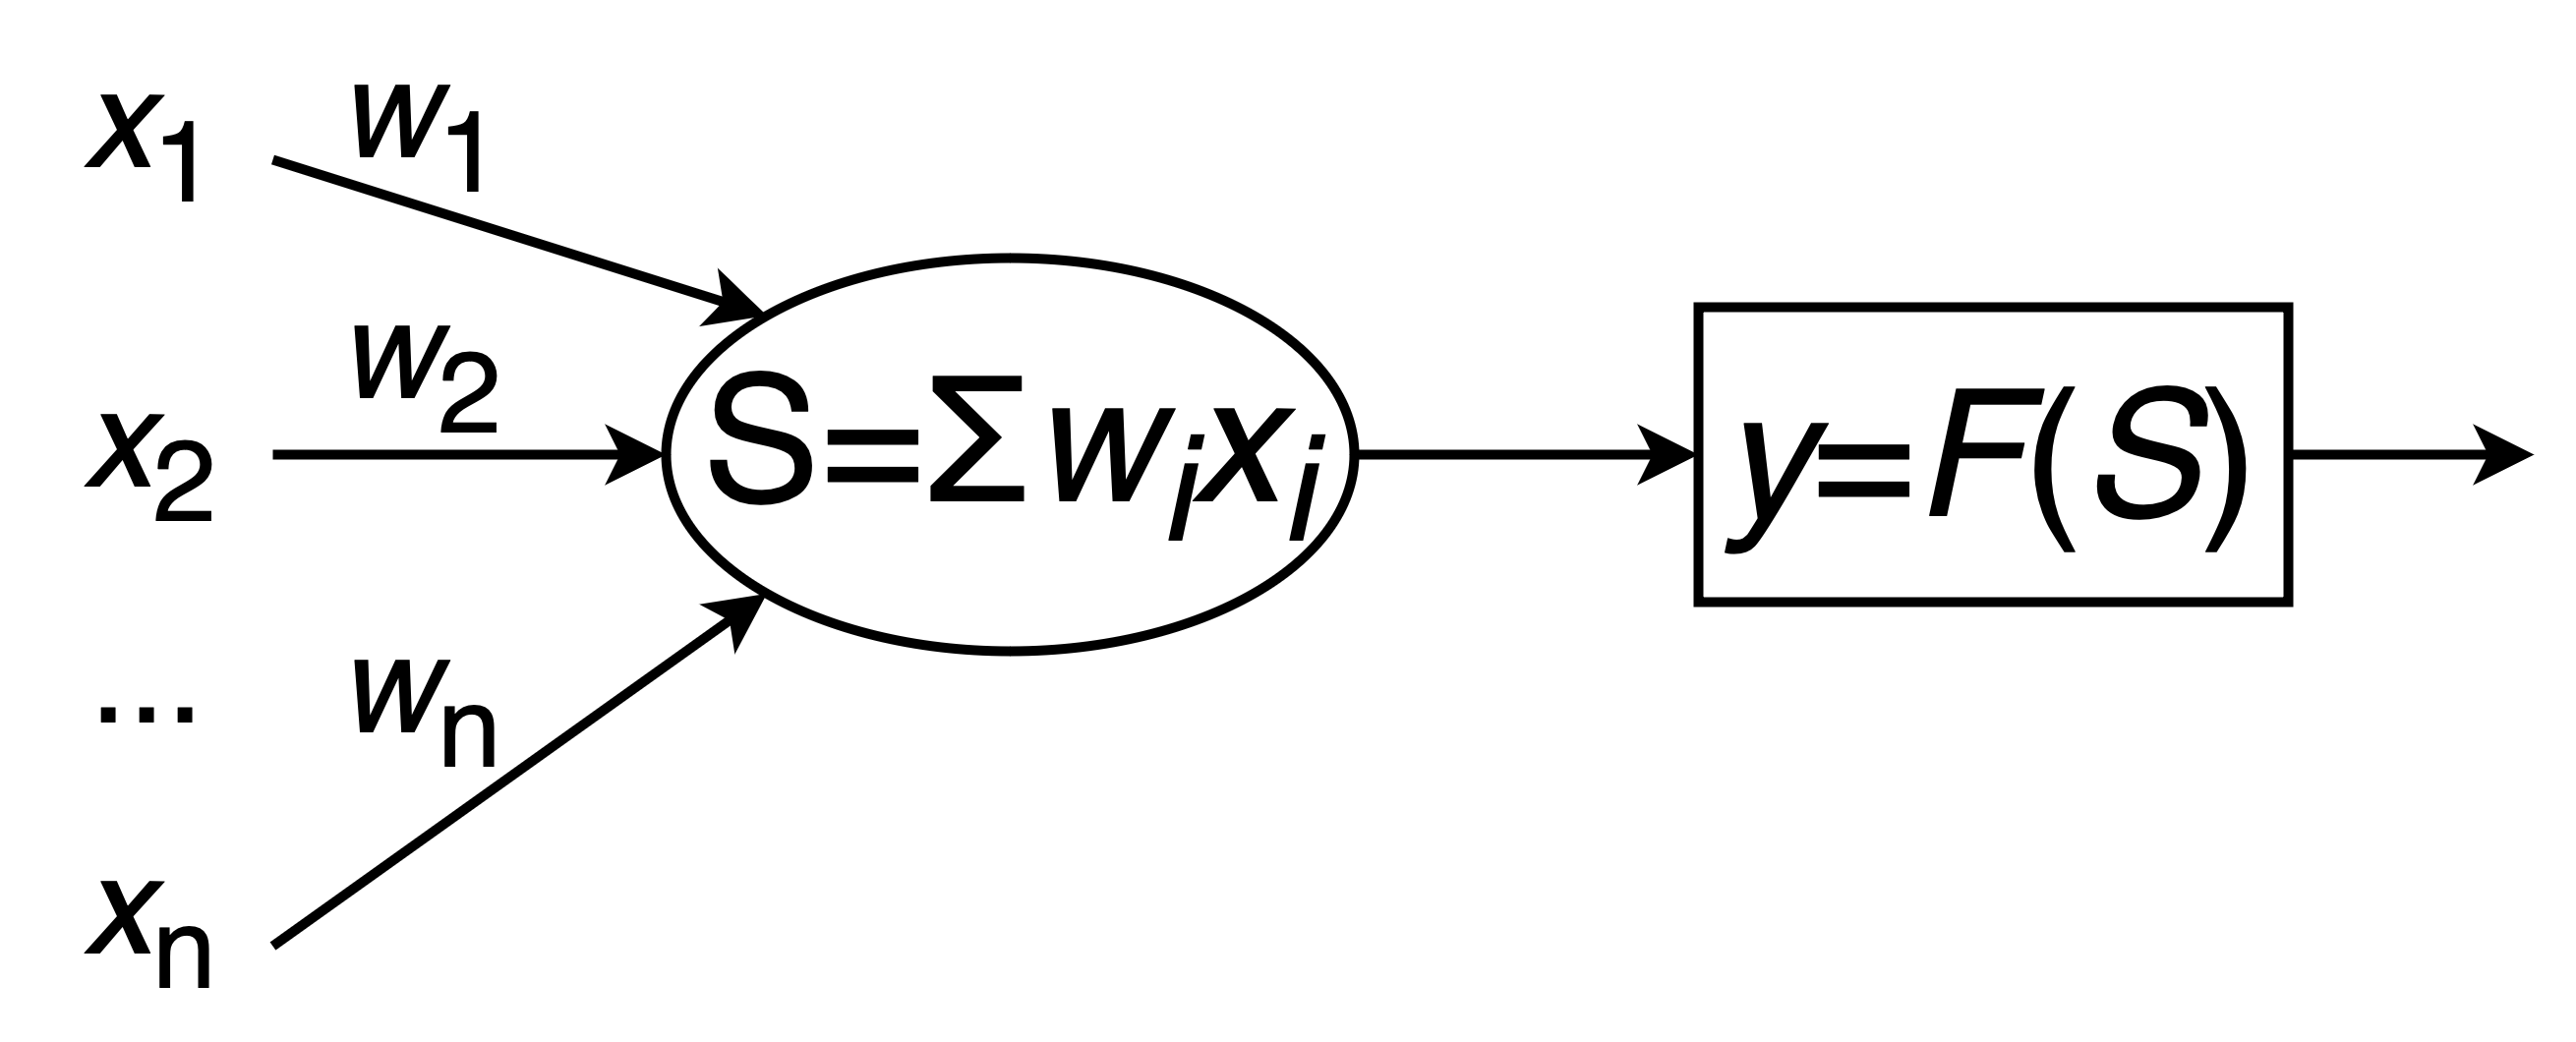
\includegraphics[width=\textwidth]{man-source/images/ch1/pic0-1.png}
  \caption{Модель искусственного нейрона}
  \label{fig:pic0_1}
\end{figure}

Искусственные нейроны могут быть объединены в группы, называемые слоями, по аналогии с биологическими нейронными слоями. Каждый нейрон слоя, обладая независимым набором весовых коэффициентов, получает на вход одинаковый вектор данных $X$ и выполняет его преобразование, формируя отдельную компоненту выходного вектора $Y$, называемого паттерном выходной активности слоя \cite{golovko2017} (рисунок \ref{fig:pic0_2}). Весовые коэффициенты отдельных нейронов для удобства объединяются в матрицу, которая называется матрицей весовых коэффициентов слоя (или матрицей весов). Слой, имеющий настраиваемые параметры, называется обрабатывающим (в отличие от распределительных слоев, которые являются предваряющими в любой НС и не имеют параметров).

\begin{figure}[H]
  \centering
  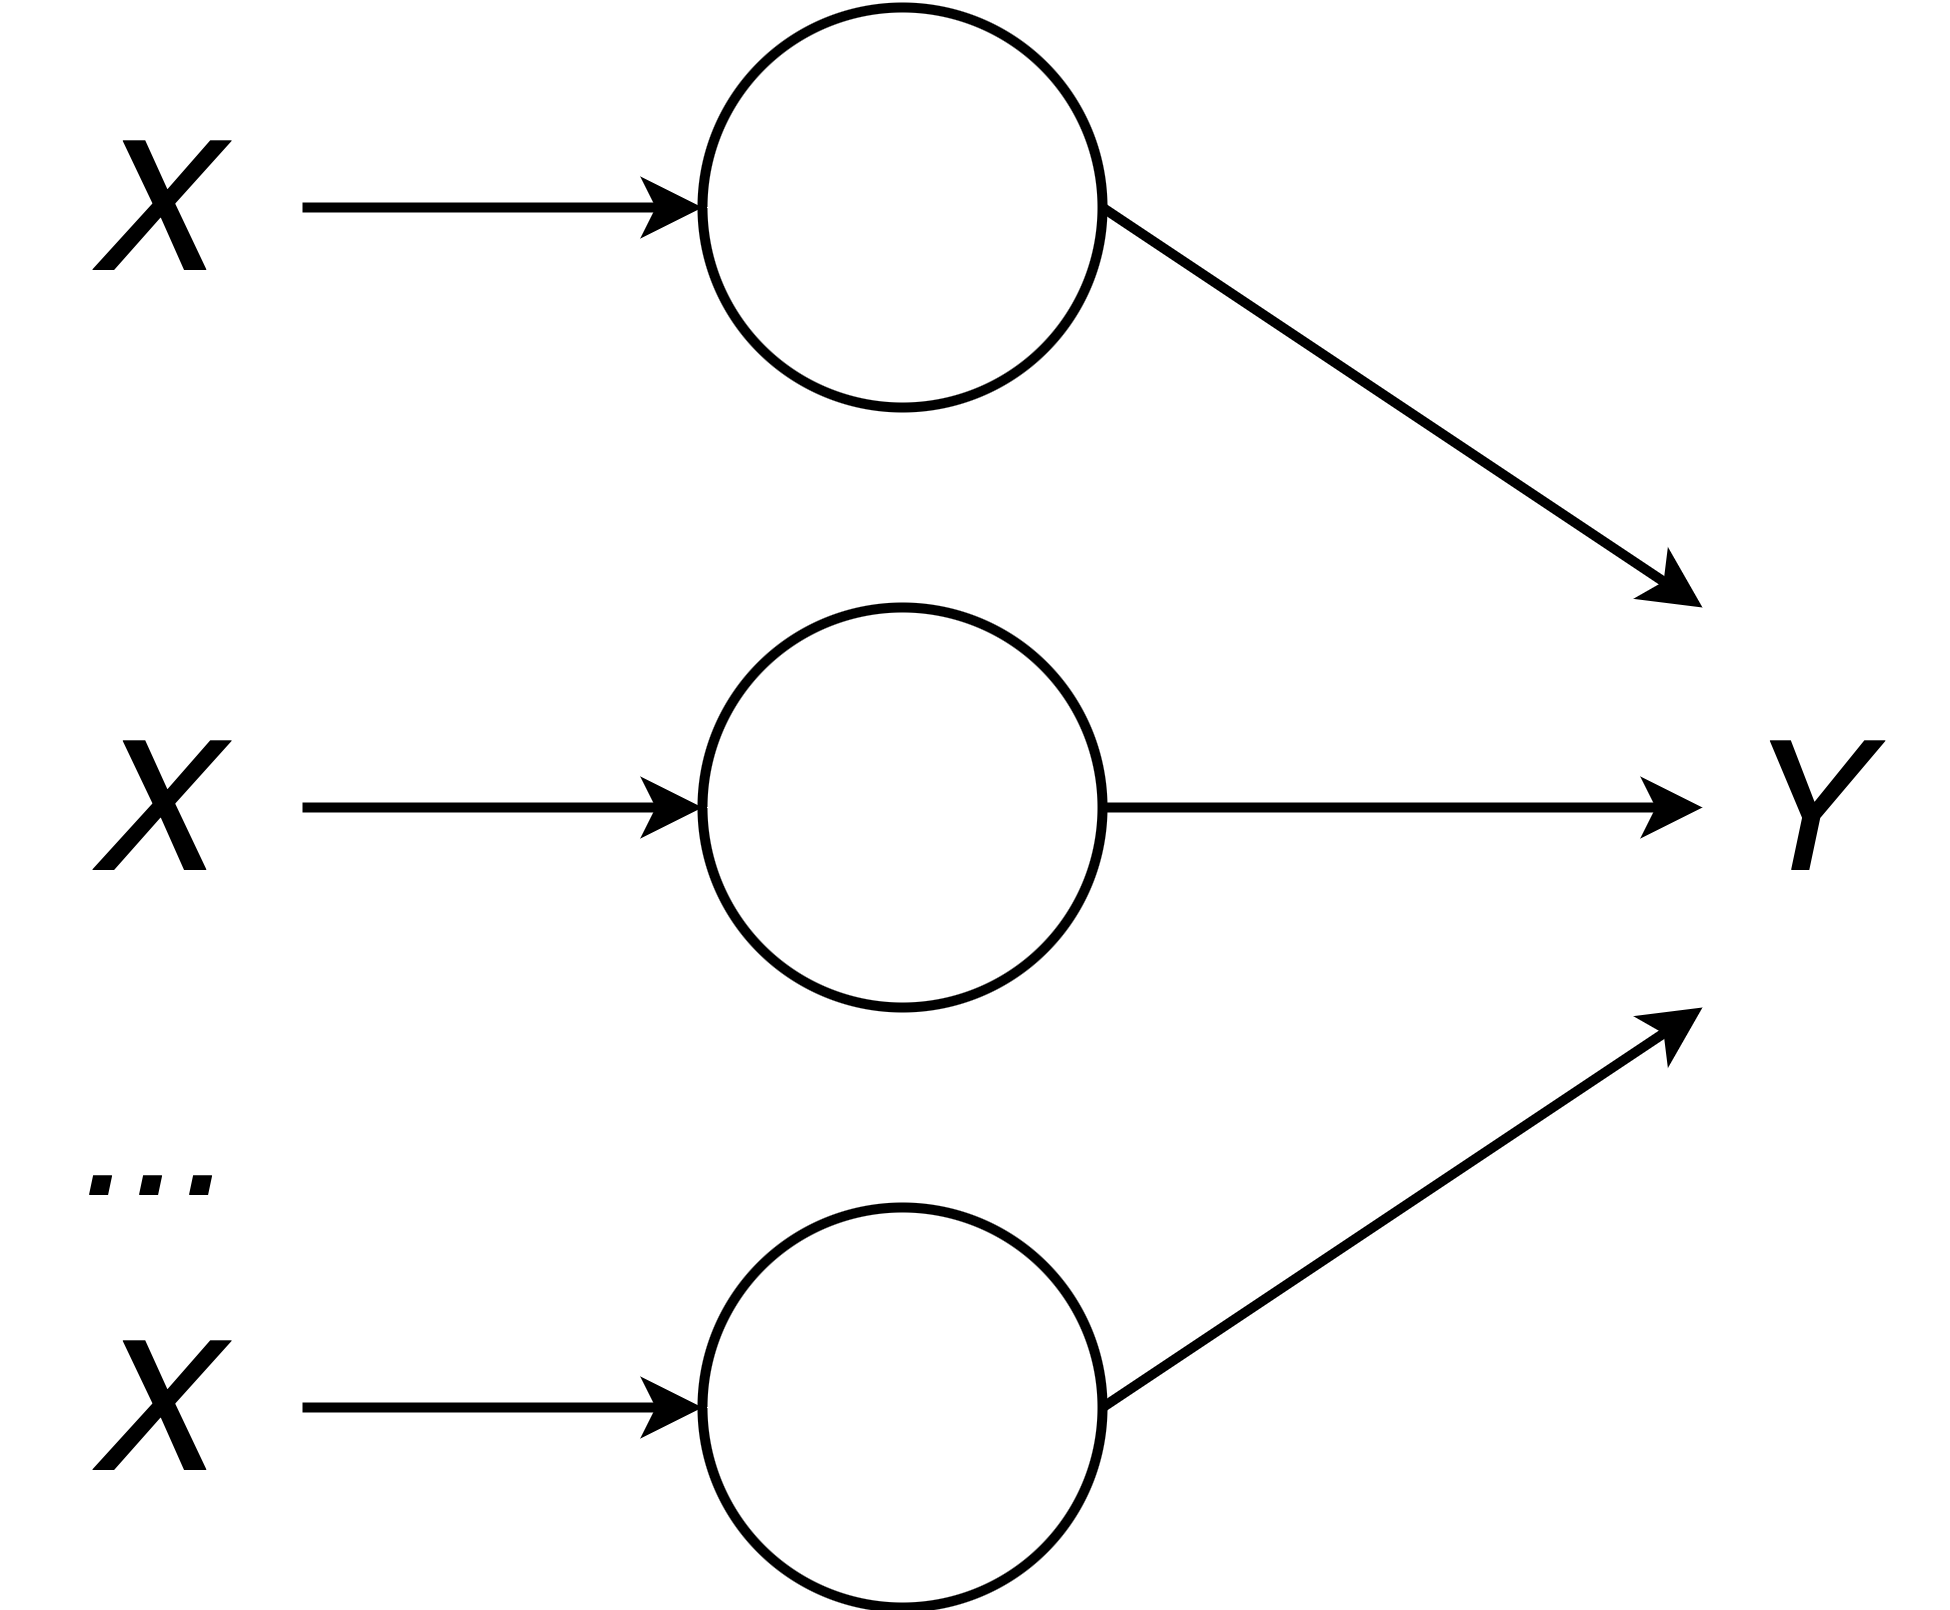
\includegraphics[width=0.6\textwidth]{man-source/images/ch1/pic0-2.png}
  \caption{Слой нейронных элементов}
  \label{fig:pic0_2}
\end{figure}

Наконец, слои нейронных элементов объединяются в последовательности, формируя общую архитектуру нейронной сети (последовательность слоев, их тип, количество нейронов в каждом слое, функцию активации и т.д.). Итоговая модель способна выполнять аппроксимацию любой непрерывной функции с любой точностью после выполнения обучения \cite{Cybenko1989ApproximationBS}. В процессе обучения данные из некоторой выборки подаются на вход сети с целью определения градиентов изменения параметров нейронных элементов. Одна итерация, в ходе которой модели предъявляются все обучающие примеры, называется эпохой. Данная процедура выполняется до тех пор, пока не будет достигнут ответ сети, полученный с желаемой точностью или пока весовые коэффициенты не войдут в некоторое стационарное состояние. 

Искусственные нейронные сети могут быть классифицированы по различным признакам (например, по характеру обучения, по направлению связей, по архитектуре и т.д.). В литературе часто используется классификация по архитектурному признаку. Согласно ей, выделяют \cite{golovko2017}:

\begin{easylistNum}
    & сети персептронного типа (многослойные персептроны \cite{ivakhnenko1967cybernetics}, рекуррентные (\cite{Elman1990FindingSI}, \cite{Jordan1997SerialOA}), рециркуляционные \cite{Hinton1987LearningRB}, сверточные (\cite{fukushima1980}, \cite{LeCun1989HandwrittenDR}), глубокие);
    & самоорганизующиеся НС (НС Кохонена \cite{kohonen2001}, сети адаптивного резонанса \cite{Grossberg1987CompetitiveLF});
    & релаксационные НС (сети Хопфилда \cite{Hopfield1984}, Хэмминга \cite{Lippmann1987} и двунаправленная ассоциативная память \cite{Kosko1988BidirectionalAM});
    & гибридные НС (сети встречного распространения \cite{HechtNielsen1987}, RBF-сети \cite{Broomhead1988}, нечеткие сети \cite{Jang1997});
    & нейронные иммунные сети \cite{Golovko2010}.
\end{easylistNum}

В данной работе исследуются глубокие нейронные сети, являющиеся развитием архитектур полносвязных сетей (персептронов) и сверточных нейронных сетей.

В настоящий момент сверточные нейронные сети и глубокие архитектуры на их основе являются доминирующими в области компьютерного зрения \cite{LeCun2015}. В основном это связано с тем, что в подобных задачах используются данные с высокой корреляцией между соседними элементами (для цифровых фотографий и видео в качестве этих значений выступают массивы пикселей), а сверточные слои особенно эффективны при обработке именно таких данных \cite{Emmert2020}.

Сверточные нейронные сети базируются на моделях неокогнитрона, предложенной К. Фукусимой \cite{fukushima1980}, и сетях с разделяемыми весами. Первая классическая модель сверточной нейронной сети была разработана ЛеКуном и получила название LeNet-5 \cite{lekun1998}. Сверточные нейросети интегрировали три концепции, называемые локальным рецептивным полем, разделяемыми весовыми коэффициентами и пространственной подвыборкой. Используя локальное рецептивное поле, нейронные элементы первого сверточного слоя могут извлекать простейшие признаки, такие как края, углы и т.д. Сверточная нейронная сеть представляет собой комбинацию сверточных (convolutional) и подвыборочных (pooling) слоев (рисунок \ref{fig:cnn_common_view}), благодаря чему осуществляет нелинейное иерархическое преобразование входной информации. Последний блок сверточной сети представляет собой многослойный персептрон, SVM или любой другой классификатор (на рисунке обозначен как classifier).

\begin{figure}[ht]
	\centering
	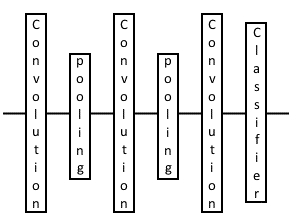
\includegraphics[width=14cm]{man-source/images/ch4/pic4-15.png}
	\caption{Общий вид сверточной нейронной сети}
	\label{fig:cnn_common_view}
\end{figure}
Таким образом, сверточные модели могут включать как сверточные слои, так и некоторое количество полносвязных слоев (завершающие полносвязные слои часто используются как классификаторы признаков, извлеченных на начальных сверточных слоях). %Таким образом, исследование и обучение полносвязных архитектур остается актуальной задачей. 

Несмотря на лидирующее положение сверточных сетей, полносвязные архитектуры также успешно применяются для некоторых задач компьютерного зрения (например, при решении задачи трехмерной реконструкции \cite{mildenhall2020nerf}). Далее в работе будет показано, что сверточный слой может быть представлен с помощью разряженного слоя. Таким образом, исследование и обучение полносвязных архитектур остается актуальной задачей. 

Cтрогого определения понятия глубокой нейронной сети не существует, но ее можно определить как искусственную нейронную сеть с архитектурой персептронного типа, имеющую более двух скрытых слоев нейронных элементов.

В общем случае глубокая нейронная сеть (deep neural network -- DNN) представляет собой нейросетевую модель с множеством слоев нейронных элементов. Рассмотрим полносвязную нейросетевую модель -- многослойный персептрон (рисунок~\ref{fig:pic1_1}). Известно, что такая сеть осуществляет глубокое иерархическое преобразование входного пространства образов \cite{n5}. 

\begin{figure}[H]
  \centering
  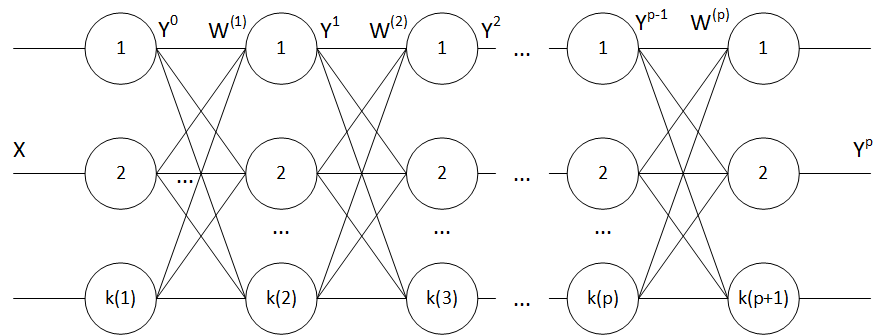
\includegraphics[width=\textwidth]{man-source/images/ch1/pic1-1.png}
  \caption{Глубокая нейронная сеть}
  \label{fig:pic1_1}
\end{figure}

Первый скрытый слой выделяет низкоуровневое пространство признаков входных данных, второй слой определяет пространство признаков более высокого уровня абстракции и т.д. \cite{n3}. 

Выходное значение $j$-го нейрона $k$-го слоя определяется следующим образом:

\begin{equation}
y_j^k=F(S_j^k),
\end{equation}

\begin{equation}
S_j^k=\sum_{i=1} w_{ij}^ky_i^{k-1}+T_j^k,
\end{equation}
где $F(\cdot)$ -- функция активации нейронного элемента \textit{k}-го слоя,\\
$S_j^k$ -- взвешенная сумма $j$-го нейрона $k$-слоя,\\
$w_{ij}^k$ -- весовой коэффициент между $i$-ым нейроном ($k$-1)-го слоя и $j$-м нейроном $k$-го слоя,\\
$T_j^k$ -- пороговое значение $j$-го нейрона $k$-го слоя.

Для первого слоя НС, называемого распределительным, справедливо		
\begin{equation}
y_j^0=x_j.
\end{equation}

В матричном виде выходной вектор $k$-го слоя 

\begin{equation}
Y^k=F(S^k)=F((Y^{k-1})^TW^k+T^k),
\end{equation}
где $W^k$ -- матрица весовых коэффициентов $k$-го слоя,\\
$Y^{k-1}$ -- выходной вектор-столбец ($k$-1)-го слоя,\\
$T^k$ -- вектор пороговых значений нейронов $k$-го слоя.

Если глубокая нейронная сеть используется для классификации образов, то выходные значения сети часто определяются на основе функции активации \textbf{softmax} \cite{golovko2017}: 		

\begin{equation}
y_j^F=softmax(S_j)=\frac{e^{S_j}}{\sum_i e^{S_i}}.
\end{equation}
В этом случае значения, получаемые на последнем слое нейронной сети, отражают вероятность принадлежности данного образа к определенному классу.
%Большинство современных архитектур нейросетевых моделей, решающих задачи компьютерного зрения (классификация, идентификация и детекция объектов, аннотирование и генерация изображений и др.) содержат в своем составе сверточные слои. При этом такие модели могут включать как чисто сверточные слои, так и некоторое количество полносвязных слоев. Однако, и те, и другие называются в этом случае сверточными нейронными сетями. Далее будет показано, что сверточный слой может быть представлен с помощью полносвязного. 

%Интенсивность исследований в области нейронных сетей никогда не выражалась однородным течением. Так, зародившись в работах ... в начале 1940 годов, исскуственным нейронным сетям были посвящены концептуальные и важные работы того времени, которые, однако, были забыты после опубликования работы ... в 1969 году. В данной работе был проведен анализ персептронной модели и выявлены его основные ограничения. Данная работа повлияла на развитие теории и, вплоть до ..., теория не развивалась. С предложенным Дж. Хинтоном методом обратного распространения количество работ в этой области стало увеличиваться, однако, интерес к самим моделям по-преждему находился на недостаточном уровне. Так не безосновательно считалось, что обучение нейронных сетей (в частности, персептронных моделей) с более чем двумя скрытыми слоями бесперспективно. Это было главным образом связано с количеством В 2006 году Дж. Хинтоном была предложен иной подход к обучению так называемых глубоких моделей, который ознаменовал начало новой эпохи в развитии теоретических работ в данной области. Развитие вычислительной техники, с другой стороны, ознаменовало новый виток в реализации возможностей обучения и использования подобных моделей.

% Успехи, достигнутые сегодня в этой области, удивляют и дают основания для продолжения исследования возможностей данных моделей и методов их обучения. 

\section{Проблемы обучения глубоких моделей}

Теория нейронных сетей не развивалась равномерно. Нередко причинами приостановок в исследованиях являлось отсутствие доступных на определенный момент времени эффективных методов обучения моделей. 

Начиная с первых моделей ИНС, описанных в работе У. Мак-Каллока и У. Питтса \cite{mcculloch43a} в 1943 году, искусственным нейронным сетям были посвящены концептуальные и важные работы того времени (например, \cite{hebb1949}, \cite{widrow1960}). В 1959 году Ф. Розенблатт предложил модель персептрона \cite{rosenblatt1959}. Однако, после опубликования монографии М. Минского и С. Пайперта <<Персептроны>> в 1969 году \cite{minsky69perceptrons} крупные исследования в этой области были приостановлены. В этой работе был проведен анализ персептронной модели и выявлены ее основные ограничения, в том числе касающиеся невозможности эффективного решения существующими на тот момент моделями некоторых задач (например, задач инвариантного представления образов). %Это повлияло на развитие нейронных сетей и, вплоть до 1985 года, теория не развивалась. 

В конце 1970-х годов произошел очередной всплеск работ, посвященных нейросетевым моделям (например, \cite{Grossberg1976}, \cite{Kohonen1977}).
В 1986 году Д. Румельхартом, Дж. Хинтоном и Р. Вильямсом в работе \cite{rumelhart1986learning} был предложен метод обратного распространения ошибки для обучения многослойных моделей. Результаты, изложенные в данной работе, открыли теоретические возможности для обучения моделей с большим количеством слоев.  Однако, вплоть до середины 2000-х годов сети с количеством слоев три и более широко не применялись, так как считалось, что использование глубоких моделей не дает существенного прироста в эффективности по сравнению с другими подходами. Неэффективность была связана с проблемой <<исчезающего>> градиента. Она проявляется в том, что при обучении глубокой нейронной сети методом обратного распространения ошибки значения градиентов весовых коэффициентов первых слоев сети быстро становятся близкими к нулю, в результате весовые коэффициенты таких слоев практически не изменяются \cite{n5}. Это существенно замедляет процесс обучения, делая невозможным практическое применение подобных моделей по сравнению с другими существовавшими на тот момент времени методами (например, \cite{Corinna1995}).

Тем не менее, проводя аналогии с многоуровневыми нейронными архитектурами в человеческом мозге (в частности, строением вентральной зрительной системы), было понятно, что подобный тип искусственных нейронных сетей обладает полезными свойствами, позволяя формировать многоуровневую иерархию признаков \cite{Behnke2003}.

В 2006 году Джеффри Хинтоном был предложен подход к обучению глубоких моделей, который ознаменовал начало новой эпохи в развитии теоретических работ в данной области \cite{n1}.

В предложенном методе использовался <<жадный>> алгоритм послойного предобучения глубоких нейронных сетей (greedy layer-wise algorithm) \cite{Hinton2009}, основанный на применении ограниченных машин Больцмана, последовательно формируемых и обучаемых из слоев глубокой нейронной сети. 

С этой работы фактически начался новый подъем в исследованиях нейронных сетей, который длится до настоящего времени. За последующие годы в области компьютерного зрения благодаря применению глубоких нейронных сетей удалось значительно улучшить результаты для различных задач, включая классификацию, детекцию, сегментацию объектов на изображении, генерацию текстовых описаний к изображениям, генерацию изображений по текстовым описаниям и т.д.  % Последовавший всплеск количества работ, посвященных обучению и применению глубоких сетей в различных сферах, позволил в течение последующих нескольких лет значительно улучшить первоначальные результаты.

В течение следующих лет сместился основной акцент в исследованиях -- вместо послойного обучения стали применяться методы, позволяющие обучать глубокие нейронные сети, начиная с произвольной начальной инициализации, без использования предобучения (например, стохастический градиентный спуск с использованием функции активации ReLU и ее вариантов). Однако, применение таких подходов не снижает требований к объему обучающей выборки, которая в идеальных теоретических условиях должна быть сравнима с числом настраиваемых параметров модели, поскольку большие модели, обучаемые на малых выборках, с большей вероятностью будут переобучаться. Результатом этого является отличная приспособленность модели к обучающей выборке, но плохая обобщающая способность, т.е. неэффективность сети на тестовых данных. Таким образом, объем используемой обучающей выборки для глубоких нейронных сетей остается по-прежнему критичным фактором для обучения. Даже наличие подходящей по объему выборки не гарантирует успешное завершение обучения, так как подготовка больших моделей может повлечь неприемлемые аппаратные издержки (\cite{alpaca2023}, \cite{alpacagithub}, \cite{zhang2022opt}).

\section{Методы обучения}

Рассмотрим основные методы, применяемые для обучения глубоких нейронных сетей.

Существуют два основных подхода к обучению глубоких нейронных сетей, оба из которых используют предобучение:

\begin{easylistNum}    
    & обучение с использованием предобучения на большой обучающей выборке и любого оптимизирующего метода для настройки параметров нейронной сети (I тип);
	& обучение с использованием неконтролируемого предобучения (II~тип).
\end{easylistNum}

Предобучение I типа представляет собой обучение модели с использованием метода обратного распространения ошибки \cite{Glorot2011}, некоторого оптимизирующего метода и активационных функций ReLU и ее вариантов в качестве функций активации нейронов \cite{LeCun2015}, а затем дообучение полученной модели для новой выборки (transfer learning). 

Среди основных оптимизирующих методов, применяемых для предобучения I типа, выделяют \cite{Goodfellow2017}:

\begin{easylistNum}
	& SGD (стохастический градиентный спуск). В данном методе корректировка настраиваемых параметров ИНС выполняется в направлении, противоположном вектору градиента функции потерь \cite{Haykin2006};
	& метод Нестерова. Обучение методом стохастического градиентного спуска нередко происходит очень медленно. Импульсный метод позволяет ускорить обучение, особенно в условиях высокой кривизны, небольших, но устойчивых градиентов или зашумленных градиентов. В импульсном методе вычисляется экспоненциально затухающее скользящее среднее прошлых градиентов и продолжается движение в этом направлении. Метод Нестерова является вариантом импульсного алгоритма, в котором градиент вычисляется после применения текущей скорости \cite{Goodfellow2017};
	& AdaGrad: данный метод по отдельности адаптирует скорости обучения всех настраиваемых параметров ИНС, умножая их на коэффициент, обратно пропорциональный квадратному корню из суммы всех прошлых значений квадрата градиента \cite{Duchi2011};
	& RMSProp. Данный метод является модификацией AdaGrad, которая позволяет улучшить его поведение в невыпуклом случае путем изменения способа агрегирования градиента на экспоненциально взвешенное скользящее среднее. Использование экспоненциально взвешенного скользящего среднего гарантирует повышение скорости сходимости после обнаружения выпуклой впадины, как если бы внутри этой впадины алгоритм AdaGrad был инициализирован заново \cite{Goodfellow2017};
	& Adam. Данный метод можно рассматривать как комбинацию RMSProp и AdaGrad \cite{Kingma2014}. 
	Помимо усредненного первого момента, данный метод использует усредненное значение вторых моментов градиентов.
\end{easylistNum}

I тип фактически представляет собой обучение с нуля, которое осуществляется на больших выборках данных с использованием подходящих аппаратных средств. Предобученные таким образом модели могут быть использованы для решения других задач. Таким образом, современный инженер получает в свое распоряжение репозиторий готовых предобученных моделей, которые могут быть дообучены на небольших выборках данных, предназначенных для решения конкретной задачи.

Рассмотрим подробно реализацию предобучения II типа.

Исследование методов предобучения II типа остается актуальной и перспективной задачей, поскольку позволяет существенно сократить объем применяемой обучающей выборки (для малых обучающих выборок позволяет преодолеть переобучение \cite{LeCun2015}) и жесткие требования к используемой аппаратной части.

В общем случае процесс обучения глубоких нейронных сетей с послойным предобучением (предобучением II типа) можно описать последовательностью из двух этапов \cite{n1, n2, n3, n4}: 
\begin{easylistNum}
	& предобучение нейронной сети методом послойного обучения, начиная с первого слоя  (pre-training). Такое обучение осуществляется неконтролируемо;
	& настройка синаптических связей всей сети (fine-tuning) при помощи алгоритма обратного распространения ошибки или алгоритма <<бодрствования и сна>> (wake-sleep algorithm) \cite{hinton1995}.
\end{easylistNum}

%Предобучение I типа осуществляется в два этапа . На первом этапе производится предварительная послойная настройка весов нейронной сети. Процедура начинается с первого слоя и выполняется без учителя (неконтролируемо). На втором этапе выполняется <<тонкая>> настройка весов нейронной сети, используя, например, алгоритм обратного распространения.

\textbf{Первый этап} является <<ядром>> всего подхода.
Выделяют два основных подхода к реализации первого этапа (рисунок~\ref{fig:pic1_2}). %Первый -- метод Хинтона, основанный на применении ограниченных машин Больцмана. Второй подход базируется на обучении автоэнкодерных нейронных сетей. 
В обоих этих методах формирование вспомогательных архитектур (RBM, автоэнкодеров) осуществляется из структуры исходной сети. 

\begin{figure}[H]
  \centering
  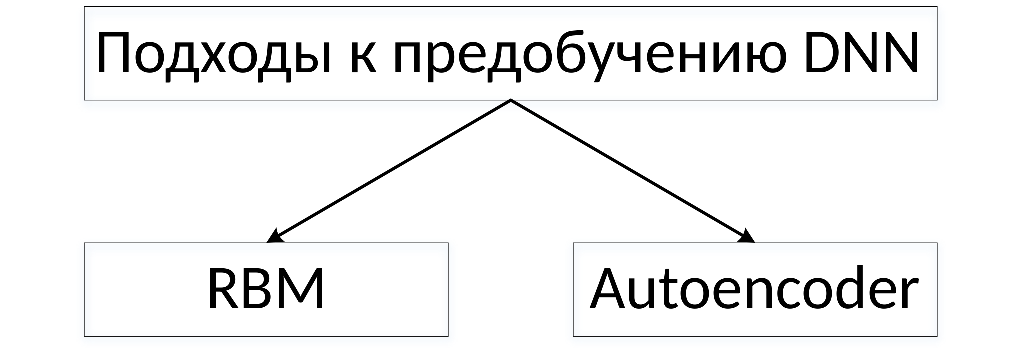
\includegraphics[width=0.7\textwidth]{man-source/images/ch1/pic1-2.pdf}
  \caption{Методы предварительного обучения глубоких нейронных сетей}
  \label{fig:pic1_2}
\end{figure}

Первый подход основывается на представлении каждого слоя нейронной сети в виде ограниченной машины Больцмана (RBM). При использовании второго, автоэнкодерного, подхода, каждый слой  представляется автоассоциативной нейронной сетью.

Рассмотрим каждый из этих подходов подробнее.

% \subsection{Алгоритм обучения ГНС с использованием RBM} \label{subsect1_3_2}
\def\slantfrac#1#2{ \hspace{3pt}\!^{#1}\!\!\hspace{1pt}/
  \hspace{2pt}\!\!_{#2}\!\hspace{3pt}
}

При предобучении ГНС в соответствии с \textbf{первым подходом} осуществляется последовательное конструирование RBM-сетей из параметров скрытых слоев ГНС и их обучение. 

Для понимания подхода рассмотрим модель RBM.

Ограниченная машина Больцмана состоит из двух слоев стохастических бинарных нейронных элементов, которые соединены между собой двунаправленными симметричными связями (рисунок~\ref{fig:pic1_3}). Входной слой нейронных элементов называется видимым (слой $X$), а выходной -- скрытым (слой $Y$). Ограниченная машина Больцмана может генерировать любое дискретное распределение, если используется достаточное количество нейронов скрытого слоя \cite{n5}.

\begin{figure}[H]
  \centering
  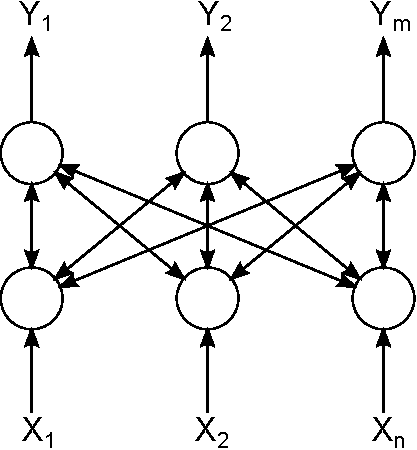
\includegraphics[width=0.4\textwidth]{man-source/images/ch1/pic1-3.pdf}
  \caption{Ограниченная машина Больцмана}
  \label{fig:pic1_3}
\end{figure}	

В данной модели состояния видимых и скрытых нейронов меняются в соответствии с вероятностной версией сигмоидной функции активации:
	
\begin{equation}
	p(y_j\lvert x)=\frac{1}{1+e^{-S_j}},\ S_j=\sum_i^n w_{ij}x_i+T_j,
\end{equation}
	
\begin{equation}
	p(x_i\lvert y)=\frac{1}{1+e^{-S_i}},\ S_i=\sum_j^m w_{ij}y_j+T_i,
\end{equation}
где $S_i, S_j$ -- взвешенные суммы видимого и скрытого слоев,\\
$T_i, T_j$ -- пороговые элементы видимого и скрытого слоев соответственно.
	
Состояния видимых и скрытых нейронных элементов принимаются независимыми:
	
\begin{equation*}
\begin{aligned}
	P(x \lvert y) = \prod_{i=1}^n P(x_i \lvert y),\\
	P(y \lvert x) = \prod_{j=1}^m P(y_j \lvert x).
\end{aligned}	
\end{equation*}
	
Таким образом, состояния всех нейронных элементов ограниченной машины Больцмана определяются через распределение вероятностей. В RBM нейроны скрытого слоя являются детекторами признаков, которые сохраняют закономерности входных данных. Основная задача обучения состоит в воспроизведении распределения входных данных на основе состояний нейронов скрытого слоя как можно точнее. Для достижения этого применяется процедура CD-\textit{k}. В главе 2 будет подробна описана данная процедура и приведен вывод классических правил обучения RBM. %Это эквивалентно  максимизации функции правдоподобия путем модификации синаптических связей нейронной сети. Покажем основные этапы вывода правил обучения для RBM.

При предобучении ГНС на базе RBM вначале создается RBM-модель из первого скрытого слоя ГНС. Для данной RBM входные данные поступают на видимый слой нейронных элементов и используя CD-$k$ процедуру вычисляются состояния скрытых $P(y \lvert x)$ и видимых нейронов $P(x \lvert y)$. В процессе выполнения данной процедуры в течение заданного количества эпох изменяются весовые коэффициенты и пороговые значения сети RBM, которые затем фиксируются. Следующим берется второй скрытый слой глубокой нейронной сети и конструируется новая RBM. Входными данными для нее являются данные с предыдущего слоя (выходные данные, полученные первой RBM). Выполняется обучение новой модели и процесс продолжается для всех последующих слоев нейронной сети, за исключением, возможно, самого последнего (включение последнего слоя в процесс предобучения зависит от решаемой задачи -- например, для задачи классификации предобучение последнего слоя не требуется, так как он должен обучаться с учителем), как показано на рисунке~\ref{fig:pic1_4}. 

\begin{figure}[H]
  \centering
  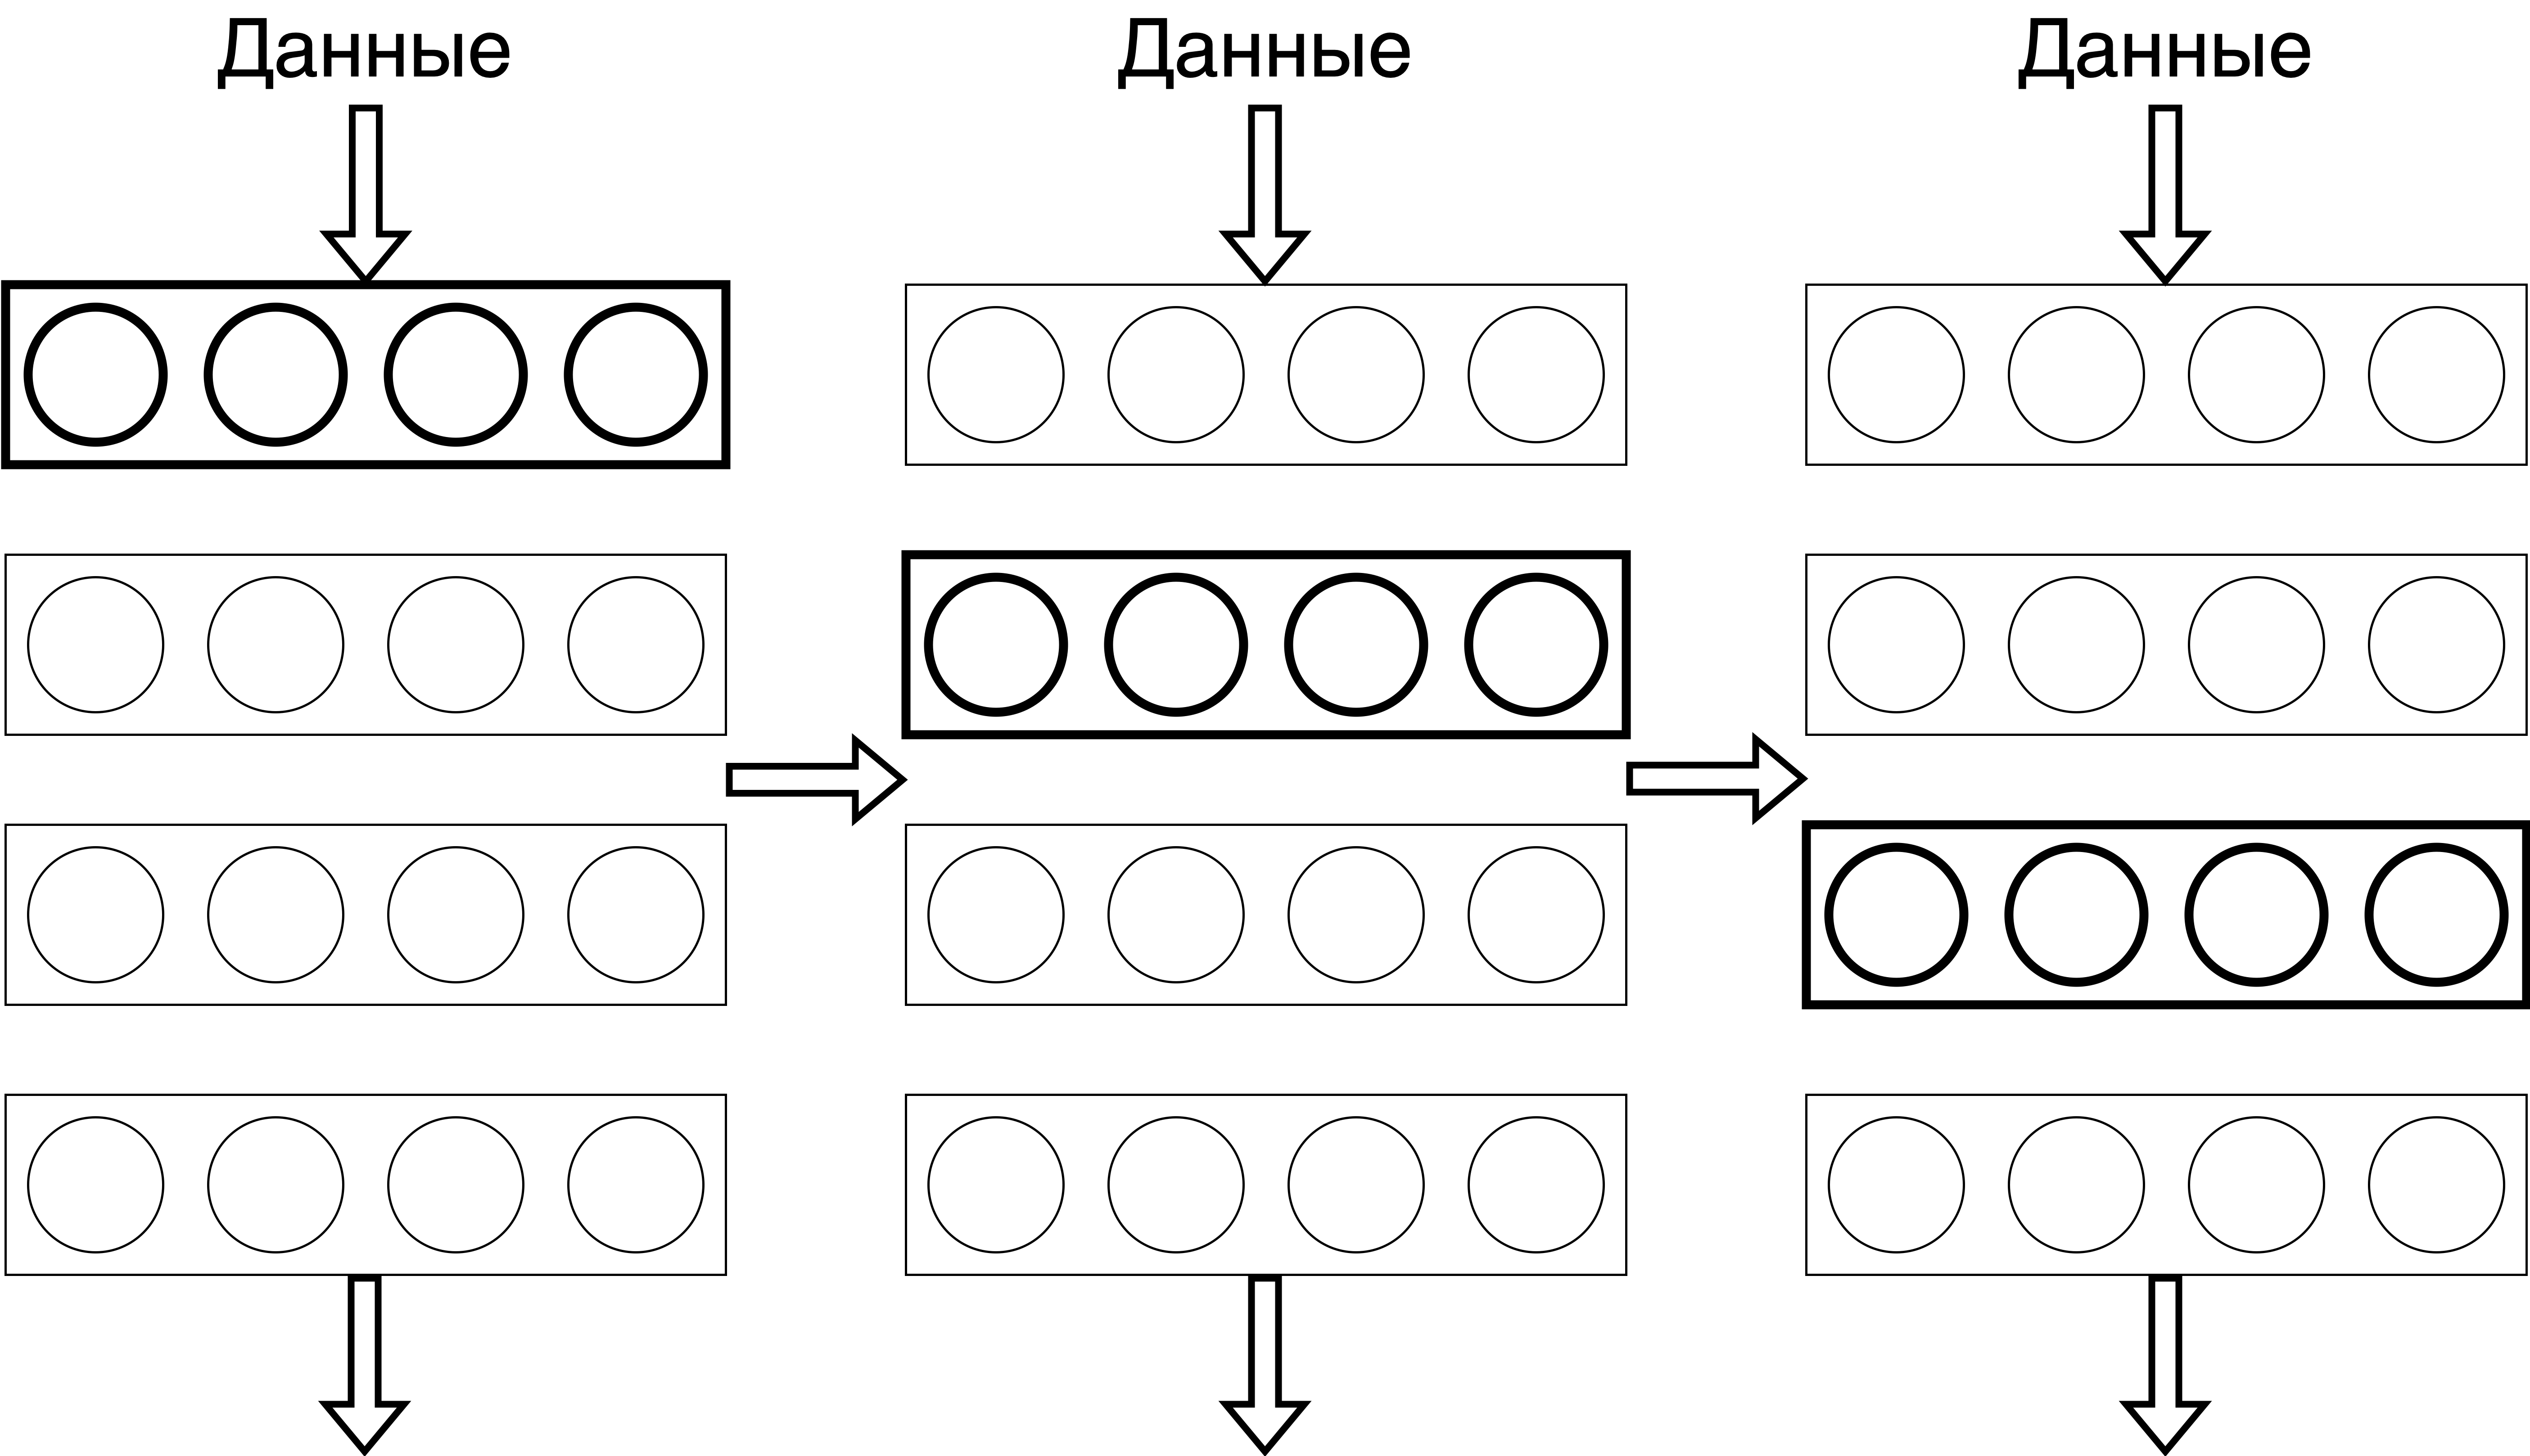
\includegraphics[width=\textwidth]{man-source/images/ch1/pic1-4.png}
  \caption{<<Жадный>> алгоритм послойного обучения}
  \label{fig:pic1_4}
\end{figure}

% \section{Автоэнкодерный метод предобучения} \label{subsect1_3_3}

При предобучении ГНС в соответствии со \textbf{вторым подходом} \cite{n6}, вначале обучается первый слой ГНС как автоассоциативная нейронная сеть с целью минимизации суммарной ошибки реконструкции данных, затем обучается второй слой ГНС и так далее. Для обучения каждого слоя можно использовать алгоритм обратного распространения ошибки. 

%После этого осуществляется точная настройка синаптических связей всей сети (fine tuning), используя алгоритм обратного распространения ошибки. 
	
Рассмотрим персептрон с тремя скрытыми слоями (рисунок \ref{fig:pic1_5}). Тогда в соответствии с автоэнкодерным методом, прежде всего, берутся первые два слоя нейронной сети (1 и 2) и на базе их конструируется автоассоциативная (рециркуляционная) нейронная сеть (1-2-1), то есть добавляется восстанавливающий слой (рисунок \ref{fig:pic1_6}). 
	
\begin{figure}[H]
  \centering
  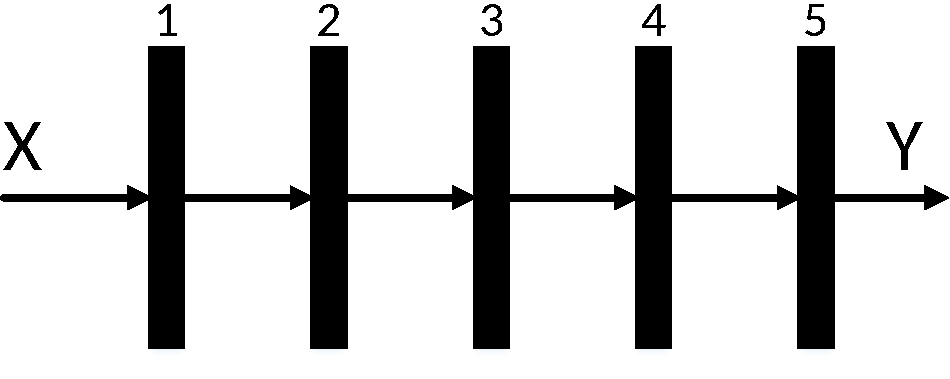
\includegraphics[width=0.7\textwidth]{man-source/images/ch1/pic1-5.pdf}
  \caption{Персептрон с тремя скрытыми слоями}
  \label{fig:pic1_5}
\end{figure}	

\begin{figure}[H]
  \centering
  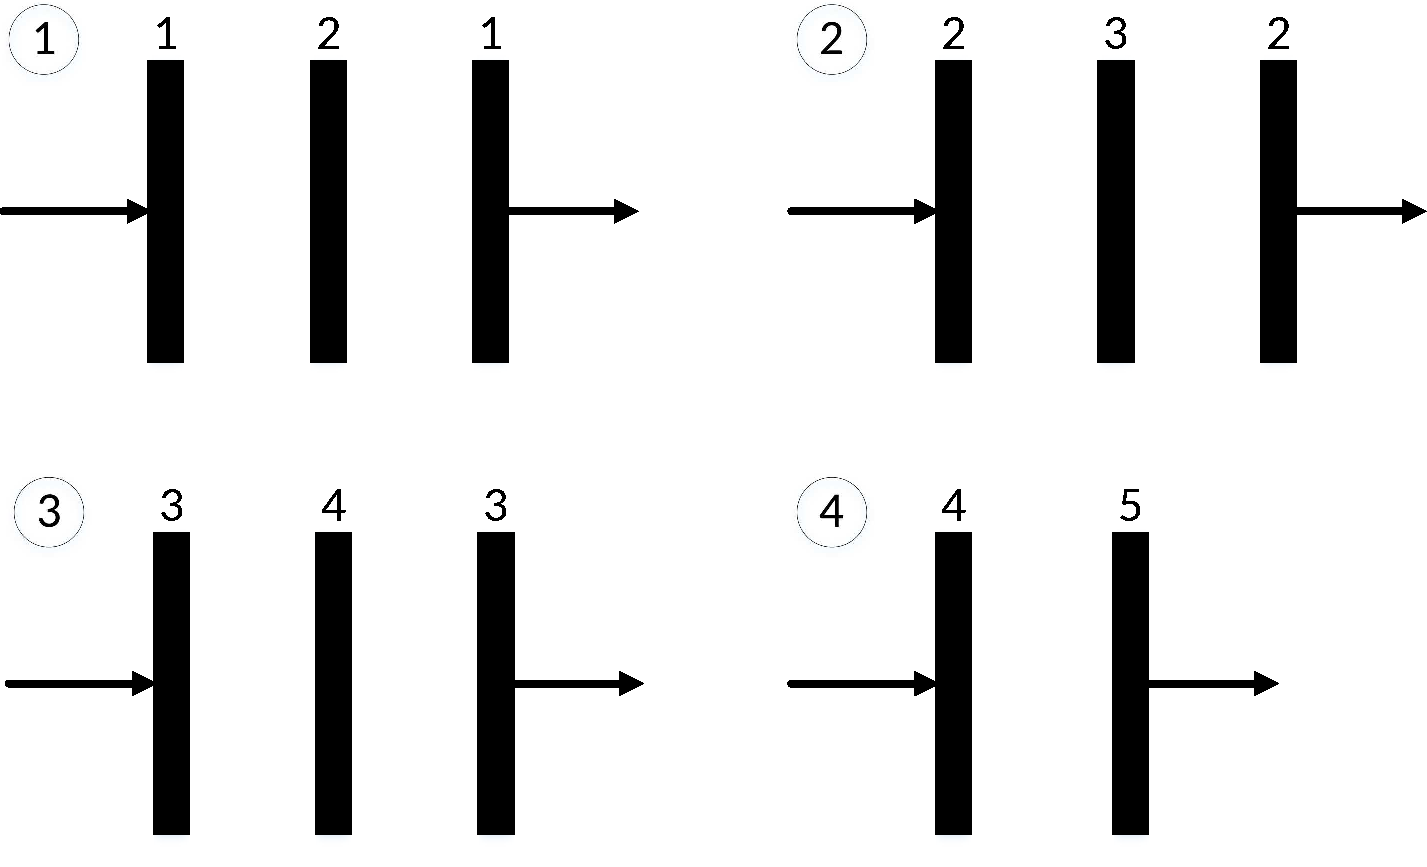
\includegraphics[width=0.7\textwidth]{man-source/images/ch1/pic1-6.pdf}
  \caption{Автоэнкодерный метод обучения}
  \label{fig:pic1_6}
\end{figure}

Затем, происходит обучение такой сети, например, при помощи алгоритма обратного распространения ошибки с целью минимизации ошибки реконструкции данных. 
	
После этого отбрасывается восстанавливающий слой (последний слой) автоассоциативной сети, фиксируются веса скрытого слоя, и конструируется автоассоциативная сеть из следующих двух слоев нейронной сети (2-3-2), которая обучается на основе данных, поступающих с предыдущего (2-го слоя). Процесс продолжается до последнего или предпоследнего слоя, как это схематично изображено на рисунке \ref{fig:pic1_6}. %В результате послойного обучения получается предварительно обученная нейронная сеть. Далее осуществляется точная настройка (fine-tuning) посредством, например, алгоритма обратного распространения ошибки с учителем.
	
Данный процесс можно представить в виде следующего алгоритма:
\begin{easylistNum}
	& конструируется автоассоциативная сеть с входным слоем $X$, скрытым $Y$ и выходным слоем $X$;
	& обучается автоассоциативная сеть, например при помощи алгоритма обратного распространения ошибки и фиксируются синаптические связи первого слоя $W_1$;
	& берется следующий слой глубокой нейронной сети и снова формируется автоассоциативная сеть аналогичным образом;
	& используя настроенные синаптические связи предыдущего слоя $W_1$, подаются входные данные на вторую автоассоциативную сеть и она обучается аналогичным образом. В результате получаются весовые коэффициенты второго слоя $W_2$;
	& процесс продолжается до последнего или предпоследнего слоя нейронной сети.
	%& Берется последний слой нейронной сети и обучается с учителем.
	%& Обучается вся сеть для точной настройки параметров при помощи алгоритма обратного распространения ошибки.
\end{easylistNum}

Для обоих подходов (RBM и автоэнкодерный), с помощью реализации такого неконтролируемого предобучения можно получить приемлемую начальную инициализацию настраиваемых параметров глубокой нейронной сети. 

%\textbf{На втором этапе} производится точная настройка параметров всей сети при помощи алгоритма обратного распространения ошибки или алгоритма <<бодрствования и сна>> (wake-sleep algorithm).
	
% \section{Этап <<тонкой>> настройки глубокой НС}

На \textbf{втором этапе}, иначе называемом этапом <<тонкой настройки>> нейронной сети или fine-tuning, выполняется дообучение всей ГНС некоторым традиционным подходом (например, алгоритмом обратного распространения ошибки или <<бодрствования и сна>>).

Критически важным для этого этапа является начальная инициализация весов и порогов. Если такая инициализация выполнена в ходе предобучения, то сеть начинает процесс <<тонкой настройки>> с <<хороших>> начальных значений, что обуславливает быструю сходимость.

Если же предобучение отсутствует и используется традиционная <<поверхностная>> схема обучения со случайной инициализацией параметров, обучение сети может быстро остановиться и, как результат, приемлемая обобщающая способность не будет достигнута.

В дальнейшем под предобучением будем понимать предобучение II~типа, проводимое с использованием RBM-сетей, если не указано иного. 

\section{Критерии минимизации при обучении}

При обучении ГНС (например, на этапе <<тонкой настройки>>, если сеть предобучалась) важно определить критерий минимизации. Наиболее известными и используемыми в настоящий момент функциями ошибок являются функция квадратичной ошибки (SE)

\begin{equation}
	\label{MSE}
	E_{SE} = \frac{1}{2}\sum_{j=1}^{n}(y_j - t_j)^2
\end{equation}
и кросс-энтропийная функция (CE) -- случай мультиклассовой классификации

\begin{equation}
	\label{CE_multiclass}
	E_{CE_{mult}} = -\sum_{j=1}^{n}t_j\log(y_j),
\end{equation}
где $n$ -- количество нейронных элементов в последнем слое,\\
$y_j$ -- выход нейрона $j$,\\
$t_j$ -- эталонное значение этого нейрона,\\
множитель $\frac{1}{2}$ введен для удобства вычислений.

Формула \ref{MSE} справедлива для одного обучающего примера. Для $L$ обучающих примеров она запишется в следующем виде (MSE -- среднеквадратичная ошибка):

\begin{equation}
	\label{MSE_L}
	E_{MSE} = \frac{1}{2L}\sum_{k=1}^{L}\sum_{j=1}^{n}(y_j^k - t_j^k)^2.
\end{equation}

При обучении автоэнкодеров часто применяется кросс-энтропийная функция, обобщающая двухклассовый случай (\cite{Amaral2013}):

\begin{equation}
	\label{CE}
	E_{CE} = -\sum_{j=1}^n(t_j\log(y_j) + (1-t_j)\log(1-y_j)).
\end{equation}

Согласно методу обратного распространения ошибки, для настройки весовых коэффициентов и порогов применяются следующие правила, получаемые в соответствии с методом градиентного спуска:

\begin{equation}
	w_{i-1,i} = w_{i-1, i} - \alpha \frac{\partial E}{\partial w_{i-1, i}},
\end{equation}
\begin{equation}
	T_i = T_i - \alpha \frac{\partial E}{\partial T_i},
\end{equation}
где $w_{i-1,i}$ -- весовые коэффициенты для \textit{i}-го обрабатывающего слоя нейронной сети, \textit{i} изменяется от 1 до \textit{N},\\
\textit{N} -- количество обрабатывающих слоев нейронной сети,\\
$\alpha$ -- скорость обучения, а соответствующие градиенты находятся по формулам:

\begin{equation}
	\label{weights_delta}
	\frac{\partial E}{\partial w_{i-1, i}} = \frac{\partial E}{\partial S_i} y_{i-1},
\end{equation}
\begin{equation}
	\label{biases_delta}
	\frac{\partial E}{\partial T_i} = \frac{\partial E}{\partial S_i},
\end{equation}
где $\frac{\partial E}{\partial S_i}$ -- частная производная по взвешенной сумме для i-го слоя НС,\\
$y_{i-1}$ -- выход $i-1$-го слоя НС.


Частные производные по взвешенным суммам $S_i$ получаются в соответствии со следующими выражениями:
\begin{equation}
	\label{last_layer_error}
	\frac{\partial E}{\partial S_i} = (y_i - t_i)F'(S_i),
\end{equation}

\begin{equation}
	\label{sum_rec_common}
	\frac{\partial E}{\partial S_{i-1}} = \Bigg(\sum_{i}\frac{\partial E}{\partial S_i}w_{i-1, i}\Bigg)F'(S_{i-1}),
\end{equation}
где $F$ -- функция активации нейронных элементов.

Формула \ref{last_layer_error} используется для последнего слоя НС, а формула \ref{sum_rec_common} -- для других слоев, кроме последнего.

Формула \ref{last_layer_error} актуальна для случая, если используется целевая функция $E_{MSE}$. Для случая $E_{CE}$ она будет иметь следующий вид:

\begin{equation}
	\label{last_layer_error_ce}
	\frac{\partial E}{\partial S_i} = \frac{y_i - t_i}{y_i(1-y_i)}F'(S_i).
\end{equation}

В случае использования логистической функции, формула \ref{last_layer_error_ce} упрощается, поскольку в этом случае $F'(S_i)=y_i(1-y_i)$:

\begin{equation}
	\frac{\partial E}{\partial S_i} = y_i - t_i.
\end{equation}

Формулы \ref{weights_delta}, \ref{biases_delta} и \ref{sum_rec_common} справедливы как для случая $E_{MSE}$, так и для $E_{CE}$.

Для $E_{CE_{mult}}$ эти формулы справедливы для функции активации \textbf{softmax} на последнем слое нейронной сети. Покажем это.

Имеем

\begin{equation}
	\label{common_E}
	\frac{\partial E_{CE_{mult}}}{\partial S_i} = \sum_{k=1}^{n} \frac{\partial E_{CE_{mult}}}{\partial y_k}\frac{\partial y_k}{\partial S_i} = \frac{\partial E_{CE_{mult}}}{\partial y_i}\frac{\partial y_i}{\partial S_i} + \sum_{k\neq i}\frac{\partial E_{CE_{mult}}}{\partial y_k}\frac{\partial y_k}{\partial S_i}.
\end{equation}

Очевидно, 
\begin{equation}
\label{part_deriv_y}
\frac{\partial E_{CE_{mult}}}{\partial y_i} = -\frac{t_i}{y_i}.
\end{equation}

Учитывая, что
\begin{equation}
	y_i = \frac{e^{S_i}}{\sum_{k=1}^{n} e^{S_k}},
\end{equation}
где $i$ -- индекс последнего слоя сети,\\
$S_i$ -- соответствующая взвешенная сумма, найдем значения частной производной $\frac{\partial y_i}{\partial S_k}$.
\begin{easylistNum}
	& Случай $i = k$:
	\begin{multline}
		\label{part1_deriv_S}
		\frac{\partial y_i}{\partial S_i} = \frac{e^{S_i}\sum e^{S_k} - e^{2S_i}}{(\sum e^{S_k})^2} = \\ = \frac{e^{S_i}\sum e^{S_k}}{(\sum e^{S_k})^2}-\frac{e^{2S_i}}{(\sum e^{S_k})^2}=y_i - y_i^2 = y_i(1-y_i);
	\end{multline}
	& $i \neq k$:
	\begin{equation}
		\label{part2_deriv_S}
		\frac{\partial y_k}{\partial S_i} = -e^{S_k}\Big(\sum e^{S_i}\Big)^{-2}e^{S_i} = -y_ky_i.
	\end{equation}
\end{easylistNum}

Подставляя полученные выражения \ref{part1_deriv_S}, \ref{part2_deriv_S} и \ref{part_deriv_y} в \ref{common_E}, получим
\begin{equation}
	\frac{\partial E_{CE_{mult}}}{\partial S_i} = -t_i(1-y_i) + \sum_{k\neq i}t_ky_i = -t_i + y_i\sum_{k=1}^{n}t_k = y_i - t_i.
\end{equation}

\section{Выводы}

\begin{easylistNum}
    & Дано описание основных понятий теории искусственных нейронных сетей, приведена классификация моделей ИНС.
    & Сформулирована проблема обучения глубоких нейронных сетей, обоснована ее актуальность. Приведены предпосылки развития методов обучения глубоких нейронных сетей.  
    & Рассмотрены существующие методы обучения глубоких нейронных сетей.
    & Описаны основные этапы обучения ГНС с использованием неконтролирумого предобучения, включающие в себя предобучение ГНС и <<тонкую настройку>> модели.
    & Описаны основные подходы к осуществлению неконтролируемого предобучения ГНС, базирующиеся на использовании ограниченных машин Больцмана и автоассоциативных нейронных сетей.
	& Рассмотрены основные критерии минимизации, которые применяются при обучении нейронных сетей, а также дано описание метода обратного распространения ошибки и рассмотрены правила его реализации для различных целевых критериев.
\end{easylistNum}

\chapter{Метод неконтролируемого предобучения}

В данной главе в контексте проблемы обучения ГНС приводится вывод классических правил обучения ограниченной машины Больцмана (restricted Boltzmann Machine), применяемой на этапе неконтролируемого предобучения ГНС.

Предложен альтернативный подход к обучению ограниченной машины Больцмана (\cite{1-A, 4-A, 5-A}), базирующийся на минимизации ошибок восстановления образов на его видимом и скрытом слоях, используя итерации сэмплирования Гиббса. В качестве критериев минимизации используются MSE (mean squared error -- среднеквадратичная ошибка) и CE (cross-entropy loss -- кросс-энтропийная функция потерь). 

Для предлагаемого подхода рассмотрен вывод правил обучения RBM. Показано, что полученные правила обобщают классические правила обучения, полученные в работах Дж. Хинтона.

Для основных случаев предлагаемого подхода приводятся правила обучения CRBM, которые могут быть использованы для предобучения глубоких сверточных нейронных сетей. Также показано, что сверточный слой может быть представлен в виде полносвязного слоя.

Предлагается подход к редуцированию размерности нейросетевых моделей за счет уменьшения количества настраиваемых параметров и количества используемых нейронов после выполнения процедуры предобучения с использованием сетей RBM.

\section{Обучение RBM}

В главе 1 было описано, что одним из методов обучения ГНС является метод предобучения, основывающийся на использовании ограниченных машин Больцмана.

Также, ранее было упомянуто, что основная задача обучения ограниченной машины Больцмана состоит в воспроизведении распределения входных данных на основе состояний нейронов скрытого слоя как можно точнее. Это эквивалентно  максимизации функции правдоподобия путем модификации синаптических связей нейронной сети. Покажем основные этапы вывода классических правил обучения для RBM.

Вероятность нахождения видимого и скрытого нейрона в состоянии $(x, y)$ определяется на основе распределения Гиббса \cite{gibbs1902}:
	
\begin{equation*}
	P(x, y)=\frac{e^{-E(x,y)}}{Z},
\end{equation*}
где $E(x,y)$ -- энергия системы в состоянии $(x,y)$,\\
$Z$ -- параметр, который определяет условие нормализации вероятностей, то есть, условие, при котором сумма вероятностей $P(x, y)$ равняется единице. Данный параметр определяется следующим образом:
	
\begin{equation*}
	Z=\sum_{(x,y)} e^{-E(x,y)}.
\end{equation*}
	
Вероятность нахождения видимых нейронов в определенном состоянии равняется сумме вероятностей  конфигураций $P(x,y)$ по состояниям скрытых нейронов:
	
\begin{equation*}
	P(x)=\sum_y P(x,y)=\sum_y \frac{e^{-E(x,y)}}{Z}=\frac{\sum_y e^{-E(x,y)}}{\sum_{(x,y)} e^{-E(x,y)}}.
\end{equation*}
	
Для нахождения правил модификации параметров модели необходимо максимизировать вероятность воспроизведения состояний видимых нейронов $P(x)$ ограниченной машиной Больцмана. Для того, чтобы определить максимум функции правдоподобия распределения данных $P(x)$ будем использовать метод градиентного подъема в пространстве весовых коэффициентов и пороговых значений сети, где в качестве целевой функции используем функцию логарифмического правдоподобия:
	
\begin{equation*}
	\ln P(x)=\ln \sum_y e^{-E(x,y)}-\ln \sum_{(x,y)} e^{-E(x,y)}.
\end{equation*}
	
Тогда градиент равен
	
\begin{equation*}
	\frac{\partial \ln P(x)}{\partial w_{ij}}=\frac{\partial}{\partial w_{ij}}\ln \sum_y e^{-E(x,y)}-\frac{\partial}{\partial w_{ij}}\ln\sum_{(x,y)} e^{-E(x,y)}.
\end{equation*}
	
Преобразуя последнее выражение, получим
	
\begin{equation*}
	\frac{\partial \ln P(x)}{\partial w_{ij}}=-\frac{1}{\sum_y e^{-E(x,y)}}\sum_y e^{-E(x,y)}\frac{\partial E(x,y)}{\partial w_{ij}}+\frac{1}{\sum_{(x,y)} e^{-E(x,y)}}\sum_{(x,y)} e^{-E(x,y)}\frac{\partial E(x,y)}{\partial w_{ij}}.
\end{equation*}
	
Так как
	
\begin{equation*}
	P(x,y)=P(y \lvert x)P(x),
\end{equation*}
	
то
	
\begin{equation*}
	P(y \lvert x) = \frac{P(x,y)}{P(x)}=\frac{\slantfrac{1}{Z}e^{-E(x,y)}}{\slantfrac{1}{Z}\sum_y e^{-E(x,y)}}=\frac{e^{-E(x,y)}}{\sum_y e^{-E(x,y)}}.
\end{equation*}
	
В результате можно получить следующее выражение:
	
\begin{equation}
	\label{derivative_log}
	\frac{\partial \ln P(x)}{\partial w_{ij}}=-\sum_y P(y \lvert x)\frac{\partial E(x,y)}{\partial w_{ij}} + \sum_{x,y} P(x,y)\frac{\partial E(x,y)}{\partial w_{ij}}.
\end{equation}
	
В данном выражении первое слагаемое определяет позитивную фазу работы машины Больцмана, когда сеть работает на основе образов из обучающей выборки. Второе слагаемое характеризует негативную фазу функционирования, когда сеть работает в свободном режиме независимо от окружающей среды.

Если рассматривать энергетическую функцию сети RBM, то в данном случае задача обучения состоит в том, чтобы на основе входных данных найти конфигурацию нейронов скрытого слоя с минимальной энергией. 

В результате на обучающем множестве сеть будет иметь меньшую энергию по сравнению с другими состояниями. Функция энергии бинарного состояния $(x,y)$ определяется аналогично энергетической функции сети Хопфилда:
	
\begin{equation}
	E(x,y)=-\sum_i x_iT_i-\sum_j y_jT_j-\sum_{i,j} x_iy_jw_{ij}.
\end{equation}
	
В этом случае
	
\begin{equation*}
	\frac{\partial E(x,y)}{\partial w_{ij}}=-x_iy_j.	
\end{equation*}
	
Подставляя полученное значение в формулу \ref{derivative_log}, получим
	
\begin{equation*}
	\frac{\partial \ln P(x)}{\partial w_{ij}}=\sum_y P(y \lvert x)x_i y_j-\sum_{x,y} P(x,y)x_iy_j.
\end{equation*}
	
Так как математическое ожидание входных данных равняется:
	
\begin{equation}
		\label{mean}
		E(x)=\sum_i x_iP_i,
\end{equation}	  
	
то
	
\begin{equation}
    \label{grad_weights}
	\frac{\partial \ln P(x)}{\partial w_{ij}}=E\left[x_iy_j\right]_{\text{data}}-E\left[x_iy_j\right]_{\text{model}}.
\end{equation}
	
Рассуждая аналогичным образом, находим
	
\begin{equation*}
	\frac{\partial \ln P(x)}{\partial T_{i}}=-\sum_y P(y \lvert x)\frac{\partial E(x,y)}{\partial T_{i}} + \sum_{x,y} P(x,y)\frac{\partial E(x,y)}{\partial T_{i}}
\end{equation*}
	
и
	
\begin{equation*}
	\frac{\partial \ln P(x)}{\partial T_{j}}=-\sum_y P(y \lvert x)\frac{\partial E(x,y)}{\partial T_{j}} + \sum_{x,y} P(x,y)\frac{\partial E(x,y)}{\partial T_{j}}.
\end{equation*}
	
Так как
	
\begin{equation*}
	\frac{\partial E(x,y)}{\partial T_{i}}=-x_i 
\end{equation*}
	
и 
	
\begin{equation*}
	\frac{\partial E(x,y)}{\partial T_{j}}=-y_j,
\end{equation*}
то, учитывая формулу \ref{mean}, получим градиенты для пороговых значений:
	
\begin{equation}
\label{grad_biases}
\begin{aligned}
	\frac{\partial \ln P(x)}{\partial T_i}=E\left[x_i\right]_{\text{data}}-E\left[x_i\right]_{\text{model}};\\
	\frac{\partial \ln P(x)}{\partial T_j}=E\left[y_j\right]_{\text{data}}-E\left[y_j\right]_{\text{model}}.
\end{aligned}
\end{equation}
	
Как следует из последних выражений, первое слагаемое характеризует работу сети на основе данных из обучающей выборки, а  второе слагаемое характеризует работу сети на основе данных модели (данные генерируемые сетью), то есть в свободном режиме независимо от окружающей среды.
Так как вычисление математического ожидания в формулах \ref{grad_weights} и \ref{grad_biases} является сложной задачей, Хинтон предложил использовать аппроксимацию данных слагаемых, получаемую применением процедуры, которую он назвал контрастным расхождением (Contrastive Divergence (CD)) \cite{n1}.
	
Такая аппроксимация основывается на дискретизаторе Гиббса (Gibbs sampling). В этом случае первые слагаемые в выражениях \ref{grad_weights} и \ref{grad_biases} характеризуют распределение данных в момент времени $t=0$, а вторые слагаемые характеризуют реконструированные или генерируемые моделью данные в момент времени $t=k$. Исходя из этого, CD-$k$ процедура может быть представлена следующим образом:
	
\begin{equation}
	x(0) \rightarrow y(0) \rightarrow x(1) \rightarrow y(1) \rightarrow \ldots \rightarrow x(k) \rightarrow y(k).
\end{equation}
	
В результате можно сформулировать следующие правила для обучения сети RBM. 

В случае применения CD-1 (случай $k=1$) и учитывая, что в соответствии с методом градиентного подъема
	
\begin{equation*}
	w_{ij}(t+1)=w_{ij}(t)+\alpha\frac{\partial \ln P(x)}{\partial w_{ij}(t)},
\end{equation*}	 
можно получить, что
\begin{equation*}
		w_{ij}(t+1)=w_{ij}(t)+\alpha(x_i(0)y_j(0)-x_i(1)y_j(1)),
\end{equation*}
\begin{equation*}		
		T_i(t+1)=T_i(t)+\alpha(x_i(0)-x_i(1)),
\end{equation*}
\begin{equation*}		
		T_j(t+1)=T_j(t)+\alpha(y_j(0)-y_j(1)).
\end{equation*}		
	
	Аналогичным образом, для алгоритма  CD-$k$
\begin{equation*}
		w_{ij}(t+1)=w_{ij}(t)+\alpha(x_i(0)y_j(0)-x_i(k)y_j(k)),
\end{equation*} 
\begin{equation*}	
		T_i(t+1)=T_i(t)+\alpha(x_i(0)-x_i(k)),
\end{equation*} 
\begin{equation*}		
		T_j(t+1)=T_j(t)+\alpha(y_j(0)-y_j(k)).
\end{equation*} 
	
Из последних выражений видно, что в процессе обучения ограниченной машины Больцмана минимизируется разница между оригинальными данными и данными, генерируемыми моделью.

Схожим образом можно получить правила обучения для группового случая (например, при использовании mini-batch оптимизации, случай \mbox{CD-1}):

\begin{equation*}
		w_{ij}(t+1)=w_{ij}(t)+\frac{\alpha}{L}\sum_{l=1}^L(x_i^l(0)y_j^l(0)-x_i^l(1)y_j^l(1)),
\end{equation*}
\begin{equation*}		
		T_i(t+1)=T_i(t)+\frac{\alpha}{L}\sum_{l=1}^L(x_i^l(0)-x_i^l(1)),
\end{equation*}
\begin{equation*}		
		T_j(t+1)=T_j(t)+\frac{\alpha}{L}\sum_{l=1}^L(y_j^l(0)-y_j^l(1)),
\end{equation*}	
где $L$ -- количество образов в группе.
	
Суммируя вышесказанное, приведем полный алгоритм обучения RBM для случая CD-1 (алгоритм~\ref{rbm_learning}).

\begin{algo}[h]
	% \SetAlgoLined
	
	\KwIn{\textit{\textbf{x(0)}} -- вектор-образ из обучающей выборки,
		$\alpha$ - скорость обучения
	}
	\KwRes{матрица весовых коэффициентов \textit{\textbf{W}}, вектор порогов нейронов видимого слоя $\textit{\textbf{V}}$, вектор порогов нейронов скрытого слоя $\textit{\textbf{H}}$}
	\ForEach{нейрона скрытого слоя $j$}{
		Вычислить $P(y_{j}(0)=1|x_{i}(0))$ (для биномиальных нейронов равняется sigmoid($\sum_{i}{w_{ij}x_{i}(0)}+H_j$))\;
		Генерировать $y_{j}(0) \in \{0, 1\}$ из $P(y_{j}(0)|x_i(0))$\;
	}
	\ForEach{нейрона видимого слоя $i$}
	{
		Вычислить $P(x_{i}(1)=1|y_j(0))$ (для биномиальных нейронов равняется sigmoid($\sum_{j}{w_{ij}y_{j}(0)} + V_i$))\;
		Генерировать $x_{i}(1) \in \{0, 1\}$ из $P(x_{i}(1)|y_j(0))$\;
	}	
	\ForEach{скрытых нейронов $j$}
	{
		Вычислить $P(y_{j}(1)=1|x_i(1))$ (для биномиальных нейронов равняется sigmoid($\sum_{i}{w_{ij}x_{i}(1)} + H_j$))\;
	}
	$\textit{\textbf{W}} \leftarrow \textit{\textbf{W}} + \alpha(\textbf{\textit{x(0)}}\textit{\textbf{y(0)}}^T - \textit{\textbf{x(1)}}P(\textit{\textbf{y(1)}}=1|\textit{\textbf{x(1)}})^T)$\;
	$\textit{\textbf{V}} \leftarrow \textit{\textbf{V}} + \alpha(\textit{\textbf{x(0)}} - \textit{\textbf{x(1)}})$\;
	$\textit{\textbf{H}} \leftarrow \textit{\textbf{H}} + \alpha(\textit{\textbf{y(0)}} - P(\textit{\textbf{y(1)}}=1|\textit{\textbf{x(1)}}))$\;
%	\While{not at end of this document}{
%		read current\;
%		\eIf{understand}{
%			go to next section\;
%			current section becomes this one\;
%		}{
%		go back to the beginning of current section\;
%	}
%}
    \caption{Процедура обучения RBM для случая бинарных данных}
	\label{rbm_learning}
\end{algo}

\section{Общее описание предлагаемого метода}

По сравнению с традиционным, предложенным Джеффри Хинтоном, методом обучения RBM \cite{n1}, который основывается на применении энергетической функции (energy-based method) и фактически оперирует линейным представлением нейронных элементов, предлагаемый метод позволяет учитывать их нелинейную природу. 
 
Рассмотрим ограниченную машину Больцмана, которую будем представлять в виде трех слоев нейронных элементов \cite{n10}: видимого, скрытого и видимого (рисунок~\ref{fig:pic2_1}). В приведенном представлении матрица весовых коэффициентов $W_{ji}$ для второго слоя получается транспонированием матрицы $W_{ij}$ первого слоя. Фактически, при выполнении обучения, производится однократное изменение ее элементов, поскольку это одна и та же матрица весовых коэффициентов.

\begin{figure}[H]
  \centering
  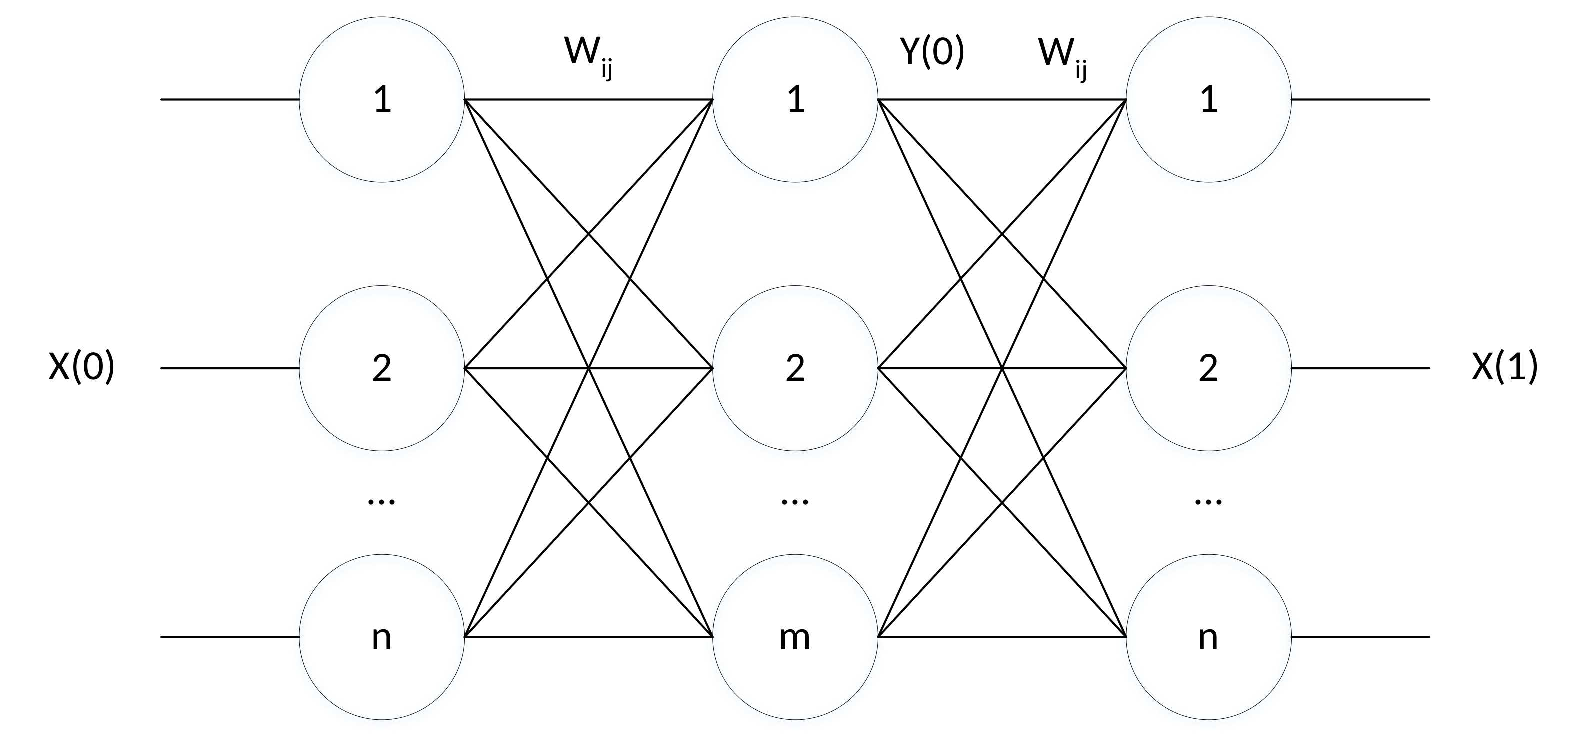
\includegraphics[width=0.9\textwidth]{man-source/images/ch2/pic2-1.pdf}
  \caption{Развернутое представление RBM}
  \label{fig:pic2_1}
\end{figure}

Представим сэмплирование Гиббса, используя развернутое представление RBM (рисунок~\ref{fig:pic2_2}).

\begin{figure}[H]
  \centering
  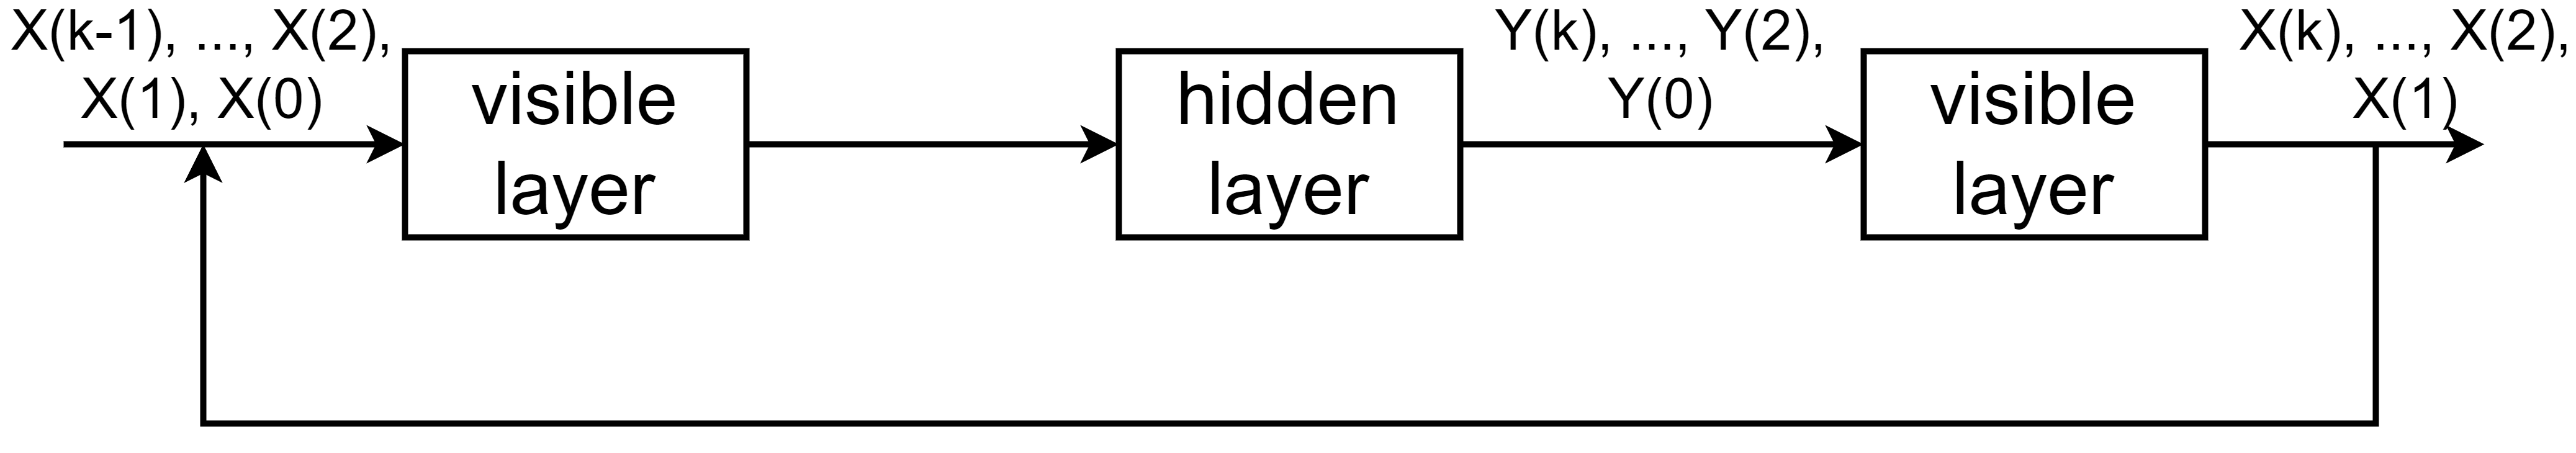
\includegraphics[width=\textwidth]{man-source/images/ch2/pic2-2.png}
  \caption{Сэмплирование Гиббса}
  \label{fig:pic2_2}
\end{figure}

Сэмплирование Гиббса заключается в следующей процедуре. Пусть $x(0)$ -- входной вектор, который поступает на видимый слой в момент времени $t=0$. Тогда выходные значения нейронов скрытого слоя будут определяться следующим образом:

\begin{equation}
    y_j(0)=F(S_j(0)),
\end{equation}

\begin{equation}
    S_j(0)=\sum_i w_{ij}x_i(0)+T_j.
\end{equation}

Инверсный (последний) слой  реконструирует входной вектор на основе данных со скрытого слоя и текущего значения настраиваемых параметров (порогов видимого слоя и матрицы весов). В результате получается восстановленный вектор $x(1)$ в момент времени $t=1$:

\begin{equation}
    x_i(1)=F(S_i(1)),
\end{equation}

\begin{equation}
    S_i(1)=\sum_j w_{ij}y_j(0)+T_i.
\end{equation}

Затем вектор $x(1)$ поступает на видимый слой, и вычисляются выходные значения нейронов скрытого слоя: 

\begin{equation}
    y_j(1)=F(S_j(1)),
\end{equation}

\begin{equation}
    S_j(1)=\sum_i w_{ij}x_i(1)+T_j.
\end{equation}

Продолжая данный процесс, можно получить на шаге k следующие выражения:

\begin{equation*}		
    y_j(k)=F(S_j(k)),\ S_j(k)=\sum_i w_{ij}x_i(k)+T_j,
\end{equation*}

\begin{equation*}		
    x_i(k)=F(S_i(k)),\ S_i(k)=\sum_j w_{ij}y_j(k-1)+T_i.
\end{equation*}

\section{Вывод правил предобучения} 

Хинтоном была предложена энергетическая модель, базирующаяся на идее максимизации функции правдоподобия распределения входных данных $P(x)$. Вывод классических правил обучения был приведен в главе I. Основываясь на идее использования ограниченной машины Больцмана в качестве вспомогательной модели для проведения предобучения, было предложено использование двух разных критериев для ее обучения \cite{4-A}. Первый критерий основывается на минимизации среднеквадратичной ошибки (MSE), а второй -- на минимизации кросс-энтропийной функции ошибки.

Покажем, что применение различных критериев минимизации позволяет, тем не менее, получить одинаковые правила обучения.

\subsection{Критерий MSE}

В случае использования в качестве критерия обучения MSE основной целью обучения ограниченной машины Больцмана является минимизация суммарной среднеквадратичной ошибки реконструкции данных на скрытом и видимом (восстанавливающем) слое, которая в случае CD-k определяется следующим образом:	

\begin{equation*}	
    E_s(k)=\frac{1}{2L}\Bigg(\sum_{l=1}^L\sum_{j=1}^m\sum_{p=1}^k (y_j^l(p)-y_j^l(p-1))^2+\sum_{l=1}^L\sum_{i=1}^n\sum_{p=1}^k (x_i^l(p)-x_i^l(p-1))^2\Bigg),
\end{equation*}
где \textit{k} определяет параметр процедуры сэмплирования Гиббса,\\
\textit{n} -- количество нейронов в видимом слое,\\
\textit{m} -- количество нейронов в скрытом слое,\\
\textit{L} -- размерность обучающей выборки.

В случае CD-1  суммарная среднеквадратичная ошибка:

\begin{equation}
    E_s(1)=\frac{1}{2L}\Bigg(\sum_{l=1}^L\sum_{j=1}^m (y_j^l(1)-y_j^l(0))^2+\sum_{l=1}^L\sum_{i=1}^n (x_i^l(1)-x_i^l(0))^2\Bigg).
\end{equation}

Как следует из приведенных выше выражений, ошибка состоит из двух частей: ошибки восстановления информации на видимом и скрытом слоях, то есть может быть представлена в следующем виде:
\begin{equation}
	\label{mse_rbm_criteria}
	E_s(k) = E_h(k) + E_v(k),
\end{equation}
где

\begin{equation}
	E_h(k) = \frac{1}{2L}\sum_{l=1}^L\sum_{j=1}^m\sum_{p=1}^k (y_j^l(p)-y_j^l(p-1))^2,
\end{equation}

\begin{equation}
	E_v(k) = \frac{1}{2L}\sum_{l=1}^L\sum_{i=1}^n\sum_{p=1}^k (x_i^l(p)-x_i^l(p-1))^2.
\end{equation}

Найдем правила обучения, соответствующие критерию \ref{mse_rbm_criteria} и докажем их эквивалентность классическим правилам обучения RBM при выполнении некоторых специальных условий.

\textbf{Теорема 1}. Максимизация функции правдоподобия распределения данных $P(x)$ в пространстве синаптических связей ограниченной машины Больцмана эквивалентна минимизации суммарной квадратичной ошибки сети в том же пространстве при использовании линейных нейронов.

\textbf{Доказательство}: Рассмотрим последовательное обучение RBM, когда модификация синаптических связей происходит после подачи каждого входного образа на сеть (онлайн-обучение). В соответствии с методом градиентного спуска для минимизации суммарной квадратичной ошибки сети, синаптические связи должны изменяться следующим образом:	

\begin{equation}
w_{ij}(t+1)=w_{ij}(t)-\alpha\frac{\partial E}{\partial w_{ij}(t)},
\end{equation}		

\begin{equation}
T_{i}(t+1)=T_{i}(t)-\alpha\frac{\partial E}{\partial T_{i}(t)},
\end{equation}		

\begin{equation}
T_{j}(t+1)=T_{j}(t)-\alpha\frac{\partial E}{\partial T_{j}(t)}.
\end{equation}

В случае CD-k квадратичная ошибка $E$ для одного образа:

\begin{equation*}
E=\frac{1}{2}\sum_{j=1}^m\sum_{p=1}^k (y_j(p)-y_j(p-1))^2+\frac{1}{2}\sum_{i=1}^n\sum_{p=1}^k (x_i(p)-x_i(p-1))^2.
\end{equation*}

Тогда
\begin{multline*}
    \frac{\partial E}{\partial w_{ij}}=\frac{\partial E}{\partial y_j(p)}\frac{\partial y_j(p)}{\partial S_j(p)}\frac{\partial S_j(p)}{\partial w_{ij}}+\frac{\partial E}{\partial x_i(p)}\frac{\partial x_i(p)}{\partial S_i(p)}\frac{\partial S_i(p)}{\partial w_{ij}}=\\=\sum_{p=1}^k (y_j(p)-y_j(p-1))x_i(p)F'(S_j(p))+\\+\sum_{p=1}^k (x_i(p)-x_i(p-1))y_j(p-1)F'(S_i(p)).
\end{multline*}

Если ограниченная машина Больцмана использует линейные нейроны с линейной функцией активации, то

\begin{equation*}
    \frac{\partial S_i(p)}{\partial w_{ij}}=F'(S_i(p))=\frac{\partial S_j(p)}{\partial w_{ij}}=F'(S_j(p))=1.
\end{equation*}

Тогда

\begin{equation*}
    \frac{\partial E}{\partial w_{ij}}=\sum_{p=1}^k (y_j(p)x_i(p)-y_j(p-1)x_i(p-1))=y_j(k)x_i(k)-y_j(0)x_i(0).
\end{equation*}

В результате можно получить CD-k правило обучения RBM:

\begin{equation*}
    w_{ij}(t+1)=w_{ij}(t)+\alpha(x_i(0)y_j(0)-x_i(k)y_j(k)).
\end{equation*}

Аналогичным образом для пороговых значений:

\begin{equation*}
\begin{aligned}
    T_{j}(t+1)=T_{j}(t)+\alpha(y_j(0)-y_j(k)),\\
    T_{i}(t+1)=T_{i}(t)+\alpha(x_i(0)-x_i(k)).
\end{aligned}
\end{equation*}

Как видно последние выражения совпадают с классическим правилом обучения ограниченной машины Больцмана для CD-k. Отсюда следует, что для линейной RBM максимизация функции правдоподобия распределения данных $P(x)$ эквивалентна минимизации суммарной квадратичной ошибки сети. Теорема доказана.

\textbf{Следствие 1.1}. Линейная ограниченная машина Больцмана c точки зрения обучения эквивалентна автоассоциативной нейронной сети при использовании в ней при обучении сэмплирования Гиббса.

\textbf{Следствие 1.2}. Для нелинейной ограниченной машины Больцмана правило модификации синаптических связей в случае CD-k будет следующим:
\begin{multline*}
    w_{ij}(t+1)=w_{ij}(t)-\\-\alpha\Bigg(\sum_{p=1}^k (y_j(p)-y_j(p-1))x_i(p)F'(S_j(p))+(x_i(p)-x_i(p-1))y_j(p-1)F'(S_i(p))\Bigg),
\end{multline*}

\begin{equation*}
\begin{aligned}
    T_i(t+1)=T_i(t)-\alpha\left(\sum_{p=1}^k (x_i(p)-x_i(p-1))F'(S_i(p))\right),\\
    T_j(t+1)=T_j(t)-\alpha\left(\sum_{p=1}^k (y_j(p)-y_j(p-1))F'(S_j(p))\right).
\end{aligned}
\end{equation*}

\textbf{Следствие 1.3}. Для нелинейной ограниченной машины Больцмана правило модификации синаптических связей в случае CD-1 будет следующим:	
\begin{equation*}
    w_{ij}(t+1)=w_{ij}(t)-\alpha((y_j(1)-y_j(0))F'(S_j(1))x_i(1)+(x_i(1)-x_i(0))F'(S_i(1))y_j(0)),
\end{equation*}

\begin{equation*}
    T_i(t+1)=T_i(t)-\alpha(x_i(1)-x_i(0))F'(S_i(1)),
\end{equation*}

\begin{equation*}
    T_j(t+1)=T_j(t)-\alpha(y_j(1)-y_j(0))F'(S_j(1)).  
\end{equation*}

При использовании группового обучения (batch learning), метод градиентного спуска примет следующий вид:

\begin{equation}
    w_{ij}(t+1)=w_{ij}(t)-\alpha\frac{\partial E_s}{\partial w_{ij}(t)},
\end{equation}

\begin{equation}
    T_{i}(t+1)=T_{i}(t)-\alpha\frac{\partial E_s}{\partial T_{i}(t)},
\end{equation}

\begin{equation}
    T_{j}(t+1)=T_{j}(t)-\alpha\frac{\partial E_s}{\partial T_{j}(t)}.
\end{equation}

\textbf{Теорема 2}. При использовании  CD-k для нелинейной ограниченной машины Больцмана в случае группового обучения правило модификации синаптических связей определяется на основе следующих выражений:
\begin{multline*}
    w_{ij}(t+1)=w_{ij}(t)-\\-\frac{\alpha}{L}\Bigg(\sum_{l=1}^L\sum_{p=1}^k (y_j^l(p)-y_j^l(p-1))x_i^l(p)F'(S_j^l(p))+(x_i^l(p)-x_i^l(p-1))y_j^l(p-1)F'(S_i^l(p))\Bigg),
\end{multline*}

\begin{equation*}
    T_{i}(t+1)=T_{i}(t)-\frac{\alpha}{L}\left(\sum_{l=1}^L\sum_{p=1}^k (x_i^l(p)-x_i^l(p-1))F'(S_i^l(p))\right),
\end{equation*}

\begin{equation*}
    T_{j}(t+1)=T_{j}(t)-\frac{\alpha}{L}\left(\sum_{l=1}^L\sum_{p=1}^k (y_j^l(p)-y_j^l(p-1))F'(S_j^l(p))\right).
\end{equation*}

Процесс доказательства данной теоремы является аналогичным доказательству теоремы 1.

\textbf{Следствие 2.1}. При использовании  CD-1 для нелинейной ограниченной машины Больцмана в случае группового обучения правило модификации синаптических связей определяется на основе следующих выражений:

\begin{multline*}
    w_{ij}(t+1)=w_{ij}(t)-\\-\frac{\alpha}{L}\left(\sum_{l=1}^L (y_j^l(1)-y_j^l(0))x_i^l(1)F'(S_j^l(1))+(x_i^l(1)-x_i^l(0))y_j^l(0)F'(S_i^l(1))\Bigg)\right.,
\end{multline*}

\begin{equation*}
    T_i(t+1)=T_i(t)-\frac{\alpha}{L}\left(\sum_{l=1}^L (x_i^l(1)-x_i^l(0))F'(S_i^l(1))\right),
\end{equation*}

\begin{equation*}
    T_j(t+1)=T_j(t)-\frac{\alpha}{L}\left(\sum_{l=1}^L (y_j^l(1)-y_j^l(0))F'(S_j^l(1))\right).
\end{equation*}

\textbf{Следствие 2.2}. При использовании  CD-k для линейной ограниченной машины Больцмана в случае группового обучения правило модификации синаптических связей определяется на основе следующих выражений:

\begin{equation*}
    w_{ij}(t+1)=w_{ij}(t)+\frac{\alpha}{L}\sum_{l=1}^L (x_i^l(0)y_j^l(0)-x_i^l(k)y_j^l(k)),
\end{equation*}

\begin{equation*}
    T_{i}(t+1)=T_{i}(t)+\frac{\alpha}{L}\sum_{l=1}^L (x_i^l(0)-x_i^l(k)),
\end{equation*}

\begin{equation*}
    T_{j}(t+1)=T_{j}(t)+\frac{\alpha}{L}\sum_{l=1}^L (y_j^l(0)-y_j^l(k)).
\end{equation*}

\textbf{Следствие 2.3}. При использовании  CD-1 для линейной ограниченной машины Больцмана в случае группового обучения правило модификации синаптических связей определяется на основе следующих выражений:

\begin{equation*}
    w_{ij}(t+1)=w_{ij}(t)+\frac{\alpha}{L}\sum_{l=1}^L (x_i^l(0)y_j^l(0)-x_i^l(1)y_j^l(1)),
\end{equation*}

\begin{equation*}
    T_{i}(t+1)=T_{i}(t)+\frac{\alpha}{L}\sum_{l=1}^L (x_i^l(0)-x_i^l(1)),
\end{equation*}

\begin{equation*}
    T_{j}(t+1)=T_{j}(t)+\frac{\alpha}{L}\sum_{l=1}^L (y_j^l(0)-y_j^l(1)).
\end{equation*}

Таким образом, получены правила обучения для ограниченной машины Больцмана, которые базируются на минимизации квадратичной ошибки восстановления информации на видимом и скрытом слоях.  Предложенный метод позволяет учитывать нелинейную природу нейронных элементов. Показано, что классические выражения для обучения ограниченной машины являются частным случаем предложенного метода. Доказана теорема об эквивалентности максимизации функции правдоподобия распределения входных данных $P(x)$ и минимизации суммарной квадратичной ошибки сети в одном и том же пространстве синаптических связей для линейной ограниченной машины Больцмана. 

% Впервые подход был представлен в \cite{n9} для случая CD-1 и в \cite{Golovko2015a, Golovko2015b} для случая CD-k.

\subsection{Критерий СЕ}

В случае CD-k кросс-энтропийная функция ошибки для видимого слоя определяется следующим образом:

\begin{equation*}
	CE_v(k) = -\frac{1}{L}\sum_{l=1}^L \sum_{p=1}^k \sum_{i=1}^n x_i^l(p-1)\log(x_i^l(p))+(1-x_i^l(p-1)\log(1-x_i^l(p)),
\end{equation*}
где $L$ -- размер обучающей выборки,\\
$k$ -- параметр процедуры сэмплирования,\\
$n$ -- количество нейронов на видимом слое.

Аналогично для скрытого слоя:

\begin{equation*}
	CE_h(k) = -\frac{1}{L}\sum_{l=1}^L \sum_{p=1}^k \sum_{j=1}^m y_j^l(p-1)\log(y_j^l(p))+(1-y_j^l(p-1)\log(1-y_j^l(p)),
\end{equation*}
где $m$ -- количество нейронов на скрытом слое.

Общая функция определяется как сумма кросс-энтропийных функций ошибки видимого и скрытого слоев:

\begin{equation}
	CE_s(k) = CE_h(k)+CE_v(k).
\end{equation}

Докажем следующую теорему.

\textbf{Теорема 3}. Максимизация функции правдоподобия распределения входных данных $P(x)$ эквивалентна минимизации кросс-энтропийной целевой функции $CE_s(k)$ в одном и том же пространстве синаптических весов ограниченной машины Больцмана (случай $k=1$).

\textbf{Доказательство}. В случае CD-1 кросс-энтропийная функция для одного обучающего примера будет иметь следующий вид:

\begin{multline}
	CE(1) = -\sum_{i=1}^n (x_i(0)\log(x_i(1))+(1-x_i(0))\log(1-x_i(1)))-\\-\sum_{j=1}^m ( y_j(0)\log(y_j(1))+(1-y_j(0))\log(1-y_j(1))) = \\ = CE_v(1)+CE_h(1).
\end{multline}

Найдем частные производные кросс-энтропийной функции по весовым элементам. Получим

\begin{equation*}
	\frac{\partial CE(1)}{\partial w_{ij}} = \frac{\partial CE_v(1)}{\partial w_{ij}} + \frac{\partial CE_h(1)}{\partial w_{ij}}.
\end{equation*}

Тогда

\begin{multline*}
	\frac{\partial CE_v(1)}{\partial w_{ij}} = -\frac{x_i(0)}{x_i(1)}x_i(1)(1-x_i(1))y_j(0)+\frac{1-x_i(0)}{1-x_i(1)}x_i(1)(1-x_i(1))y_j(0) = \\ = -x_i(0)(1-x_i(1))y_j(0)+(1-x_i(0))x_i(1)y_j(0)=\\=-x_i(0)y_j(0)+x_i(0)x_i(1)y_j(0)+x_i(1)y_j(0)-x_i(0)x_i(1)y_j(0)=\\=-x_i(0)y_j(0)+x_i(1)y_j(0) 
\end{multline*}

и

\begin{multline*}
	\frac{\partial CE_h(1)}{\partial w_{ij}} = -y_j(0)(1-y_j(1))x_i(1)+(1-y_j(0))y_j(1)x_i(1) = \\ = -y_j(0)x_i(0)+y_j(0)y_j(1)x_i(1)+y_j(1)x_i(1)-y_j(0)y_j(1)x_i(1) = \\ = -y_j(0)x_i(1)+y_j(1)x_i(1). 
\end{multline*}

Окончательно получим

\begin{multline*}
	\frac{\partial CE(1)}{\partial w_{ij}} = \frac{\partial CE_v(1)}{\partial w_{ij}} + \frac{\partial CE_h(1)}{\partial w_{ij}} = \\ = -x_i(0)y_j(0)+x_i(1)y_j(0) -y_j(0)x_i(1)+y_j(1)x_i(1) = x_i(1)y_j(1) - x_i(0)y_j(0).
\end{multline*}

Аналогично, для пороговых элементов имеем:

\begin{multline*}
	\frac{\partial CE(1)}{\partial T_i} = \frac{\partial CE_v(1)}{\partial T_i} = -\frac{x_i(0)}{x_i(1)}x_i(1)(1-x_i(1))+\frac{1-x_i(0)}{1-x_i(1)}x_i(1)(1-x_i(1)) = \\ = -x_i(0) + x_i(0)x_i(1)+x_i(1)-x_i(0)x_i(1) = x_i(1)-x_i(0);
\end{multline*}

\begin{multline*}
	\frac{\partial CE(1)}{\partial T_j} = \frac{\partial CE_h(1)}{\partial T_j} = -y_j(0)(1-y_j(1)) + (1-y_j(0))y_j(1) = \\ = -y_j(0) + y_j(0)y_j(1) + y_j(1) - y_j(0)y_j(1) = y_j(1) - y_j(0).
\end{multline*}

Теорема доказана. 

Рассматривая более общий случай CD-k, можно доказать следующую теорему.

\textbf{Теорема 4}. Максимизация функции правдоподобия распределения входных данных $P(x)$ эквивалентна минимизации кросс-энтропийной целевой функции $CE_s(k)$ в одном и том же пространстве синаптических весов ограниченной машины Больцмана (случай произвольного $k$).

\textbf{Доказательство}. В случае CD-k кросс-энтропийная функция для одного обучающего примера будет иметь следующий вид:

\begin{multline}
	CE_s(k) = -\sum_{p=1}^k \sum_{i=1}^n (x_i(p-1)\log(x_i(p)) + (1-x_i(p-1))\log(1-x_i(p)))-\\-\sum_{p=1}^k \sum_{j=1}^m (y_j(p-1)\log (y_j(p))+(1-y_j(p-1))\log(1-y_j(p))) = \\ = CE_v(k) + CE_h(k).
\end{multline}

Как и в случае CD-1 находим соответствующие частные производные по весовым и пороговым элементам. Имеем:

\begin{equation*}
	\frac{\partial CE_s(k)}{\partial w_{ij}}= \frac{\partial CE_v(k)}{\partial w_{ij}} + \frac{\partial CE_h(k)}{\partial w_{ij}}.
\end{equation*}

Причем

\begin{multline*}
	\frac{\partial CE_v(k)}{\partial w_{ij}} = \\ = -\sum_{p=1}^k (x_i(p-1)(1-x_i(p))y_j(p-1)-(1-x_i(p-1))x_i(p)y_j(p-1))=\\=-\sum_{p=1}^k (x_i(p-1)y_j(p-1)-x_i(p-1)x_i(p)y_j(p-1)-\\-x_i(p)y_j(p-1)+x_i(p-1)x_i(p)y_j(p-1)) = \\ = \sum_{p=1}^{k} (x_i(p)y_j(p-1)-x_i(p-1)y_j(p-1))
\end{multline*}

и

\begin{multline*}
	\frac{\partial CE_h(k)}{\partial w_{ij}} = \\ = -\sum_{p=1}^k (y_j(p-1)(1-y_j(p))x_i(p)-(1-y_j(p-1))y_j(p)x_i(p)) = \\ = -\sum_{p=1}^{k} (y_j(p-1)x_i(p)-y_j(p-1)y_j(p)x_i(p)-\\-y_j(p)x_i(p)+y_j(p-1)y_j(p)x_i(p)) = \\ = \sum_{p=1}^{k} (x_i(p)y_j(p)-x_i(p)y_j(p-1)).
\end{multline*}

А значит

\begin{multline*}
	\frac{\partial CE_s(k)}{\partial w_{ij}} = \sum_{p=1}^{k}(y_j(p)x_i(p)-x_i(p-1)y_j(p-1)) = \\ = y_j(1)x_i(1)-x_i(0)y_j(0)+x_i(2)y_j(2)-x_i(1)y_j(1)+\dots+\\+x_i(k)y_j(k)-x_i(k-1)y_j(k-1)=\\=x_i(k)y_j(k)-x_i(0)y_j(0).
\end{multline*}

Аналогично для пороговых элементов:

\begin{multline*}
	\frac{\partial CE_s(k)}{\partial T_i} = \frac{\partial CE_v(k)}{\partial T_i} =\\= -\sum_{p=1}^k (x_i(p-1)(1-x_i(p))-(1-x_i(p-1))x_i(p)) =\\= \sum_{p=1}^k (x_i(p) - x_i(p-1)) = x_i(1)-x_i(0)+x_i(2) - x_i(1) +\dots+x_i(k)-x_i(k-1) =\\= x_i(k)-x_i(0);
\end{multline*}

\begin{multline*}
	\frac{\partial CE_s(k)}{\partial T_j} = \frac{\partial CE_h(k)}{\partial T_j} =\\= -\sum_{p=1}^k (y_j(p-1)(1-y_j(p))-(1-y_j(p-1))y_j(p)) =\\= \sum_{p=1}^k (y_j(p) - y_j(p-1)) = y_j(1)-y_j(0)+y_j(2) - y_j(1) +\dots+y_j(k)-y_j(k-1) =\\= y_j(k)-y_j(0).
\end{multline*}

Теорема доказана.

Из доказанных теорем 3 и 4 следует, что правила обучения ограниченной машины Больцмана могут быть получены более простым путем, чем при использовании традиционного подхода, основанного на применении функции энергии. Произведя минимизацию кросс-энтропийной функции и применяя простые итерации сэмплирования Гиббса, мы получили классические линейные правила обучения RBM.

Таким образом, на основании доказанных теорем 1-4 можно сформулировать общую теорему.

\textbf{Теорема 5}. Максимизация функции правдоподобия распределения входных данных $P(x)$ эквивалентна минимизации кросс-энтропийной функции и специальному случаю минимизации среднеквадратичной ошибки в одном и том же пространстве синаптических весов ограниченной машины Больцмана:

\begin{equation}
	\max(\ln P(x)) = \min(CE_s) = \min(E_s).
\end{equation}

Теорема 5 обобщает предыдущие результаты. Как следует из этой теоремы, использование различных критериев обучения приводит к тем же самым правилам. Поэтому сущность неконтролируемого обучения для ограниченной машины Больцмана одинакова, даже если используются различные целевые функции. Максимизация функции правдоподобия и минимизация кросс-энтропийной функции ошибки приводит к линейному представлению нейронных элементов в терминах минимизации функции MSE. Необходимо отметить, что, применяя критерий MSE, мы учитываем также нелинейное представление нейронных элементов. Таким образом, очевидное преимущество в использовании MSE в качестве функции ошибок перед применением функции максимального правдоподобия и кросс-энтропийной функции в том, что при использовании MSE могут быть получены как линейные, так и нелинейные правила обучения.

В дальнейшем для идентификации предлагаемого подхода будем использовать аббревиатуру REBA (Reconstruction Error-Based Approach). Классический метод будем называть C-RBM (Classic Restricted Boltzmann Machine Training).

\section{Предобучение сверточных слоев}

Выполнение предобучения сверточных слоев имеет особое значение при решении задач компьютерного зрения в силу эффективности таких слоев при обработке визуальной информации, представленной с помощью отдельных изображений и видео.

Отметим, что преобразования, выполняемые над сверточными слоями при обучении, идентичны преобразованиям для полносвязных слоев. 
Отличие заключается в операции <<развертки>> (deconvolution), которая используется на этапе предобучения при реконструкции активности видимых нейронов и на этапе тонкой настройки для метода обратного распространения при вычислении ошибок на скрытых слоях сети. Эта операция применяется в сверточных нейронных сетях для повышения частоты дискретизации.
Рассмотрим визуальное представление операции свертки для случая карт 3Х3 и 2Х2 (рисунок \ref{fig:convolution}).

\begin{figure}[H]
  \centering
  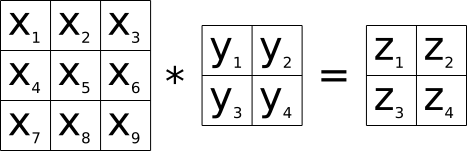
\includegraphics[width=0.5\textwidth]{man-source/images/ch2/pic2-4.png}
  \caption{Операция свертки}
  \label{fig:convolution}
\end{figure}

Сверточный слой с одним ядром может быть представлен в виде разряженного слоя, а операция <<развертки>> -- слоем, полученным применением симметричного преобразования относительно разряженного. При этом полученная сеть представляет собой автоэнкодер с симметричными связями относительно скрытого слоя (рисунок \ref{fig:convolution_autoencoder}).

На основании данного представления могут быть получены формулы для выполнения <<развертки>>:

\begin{equation*}
	x'_1 = z_1y_1		
	\end{equation*}
	\begin{equation*}
	x'_2 = z_1y_2+z_2y_1
	\end{equation*}
	\begin{equation*}
	x'_3 = z_2y_2
	\end{equation*}
	\begin{equation*}
	x'_4 = z_1y_3 + z_3y_1
	\end{equation*}
	\begin{equation*}
	x'_5 = z_1y_4 + z_2y_3 + z_3y_2 + z_4y_1
	\end{equation*}
	\begin{equation*}
	x'_6 = z_2y_4 + z_4y_2
	\end{equation*}
	\begin{equation*}
	x'_7 = z_3y_3
	\end{equation*}
	\begin{equation*}
	x'_8 = z_3y_4 + z_4y_3
	\end{equation*}		
	\begin{equation*}
	x'_9 = z_4y_4
	\end{equation*}	

\begin{figure}[H]
  \centering
  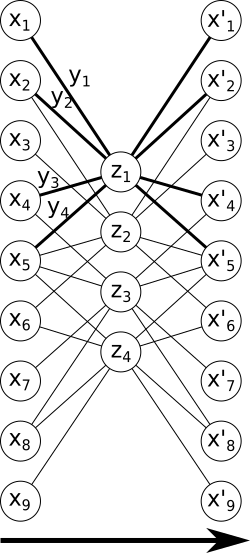
\includegraphics[width=0.4\textwidth]{man-source/images/ch2/pic2-5.png}
  \caption{Разряженный автоэнкодер операции свертки}
  \label{fig:convolution_autoencoder}
\end{figure}

Сама операция <<развертки>> представлена на рисунке \ref{fig:deconvolution}.

\begin{figure}[H]
  \centering
  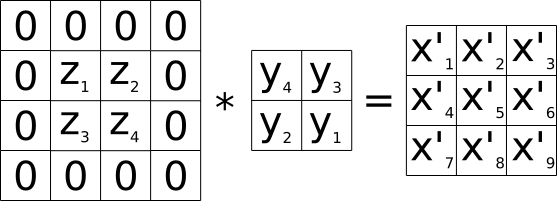
\includegraphics[width=0.6\textwidth]{man-source/images/ch2/pic2-6.png}
  \caption{Операция <<развертки>>}
  \label{fig:deconvolution}
\end{figure}

Введя операции матричного поворота на 180 градусов и заполнения нулями границ матрицы (padding), можно получить следующие общие формулы для выполнения <<развертки>> (рисунок \ref{fig:deconvolution_formula}).

\begin{figure}[H]
  \centering
  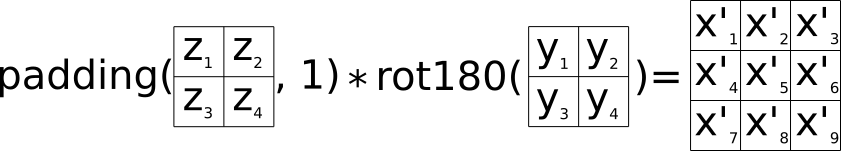
\includegraphics[width=0.9\textwidth]{man-source/images/ch2/pic2-9.png}
  \caption{Формула <<развертки>>}
  \label{fig:deconvolution_formula}
\end{figure}

Введем условное обозначение для операции <<развертки>> -- $\circledast$.

Применяя полученную формулу для выполнения <<развертки>>, можно осуществлять процедуру CD на сверточных слоях ГНС, которые в этом случае рассматриваются как сверточные ограниченные машины Больцмана (CRBM). 

Рассмотрим формулы для получения необходимых карт признаков для расчета градиента изменения параметров слоя в случае использования процедуры CD-1: 

\begin{equation*}
    y_j(0) = F(x_i(0) * w_{ij} + T_j),
\end{equation*}

\begin{equation*}
    x_i(1) = F(y_j(0) \circledast w_{ij} + T_i),
\end{equation*}

\begin{equation*}
    y_j(1) = F(x_i(1) * w_{ij} + T_j),
\end{equation*}
где $w_{ij}$ -- $i$-тый компонент $j$-того ядра свертки,\\
$x_i(0)$ -- $i$-тый компонент входной карты признаков,\\
$T_j$ -- пороговый элемент $j$-того нейрона скрытого слоя,\\
$y_j(0)$ -- $j$-тый компонент выходной карты признаков,\\
$x_i(1)$ -- $i$-тый компонент реконструированной входной карты признаков,\\
$T_i$ -- пороговый элемент $i$-того нейрона видимого слоя,\\
$y_j(1)$ -- $j$-тый компонент реконструированной выходной карты признаков.

Классические правила обучения RBM могут быть переформулированы для случая CRBM (CD-1, последовательное обучение): 

\begin{equation*}
		w_{ij}(t+1)=w_{ij}(t)+\alpha(x_i(0) * y_j(0)-x_i(1) * y_j(1)),
\end{equation*} 

\begin{equation*}	
		T_i(t+1)=T_i(t)+\alpha(x_i(0)-x_i(1)),
\end{equation*} 

\begin{equation*}		
		T_j(t+1)=T_j(t)+\alpha(y_j(0)-y_j(1)).
\end{equation*}
% где $\circledast$ обозначает операцию свертки.

В соответствии с предлагаемым методом, правила обучения могут быть переформулированы следующим образом (CD-1, последовательное обучение):

\begin{multline*}
    w_{ij}(t+1)=w_{ij}(t)-\alpha((y_j(1)-y_j(0))F'(S_j(1)) * x_i(1)+\\(x_i(1)-x_i(0))F'(S_i(1)) * y_j(0)),    
\end{multline*}
\begin{equation*}
    T_i(t+1)=T_i(t)-\alpha(x_i(1)-x_i(0))F'(S_i(1)),
\end{equation*}
\begin{equation*}
    T_j(t+1)=T_j(t)-\alpha(y_j(1)-y_j(0))F'(S_j(1)).  
\end{equation*}

Аналогичным образом могут быть получены правила для CD-\textit{k} случая процедуры обучения и группового случая.

Таким образом, для глубокой сверточной нейронной сети, содержащей слои разных типов (полносвязные и сверточные) возможно сочетание нескольких вариантов обучения -- с представлением в виде CRBM (для сверточных слоев) и в виде RBM (для полносвязных).  

\section{Метод редуцирования параметров}
Известно, что полносвязные нейронные сети обладают определенной степенью избыточности. Полносвязный слой в сравнении со сверточным содержит большее количество настраиваемых параметров, однако в задачах компьютерного зрения сверточные нейронные сети показывают существенно лучшие результаты по обобщающей способности, чем полносвязные. Таким образом, очевидно, что в полносвязных сетях при большем количестве настраиваемых параметров, они используются менее оптимально. Можно предположить, что указанные <<избыточные>> параметры могут быть исключены без существенного ухудшения эффективности работы модели. Важный вопрос, возникающий при выполнении такой операции редуцирования, касается самого алгоритма отсеивания малоинформативных параметров.

К основным методам компрессии (сжатия) нейросетевых моделей на настоящий момент относятся:
\begin{easylistNum}
	& прунинг -- pruning (\cite{wang2019pruning}, \cite{xu2020});
	& квантизация -- quantization \cite{hubara2016quantized};
	& дистилляция -- distillation \cite{Hinton2015DistillingTK};
	& матричная факторизация низкого ранга -- low-rank matrix factorization \cite{Sainath2013}.
\end{easylistNum}

\textit{Прунинг} позволяет удалить часть связей и нейронов (в зависимости от выполняемой техники редуцирования), что уменьшает структурную избыточность <<тяжелых>> глубоких нейросетевых моделей.
По типу выполняемой техники прунинга выделяют:

\begin{easylist}
	& прунинг связей;
	& прунинг нейронов или фильтров (в зависимости от типа слоя -- полносвязного или сверточного);
	& прунинг слоев.
\end{easylist}

\textit{Квантизация} используется для физического уменьшения памяти, занимаемой моделью. В этом подходе осуществляется редуцирование типа данных, используемого для хранения параметров нейросетевой модели (например, осуществляется переход от 32-битного к 16-битному или 8-битному представлению типа).

\textit{Дистилляция} основывается на возможности использования более <<тяжелых>> моделей для обучения моделей меньшего размера. В этом случае обученная модель-учитель генерирует примеры, которые используются для обучения модели-ученика. Размер такой модели-ученика может быть существенно меньше первоначальной сети. По разновидностям выделяют следующие типы дистилляции:

\begin{easylist}
	& офлайн-дистилляция (применяется последовательное обучение модели-учителя, затем -- модели-ученика);
	& онлайн-дистилляция (применяется одновременное обучение модели-учителя и модели-ученика);
	& самодистилляция (в качестве модели-учителя и модели-ученика выступает одна модель).
\end{easylist}

Наконец, \textit{матричная факторизация низкого ранга} позволяет осуществить декомпозицию матрицы весовых коэффициентов большого размера на совокупность матриц меньшего размера. Применение данного подхода помогает уменьшить память, занимаемую моделями и ускорить время работы модели. К недостаткам метода относят его вычислительную сложность.
% Редуцирование параметров нейросетевой модели позволяет добиться уменьшения количества настраиваемых параметров, что может быть актуальным при применении нейронных сетей на устройствах с ограниченными аппаратными возможностями (одноплатные компьютеры, мобильные телефоны и т.д.). Применение при этом специальных методик для хранения разряженных матриц позволяет ускорить работу архитектуры. Важно, чтобы при этом сеть сохраняла свою обобщающую способность.

Предлагаемый алгоритм редуцирования связей НС основывается на прунинге, но имеет модификацию, которая заключается в наличии этапа неконтролируемого предобучения на основе RBM.

Рассмотрим подход для редуцирования связей полносвязной нейронной сети, основанный на использовании предобучения. Первый и четвертый этапы данной процедуры аналогичны этапам выполнения предобучения типа II, описанного в главе I. В ходе выполнения дополнительных этапов 2 и 3 формируются разряженные связи между входными и выходными нейронными элементами слоя и уменьшается его размерность за счет удаления части нейронных элементов, которые не используются при <<тонкой настройке>> и дальнейшей эксплуатации нейросетевой модели (рисунок~\ref{fig:pic2_3}):
\begin{easylistNum}
    & неконтролируемое предобучение НС с использованием <<жадного>> алгоритма, начиная с первого слоя. Параметры каждого слоя, представленные весовыми и пороговыми коэффициентами, настраиваются в соответствии с правилами обучения ограниченной машины Больцмана;
    & <<обнуление>> весовых коэффициентов слоев нейронной сети, абсолютные значения которых не превышают некоторый заданный порог $t > 0$. Иначе говоря, параметры со значениями, попадающими в интервал $[-t, t]$, не изменяются при дальнейшем обучении;
    & архитектурная реконфигурация нейронной сети, в ходе которой удаляются нейроны, не участвующие в формировании выходной активности сети (нейроны, имеющие нулевые векторы весовых коэффициентов или, в случае использования сверточных слоев, нейроны, имеющие нулевые ядра свертки). Реконфигурация выполняется в соответствии со следующими правилами:\\
        для каждого \textit{i}-того слоя НС, кроме первого и последнего:
        \begin{itemize}
            \item если вектор-столбец $j$ матрицы весовых коэффициентов $W_i$ нулевой, то удалить $j$-тый вектор-столбец из $W_i$ и удалить $j$-тую вектор-строку из $W_{i+1}$;
            \item если вектор-строка $k$ матрицы весовых коэффициентов $W_i$ нулевая, то удалить $k$-тую вектор-строку из $W_i$ и удалить $k$-тый вектор-столбец из матрицы $W_{i-1}$;
        \end{itemize}
    & <<тонкая настройка>> параметров слоев полученной НС с упрощенной архитектурой, например, методом обратного распространения ошибки.
\end{easylistNum}

Этап 2 может дополнительно включать уплотнение для разреженной  матрицы параметров в целях достижения более компактного представления весовых коэффициентов.

Таким образом, в процессе реализации данного алгоритма осуществляется отсеивание весовых коэффициентов, значениями которых можно пренебречь в соответствии с некоторым заданным порогом.

\begin{figure}[H]
  \centering
  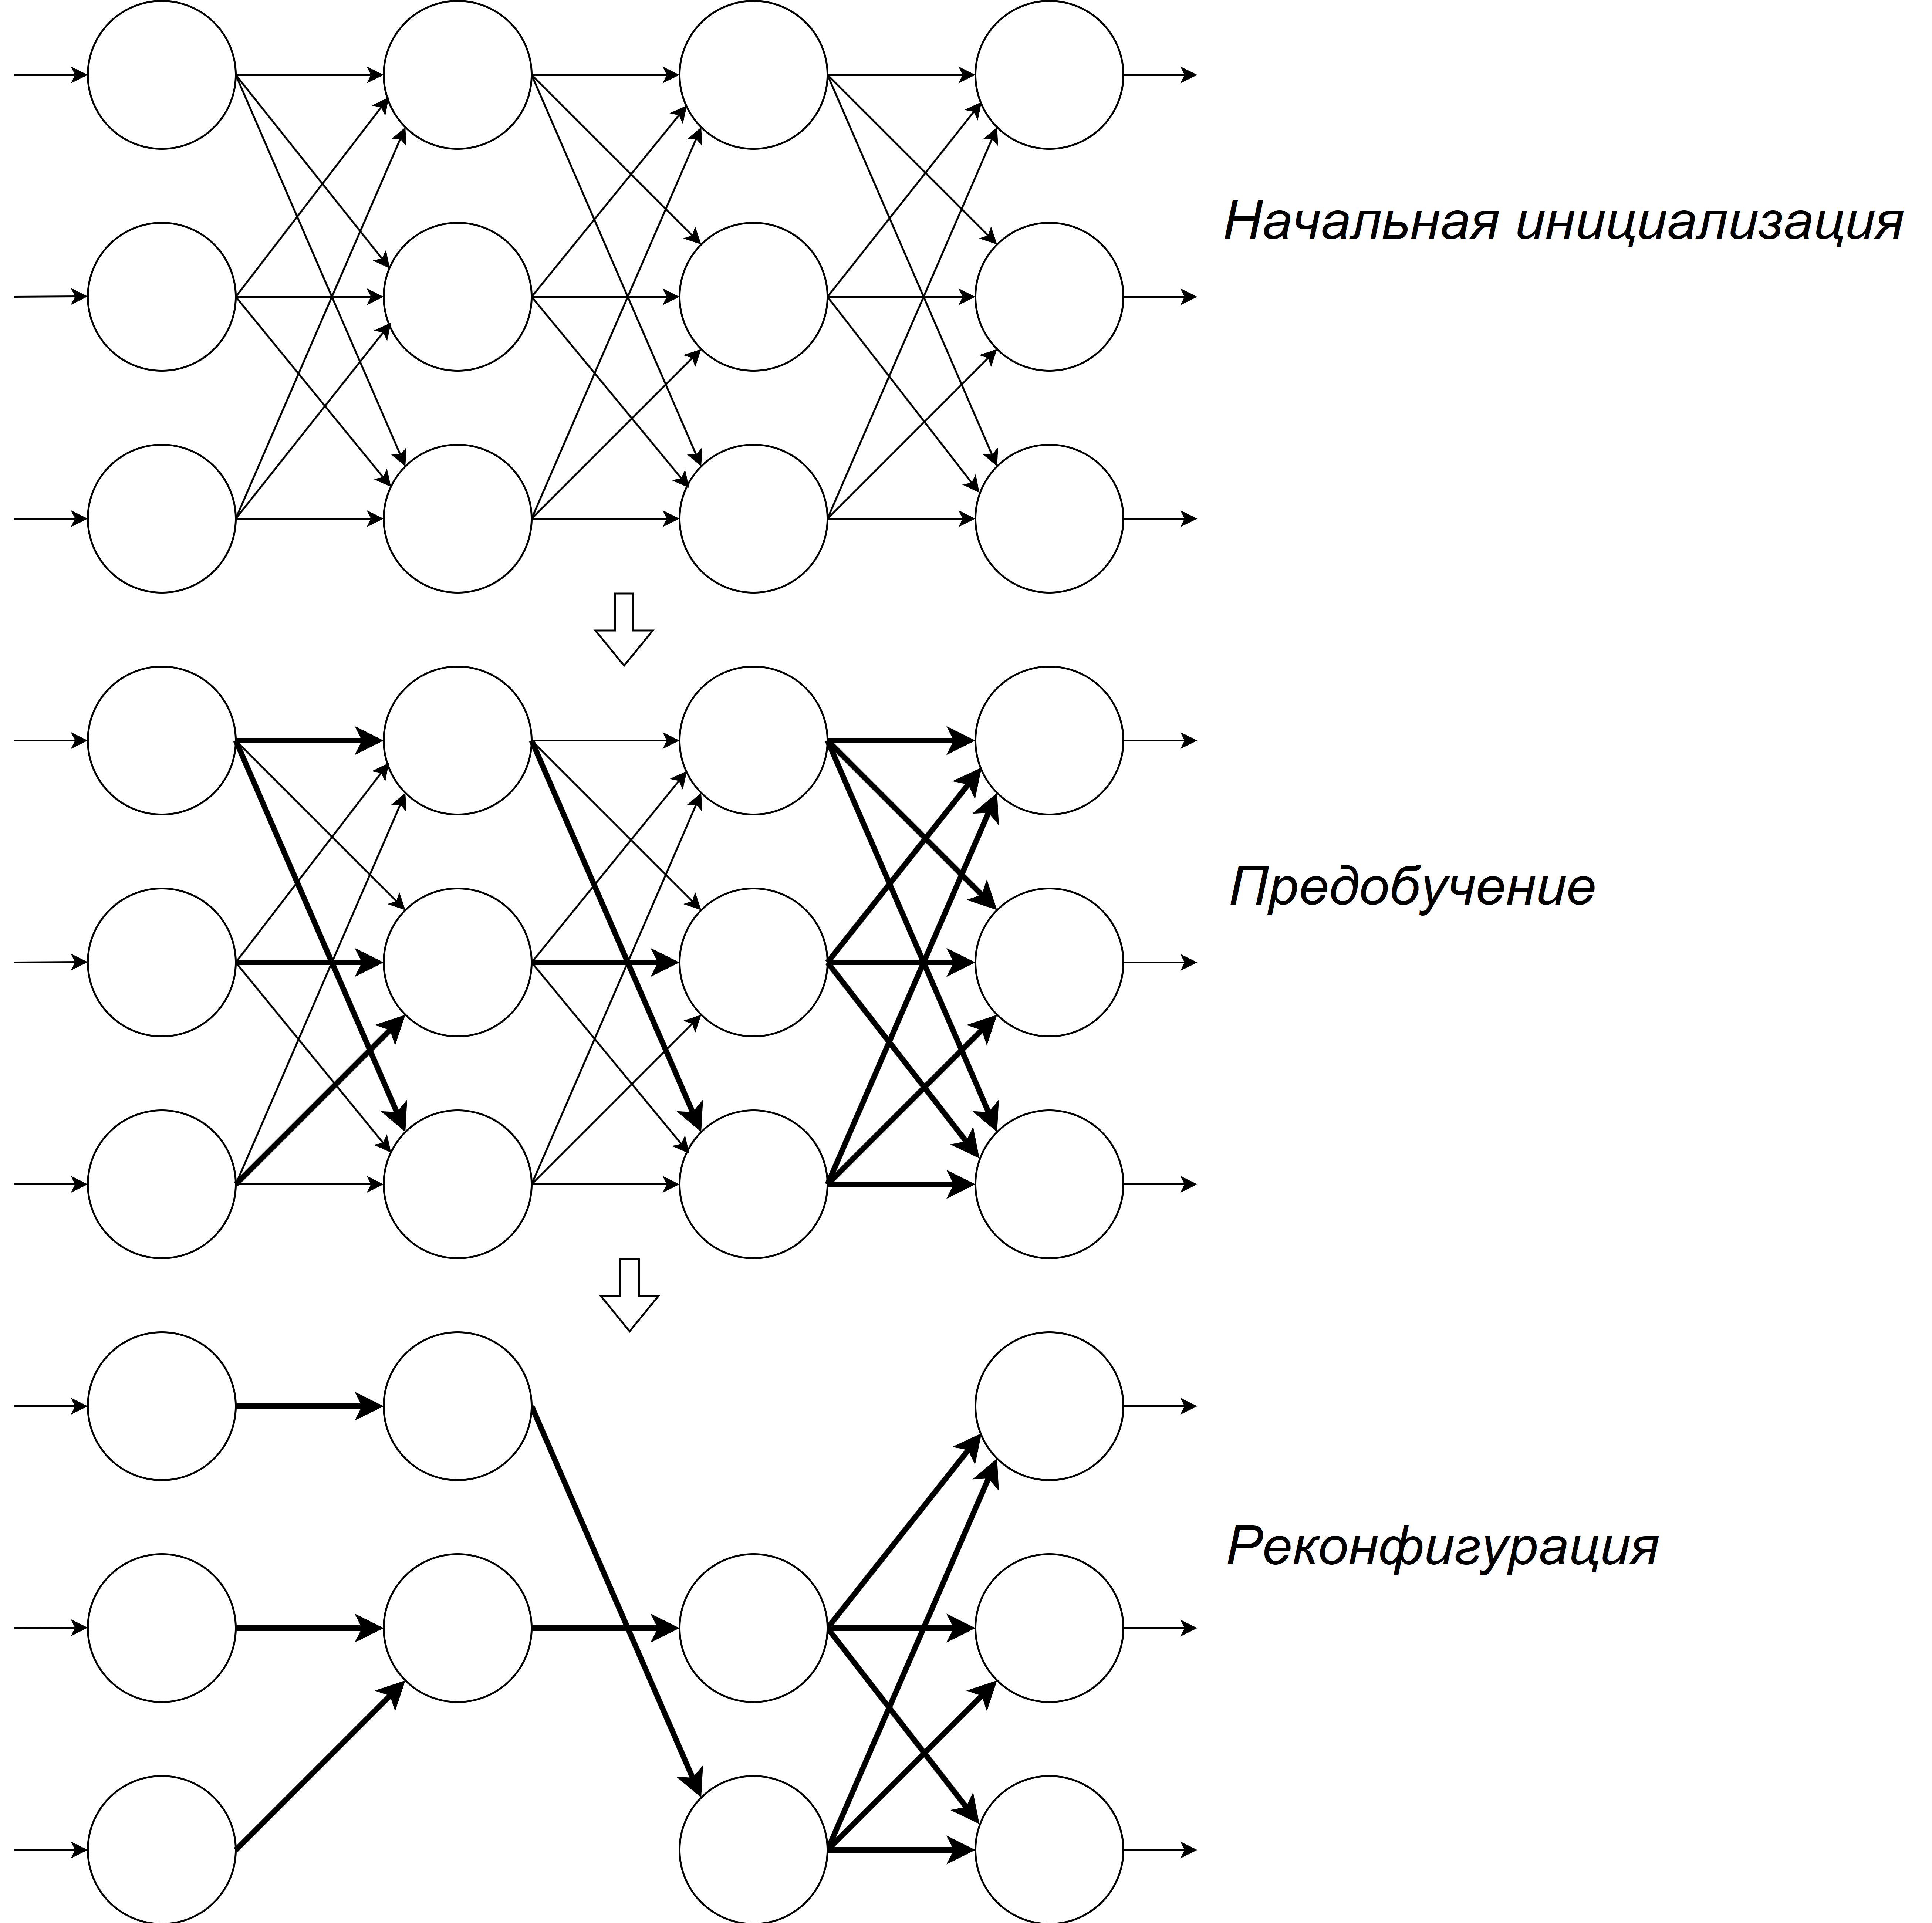
\includegraphics[width=0.7\textwidth]{man-source/images/ch2/pic2-3-1.png}
  \caption{Выполнение редуцирования весовых коэффициентов\\ с архитектурной реконфигурацией НС}
  \label{fig:pic2_3}
\end{figure}

% Этап 3 метода редуцирования может быть представлен следующим алгоритмом:

% \begin{algo}[h]
% 	% \SetAlgoLined
	
% 	\KwIn{\textit{\textbf{x(0)}} -- вектор-образ из обучающей выборки,
% 		$\alpha$ - скорость обучения
% 	}
% 	\KwRes{матрица весовых коэффициентов \textit{\textbf{W}}, вектор порогов нейронов видимого слоя $\textit{\textbf{V}}$, вектор порогов нейронов скрытого слоя $\textit{\textbf{H}}$}
% 	\ForEach{нейрона скрытого слоя $j$}{
% 		Вычислить $P(y_{j}(0)=1|x_{i}(0))$ (для биномиальных нейронов sigmoid($\sum_{i}{w_{ij}x_{i}(0)}+H_j$))\;
% 		Генерировать $y_{j}(0) \in \{0, 1\}$ из $P(y_{j}(0)|x_i(0))$\;
% 	}
% 	\ForEach{нейрона видимого слоя $i$}
% 	{
% 		Вычислить $P(x_{i}(1)=1|y_j(0))$ (для биномиальных нейронов sigmoid($\sum_{j}{w_{ij}y_{j}(0)} + V_i$))\;
% 		Генерировать $x_{i}(1) \in \{0, 1\}$ из $P(x_{i}(1)|y_j(0))$\;
% 	}	
% 	\ForEach{скрытых нейронов $j$}
% 	{
% 		Вычислить $P(y_{j}(1)=1|x_i(1))$ (для биномиальных нейронов sigmoid($\sum_{i}{w_{ij}x_{i}(1)} + H_j$))\;
% 	}
% 	$\textit{\textbf{W}} \leftarrow \textit{\textbf{W}} + \alpha(\textbf{\textit{x(0)}}\textit{\textbf{y(0)}}^T - \textit{\textbf{x(1)}}P(\textit{\textbf{y(1)}}=1|\textit{\textbf{x(1)}})^T)$\;
% 	$\textit{\textbf{V}} \leftarrow \textit{\textbf{V}} + \alpha(\textit{\textbf{x(0)}} - \textit{\textbf{x(1)}})$\;
% 	$\textit{\textbf{H}} \leftarrow \textit{\textbf{H}} + \alpha(\textit{\textbf{y(0)}} - P(\textit{\textbf{y(1)}}=1|\textit{\textbf{x(1)}}))$\;
% %	\While{not at end of this document}{
% %		read current\;
% %		\eIf{understand}{
% %			go to next section\;
% %			current section becomes this one\;
% %		}{
% %		go back to the beginning of current section\;
% %	}
% %}
%     \caption{Процедура обучения RBM}
% 	\label{rbm_learning}
% \end{algo}

% \begin{figure}
% 	\begin{center}
% 		\includegraphics[width=120mm]{reducing_weights.png}
% 		\caption{Метод редуцирования весовых коэффициентов}				
% 		\label{reducing_weigths}
% 	\end{center}
% \end{figure}

% Согласно полученным экспериментальным данным, приведенным в главе \ref{chapt3}, выбор заданного порогового параметра на шаге 2 позволяет значительно упростить архитектуру нейронной сети, сократив количество параметров до 80\% относительно их исходного количества без существенных потерей в обобщающей способности нейронной сети. Данный метод наглядно демонстрирует высокую степень избыточности полносвязных архитектур, используемых для решения задач с небольшими обучающими выборками.

\section{Выводы}
\begin{easylistNum}
    & Предложен альтернативный подход к обучению ограниченной машины Больцмана, базирующийся на идее минимизации суммарной квадратичной ошибки восстановления образов на скрытом и видимом слоях. 
    & Доказана теорема об эквивалентности максимизации функции правдоподобия распределения входных данных \textit{P(x)} и минимизации суммарной квадратичной ошибки восстановления образов на скрытых и видимых слоях в одном и том же пространстве синаптических связей ограниченной машины Больцмана при использовании линейных нейронов.
    & Доказана теорема об эквивалентности максимизации функции правдоподобия распределения входных данных \textit{P(x)} минимизации кросс-энтропийной целевой функции $CE_s(k)$ в одном и том же пространстве синаптических весов ограниченной машины Больцмана (случаи CD-1 и CD-k).
    & Сформулирована обобщающая теорема об эквивалентности максимизации функции правдоподобия распределения входных данных P(x), минимизации кросс-энтропийной функции, минимизации суммарной квадратичной ошибки (специальный случай) в одном и том же пространстве синаптических весов ограниченной машины Больцмана.
    & Приведены правила обучения для различных случаев линейной и нелинейной машины Больцмана (RBM).
    % & Приведены правила обучения для нелинейной ограниченной машины Больцмана (случаи CD-1 и CD-k).
    % & Приведены правила группового обучения для линейной ограниченной машины Больцмана (случаи CD-1 и CD-k).
    % & Приведены правила группового обучения для нелинейной ограниченной машины Больцмана (случаи CD-1 и CD-k).
    & Приведены правила для обучения сверточных слоев ГНС с использованием модели CRBM.
    & Предложен метод редуцирования параметров глубокой полносвязной нейронной сети, основывающийся на использовании процедуры неконтролируемого предобучения слоев.
\end{easylistNum}
% \chapter{УНИФИЦИРОВАННЫЕ СЕМАНТИЧЕСКИЕ МОДЕЛИ ОБРАБОТКИ ЗНАНИЙ}

% %\addcontentsline{toc}{chapter}{\introname}	% Добавляем его в оглавление

% Общий принцип организации обработки информации, хранимой в семантической памяти ostis-системы, может быть иллюстрирован следующим образом (рисунок \ref{fig:pic_kpp}):
% \begin{figure}[H]
%   \centering
%   \includegraphics[width=\textwidth]{man-source/images/ch2/pic_kpp.jpg}
%   \caption{Организация обработки информации в ostis-системе}
%   \label{fig:pic_kpp}
% \end{figure}

% В соответствии с приведенной иллюстрацией объединенный решатель задач разделяется на платформенно зависимую часть (scp-интерпретатор) и платформенно независимую часть -- программу объединенного решателя. Программа решателя хранится в той же памяти, что и обрабатываемые знания, в той же памяти взаимодействуют и информационные процессы, выполняемые агентами решателя и направленные на решение каких либо задач. В рамках программы решателя выделяется модель операционной семантики языка SCP, т. е. модель scp-интерпретатора, которая реализуется в рамках платформы. В свою очередь, абстрактная sc-память реализуется в виде sc-хранилища. 

% Таким образом, в рамках данной главы основное внимание будет уделено:
% \begin{easylist}
% &	модели взаимодействия информационных процессов, выполняемых в семантической памяти, включающей классификацию таких процессов, механизмы регулирования их выполнения, средства решения различных конфликтов, в том числе связанных с параллельным выполнением таких процессов, средства спецификации состояния информационных процессов (выполняемый, отложенный, планирумеый и т. д.);
% &	агентно-ориентированной модели гибридного решателя задач, который является субъектом, выполняющим указанные информационные процессы и, соответственно, модель которого строится с учетом указанной модели взаимодействия информационных процессов.
% \end{easylist}

% Указанные модели тесно связаны между собой, в связи с чем задачи по их разработке разделяются на схожие подзадачи (рисунок~\ref{fig:pic2_1}).

% \begin{figure}[H]
%   \centering
%   \includegraphics[width=\textwidth]{man-source/images/ch2/pic2_1.pdf}
%   \caption{Структура главы 2}
%   \label{fig:pic2_1}
% \end{figure}

% В рамках технологии OSTIS основным средством спецификации предметных областей являются \textit{онтологии}. Представленная на рисунке \ref{fig:pic2_1} задачно-ориентированная спецификация определяет структуру данной главы диссертационного исследования, в рамках которой последовательно описываются:
% \begin{easylist}
% &	онтология действий и задач, уточняющая формальные средства спецификации преобразований, выполняемых различными субъектами в памяти компьютерной системы и за ее пределами;
% &	онтология действий в sc-памяти, уточняющая виды действий, выполняемых в такой памяти (информационных процессов);
% &	онтология sc-агентов, являющихся субъектами, выполняющими информационные процессы в sc-памяти;
% &	средства синхронизации выполнения параллельных информационных процессов в семантической памяти;
% &	онтология scp-программ, уточняющая понятие прогрраммы языка SCP, классификацию операторов языка SCP, средства их спецификации;
% &	агентно-ориентированная модель гибридного решателя задач, построенная на основе всех перечисленных онтологий;
% &	онтология интерпретатора scp-программ, который рассматривается как своего рода решатель задач частного вида и, соответственно, строится с использованием указанной выше модели. Данная онтология уточняет перечень агентов интерпретатора и их спецификацию.

% \end{easylist}

% Далее рассмотрим более подробно каждый из компонентов предложенной модели.
% \newpage
% \section[Формальная модель взаимодействия информационных процессов в семантической памяти]{Формальная модель взаимодействия информационных процессов\\ в семантической памяти}

% Формально модель взаимодействия информационных процессов в семантической памяти задается следующим образом:

% \begin{equation} 
% \label{<eq2_1>} 
% M_{IPM} = \{M_A, M_S, M_{SYNC}, M_{SCP}\},
% \end{equation} 

% \parindent=8mm
% \noindent \hangindent=22mm \hangafter=1
% где $M_A$ – модель деятельности, выполняемой различными субъектами (агентами) в памяти компьютерной системы и за ее пределами;

% \hangindent=22mm \hangafter=1
% $M_S$ – модель субъекта (агента), осуществляющего преобразования в семантической памяти компьютерной системы;

% \hangindent=30mm \hangafter=1
% $M_{SYNC}$ – модель синхронизации выполнения процессов в семантической памяти компьютерной системы;

% \hangindent=27mm \hangafter=1
% $M_{SCP}$ – модель базового языка программирования, ориентированного на обработку унифицированных семантических сетей, которая, в свою очередь, задается как

% \begin{equation} 
% \label{<eq2_2>} 
% M_{SCP} =\{M_P, M_I\},	
% \end{equation} 

% \noindent \hangindent=22mm \hangafter=1
% где $M_P$ – модель программы базового языка программирования;

% \hangindent=22mm \hangafter=1
% $M_I$ – модель интерпретатора программ базового языка программирования.

% \parindent=10mm

% Графическая иллюстрация модели взаимодействия процессов может быть приведена на рисунке \ref{fig:pic_proc_model}.

% \begin{figure}[H]
%   \centering
%   \includegraphics[width=0.7\textwidth]{man-source/images/ch2/pic_proc_model.pdf}
%   \caption{Модель взаимодействия процессов в семантической памяти}
%   \label{fig:pic_proc_model}
% \end{figure}

% Как видно из рисунка, в соответствии с изложенными ранее принципами агенты не обмениваются сообщениями напрямую, коммуникация между агентами осуществляется посредством спецификации выполняемых ими информационных процессов. В свою очередь, синхронизация выполнения параллельных информационных процессов осуществляется с использованием механизма блокировок элементов семантической памяти. Спецификация каждого информационного процесса фиксируется в семантической памяти. Каждый агент также имеет соответствующую спецификацию, которая является частью базы знаний системы и содержит сведения об условиях инициирования данного агента, возможных результатах его работы, ключевых элементах и т. д.

% Далее рассмотрим более подробно компоненты предложенной модели.

% \newpage
% \section{Формальные средства описания деятельности различных субъектов в семантической памяти} \label{section_actions}

% Модель деятельности, выполняемой различными субъектами (агентами) в памяти компьютерной системы и за ее пределами, задается следующим образом:

% \begin{equation} 
% \label{<eq2_3>} 
% M_A = \{A_C, A_{CM}, A_R, A_{CS}\},	
% \end{equation} 

% \parindent=8mm
% \noindent \hangindent=22mm \hangafter=1
% где $A_C$ – множество классов действий, выполняемых различными субъектами;

% \hangindent=25mm \hangafter=1
% $A_{CM}$ – множество классов действий, выполняемых агентами в семантической памяти, $A_{CM} \subset A_C$;

% \hangindent=22mm \hangafter=1
% $A_R$ – набор отношений, специфицирующих действия, принадлежащие классам из $A_C$;

% \hangindent=22mm \hangafter=1
% $A_{CS}$ – множество классов спецификаций действий, принадлежащих классам из $A_C$, таких как задача, протокол выполнения некоторого действия и т. д.;

% \parindent=10mm

% Более детально каждый компонент модели специфицируется в рамках \textit{предметной области действий и задач}. В рамках указанной предметной области исследуются такие общие понятия, как действие, субъект, объект действия, задача и ее решение и т. д. 

% Семантическая теория деятельности подробно рассматривается в работах В. В. Мартынова \cite{Martynov1974,Martynov1977,Martynov1984}, а также его учеников, в частности, в работе \cite{Boyko2016}. В указанных работах подробно рассматривается семантическая классификация действий, описываются подходы к формализации описания деятельности различного рода субъектов с использованием разработанного В. В. Мартыновым Универсального семантического кода (УСК). В этих работах детально рассматриваются такие понятия, как воздействие, субъект воздействия (агент), объект и другие, рассматриваемые также и в данной работе. 

% Кроме того, в работе \cite{Schenk1980} рассматриваются такие понятия, близкие рассматриваемым в данной работе, как воздействие, действие (акт), деятель (субъект) и другие.

% Задачей данной диссертационной работы, в отличие от указанных, является разработка средств описания деятельности различных субъектов в памяти компьютерной системы на основе SC-кода. Разработка таких средств позволит реализовать и интегрировать на их основе результаты, полученные в указанных работах, и использовать их в дальнейшем, в том числе при разработке различных решателей задач.

% \subsection{Общее понятие действия}

% В рамках предлагаемой модели описания деятельности понятие \textit{действие} является частным случаем понятия \textit{воздействие}, которое рассматривается в более общих предметных областях в рамках базы знаний IMS \cite{IMS2017}.
% В свою очередь, воздействие является частным случаем \textit{процесса}. Каждый \textit{процесс} определяется (задается) либо возникновением или исчезновением связей, связывающих заданную \textit{временную сущность} с другими сущностями, либо части указанной \textit{временной сущности} с другими сущностями. С точки зрения классификации фрагментов базы знаний \cite{Davydenko2016a} \textit{процесс} представляет собой ситуативную структуру, в каждый момент времени описывающую текущее состояние объектов, участвующих в данном процессе. \textit{Процесс}, описывающий изменения, происходящие исключительно в рамках sс-памяти, будем называть \textit{процессом в sc-памяти}.
% Каждому \textit{воздействию} может быть поставлена в соответствие 
% \begin{easylist}
% & некоторая \textit{воздействующая сущность* (субъект)}, т. е. сущность, осуществляющая воздействие (в частности, это может быть некоторое физическое поле);
% & некоторый \textit{объект воздействия*}, т. е. сущность, на которую воздействие направлено.
% \end{easylist}
% Если \textit{воздействие} связано с \textit{материальной сущностью}, то его объектом воздействия является либо сама эта \textit{материальная сущность}, либо некоторая ее пространственная часть.
% В свою очередь, каждое \textit{действие}, выполняемое тем или иным \textit{субъектом}, одновременно можно трактовать и как процесс решения некоторой задачи, т. е. как процесс достижения заданной цели в заданных условиях.
% Предполагается, что любое \textit{действие}, выполняемое каким-либо \textit{субъектом}, направлено на решение какой-либо задачи и выполняется \underline{целенаправленно}. При этом явное указание \textit{действия} и его связи с конкретной \textit{задачей} может не всегда присутствовать в памяти. Некоторые задачи могут решаться определенными агентами перманентно, например, оптимизация базы знаний, поиск некорректностей и т. д., и для подобных задач не всегда есть необходимость явно вводить \textit{структуру} \cite{Davydenko2016a}, являющуюся формулировкой \textit{задачи}.
% Каждое \textit{действие} обозначает некоторое преобразование, осуществляемое во внешней среде либо в памяти некоторой системы, однако в памяти явно вводятся только sc-элементы, обозначающие те \textit{действия}, для которых есть необходимость явно хранить их спецификацию в течение некоторого времени.
% При выполнении действия можно выделить следующие этапы:
% \begin{easylist}
% &	построение плана деятельности, декомпозиция исходного действия;
% &	выполнение построенного плана действий;
% \end{easylist}
% Формальная спецификация понятия действие в SCn-коде (в том числе – классификация действий с пояснениями) приведена в приложении \ref{AppendixActions}.

% В процессе описания в семантической памяти деятельности некоторого коллектива субъектов возникает необходимость выделять в рамках этой деятельности обособленные логически целостные фрагменты, которые могут выполняться отдельными субъектами независимо друг от друга.

% Спецификация понятия \textit{класса действий} в SCn-коде:

% \begin{flushleft}

% \noindent\setlength{\hangindent}{1em} 
% \hspace{-0.3em}\textbf{\itshape класс действий}\\
% $=${\itshape множество действий, однотипных в том или ином смысле}\\
% $<=$ {\itshape семейство подмножеств*}:\\
% \hspace{2em}{\itshape действие}\\
% $<=$ {\itshape разбиение*}:\\
% \hspace{2em}$\{$\\
% \hspace{3em}{$\bullet$ \itshape класс логически атомарных действий} \\
% \hspace{4em}$=${\itshape класс автономных действий}\\
% \hspace{3em}{$\bullet$ \itshape класс логически неатомарных действий} \\
% \hspace{4em}$=${\itshape класс неавтономных действий}\\
% \hspace{2em}$\}$
% \end{flushleft}

% Каждое \textit{действие}, принадлежащее некоторому конкретному \textit{классу логически атомарных действий}, обладает двумя необходимыми свойствами:
% \begin{easylist}
% & выполнение действия не зависит от того, является ли указанное действие частью декомпозиции более общего действия. При выполнении данного действия также не должен учитываться тот факт, что данное действие предшествует каким-либо другим действиям или следует за ними (что явно указывается при помощи отношения \textit{последовательность действий*});
% & указанное действие должно представлять собой логически целостный акт преобразования, например, в семантической памяти. Такое действие по сути является транзакцией, т. е. результатом такого преобразования становится новое состояние преобразуемой системы, а выполняемое действие должно быть либо выполнено полностью, либо не выполнено совсем, частичное выполнение не допускается. 
% \end{easylist}

% В то же время логическая атомарность не запрещает декомпозировать выполняемое действие на более частные, каждое из которых, в свою очередь, также будет являться логически атомарным. На рисунке \ref{fig:pic_laa} с использованием языка SCg показан пример декомпозиции более сложного логически атомарного действия на более простые.

% \begin{figure}[H]
%   \centering
%   \includegraphics[width=0.8\textwidth]{man-source/images/ch2/pic_laa.png}
%   \caption{Декомпозиция логически атомарного действия на поддействия}
%   \label{fig:pic_laa}
% \end{figure}

% На логически атомарные действия предлагается делить всю деятельность, направленную на решение каких-либо задач ostis-системой. Соответственно решатель предлагается делить на компоненты (агенты), соответствующие таким классам логически атомарных действий, что является основой для обеспечения его \textbf{модифицируемости}.

% В случае действий, выполняемых в семантической памяти, степень детализации каждого такого действия ограничивается синтаксическими особенностями используемого варианта представления знаний. В случае SC-кода можно выделить такие классы элементарных действий, как создание sc-элемента заданного типа, удаление sc-элемента, поиск sc-элементов, инцидентных указанному sc-элементу. На основе классификации таких элементарных преобразований в семантической памяти строится язык SCP, который описывается ниже в разделе~\ref{section_scp}.

% Предполагается, что каждое действие выполняется целенаправленно некоторым \textit{субъектом}. Формальная спецификация понятия \textit{субъект} в \mbox{SCn-коде} (в том числе – классификация субъектов):

% \begin{flushleft}

% \noindent\setlength{\hangindent}{1em} 
% \hspace{-0.3em}\textbf{\itshape субъект}\\
% $=${\itshape активная сущность}\\
% $=${\itshape сущность, способная самостоятельно выполнять некоторые виды действий}\\
% $=>$ {\itshape включение*}:\\
% \hspace{2em}{$\bullet$ \itshape собственное я ostis-системы} \\
% \hspace{2em}{$\bullet$ \itshape внутренний субъект ostis-системы} \\
% \setlength{\hangindent}{3em}
% \hspace{2em}{$\bullet$ \itshape внешний субъект ostis-системы, с которым осуществляется взаимодействие} \\
% \hspace{2em}{$\bullet$ \itshape внешний субъект ostis-системы, с которым взаимодействие не происходит} \\
% \end{flushleft}

% Под \textit{внутренним субъектом ostis-системы} понимается такой \textit{субъект}, который выполняет некоторые \textit{действия} в \underline{той же памяти}, в которой хранится его знак.

% К числу \textit{внутренних субъектов ostis-системы} относятся входящие в нее \textit{агенты}, отдельные решатели задач, целые интеллектуальные подсистемы.

% К числу \textit{внешних субъектов ostis-системы, с которыми осуществляется взаимодействие}, относятся конечные пользователи \textit{ostis-системы}, ее разработчики, а также другие компьютерные системы (причем, не только интеллектуальные).

% \subsection[Средства детализации процесса выполнения\\ действий]{Средства детализации процесса выполнения действий}

% Рассмотрим набор отношений, предназначенных для описания детализации процесса выполнения того или иного действия, т. е. выделения более простых частных действий.

% Связки отношения \textit{декомпозиция действия*} связывают \textit{действие} и множество частных \textit{действий}, на которые декомпозируется данное действие. При этом первым компонентом связки является знак указанного множества, вторым компонентом – знак более общего \textit{действия}.

% Таким образом, \textit{декомпозиция действия*} это \textit{квазибинарное отношение} \cite{IMS2017}, связывающее действие со множеством действий более низкого уровня, к выполнению которых сводится выполнение исходного декомпозируемого действия.

% Стоит отметить, что каждое \textit{действие} может иметь несколько вариантов декомпозиции в зависимости от конкретного набора элементарных действий, которые способна выполнять та или иная система \textit{субъектов}.

% Принцип, по которому осуществляется такая декомпозиция в различных подходах к решению задач, будем называть \underline{стратегией решения задач}.

% Кроме того, для детализации процесса выполнения действий используется отношение \textit{поддействие*}, связки которого связывают \textit{действие} и некоторое более простое частное \textit{действие}, выполнение которого необходимо для выполнения исходного более общего \textit{действия}.

% Для описания порядка выполнения действий используется отношение \textit{последовательность действий*}, частными видами которого являются отношения \textit{последовательность действий при положительном результате*} и \textit{последовательность действий при отрицательном результате*}.

% Связки отношения \textit{последовательность действий*} связывают знаки \textit{действий}, выполняющихся в какой-либо последовательности в процессе решения какой-либо задачи. При этом считается, что если два \textit{действия} связаны данным отношением, то \textit{действие}, стоящее в данной связке на втором месте, может быть выполнено только после выполнения действия, стоящего в данной связке на первом месте. Таким образом, каждое действие может быть инициировано после завершения выполнения любого из предшествующих действий.

% Переход по связкам отношения \textit{последовательность действий при положительном результате*} от предшествующего действия проверки условия к последующему действию происходит при условии, если указанная проверка даст положительный результат, т. е. предшествующее действие станет \textit{успешно выполненным действием}.

% Переход по связкам отношения \textit{последовательность действий при отрицательном результате*} от предшествующего действия проверки условия к последующему действию происходит при условии, если указанная проверка даст отрицательный результат, т. е. предшествующее действие станет \textit{безуспешно выполненным действием}.

% Для обеспечения возможности синхронизации выполнения действий используется класс действий \textit{конъюнкция предшествующих действий}. Действия указанного класса используются в тех случаях, когда выполнение некоторого действия должно начаться только после того, как будут выполнены все предшествующие действия, а не только одно из них. После того как все предшествующие действия выполнены, инициируются действия, следующие за \textit{конъюнкцией предшествующих действий}.

% В некоторых случаях бывает необходимо управлять процессом выполнения какой-либо последовательности действий в зависимости от выполнения дополнительных условий. Для осуществления таких проверок вводится класс действий \textit{проверки условия}. Действия класса \textit{проверка условия} предполагают проверку истинности или ложности некоторого высказывания (условия), и после выполнения в зависимости от результата данной проверки становятся \textit{успешно выполненными действиями} или \textit{безуспешно выполненными действиями}.

% Следует отметить, что предлагаемый подход к описанию переходов между действиями очень близок к решениям, описанным в уже упоминавшейся статье \cite{Kotov1966}. Действительно, каждое действие независимо от его сложности можно считать аналогом процессорного элемента, рассмотренного в указанной статье, а условием инициирования какого-либо действия (спусковой функцией) является факт завершенности хотя бы одного из предыдущих действий (т. е. связанных с текущим действием связкой отношения \textit{последовательность действий*} или более частных отношений). Таким образом, использование предлагаемого языка описания деятельности различных субъектов на различных уровнях позволит не только говорить об универсальности и «понятности» такого описания за счет использования самых базовых понятий, но и о возможности реализации различных моделей \underline{параллелизма на любом уровне}, начиная от параллельного выполнения операторов в рамках одной программы, заканчивая взаимодействием целых коллективов агентов в общей семантической памяти. Возможность реализации той или иной модели параллелизма в таком случае определяется исключительно особенностями решаемой задачи.


% \subsection{Спецификация действий}
% Важнейшим с точки зрения функционирования системы понятием является понятие задачи. Под \textit{задачей} понимается формальная спецификация некоторого действия (условие), достаточная для выполнения данного действия каким-либо \textit{субъектом}. В зависимости от конкретного класса задач описываться может как внутреннее состояние самой интеллектуальной системы, так и требуемое состояние внешней среды. \textit{sc-элемент}, обозначающий \textit{действие}, входит в \textit{задачу} под атрибутом \textit{ключевой sc-элемент'}.

% Классификация задач может осуществляться по дидактическому признаку в рамках каждой предметной области, например, задачи на треугольники, задачи на системы уравнений и т. п.

% Каждая \textit{задача} может включать:
% \begin{easylist}
% &	факт принадлежности \textit{действия} какому-либо частному классу \textit{действий} (например, \textit{действие. сформировать полную семантическую окрестность указываемой сущности}), в том числе состояние \textit{действия} с точки зрения жизненного цикла (инициированное, выполняемое и т. д.);
% &	описание \textit{цели* (результата*) действия}, если она точно известна;
% &	указание \textit{заказчика* действия};
% &	указание \textit{исполнителя* действия} (в том числе коллективного);
% &	указание \textit{аргумента(ов) действия’};
% &	указание инструмента или посредника \textit{действия};
% &	описание \textit{декомпозиции действия*};
% &	указание \textit{последовательности действий*} в рамках \textit{декомпозиции действия*}, т.е построение плана решения задачи. Другими словами, построение плана решения представляет собой декомпозицию соответствующего \textit{действия} на систему взаимосвязанных между собой поддействий;
% &	указание области \textit{действия};
% &	указание условия инициирования действия;
% &	момент начала и завершения \textit{действия}, в том числе планируемый и фактический, предполагаемая и/или фактическая длительность выполнения.

% \end{easylist}

% Некоторые задачи могут быть дополнительно уточнены контекстом – дополнительной информацией о сущностях, рассматриваемых в формулировке \textit{задачи}, т. е. описанием того, что дано, что известно об указанных сущностях.

% Кроме этого, \textit{задача} может включать любую дополнительную информацию о действии, например:
% \begin{easylist}
% &	перечень ресурсов и средств, которые предполагается использовать при решении задачи, например, список доступных исполнителей, временные сроки, объем имеющихся финансов и т. д.;
% &	ограничение области, в которой выполняется действие, например, необходимо заменить одну sc-конструкцию на другую по некоторому правилу, но только в пределах некоторого раздела базы знаний;
% &	ограничение знаний, которые можно использовать для решения той или иной задачи, например, необходимо решить задачу по алгебре, используя только те утверждения, которые входят в курс школьной программы до седьмого класса включительно, и не используя утверждения, изучаемые в старших классах;
% &	и прочее.
% \end{easylist}
% С одной стороны, решаемые системой задачи можно классифицировать на \textit{информационные задачи} и \textit{поведенческие задачи}. 

% С точки зрения формулировки поставленной задачи можно выделить \textit{декларативные формулировки задачи} и \textit{процедурные формулировки задачи}. Следует отметить, что данные классы задач не противопоставляются, и могут существовать формулировки задач, использующие оба подхода.

% В случае \textit{процедурной формулировки задачи} в формулировке задачи явно указываются аргументы соответствующего задаче \textit{действия} и, в частности, вводится семантическая классификация \textit{действий}. При этом явно не уточняется, что должно быть результатом выполнения данного действия. Заметим, что при необходимости \textit{процедурная формулировка задачи} может быть сведена к \textit{декларативной формулировке задачи} путем трансляции на основе некоторого правила, например, определения класса действия через более общий класс.

% В случае \textit{декларативной формулировки задачи} при описании условия задачи специфицируется цель \textit{действия}, т. е. результат, который должен быть получен при успешном выполнении \textit{действия}.

% В свою очередь, под \textit{вопросом} понимается задача, направленная на удовлетворение информационной потребности некоторого субъекта-заказчика.

% Под \textit{командой} (в том числе – \textit{интерфейсной командой}) понимается спецификация инициированного действия (инициированная задача).

% Рассмотрим набор отношений, используемых для формальной спецификации действий в рамках \textit{задачи}.

% Связки отношения \textit{результат*} связывают \textit{sc-элемент}, обозначающий \textit{действие}, и \textit{sc-конструкцию}, описывающую результат выполнения рассматриваемого действия, другими словами, цель, которая должна быть достигнута при выполнении \textit{действия}.

% Результат может специфицироваться как атомарным высказыванием, так и неатомарным, т. е. конъюнктивным, дизъюнктивным, строго дизъюнктивным и т. д.
% В случае, когда успешное выполнение \textit{действия} приводит к изменению какой-либо конструкции в \textit{sc-памяти}, которое необходимо занести в историю изменений базы знаний или использовать для демонстрации протокола решения задачи, генерируется соответствующая связка отношения \textit{результат*}, связывающая \textit{задачу} и \textit{sc-конструкцию}, описывающую данное изменение. Конкретный вид указанной \textit{sc-конструкции} зависит от типа действия.

% Связки отношения \textit{исполнитель*} связывают \textit{sc-элементы}, обозначающие \textit{действие} и \textit{sc-элементы}, обозначающие \textit{субъекта}, который предположительно будет осуществлять, осуществляет или осуществлял выполнение указанного \textit{действия}. Данное отношение может быть использовано при назначении конкретного исполнителя для проектной задачи по развитию баз знаний.

% В случае, когда заранее неизвестно, какой именно \textit{субъект*} будет исполнителем данного \textit{действия}, связка отношения \textit{исполнитель*} может отсутствовать в первоначальной формулировке \textit{задачи} и добавляться позже, уже непосредственно при исполнении.

% Когда действие выполняется (является \textit{настоящей сущностью}) или уже выполнено (является \textit{прошлой сущностью}), то исполнитель этого действия в каждый момент времени уже определен.

% Связки отношения \textit{заказчик*} связывают \textit{sc-элементы}, обозначающие \textit{действие}, и \textit{sc-элементы}, обозначающие \textit{субъекта}, который <<заинтересован>> в выполнении данного действия и, как правило, инициирует его выполнение. Данное отношение может быть использовано при указании того, кто поставил проектную задачу по развитию базы знаний.

% Связки отношения \textit{объект*} связывают \textit{sc-элемент}, обозначающий \textit{действие}, и знак той сущности, над которой (по отношению к которой) осуществляется данное \textit{действие}, например, знак \textit{структуры}, подлежащий верификации.

% Связки отношения \textit{контекст действия*} связывают \textit{sc-элементы}, обозначающие \textit{действие} и \textit{структуры}, обозначающие контекст выполнения данного \textit{действия}, т. е. некоторую дополнительную информации о тех сущностях, которые входят в описание \textit{цели*}. Как правило, контекст используется для указания собственно условия некоторой задачи, того, что дано, т. е. тех знаний, которые можно использовать для вывода новых знаний при решении задачи. Таким образом, контекст непосредственно влияет на то, как будет решаться та или иная задача, при этом даже задачи, соответствующие одному классу действий, могут решаться по-разному.

% Контекст может быть представлен не только в виде атомарного фактографического высказывания, но и в виде высказывания более сложного вида. Это может быть, например:
% \begin{easylist}
% &	определение множества, используемого в описании \textit{цели*};
% &	утверждение, учет которого может быть полезен в решении задач.
% \end{easylist}
% В случае процедурной формулировки задачи для указания в рамках конкретного действия тех sc-элементов, над которыми непосредственно выполняется данное действие, используется ролевое отношение \textit{аргумент действия'}.

% Для уточнения класса сущностей, которые могут быть аргументами действий, соответствующих некоторому \textit{классу команд}, используется отношение \textit{класс аргументов*}. В случае, когда \textit{команды} данного класса имеют один аргумент, используется собственно отношение \textit{класс аргументов*}, в случае, когда больше команды данного класса имеют более одного аргумента, то используются подмножества данного отношения, такие, как \textit{класс первых аргументов*}, \textit{класс вторых аргументов*} и т. д.

% На рисунке \ref{fig:pic_probl_ex} с использованием языка SCg показан пример представления задачи в sc-памяти, связанной с установлением истинности высказывания о конгруэнтности двух треугольников.

% \begin{figure}[H]
%   \centering
%   \includegraphics[width=0.85\textwidth]{man-source/images/ch2/pic_probl_ex.png}
%   \caption{Пример представления задачи}
%   \label{fig:pic_probl_ex}
% \end{figure}

% Если для некоторого \textit{класса команд} не указан тип какого-либо из аргументов, то предполагается, что в качестве данного аргумента может выступать любой \textit{sc-элемент}.

% Кроме задачи как спецификации действия в целом необходимо выделить еще ряд \textit{семантических окрестностей} \cite{Davydenko2016a}, специфицирующих конкретное действие с той или иной стороны.

% \begin{easylist}
% &	План выполнения действия

% Каждый \textit{план} представляет собой \textit{семантическую окрестность}, ключевым \textit{sc-элементом'} является \textit{действие}, для которого дополнительно детализируется предполагаемый процесс его выполнения. Основная задача такой детализации – локализация области базы знаний, в которой предполагается работать, а также набора агентов, необходимого для выполнения описываемого действия. При этом детализация необязательно должна быть доведена до уровня элементарных действий, цель составления плана – уточнение подхода к решению той или иной задачи, не всегда предполагающее составления подробного пошагового решения.

% При описании \textit{плана} может быть использован как процедурный, так и декларативный подход. В случае процедурного подхода для соответствующего \textit{действия} указывается его декомпозиция на более частные поддействия, а также необходимая спецификация этих поддействий. В случае декларативного подхода указывается набор подцелей (например, при помощи логических утверждений), достижение которых необходимо для выполнения рассматриваемого \textit{действия}. На практике оба рассмотренных подхода можно комбинировать.

% В общем случае \textit{план} может содержать и переменные, например, в случае, когда часть плана задается в виде цикла (многократного повторения некоторого набора действий). Также план может содержать константы, значение которых в настоящий момент не установлено и станет известно, например, только после выполнения предшествующих ему \textit{действий}.

% Каждый \textit{план} может быть задан заранее как часть спецификации \textit{действия}, т. е. задачи, а может формироваться \textit{субъектом} уже собственно в процессе выполнения \textit{действия}, например, в случае использования стратегии разбиения задачи на подзадачи. В первом случае \textit{план включается*} в \textit{задачу}, соответствующую тому же действию.

% &	Программа выполнения класса действий

% Каждая \textit{программа} представляет собой обобщенный \textit{план} выполнения \textit{действий}, принадлежащих некоторому классу, т. е. \textit{семантическую окрестность}, \textit{ключевым sc-элементом'} является \textit{класс действий}, для элементов которого дополнительно детализируется процесс их выполнения.

% В остальном описание программы аналогично описанию \textit{плана} выполнения конкретного \textit{действия} из рассматриваемого \textit{класса действий}.

% Одному \textit{классу действий} может соответствовать несколько \textit{программ}.

% Входным параметрам \textit{программы} в традиционном понимании соответствуют аргументы, соответствующие каждому \textit{действию} из \textit{класса действий}, описываемого \textit{программой}. При генерации на основе \textit{программы плана} выполнения конкретного \textit{действия} из данного класса эти аргументы принимают конкретные значения.

% Каждая \textit{программа} представляет собой систему описанных действий с дополнительным указанием для действия:

% &	либо \textit{последовательности выполнения действий*} (передачи инициирования), когда условием выполнения (инициирования) действий является завершение выполнения одного из указанных или всех указанных действий;
% &	либо события в базе знаний или внешней среде, являющегося условием его инициирования;
% &	либо ситуации в базе знаний или внешней среде, являющейся условием его инициирования.
% \end{easylist}

% Видно, что предложенная трактовка понятия программы как обобщенного плана выполнения некоторого класса действий никак не ограничивает область его применения, в частности, как программа в таком смысле может трактоваться рецепт приготовления какого-либо блюда, обобщенное описание какого-либо технологического процесса, инструкция по использованию какого-либо устройства и т. д.

% Пример программы \textit{языка SCP} (scp-программы) представлен в приложении \ref{AppendixSCP} (рисунок \ref{img:examplescp1}). Более подробно сам \textit{язык SCP} будет рассмотрен ниже.

% Данный пример представляет собой \textit{scp-программу}, имеющую два аргумента (множество и элемент, который надо добавить во множество). В соответствии с алгоритмом программы осуществляется проверка того, имеется ли указанный элемент в указанном множестве, и если нет, то элемент добавляется во множество. В рамках данной программы исходный scp-процесс декомпозируется на три более простых подпроцесса (\textit{поддействия*}), связанных соответствующими подклассами отношения \textit{последовательность выполнения действий*}. Таким образом, программа состоит из трех элементарных действий (\textit{scp-операторов}) – поиск элемента во множестве, добавление элемента во множество и завершение выполнения, между которыми указаны два условных перехода и один безусловный. Часть используемых в данном примере понятий идентифицирована при помощи \textit{системных идентификаторов*} \cite{IMS2017}, например, \textit{nrel\_then, nrel\_else} и т. д.

% Кроме того, выделяются такие классы \textit{семантических окрестностей} действий, как \textit{протокол} выполнения действия, содержащий декомпозицию рассматриваемого \textit{действия} на поддействия с указанием порядка их выполнения, а также необходимой спецификацией каждого такого поддействия, и решение, в рамках которого указываются только те поддействия, без которых решение поставленной задачи было бы невозможным, т. е. из \textit{протокола} исключаются ложные или избыточные шаги, проделанные в процессе поиска пути решения задачи, которые, в свою очередь, могут присутствовать при описании непосредственно текущего хода решения задачи.

% \subsection{Классификация действий в семантической памяти} \label{section_actions_in_sc_memory}
% Отдельное внимание следует уделить действиям, выполняемым в семантической памяти компьютерной системы (sc-памяти).

% Описанные в данном подразделе понятия исследуются в рамках \textit{предметной области действий, выполняемых в абстрактной унифицированной семантической памяти} и представлены в соответствующем разделе базы знаний метасистемы IMS \cite{IMS2017}.

% Каждое \textit{действие в sc-памяти} обозначает некоторое преобразование, выполняемое некоторым \textit{субъектом} (или коллективом \textit{субъектов}) в рамках \mbox{\textit{sc-памяти}}. Спецификация действия после его выполнения может быть включена в протокол решения некоторой задачи. 

% Семантика каждого \textit{действия в sc-памяти} зависит от конкретного контекста, т. е. ориентации действия на какие-либо конкретные объекты и принадлежности действия какому-либо конкретному классу действий.

% Следует четко отличать:
% \begin{easylist}
% &	каждое конкретное \textit{действие в sc-памяти}, представляющее собой некоторый переходный процесс, переводящий sc-память из одного состояния в другое;
% &	каждый тип \textit{действий в sc-памяти}, представляющий собой некоторый класс однотипных (в том или ином смысле) действий;
% &	sc-узел, обозначающий некоторое конкретное \textit{действие в sc-памяти};
% &	sc-узел, обозначающий структуру, которая является описанием, спецификацией, заданием, постановкой соответствующего действия.

% \end{easylist}

% Формальная спецификация понятия действие в sc-памяти на языке SCn:

% \begin{flushleft}

% \noindent\setlength{\hangindent}{1em} 
% \hspace{-0.3em}\textbf{\itshape действие в sc-памяти}\\
% $=${\itshape внутреннее действие ostis-системы}\\
% $=${\itshape действие, выполняемое в sc-памяти}\\
% $=${\itshape действие, выполняемое решателем задач ostis-системы}\\
% $<=$ {\itshape включение*}:\\
% \hspace{2em}{\itshape процесс в sc-памяти} \\
% $=>$ {\itshape включение*}:\\
% \hspace{2em}{$\bullet$ \itshape действие в sc-памяти, инициируемое вопросом} \\
% \hspace{2em}{$\bullet$ \itshape действие редактирования базы знаний ostis-системы} \\
% \hspace{2em}{$\bullet$ \itshape действие установки режима ostis-системы} \\
% \hspace{2em}{$\bullet$ \itshape действие редактирования файла, хранимого в sc-памяти} \\
% \hspace{2em}{$\bullet$ \itshape действие интерпретации программы, хранимой в sc-памяти} \\
% \end{flushleft}

% Формальная спецификация понятия \textit{действие в sc-памяти, инициируемое вопросом}, представлена в приложении \ref{AppendixActionsByQuest} на языке SCn. Формальная спецификация понятия \textit{действие редактирования базы знаний} на языке SCn представлена в приложении \ref{AppendixActionsEditing}.

% \newpage
% \section{Модель субъекта, осуществляющего преобразования в рамках общей семантической памяти} \label{section_agents}

% \subsection{Понятие абстрактного sc-агента и их семантическая классификация}

% Единственным видом \textit{субъектов}, выполняющих преобразования в \mbox{\textit{sc-памяти}}, будем считать \textit{sc-агенты}. Для формального определения понятия \textit{sc-агента} воспользуемся введенным ранее понятием \textit{класса логически атомарных действий}. Будем называть \textit{sc-агентом} некоторый \textit{субъект}, способный выполнять \textit{действия в sc-памяти}, принадлежащие некоторому определенному \textit{классу логически атомарных действий}.

% Формально модель субъекта (агента), осуществляющего преобразования в семантической памяти компьютерной системы задается следующим образом:

% \begin{equation} 
% \label{<eq2_4>} 
% M_S = \{S_C, S_R\},	
% \end{equation} 
% где $S_C$ – множество классов (видов) sc-агентов;

% \parindent=8mm
% $S_R$ – набор отношений, заданных на множестве sc-агентов.
% \parindent=10mm

% Логическая атомарность выполняемых sc-агентом действий предполагает, что каждый sc-агент реагирует на соответствующий ему класс ситуаций \mbox{и/или} событий, происходящих в sc-памяти, и осуществляет определенное преобразование sc-текста (текста SC-кода), находящегося в семантической окрестности обрабатываемой ситуации и/или события. При этом каждый sc-агент в общем случае не имеет информацию о том, какие еще sc-агенты в данный момент присутствуют в системе и осуществляет взаимодействие в другими \mbox{sc-агентами} исключительно посредством формирования некоторых конструкций (как правило – спецификаций действий) в общей sc-памяти. Таким сообщением может быть, например, вопрос, адресованный другим sc-агентам в системе (заранее не известно, каким конкретно), или ответ на поставленный другими sc-агентами вопрос (опять же, не известно, каким конкретно). Таким образом, каждый sc-агент в каждый момент времени контролирует только фрагмент базы знаний в контексте решаемой данным агентом задачи, состояние всей остальной базы знаний в общем случае непредсказуемо для sc-агента. 

% Важно отметить, что конечный пользователь ostis-системы с логической точки зрения также выступает в процессе обработки знаний как sc-агент, формирующий в sc-памяти сообщения путем выполнения элементарных действий, предусмотренных пользовательским интерфейсом. Аналогичным образом осуществляется взаимодействие ostis-системы с другими системами и окружающей средой вообще. Вся информация поступает в ostis-систему и из ostis-системы исключительно посредством соответствующих sc-агентов интерфейса.

% Описанные в данном разделе понятия исследуются в рамках \textit{предметной области абстрактных агентов, работающих над унифицированной семантической памятью}, и представлены в соответствующем разделе базы знаний метасистемы IMS \cite{IMS2017}.

% Перечислим некоторые достоинства предлагаемого подхода к организации обработки знаний в sc-памяти:
% \begin{easylist}
% &	поскольку обработка осуществляется агентами, которые обмениваются сообщениями \underline{только} через общую память, добавление нового агента или исключение (деактивация) одного или нескольких существующих агентов, как правило, не приводит к изменениям в других агентах, поскольку агенты не обмениваются сообщениями напрямую;
% &	инициирование агентов осуществляется децентрализованно и чаще всего независимо друг от друга, таким образом, даже существенное расширение числа агентов в рамках одной системы не приводит к ухудшению ее производительности;
% &	спецификации агентов и, как будет показано ниже, их программы могут быть записаны на том же языке, что и обрабатываемые знания, что существенно сокращает перечень специализированных средств, предназначенных для проектирования таких агентов и их коллективов, а также их анализа, верификации и оптимизации, и упрощает разработку системы за счет использования более универсальных компонентов.

% \end{easylist}

% %\textcolor{red}{РОЛИК ПРО ВЗАИМОДЕЙСТВИЕ АГЕНТОВ}

% Поскольку предполагается, что копии одного и того же \textit{sc-агента} или функционально эквивалентные \textit{sc-агенты} могут работать в разных ostis-системах, будучи при этом физически разными sc-агентами, то целесообразно рассматривать свойства и классификацию не sc-агентов, а классов функционально эквивалентных sc-агентов, которые будем называть \textit{абстрактными sc-агентами}.

% Таким образом, под \textit{абстрактным sc-агентом} понимается некоторый класс функционально эквивалентных \textit{sc-агентов}, разные экземпляры (т. е. представители) которого могут быть реализованы по-разному.

% Каждый \textit{абстрактный sc-агент} имеет соответствующую ему спецификацию. В спецификацию каждого \textit{абстрактного sc-агента} входит:
% \begin{easylist}
% &	указание ключевых \textit{sc-элементов} \textit{sc-агента}, т. е. тех \textit{\mbox{sc-элементов}}, хранимых в \textit{sc-памяти}, которые для него являются <<точками опоры>>;
% &	формальное описание условий инициирования \textit{sc-агента}, т. е. тех \textit{ситуаций} в \textit{sc-памяти}, которые инициируют деятельность данного \mbox{\textit{sc-агента}};
% &	формальное описание первичного условия инициирования \textit{sc-агента}, \mbox{т. е.} такой ситуации в \textit{sc-памяти}, которая побуждает \textit{sc-агента} перейти в активное состояние и начать проверку наличия своего полного условия инициирования;
% &	строгое, полное, однозначно понимаемое описание деятельности данного \textit{sc-агента}, оформленное при помощи каких-либо понятных, общепринятых средств, не требующих специального изучения, например на естественном языке;
% &	описание результатов выполнения работы соответствующих \mbox{\textit{sc-агентов}}.

% \end{easylist}

% Первичным условием инициирования некоторого sc-агента может быть некоторое элементарное изменение (событие) в семантической памяти, число которых ограничено. Рассмотрим классификацию таких элементарных событий в SCn-коде:
% \begin{flushleft}

% \noindent\setlength{\hangindent}{1em} 
% \hspace{-0.3em}\textbf{\itshape элементарное событие в sc-памяти*}\\

% $<=$ {\itshape разбиение*}:\\
% \hspace{2em}{$\{$\itshape } \\

% \hspace{2em}{$\bullet$ \itshape событие добавления sc-дуги, выходящей из заданного sc-элемента*} \\
% \hspace{2em}{$\bullet$ \itshape событие добавления sc-дуги, входящей в заданный sc-элемент*} \\
% \hspace{2em}{$\bullet$ \itshape событие добавления sc-ребра, инцидентного заданному sc-элементу*} \\
% \hspace{2em}{$\bullet$ \itshape событие удаления sc-дуги, выходящей из заданного sc-элемента*} \\
% \hspace{2em}{$\bullet$ \itshape событие удаления sc-дуги, входящей в заданный sc-элемент*} \\
% \hspace{2em}{$\bullet$ \itshape событие удаления sc-ребра, инцидентного заданному sc-элементу*} \\
% \hspace{2em}{$\bullet$ \itshape событие удаления sc-элемента*} \\
% \hspace{2em}{$\bullet$ \itshape событие изменения содержимого файла*} \\
% \hspace{2em}{$\}$\itshape } \\
% \end{flushleft}

% Для того чтобы иметь возможность рассмотреть полную классификацию \textit{абстрактных sc-агентов}, выделяемую в настоящее время, следует уделить внимание языку программирования SCP, который используется в качестве базового языка для описания программ обработки текстов \textit{SC-кода}, в том числе -- программ, реализующих алгоритмы работы \textit{sc-агентов}.

% \textit{Язык SCP} – это графовый язык процедурного программирования, предназначенный для эффективной обработки однородных семантических сетей с теоретико-множественной интерпретацией, закодированных с помощью \textit{\mbox{SC-кода}}. \textit{Язык SCP} является языком параллельного асинхронного программирования.

% Языком представления данных для текстов \textit{языка SCP (scp-программ)} является \textit{SC-код}. Данный факт позволяет обеспечить независимость программ, реализованных на \textit{языке SCP}, от платформы интерпретации sc-моделей, в связи с чем программы большинства sc-агентов предполагается реализовывать именно на указанном языке. Однако очевидно, что в таком случае в системе должны также существовать реализованные на платформенно-зависимом уровне \textit{sc-агенты}, осуществляющие интерпретацию scp-программ. Данное ограничение учитывается в представленной ниже классификации \textit{абстрактных sc-агентов}.

% Классификация \textit{абстрактных sc-агентов}, записанная в SCn-коде, представлена в приложении \ref{AppendixAgents}.

% С точки зрения реализации можно выделить два класса \textit{абстрактных \mbox{sc-агентов}}:
% \begin{easylist}
% &	под \textit{неатомарным абстрактным sc-агентом} понимается \textit{абстрактный sc-агент}, который декомпозируется на коллектив более простых \textit{абстрактных sc-агентов}, каждый из которых в свою очередь может быть как \textit{атомарным абстрактным \mbox{sc-агентом}}, так и \textit{неатомарным абстрактным \mbox{sc-агентом}}. При этом в каком-либо варианте \textit{декомпозиции абстрактного sc-агента*} дочерний \textit{неатомарный абстрактный \mbox{sc-агент}} может стать \textit{атомарным абстрактным \mbox{sc-агентом}} и реализовываться соответствующим образом;
% &	под \textit{атомарным абстрактным sc-агентом} понимается абстрактный sc-агент, для которого уточняется платформа его реализации, т. е. существует соответствующая связка отношения \textit{программа sc-агента*}.
% \end{easylist}

% В свою очередь, \textit{атомарные абстрактные sc-агенты} подразделяются на \textit{платформенно-независимые абстрактные sc-агенты} и \textit{платформенно-зависимые абстрактные sc-агенты}.

% К \textit{платформенно-независимым абстрактным sc-агентам} относят \textit{атомарные абстрактные sc-агенты}, реализованные на \textit{языке SCP}.

% При описании \textit{платформенно-независимых абстрактных sc-агентов} под платформенной независимостью понимается платформенная независимость с точки зрения технологии OSTIS, т.е реализация на языке SCP, поскольку \textit{атомарные sc-агенты}, реализованные на указанном языке, могут свободно переноситься с одной платформы интерпретации sc-моделей на другую.

% К \textit{платформенно-зависимым абстрактным sc-агентам} относят \textit{атомарные абстрактные sc-агенты}, реализованные ниже уровня sc-моделей, т. е. не на \textit{языке SCP}, а на каком-либо другом языке описания программ.

% Существуют \textit{sc-агенты}, которые принципиально должны быть реализованы на платформенно-зависимом уровне, например, собственно \textit{sc-агенты} интерпретатора \textit{языка SCP} или рецепторные и эффекторные \textit{sc-агенты}, обеспечивающие взаимодействие с внешней средой.

% По отношению к внешней среде \textit{абстрактные sc-агенты} могут быть \textit{внутренними абстрактными sc-агентами, эффекторными абстрактными \mbox{sc-агентами}, рецепторными абстрактными \mbox{sc-агентами}}.

% Каждый \textit{внутренний абстрактный sc-агент} обозначает класс \textit{sc-агентов}, которые реагируют на события в \textit{sc-памяти} и осуществляют преобразования исключительно в рамках этой же \textit{sc-памяти}.

% Каждый \textit{эффекторный абстрактный sc-агент} обозначает класс \textit{\mbox{sc-агентов}}, которые реагируют на события в \textit{sc-памяти} и осуществляют преобразования во внешней относительно данной \textit{ostis-системы} среде.

% Каждый \textit{рецепторный абстрактный sc-агент} обозначает класс \textit{\mbox{sc-агентов}}, которые реагируют на события во внешней относительно данной \textit{ostis-системы} среде и осуществляют преобразования в памяти данной системы.

% Как было сказано выше, существуют \textit{абстрактные sc-агенты}, которые принципиально не могут быть реализованы на языке SCP. С данной точки зрения можно выделить два соответствующих класса \textit{абстрактных sc-агентов}:
% \begin{easylist}
% &	каждый \textit{абстрактный sc-агент, не реализуемый на языке SCP}, должен быть реализован на уровне платформы интерпретации sc-моделей, в том числе, аппаратной. К таким \textit{абстрактным sc-агентам} относятся абстрактные \mbox{sc-агенты} интерпретации scp-программ, а также эффекторные и рецепторные абстрактные sc-агенты;
% &	каждый \textit{абстрактный sc-агент, реализуемый на языке SCP}, может быть реализован на \textit{языке SCP}, т. е. платформенно-независимом уровне, но при необходимости может реализовываться и на уровне платформы, например, с целью повышения производительности.
% \end{easylist}

% Отдельное внимание следует уделить классификации абстрактных \mbox{sc-агентов} с точки зрения используемых средств синхронизации деятельности sc-агентов того или иного класса. По данному критерию выделяются три класса абстрактных sc-агентов:
% \begin{easylist}
% &	к \textit{абстрактным sc-агентам интерпретации scp-программ} относятся не реализуемые на платформенно-независимом уровне \textit{абстрактные sc-агенты}, обеспечивающие интерпретацию \textit{scp-программ} и \textit{scp-метапрограмм}, в том числе создание \textit{scp-процессов}, собственно интерпретацию \textit{scp-операторов}, а также другие вспомогательные действия. По сути, агенты данного класса обеспечивают работу sc-агентов более высоких уровней (программных \mbox{sc-агентов} и sc-метаагентов), реализованных на языке SCP, в частности, обеспечивают соблюдение указанными агентами общих принципов синхронизации, которые будут изложены ниже;
% &	к \textit{абстрактным программным sc-агентам} относятся все \textit{абстрактные sc-агенты}, обеспечивающие основную функциональность системы, т. е. ее возможность решать те или иные задачи. Агенты данного класса должны работать в соответствии с общими принципами синхронизации деятельности субъектов в sc-памяти;
% &	задачей \textit{абстрактных sc-метаагентов} является координация деятельности \textit{абстрактных программных sc-агентов} (точнее, их элементов, т. е. конкретных \textit{программных sc-агентов}), в частности, решение проблемы взаимоблокировок (подробно механизмы синхронизации выполнения параллельных процессов в sc-памяти рассмотрены ниже в соответствующем разделе.). Агенты данного класса могут быть реализованы на \textit{языке SCP}, однако для синхронизации их деятельности используются другие принципы, соответственно, для реализации таких агентов требуется \textit{язык SCP} другого уровня, классификация операторов которого полностью аналогична классификации \textit{\mbox{scp-операторов}}, однако эти операторы имеют другую операционную семантику, учитывающую отличия в принципах синхронизации (работы с \textit{блокировками*}). Программы такого языка будем называть \textit{scp-метапрограммами}, соответствующие им \textit{процессы в sc-памяти} – \textit{scp-метапроцессами}, операторы – \textit{scp-метаоператорами}.
% \end{easylist}

% Классификация \textit{sc-агентов} по отношению к платформе интерпретации \mbox{sc-моделей}, внешней среде ostis-системы и средствам синхронизации их деятельности полностью аналогична соответствующей классификации \textit{абстрактных sc-агентов}, в связи с чем не будем отдельно рассматривать такую классификацию.

% Дополнительно вводится класс \textit{активных sc-агентов}. Под \textit{активным \mbox{sc-агентом}} понимается \textit{sc-агент} ostis-системы, который реагирует на события, соответствующие его условию инициирования, и, как следствие, его \textit{первичному условию инициирования*}. Не входящие во множество \textit{активных \mbox{sc-агентов} \mbox{sc-агенты}} не реагируют ни на какие события в \textit{sc-памяти}.

% Для описания деятельности sc-агентов в sc-памяти вводится понятие процесса и процесса в sc-памяти, которые будут рассмотрены ниже.

% Классификация sc-агентов по семантике выполняемых ими преобразований в sc-памяти будет представлена ниже в разделе, посвященном классификации решателей задач.

% \subsection{Формальные средства спецификации абстрактных \mbox{sc-агентов}}

% Как было сказано выше, каждый абстрактный sc-агент должен быть специфицирован соответствующим образом, в противном случае функционирование соответствующих sc-агентов станет невозможным. Рассмотрим ряд отношений, используемых для спецификации абстрактных sc-агентов.

% Связки отношения \textit{ключевые sc-элементы sc-агента*} связывают между собой \textit{sc-узел}, обозначающий \textit{абстрактный sc-агент}, и \textit{sc-узел}, обозначающий множество \textit{sc-элементов}, которые являются ключевыми для данного \textit{абстрактного sc-агента}, т. е. данные \textit{sc-элементы} являются элементами программ, реализующих данный \textit{абстрактный sc-агент}.

% Связки отношения \textit{программа sc-агента*} связывают между собой \textit{\mbox{sc-узел}}, обозначающий \textit{атомарный абстрактный sc-агент}, и \textit{sc-узел}, обозначающий множество программ, реализующих указанный \textit{атомарный абстрактный \mbox{sc-агент}}.

% В случае \textit{платформенно-независимого абстрактного sc-агента} каждая связка отношения \textit{программа sc-агента*} связывает \textit{sc-узел}, обозначающий указанный \textit{абстрактный sc-агент}, с множеством \textit{scp-программ}, описывающих деятельность данного \textit{абстрактного sc-агента}. Данное множество содержит одну \textit{агентную scp-программу} и произвольное количество (может быть, и ни одной) \textit{scp-программ}, которые необходимы для выполнения указанной \textit{агентной scp-программы}. Понятие \textit{агентной scp-программы} будет подробнее рассмотрено ниже.

% В случае \textit{платформенно-зависимого абстрактного sc-агента} каждая связка отношения \textit{программа sc-агента*} связывает \textit{sc-узел}, обозначающий указанный \textit{абстрактный sc-агент} с множеством файлов, содержащих исходные тексты программы на некотором внешнем языке программирования, реализующей деятельность данного \textit{абстрактного sc-агента}.

% Связки отношения \textit{первичное условие инициирования*} связывают между собой \textit{sc-узел}, обозначающий \textit{абстрактный sc-агент}, и бинарную ориентированную пару, описывающую первичное условие инициирования данного \textit{абстрактного sc-агента}, т. е. такую спецификацию \textit{ситуации} в \textit{sc-памяти}, возникновение которой побуждает \textit{sc-агента} перейти в активное состояние и начать проверку наличия своего полного условия инициирования.

% После того как в \textit{sc-памяти} происходит некоторое событие, активизируются все \textit{активные sc-агенты, первичное условие инициирования*} которых соответствует произошедшему событию.

% Связки отношения \textit{условие инициирования и результат*} связывают между собой \textit{sc-узел}, обозначающий \textit{абстрактный sc-агент}, и бинарную ориентированную пару, связывающую условие инициирования данного \textit{абстрактного sc-агента} и результаты выполнения экземпляров данного sc-агента в какой-либо конкретной системе.

% Указанную ориентированную пару можно рассматривать как логическую связку импликации, при этом на \textit{sc-переменные}, присутствующие в обеих частях связки, неявно накладывается квантор всеобщности, на \textit{sc-переменные}, присутствующие либо только в посылке, либо только в заключении, неявно накладывается квантор существования.

% Кроме описанных отношений спецификация \textit{абстрактного sc-агента} также включает \textit{описание поведения sc-агента}, которое представляет собой \textit{семантическую окрестность} \cite{Davydenko2016a}, описывающую деятельность sc-агента до какой-либо степени детализации, однако такое описание должно быть строгим, полным и однозначно понимаемым. Как любая другая \textit{семантическая окрестность, описание поведения sc-агента} может быть протранслировано на какие-либо понятные, общепринятые средства, не требующие специального изучения, например, на естественный язык.

% Описываемый \textit{абстрактный sc-агент} входит в соответствующее \textit{описание поведения sc-агента} под атрибутом \textit{ключевой sc-элемент'}.

% Строго говоря, для того чтобы элементы некоторого \textit{абстрактного \mbox{sc-агента}} (конкретные \textit{sc-агенты}) могли работать (реагировать на соответствующие события в sc-памяти и выполнять соответствующую программу), достаточно описать \textit{первичное условие инициирования*} и \textit{программу \mbox{sc-агента}*} для данного абстрактного sc-агента. Остальные фрагменты спецификации могут быть использованы для дополнительного анализа соответствующего агента другими агентами, для дидактических целей и т. д.

% Пример формальной спецификации \textit{абстрактного sc-агента} на примере \textit{абстрактного sc-агента поиска структуры, изоморфной заданному образцу}, приведен в приложении \ref{AppendixAgentSpec}.

% \newpage
% \section[Формальные средства спецификации действий базовой машины обработки унифицированных семантических\\ сетей]{Формальные средства спецификации действий базовой машины обработки унифицированных семантических сетей} \label{section_scp}

% В качестве базового языка для описания программ, реализующих деятельность sc-агентов в рамках \textit{sc-памяти} предлагается \textit{язык SCP}, разрабатываемый в рамках технологии OSTIS. \textit{Язык SCP} ориентирован на обработку унифицированных семантических сетей, представленных в \textit{SC-коде}.

% Базовая модель обработки текстов \textit{SC-кода} включает в себя:
% \begin{easylist}
% &	модель предметной области \textit{scp-программ}, в которую включаются все тексты \textit{scp-программ}, в которой исследуется классификация операторов этих программ и средства их спецификации;
% &	модель предметной области агентов интерпретатора \textit{scp-программ (Абстрактной scp-машины)}, который является частью платформы интерпретации sc-моделей. Термин \textit{абстрактная} в данном случае, как и в случае с \textit{абстрактным sc-агентом}, показывает, что разрабатывается семантическая модель scp-интерпретатора, включающая спецификацию каждого из агентов в его составе, которая может в дальнейшем быть реализована в рамках какой-либо платформы интерпретации sc-моделей, в том числе, аппаратной.
% \end{easylist}

% Собственно разработка \textit{языка SCP} не являлась задачей данной диссертационной работы, поскольку данный язык был разработан ранее и подробно описан, например, в работах \cite{Golenkov1996,Golenkov1995a,Golenkov1995b,Golenkov1994e,Golenkov1994b,Golenkov1994c,Golenkov1994a,Golenkov1994d}.

% Одной из задач данной диссертационной работы является построение указанных выше моделей предметных областей и соответствующих им онтологий, а также включение разработанных моделей в базу знаний метасистемы IMS. 

% Актуальность данной задачи обсусловлена следующими факторами:
% \begin{easylist}
% &	формализация и представление в базе знаний указанных моделей обеспечит возможность легко модифицировать указанные модели при необходимости, в том числе:
% &&	автоматизировать процесс изменения и верификации самих моделей;
% &&	упростить процесс приведения существующих компонентов к новым версиям языка SCP за счет локализации изменений и автоматизации указанного процесса;
% &	включение указанных моделей в базу знаний IMS позволит обеспечить информационную поддержку разработчиков и снизить предъявляемые к ним требования, за счет:
% &&	автоматизации поиска нужной справочной информации, упрощение навигации по справочным материалам, возможность локализации необходимой в текущий момент информации;
% &&	возможности снабжения разработанных моделей различного рода обучающей информацией, примерами, пояснениями, упражнениями и т. д., другими словами -- возможность построения развитых средств обучения языку SCP;
% &	результат построения указанных моделей, т. е. полное формальное описания денотационной и операционной семантики языка SCP представляет собой, по сути, строгое техническое задание на разработку \textit{платформ интерпретации sc-моделей} как в программном варианте, так и в \underline{аппаратном}. 

% \end{easylist}

% Построение указанных онтологий потребовало уточнения некоторых понятий языка SCP, а также принципов интерпретации scp-программ, в частности, потребовалось решить некоторые дополнительные задачи, представленные ниже:

% \textbf{Привести онтологию языка SCP в соответствие с общей онтологией описания деятельности различных субъектов}, представленной в соответствующем разделе данной диссертационной работы. В частности, \mbox{scp-программа} должна трактоваться как частный случай программы, \mbox{scp-оператор} -- как частный случай действия в sc-памяти, scp-процесс -- как частный случай процесса в sc-памяти. Решение данной задачи, во-первых, позволит сократить количество ключевых sc-элементов, уникальных для онтологии языка SCP, и, соответственно, упростить его изучение, во-вторых, обеспечит возможность построения на базе языка SCP языков, операторы которых описывают более сложные преобразования в sc-памяти, при этом общие принципы интерпретации останутся неизменными. Кроме того, при таком подходе при каждой новой попытке интерпретации scp-программы будет создаваться отдельный независимый scp-процесс, являющийся, по сути, копией scp-программы с учетом известных входных данных. Такой подход к интерпретации имеет ряд достоинств, о которых будет сказано ниже.

% Операторы языка SCP (\textit{scp-операторы}) трактуются как знаки элементарных действий в sc-памяти, которые должны интерпретироваться интерпретатором scp-программ, который является частью \textit{платформы интерпретации sc-моделей}.
% В свою очередь, \textit{scp-процесс} трактуется как некоторое \textit{действие в sc-памяти}, в декомпозиции которого могут присутствовать только знаки \mbox{scp-операторов}. Данный факт гарантирует, что каждый \textit{scp-процесс} может быть интерпретирован интерпретатором \textit{scp-программ}.

% \textbf{Выделить два уровня языка SCP}, первый из которых обеспечит возможность реализации программных sc-агентов (т. е. уровень, использующий предлагаемый ниже механизм блокировок), второй – sc-метаагентов (т. е. уровень, не использующий механизм блокировок). Операторы языка второго уровня во многом аналогичны операторам языка первого уровня, однако они имеют другую операционную семантику, которая не учитывает блокировки и в рамках которой они рассматриваются как обычные конструкции SC-кода. Данный факт позволяет сделать следующие выводы: 
% \begin{easylist}
% &	поскольку блокировки в данном случае будут обрабатываться так же, как любые другие конструкции в sc-памяти, то такой язык позволит реализовывать программы sc-метаагентов, в задачи которых входит и анализ блокировок;
% &	операционная семантика языка SCP первого уровня, т. е. собственно языка реализации программных sc-агентов, учитывающая блокировки, может быть описана с использованием языка SCP второго уровня. В связи с этим упомянутый язык второго уровня будем считать языком микропрограмм языка SCP. Наличие языка микропрограмм, операционная семантика которого проще, чем у собственно языка SCP, позволит упростить и аппаратную реализацию языка SCP как ассемблера для упомянутого выше ассоциативного графодинамического компьютера.

% \end{easylist}

% \textbf{Построить модель интерпретатора языка SCP}, которая бы обладала следующими основными особенностями:

% \begin{easylist}
% &	интерпретатор языка SCP представляет собой, по сути, решатель частного частного вида и должен быть построен на базе общей модели гибридного решателя задач, которая будет уточнена ниже. При этом принципы взаимодействия агентов интерпретации sсp-программ упрощаются за счет создания независимого scp-процесса для каждого акта выполнения scp-программы, а также за счет ограниченности набора таких агентов, алгоритм работы каждого из которых известен;
% &	новая версия интерпретатора языка SCP должна обеспечивать интерпретацию обоих рассмотренных выше уровней языка SCP. Интерпретация языка SCP первого уровня подразумевает обеспечение на уровне интерпретатора соблюдения всех принципов синхронизации деятельности sc-агентов, описанных в соответствующем разделе.
% \end{easylist}

% В ряде диссертационных работ по смежной тематике, представленных ранее, также рассматривались понятия scp-процесса, принципы интерпретации scp-программ, механизмы синхронизации выполнения scp-процессов, в частности, в работах \cite{Gaponov2000,Ivashenko1999}.

% Можно указать следующие основные отличия описываемой диссертационной работы от указанных:

% \begin{easylist}
% &	по сравнению с работой \cite{Gaponov2000} минимизировано число блокировок, алгоритмы работы с ними детализированы до уровня элементарных преобразований в sc-памяти, классификация блокировок основана на общей классификации структур в sc-памяти, описанной в работе \cite{Davydenko2016a};
% &	введены отношения \textit{планируемая блокировка*}, \textit{приоритет блокировки*} и \textit{удаляемые sc-элементы*}, таким образом, явно показано, как в рамках механизма синхронизации обрабатываются ситуации, когда какой-либо информационный процесс в sc-памяти пытается получить доступ к \mbox{sc-элементам}, заблокированным другим процессом;
% &	описаны причины возникновения взаимоблокировок, разработаны механизмы борьбы с ними, в частности, введено понятие sc-метаагента;
% &	выделен минимально необходимый набор транзакций, которые должны быть реализованы на уровне платформы интерпретации sc-моделей для того, чтобы полностью обеспечить описанные механизмы работы с блокировками;
% &	разработан новый механизм интерпретации scp-программ, предполагающий создание независимого scp-процесса для каждого акта выполнения \mbox{scp-программы}. Преимущества данного механизма рассмотрены ниже;
% &	предлагаемые решения ориентированы на работу в общей единой семантической памяти, выделение каких-либо частей в которой осуществляется исключительно средствами SC-кода, а не на уровне технической реализации платформы интерпретации sc-моделей;
% &	изменена семантическая трактовка понятия scp-процесса, \mbox{scp-программы}, процесса в sc-памяти. Таким образом, понятие scp-процесса интегрируется в общую онтологию деятельности, что позволяет минимизировать число специализированных средств, необходимых для спецификации scp-процессов и синхронизации их выполнения.

% \end{easylist}

% В рамках базовой модели обработки текстов \textit{SC-кода} выделяются дополнительные классы \textit{структур} (sc-конструкций) \cite{Davydenko2016a}, на работу с которыми ориентированы те или другие классы \textit{scp-операторов}. Классификация и примеры таких структур приведены в 
% приложении \ref{AppendixStructures}.

% \subsection{Понятие scp-программы и scp-процесса}

% Каждая \textit{scp-программа} представляет собой \textit{обобщенную структуру}, описывающую один из вариантов декомпозиции действий некоторого класса, выполняемых в sc-памяти. Знак \textit{sc-переменной}, соответствующей конкретному декомпозируемому действию, является в рамках \textit{scp-программы ключевым \mbox{sc-элементом'}}. Также явно указывается принадлежность данного знака множеству \textit{scp-процессов}.

% Таким образом, каждая \textit{scp-программа} описывает в обобщенном виде декомпозицию некоторого \textit{scp-процесса} на взаимосвязанные \textit{scp-операторы} с указанием аргументов для данного \textit{scp-процесса} при их наличии.

% По сути каждая \textit{scp-программа} представляет собой описание последовательности элементарных операций, которые необходимо выполнить над семантической сетью, чтобы выполнить более сложное действие некоторого класса.

% Частным случаем \textit{scp-программ} являются \textit{агентные scp-программы. \mbox{Scp-программы}} данного класса представляют собой реализации программ агентов обработки знаний и имеют жестко фиксированный набор параметров. Каждая такая программа имеет ровно два \textit{in-параметра’} (данное понятие описано ниже). Значение первого параметра является знаком бинарной ориентированной пары, являющееся вторым компонентом связки отношения \textit{первичное условие инициирования*} для абстрактного \textit{sc-агента}, в множество \textit{программ sc-агента*} которого входит рассматриваемая \textit{агентная scp-программа}.

% Значением второго параметра является \textit{sc-элемент}, с которым непосредственно связано событие, в результате возникновения которого был инициирован соответствующий \textit{sc-агент}, т. е., например, сгенерированная либо удаляемая \textit{sc-дуга} или \textit{sc-ребро}.

% В свою очередь, под \textit{scp-процессом} понимается некоторое \textit{действие в sc-памяти}, однозначно описывающее конкретный акт выполнения некоторой \textit{scp-программы} для заданных исходных данных. Если \textit{scp-программа} описывает алгоритм решения какой-либо задачи в общем виде, то \textit{scp-процесс} обозначает конкретное действие, реализующее данный алгоритм для заданных входных параметров. 

% По сути \textit{scp-процесс} представляет собой копию, созданную на основе \textit{scp-программы}, в которой каждой \textit{sc-переменной}, за исключением \textit{\mbox{scp-переменных'}}, соответствует сгенерированная \textit{sc-константа}.

% Принадлежность некоторого действия множеству \textit{scp-процессов} по определению гарантирует тот факт, что в декомпозиции данного действия будут присутствовать только знаки элементарных действий (\textit{scp-операторов}), которые может интерпретировать scp-интерпретатор.

% Пример выполнения scp-процесса, соответствующего scp-программе добавления элемента в канторовское множество, представлен в \mbox{приложении \ref{AppendixSCP}}. На рисунках \ref{img:examplescp2}--\ref{img:examplescp5} последовательно показаны состояния процесса в \mbox{sc-памяти}, соответствующие разным этапам его выполнения. В рассмотренном примере считается, что заданный элемент ранее не содержался в заданном множестве и будет добавлен в него после выполнения scp-процесса.

% \subsection[Спецификация действий базовой машины\\ обработки]{Спецификация действий базовой машины обработки}

% Каждый \textit{scp-оператор} представляет собой некоторое элементарное \textit{действие в sc-памяти}. Аргументы \textit{scp-оператора} будем называть операндами. Порядок операндов указывается при помощи соответствующих ролевых отношений (\textit{1’, 2’, 3’} и т. д.). Операнд, помеченный ролевым отношением \textit{1’}, будем называть первым операндом и т. д., помеченный ролевым отношением \textit{2’} -- вторым операндом и т. д. Тип и смысл каждого операнда также уточняется при помощи различных подклассов отношения \textit{scp-операнд'}. В общем случае операндом может быть любой \textit{sc-элемент}, в том числе знак какой-либо \textit{scp-программы}, в том числе самой программы, содержащей данный оператор. Полная классификация scp-операндов в SCn-коде с пояснениями приведена в приложении \ref{AppendixSCPOperands}.

% Каждый \textit{scp-оператор} должен иметь один и более операнд. Кроме того, при помощи соответствующих отношений (\textit{последовательность действий*} и более частных) должен быть указан тот \textit{scp-оператор} (или несколько scp-операторов), который должен быть выполнен следующим. Исключение из данного правила составляет \textit{scp-оператор завершения выполнения программы}, который не содержит ни одного операнда и после выполнения которого никакие \textit{scp-операторы} в рамках данной программы выполняться не могут.

% Выделяется также множество \textit{атомарный тип scp-оператора}, каждый элемент которого представляет собой класс \textit{scp-операторов}, который не разбивается на более частные, и, соответственно, напрямую интерпретируется реализацией \textit{Абстрактной scp-машины}.

% В приложении \ref{AppendixSCPOperators} приведена полная классификация \textit{scp-операторов}, представленная в SCn-коде (нижние уровни в каждом из классов являются \textit{атомарными типами scp-операторов}).

% Введение класса \textit{scp-оператор обработки содержимых файлов} необходимо для обеспечения возможности реализации на языке SCP рецепторных и эффекторных \textit{sc-агентов}.

% Ролевое отношение \textit{начальный оператор'} указывает в рамках декомпозиции соответствующего \textit{scp-программе} действия те поддействия, которые должны быть выполнены в первую очередь, т. е. те, с которых собственно начинается выполнение \textit{scp-процесса}.

% Как было сказано выше, соответствующий \textit{scp-программе scp-процесс} может иметь один и более параметров, каждый из которых имеет свой номер (\textit{1’, 2’} и т. д.). В настоящее время выделены два класса параметров (в SCn-коде):

% \begin{flushleft}

% \noindent\setlength{\hangindent}{1em} 
% \hspace{-0.3em}\textbf{\itshape параметр scp-программы'}\\
% $<=$ {\itshape  включение*}:\\
% \hspace{2em}{\itshape аргумент действия'}:\\
% $<=$ {\itshape разбиение*}:\\
% \hspace{2em}{$\{$\itshape } \\


% \hspace{2em}{$\bullet$ \itshape in-параметр’} \\
% \hspace{2em}{$\bullet$ \itshape out-параметр’} \\
% \hspace{2em}{$\}$\itshape } \\
% \end{flushleft}

% Параметры типа \textit{in-параметр'} хоть и соответствуют \textit{переменным \mbox{scp-программы’}}, не могут менять значение в процессе ее интерпретации. Фиксированное значение переменной устанавливается при создании уникальной копии \textit{scp-программы (scp-процесса)} для ее интерпретации, и, таким образом, соответствующая scp-переменная' на момент начала ее интерпретации становится \textit{scp-константой'} в рамках каждого \textit{scp-оператора}, в котором встречалась данная \textit{scp-переменная'}. Использование \textit{in-параметров} можно рассматривать по аналогии с использованием варианта механизма передачи по значению в традиционных языках программирования, с тем условием что значение локальной переменной в рамках дочерней программы не может быть изменено.

% Параметры типа \textit{out-параметр'} соответствуют \textit{переменным \mbox{scp-программы'}} и обладают всеми теми же соответствующими свойствами. Чаще всего предполагается, что значение данного параметра необходимо родительской \textit{scp-программе}, содержащей оператор вызова текущей \textit{\mbox{scp-программы}}. При этом на момент начала интерпретации в качестве параметра дочернему процессу передается непосредственно узел, обозначающий переменную (а точнее, ее уникальную копию в рамках процесса) родительского процесса. Указанная переменная может при необходимости иметь значение либо не иметь. После завершения и во время интерпретации дочернего процесса родительский процесс по-прежнему может работать с переменной, переданной в качестве \textit{out-параметра'}, при необходимости просматривая или изменяя ее значение. Использование out-параметра можно рассматривать по аналогии с использованием механизма передачи по ссылке в традиционных языках программирования.

% \subsection{Достоинства базовой модели обработки знаний}

% Большинство достоинств базовой модели обработки текстов \textit{SC-кода} имеют место благодаря следующим основным ее особенностям:

% \begin{easylist}
% &	тексты scp-программ записываются при помощи тех же унифицированных семантических сетей, что и обрабатываемая информация;
% &	подход к описанию и интерпретации \textit{scp-программ} основан на общих принципах описания деятельности различных субъектов, в частности, предполагается создание при каждом вызове \textit{scp-программы} незвисимого \textit{\mbox{scp-процесса}}.

% \end{easylist}
% Перечислим эти достоинства:
% \begin{easylist}
% &	одновременно в общей памяти могут выполняться несколько независимых процессов, при этом процессы, соответствующие одной и той же \textit{\mbox{scp-программе}}, могут выполняться на разных серверах в случае распределенной реализации платформы интерпретации sc-моделей;
% &	\textit{язык SCP} позволяет осуществлять параллельные асинхронные вызовы подпрограмм (создания подпроцессов в рамках scp-процессов), а также параллельно выполнять scp-операторы в рамках одного\textit{ scp-процесса};
% &	поскольку \textit{scp-программы} записываются при помощи \textit{SC-кода}, то перенос реализованного на основе языка\textit{ SCP sc-агента} из одной системы в другую заключается в простом переносе фрагмента базы знаний, без каких-либо дополнительных операций, зависящих от платформы интерпретации \mbox{sc-моделей};
% &	тот факт, что спецификации sc-агентов и их программы могут быть записаны на том же языке, что и обрабатываемые знания, существенно сокращает перечень специализированных средств, предназначенных для построения и модификации решателей задач, и упрощает их разработку за счет использования более универсальных компонентов;
% &	тот факт, что для интерпретации \textit{scp-программы} создается соответствующий ей уникальный \textit{scp-процесс}, позволяет по возможности оптимизировать план выполнения перед его реализацией и даже непосредственно в процессе выполнения без потенциальной опасности испортить общий универсальный алгоритм всей программы. Более того, такой подход к проектированию и интерпретации программ позволяет говорить о возможности создания \underline{самореконфигурируемых программ}.
% \end{easylist}

% Нельзя утверждать, что идея создания отдельного независимого процесса на основе некоторой программы при каждом акте ее выполнения является принципиально новой и реализована только в рамках \textit{языка SCP}. Аналогичный подход используется в большинстве современных систем, основанных на архитектуре фон Неймана и, соответственно, ориентированных на работу с традиционной линейной памятью. Как в рамках рассматриваемых в данной диссертационной работе моделей, так и в традиционных системах, такой подход позволяет говорить о возможности реконфигурации процесса в ходе его выполнения, а в пределе и о самореконфигурируемых процессах. В частности, данному направлению посвящен ряд публикаций \cite{Metalearning2017} и диссертационных работ \cite{Massalin1992}.

% Однако применение такого подхода в семантической памяти имеет серьезное преимущество, которое заключается в \underline{ассоциативности} такой памяти. Действительно, в традиционной памяти обращение к данным осуществляется исключительно по адресу. В случае построения реконфигурируемых программ адрес каждого фрагмента, в окрестности которого осуществляется изменение, или хотя бы структура изменяемого процесса должна быть известна процессу, осуществляющему такую реконфигурацию. При этом смысл отдельно взятого фрагмента информации в традиционной памяти практически никогда не может быть определен без заранее известного контекста. Данный факт приводит к большой трудоемкости разработки реконфигурируемых программ, сужению сферы их применения, и высокому уровню зависимости программ, осуществляющих реконфигурацию, от изменений, вносимых разработчиками программ, в которых эта реконфигурация осуществляется. Использование ассоциативной памяти и общей формальной семантической основы для описания программ любого вида позволяет снять эти ограничения. Доступ к элементам в рамках ассоциативной памяти осуществляются не на основе адресов, а путем переходов по связям, при этом число ключевых узлов, к которым осуществляется привязка, относительно невелико. Спецификация каждого элемента такой памяти осуществляется путем формирования соответствующих связей, которые впоследствии могут быть проанализированы в рамках стороннего процесса, т. е. семантика каждого элемента может быть установлена любым процессом путем анализа связей этого элемента с другими. Число таких связей логически не ограничено, поэтому каждый элемент может быть специфицирован с необходимой степенью детализации. Кроме того, построение scp-программ и программ более высокого уровня на основе общих формальных средств описания деятельности любого рода субъектов позволяет сделать алгоритмы реконфигурации более универсальными, так как общий вид программы и семантика переходов в таком случае остается неизменной независимо от уровня языка.
% \newpage
% \section{Формальные средства синхронизации выполнения параллельных процессов в общей памяти} \label{section_sync}

% Модель синхронизации выполнения процессов в семантической памяти компьютерной системы задается следующим образом:

% \begin{equation} 
% \label{<eq2_5>} 
% M_{SYNC} =\{P_C, B_C, B_R\},	
% \end{equation} 

% \parindent=8mm
% \noindent \hangindent=21mm \hangafter=1
% где $P_C$ – множество классов процессов, выполняемых в семантической памяти компьютерной системы;

% \hangindent=21mm \hangafter=1
% $B_C$ – множество классов блокировок, устанавливаемых какими-либо процессами на некоторые элементы в семантической памяти;

% \hangindent=21mm \hangafter=1
% $B_R$ – множество отношений, специфицирующих устанавливаемые блокировки;
% \parindent=10mm

% Далее рассмотрим более подробно компоненты предложенной модели.

% \subsection{Классификация процессов в семантической памяти с точки зрения механизма синхронизации}

% Прежде чем говорить об общих принципах синхронизации деятельности различных субъектов в sc-памяти, необходимо рассмотреть также классификацию \textit{процессов в sc-памяти}, описывающих конкретные преобразования в указанной памяти, осуществляемые тем или иным субъектом. Речь в данном случае идет не о классификации, основанной на семантике осуществляемых преобразований (такая классификация представлена выше для класса действий в sc-памяти), а о классификации, связанной с выделением классов процессов, использующих одинаковый механизм синхронизации. Как говорилось ранее, в рамках данной работы  понятия \textit{действие, выполняемое агентом в семантической памяти}, и \textit{информационный процесс, выполняемый агентом в семантической памяти}, являются синонимичными. В данном разделе будет использоваться термин <<процесс>>, поскольку, когда идет речь о синхронизации выполнения каких-либо преобразований в памяти компьютерной системы, в литературе принято использовать именно термины <<процесс>>, <<взаимодействие процессов>> \cite{Dijkstra1972,Hoare1989}.

% Классификация \textit{процессов в sc-памяти} на языке SCn:

% \begin{flushleft}

% \noindent\setlength{\hangindent}{1em} 
% \hspace{-0.3em}\textbf{\itshape процесс в sc-памяти}\\
% $<=$ {\itshape разбиение*}:\\
% \hspace{2em}{$\{$\itshape } \\
% \setlength{\hangindent}{3em}
% \hspace{2em}{$\bullet$ \itshape процесс в sc-памяти, соответствующий платформенно-зависимому sc-агенту} \\
% \hspace{2em}{$\bullet$ \itshape scp-процесс} \\
% \hspace{2em}{$\}$\itshape } \\
% \end{flushleft}


% \begin{flushleft}

% \noindent\setlength{\hangindent}{0em} 
% \hspace{-0.3em}\textbf{\itshape процесс в sc-памяти, соответствующий платформенно-зависимому sc-агенту}\\

% $<=$ {\itshape разбиение*}:\\
% \hspace{2em}{$\{$\itshape } \\
% \setlength{\hangindent}{3em}
% \hspace{2em}{$\bullet$ \itshape	процесс в sc-памяти, соответствующий платформенно-зависимому sc-агенту и не являющийся действием абстрактной scp-машины} \\
% \hspace{2em}{$\bullet$ \itshape действие абстрактной scp-машины} \\
% \hspace{3em}$=>$ {\itshape включение*}:\\
% \hspace{5em} {\itshape действие интерпретации scp-программы}:\\
% \hspace{2em}{$\}$\itshape } \\
% \end{flushleft}

% \begin{flushleft}

% \noindent\setlength{\hangindent}{1em} 
% \hspace{-0.3em}\textbf{\itshape scp-процесс}\\
% $<=$ {\itshape разбиение*}:\\
% \hspace{2em}{$\{$\itshape } \\
% \hspace{2em}{$\bullet$ \itshape scp-процесс, не являющийся scp-метапроцессом} \\
% \hspace{2em}{$\bullet$ \itshape scp-метапроцесс} \\
% \hspace{2em}{$\}$\itshape } \\
% \end{flushleft}

% Под \textbf{scp-метапроцессом} будем понимать \textit{процесс в sc-памяти}, описывающий деятельность \textit{sc-метаагента}, реализованного на \textit{языке SCP}.

% \subsection{Механизм синхронизации выполнения параллельных процессов}

% Для синхронизации выполнения \textit{процессов в sc-памяти} используется механизм блокировок. Отношение \textit{блокировка*} связывает знаки \textit{действий в \mbox{sc-памяти}} со знаками ситуативных \textit{структур}, которые содержат sc-элементы, заблокированные на время выполнения данного действия или на какую-то часть этого периода. Каждая такая \textit{структура} принадлежит какому-либо из \textit{типов блокировки}.
% С точки зрения средств синхронизации можно выделить три класса \textit{sc-агентов}:
% \begin{easylist}
% & \textit{sc-агент интерпретации scp-программ};
% & \textit{программный sc-агент};
% & \textit{sc-метаагент}.

% \end{easylist}

% Механизм блокировок, описываемый в данном разделе, используется для синхронизации деятельности \textit{программных sc-агентов}. К ним относятся все агенты, отвечающие за непосредственно решение задач, поставленных перед конкретной \textit{ostis-системой}, т. е. фактически \textit{sc-агенты} данного класса обеспечивают функциональность \textit{ostis-системы}.

% Задачей \textit{sc-агентов интерпретации scp-программ} является обеспечение соблюдения всех изложенных правил взаимодействия (на уровне платформы интерпретации sc-моделей). Принципы синхронизации агентов данного класса более тривиальны, чем в случае \textit{программных sc-агентов}, и будут изложены ниже в соответствующем разделе.

% Задачей \textit{sc-метаагентов} является решение конфликтов и оптимизация деятельности \textit{программных sc-агентов}. Агенты данного класса работают на более высоком уровне, и для синхронизации их деятельности используется несколько другой механизм, который будет рассмотрен ниже.

% Для того чтобы придерживаться общепринятой в литературе терминологии, будем говорить, что процесс выполняет некоторое преобразование \mbox{sc-памяти} (например, удаление или генерацию sc-элемента, установку или снятие блокировки), имея в виду, что соответствующее преобразование осуществляется некоторым sc-агентом и является частью некоторого \textit{действия в  \mbox{sc-памяти}} (т. е. \textit{процессом в  \mbox{sc-памяти}}, который описывает преобразования, выполняемые в sc-памяти неким активным субъектом), с которым указанный \mbox{sc-агент} связан отношением \textit{исполнитель*}.
% В текущей версии для синхронизации выполнения процессов в sc-памяти выделяются три \textit{типа блокировок}:

% \begin{easylist}
% & \textit{полная блокировка};
% & \textit{блокировка на любое изменение};
% & \textit{блокировка на удаление}.
% \end{easylist}

% Каждая структура, принадлежащая множеству \textbf{\textit{полная блокировка}}, содержит \textit{sc-элементы}, просмотр и изменение (удаление, добавление инцидентных \textit{sc-коннекторов}, удаление самих \textit{sc-элементов}, изменение содержимого в случае файла) которых запрещены всем \textit{sc-агентам}, кроме собственно \textit{sc-агента}, выполняющего соответствующее данной структуре \textit{действие в sc-памяти}, связанное с ней отношением \textit{блокировка*}. По сути sc-элементы, попадающие в полную блокировку, соответствующую некоторому процессу в sc-памяти, временно отсутствуют в текущем состоянии памяти для других процессов.

% Для того чтобы исключить возможность реализации \textit{sc-агентов}, которые могут внести изменения в конструкции, описывающие блокировки других \mbox{\textit{sc-агентов}}, все элементы этих конструкций, в том числе сам знак \textit{структуры}, содержащей заблокированные \textit{sc-элементы} (принадлежащей как множеству \textit{полная блокировка}, так и любому другому \textit{типу блокировки}) и связки отношения \textit{блокировка*}, связывающие эту \textit{структуру} и конкретное \textit{действие в \mbox{sc-памяти}}, добавляются в полную блокировку, соответствующую данному действию в sc-памяти. Таким образом, каждой \textit{полной блокировке} соответствует петля принадлежности, связывающая ее знак с самим собой.

% Каждая \textit{структура}, принадлежащая множеству \textit{блокировка на любое изменение}, содержит \textit{sc-элементы}, изменение (физическое удаление, добавление инцидентных \textit{sc-коннекторов}, физическое удаление самих \textit{sc-элементов}, изменение содержимого в случае файла) которых запрещено всем \mbox{\textit{sc-агентам}}, кроме собственно \textit{sc-агента}, выполняющего соответствующее данной структуре \textit{действие в sc-памяти}, связанное с ней отношением \textit{блокировка*}. Однако не запрещен просмотр (чтение) этих \textit{sc-элементов} любым \mbox{\textit{sc-агентом}}.

% Каждая \textit{структура}, принадлежащая множеству \textit{блокировка на удаление} содержит \textit{sc-элементы}, физическое удаление которых запрещено всем \textit{\mbox{sc-агентам}}, кроме собственно \textit{sc-агента}, выполняющего соответствующее данной структуре \textit{действие в sc-памяти}, связанное с ней отношением \textit{блокировка*}. Однако не запрещен просмотр (чтение) этих \textit{sc-элементов} любым \textit{sc-агентом}, добавление или удаление инцидентных \textit{sc-коннекторов}.

% Конструкция в SCg-коде, описывающая блокировки, установленные некоторыми sc-агентами, в sc-памяти выглядит следующим образом (рисунок~\ref{fig:pic2_2}):

% \begin{figure}[H]
%     \centering
%     \includegraphics[width=\textwidth]{man-source/images/ch2/pic2_2.png}
%     \caption{Пример описания блокировок в семантической памяти}
%     \label{fig:pic2_2}
% \end{figure}


% Перечислим базовые принципы работы с блокировками, не зависящие от типа блокировки:

% \begin{easylist}
% &	в каждый момент времени одному процессу в sc-памяти может соответствовать только одна блокировка каждого типа;
% &	в каждый момент времени одному процессу в sc-памяти может соответствовать только одна блокировка, установленная на некоторый конкретный sc-элемент;
% &	при завершении выполнения любого процесса в sc-памяти все установленные им блокировки автоматически снимаются;
% &	для повышения эффективности работы системы в целом каждый процесс должен в каждый момент времени блокировать минимально необходимое множество sc-элементов, снимая блокировку с каждого sc-элемента сразу же, как это становится возможным (безопасным);

% \end{easylist}

% Приведем формальную запись некоторых из перечисленных принципов на языке логики предикатов первого порядка. Для этого введем следующие предикаты:

% $T(t)$ -- быть моментом времени;

% $P(x)$ -- быть процессом в sc-памяти;

% $E(x)$ -- быть sc-элементом;

% $TE(t, x)$ -- быть моментом окончания существования сущности $х$;

% $L(t_1, t_2)$ -- быть позже (момент времени $t_1$ позже момента времени $t_2$);

% $BT(b,y)$ -- блокировка $b$ имеет тип $y$;

% $BPE(b,p,t,e)$ -- блокировка $b$ соответствует процессу $p$ в момент времени $t$ и установлена на элемент $e$;

% $BP(b,p,t)$ -- блокировка $b$ соответствует процессу $p$ в момент времени $t$.

% Тогда представленные выше принципы могут быть выражены формулами (\ref{eq:block1})--(\ref{eq:block3}):

% \begin{equation}
% \begin{gathered}
% \forall ~t,p~T(t) \land P(p) \implies
% \neg \exists~b_1,b_2,y~BP(b_1,~p,~t) \land BP(b_2,~p,~t)~\land \\ \land~BT(b_1,~y) \land BT(b_2,~y),
% \end{gathered}
% \label{eq:block1}
% \end{equation}

% \begin{equation}
% \begin{gathered}
% \forall ~t,p,e~T(t) \land P(p) \land E(e) \implies
% \neg \exists~b_1,b_2~BPE(b_1,~p,~t,~e)~\land \\ \land ~BPE(b_2,~p,~t,~e)~ \land ~b_1!=b_2,
% \end{gathered}
% \label{eq:block2}
% \end{equation}

% %∀t1,p T(t1)∧P(p)∧TE(p,t1) → ¬∃b,t2 BP(b,p,t2)∧L(t2,t1)∧T(t2)
% \begin{equation}
% \begin{gathered}
% \forall ~t_1,p~T(t_1) \land P(p) \land TE(p,~t_1) \implies
% \neg \exists~b,t_2~BP(b,~p,~t_2)~\land \\ \land ~L(t_2,~t_1)~ \land ~T(t_2).
% \end{gathered}
% \label{eq:block3}
% \end{equation}

% В случае когда в рамках \textit{процесса в sc-памяти} явно выделяются более частные подпроцессы (при помощи отношений \textit{темпоральная часть*, поддействие*, декомпозиция действия*} и т. д.), то каждый такой подпроцесс с точки зрения синхронизации выполнения рассматривается как самостоятельный процесс, которому в соответствие могут быть поставлены все необходимые блокировки. Однако для этого случая выделен ряд дополнительных правил работы с блокировками:

% \begin{easylist}
% &	все дочерние процессы в sc-памяти имеют доступ к блокировкам родительского процесса так же, как если бы это были блокировки соответствующие каждому из таких дочерних процессов;
% &	в свою очередь, родительский процесс не имеет какого-либо привилегированного доступа к sc-элементам, заблокированным дочерними процессами, и работает с ними так же, как любой другой процесс в sc-памяти. Исключение составляют sc-элементы, обозначающие сами дочерние процессы, поскольку родительский процесс должен иметь возможность управления дочерним, например, приостановки или прекращения их выполнения;
% &	все дочерние процессы по отношению друг к другу работают так же, как и по отношению к любым другим процессам;
% &	в случае, когда родительский процесс приостанавливает выполнение (становится \textit{отложенным действием}), \underline{все} его дочерние процессы также приостанавливают выполнение. В свою очередь, приостановка одного из дочерних процессов в общем случае не инициирует явно остановку всего родительского процесса и соответственно других дочерних. 

% \end{easylist}

% Принципы работы с \textit{полными блокировками}, с одной стороны, наиболее просты, поскольку все процессы, кроме установившего такую блокировку, не имеют доступа к заблокированным sc-элементам и конфликты возникнуть не могут. С другой стороны, частое использование блокировок такого типа для, например, sc-элементов, описывающих предметную часть базы знаний \cite{Davydenko2016b}, может привести к тому, что система не сможет использовать в полной мере имеющиеся у нее знания и давать неполные или даже некорректные ответы на поставленные вопросы.

% Основные принципы работы с \textit{полными блокировками}:
% \begin{easylist}
% &	если sc-элемент, инцидентный некоторому sc-коннектору, попадает в какую-либо полную блокировку, то сам этот sc-коннектор по умолчанию также считается заблокированным этой же блокировкой. Обратное в общем случае неверно, т. к. часть sc-коннекторов, инцидентных некоторому sc-элементу, может быть полностью заблокирована, при этом сам этот элемент заблокирован не будет. Такая ситуация типична, например, для sc-узлов, обозначающих классы понятий;
% &	каждый процесс в sc-памяти может свободно изменять или удалять любые sc-элементы, попадающие в полную блокировку, соответствующую этому процессу.

% \end{easylist}

% В случае блокировок на удаление или любое изменение возможны ситуации, когда несколько процессов пытаются получить доступ к одному и тому же sc-элементу, например, удалить его или инцидентные ему sc-коннекторы. Принципы разрешения такого рода конфликтов будут рассмотрены ниже. 

% Перечислим несколько особенностей, касающихся принципов работы с блокировками на удаление и любое изменение:
% \begin{easylist}
% &	на один и тот же sc-элемент в один момент времени может быть установлена только одна блокировка одного типа, но разные процессы могут одновременно установить на один и тот же элемент блокировки двух разных типов. Это касается случая, когда первый процесс установил на некоторый sc-элемент блокировку на удаление, а второй процесс затем устанавливает блокировку на любое изменение. В других случаях возникает конфликт блокировок, который решается способами, рассмотренными ниже;
% &	установка блокировки любого типа также считается изменением, таким образом, если на некоторый sc-элемент была установлена блокировка на любое изменение, то другой процесс не сможет установить на этот же sc-элемент блокировку любого типа, пока первый процесс не снимет свою;
% &	если блокировка на удаление устанавливается на некоторый \mbox{sc-коннектор}, то по умолчанию та же блокировка устанавливается на инцидентные этому sc-коннектору sc-элементы, поскольку удаление этих элементов приведет к удалению этого коннектор.
% \end{easylist}

% В некоторых случаях для того, чтобы обеспечить синхронизацию, необходимо объединять несколько элементарных действий над sc-памятью в одно неделимое действие (транзакцию), для которого гарантируется, что ни один сторонний процесс не сможет прочитать или изменить участвующие в этом действии sc-элементы, пока действие не завершится. При этом, в отличие от ситуации с полной блокировкой, процесс, пытающийся получить доступ к таким элементам, не продолжает выполнение так, как если бы этих элементов просто не было в sc-памяти, а ожидает завершения транзакции, после чего может выполнять с данными элементами любые действия согласно общим принципам синхронизации процессов. Проблема обеспечения транзакций не может быть решена на уровне SC-кода и требует реализации таких неделимых действий на уровне платформы интерпретации sc-моделей. Однако классы таких действий известны и будут описаны далее по тексту, число их сравнительно невелико.

% Для того чтобы описать остальные принципы синхронизации процессов в sc-памяти, выделим базовые классы действий, которые может выполнять некоторый процесс в sc-памяти:

% \begin{easylist}
% &	поиск некоторого sc-элемента. Под поиском в данном случае понимается не только непосредственно поиск (так называемое чтение), но и сохранение найденного sc-элемента, например, в качестве операнда какого-либо оператора языка SCP (значения некоторой scp-переменной). В таком случае возможно возникновение конфликта, например, в ситуации, когда какой-либо процесс попытается удалить sc-элемент, найденный и сохраненный другим процессом;
% &	генерация некоторого sc-элемента (отдельного \mbox{sc-узла} или \mbox{sc-коннектора}, инцидентного двум заданным \mbox{sc-элементам});
% &	удаление некоторого sc-элемента;
% &	установка блокировки некоторого типа на некоторый sc-элемент;
% &	снятие блокировки с некоторого sc-элемента.
% \end{easylist}

% В случае осуществления \underline{поиска} все найденные и сохраненные в рамках какого-либо процесса sc-элементы попадают в соответствующую данному процессу \textit{блокировку на любое изменение}. Таким образом, гарантируется целостность фрагмента базы знаний, с которым работает некоторый процесс в sc-памяти. При этом поиск и автоматическая установка такой блокировки должны быть реализованы как транзакция.

% Такой подход также позволяет избежать ситуации, когда один процесс заблокировал некоторый sc-элемент на любое изменение, а второй процесс пытается сгенерировать или удалить \mbox{sc-коннектор}, инцидентный данному \mbox{sc-элементу}. В таком случае второй процесс согласно изложенному выше принципу должен будет предварительно найти и заблокировать указанный \mbox{sc-элемент} на любое изменение, что вызовет конфликт блокировок, который, в свою очередь, решается согласно алгоритму, изложенному ниже.

% Таким образом, в случае генерации любого sc-элемента в рамках некоторого процесса он автоматически попадает в полную блокировку, соответствующую данному процессу. При этом генерация и автоматическая установка такой блокировки должны быть реализованы как транзакция. При необходимости сгенерированные элементы могут быть удалены (т. е. их временное существование вообще никак не отразится на деятельности других процессов) или разблокированы в случае, когда сгенерирована информация, которая может иметь некоторую ценность в дальнейшем.

% В случае если какой-либо процесс пытается установить блокировку любого типа на какой-либо sc-элемент, уже заблокированный каким-либо другим процессом, то, с одной стороны, блокировка не может быть установлена, пока другой процесс не разблокирует указанный sc-элемент; с другой стороны, для того чтобы обеспечить возможность поиска и устранения взаимоблокировок, необходимо явно указывать тот факт, что какой-либо процесс хочет получить доступ к какому-либо заблокированному другим процессом sc-элементу. Схожая ситуация и подход к ее решению для процессов в традиционной памяти описываются в работе \cite{Dijkstra1972}. В рамках данной работы для того чтобы иметь возможность указать, какие процессы пытаются заблокировать уже заблокированный \textit{sc-элемент}, предлагается наряду с отношением \textit{блокировка*} использовать отношение \textit{планируемая блокировка*}, полностью аналогичное отношению \textit{блокировка*}. Процесс, которому в соответствие поставлена \textit{планируемая блокировка*}, приостанавливает выполнение до тех пор, пока уже установленные блокировки не будут сняты, после чего \textit{планируемая блокировка*} становится реальной \textit{блокировкой*} и процесс продолжает выполнение в соответствии с общими правилами. В случае, когда на один и тот же sc-элемент планируют установить блокировку сразу несколько процессов, используется также отношение \textit{приоритет блокировки*}, связывающее между собой пары отношения планируемая блокировка*. Как правило, приоритет блокировки определяется тем, какой из процессов раньше попытался установить блокировку на рассматриваемый sc-элемент, хотя в общем случае приоритет может устанавливаться или меняться в зависимости от дополнительных критериев.

% Как следует из сказанного выше, описанный механизм регулирует также и процессы поиска, поскольку поиск и сохранение некоторого sc-элемента предполагает установку \textit{блокировки на любое изменение}. Кроме того, следует учитывать, что на один sc-элемент \textit{блокировка на любое изменение} может быть установлена после \textit{блокировки на удаление}, соответствующей другому процессу. В этом случае использовать отношение \textit{планируемые блокировки*} нет необходимости.

% Действие проверки наличия на некотором sc-элементе блокировки и в зависимости от результата проверки, установки блокировки или планируемой блокировки (с указанием приоритета при необходимости) должно быть реализовано как транзакция. Пример конструкции в sc-памяти, описывающей планируемые блокировки и их приоритет, будет рассмотрен ниже.

% В случае попытки удаления некоторого sc-элемента некоторым процессом удаление может быть осуществлено только в случае, когда на данный sc-элемент не установлена (и не планируется) ни одна блокировка каким-либо другим процессом.

% В других случаях необходимо обеспечить корректное завершение выполнения всех процессов, работающих с данным sc-элементом, и только потом удалить его физически.

% Для реализации такой возможности каждому процессу в соответствие может быть поставлено множество \textit{удаляемых данным процессом sc-элементов}. Sc-элементы, попавшие в такое множество, доступны процессам, уже установившим (или планирующим установить) на эти sc-элементы блокировки ранее (до попытки его удаления), а для всех остальных процессов эти sc-элементы уже считаются удаленными. Процесс, пытающийся удалить sc-элемент, приостанавливает свое выполнение до того момента, пока все заблокировавшие и планирующие заблокировать данный sc-элемент процессы не разблокируют его. В общем случае один sc-элемент может входить во множества удаляемых элементов одновременно для нескольких процессов, в этом случае все такие процессы одновременно продолжат выполнение после снятия с этого sc-элемента всех блокировок. Если удаление пытается осуществить один из процессов, уже установивший на указанный sc-элемент блокировку, то алгоритм действий остается прежним – sc-элемент добавляется во множество удаляемых данным процессом sc-элементов, и будет физически удален, как только все остальные процессы, установившие на данный sc-элемент блокировки, снимут их.

% Действие проверки наличия блокировок или планируемых блокировок на удаляемый sc-элемент и собственно его удаление или добавление во множество удаляемых sc-элементов для соответствующего процесса должно быть реализовано как транзакция.

% В приложении \ref{AppendixLocks} рассмотрен пример использования описанного механизма блокировок в ситуации, когда с одним и тем же sc-элементом пытаются работать одновременно несколько процессов в sc-памяти.
% В соответствии с приведенным примером, можно определить следующий алгоритм снятия блокировки любого типа с некоторого sc-элемента:

% \begin{easylist}
% &	если на данный sc-элемент установлена одна или несколько \textit{планируемых блокировок*}, то первая из них по приоритету (или единственная) становится \textit{блокировкой*}, соответствующий ей процесс продолжает выполнение (становится настоящей сущностью); связка отношения приоритет выполнения, соответствовавшая удаленной связке отношения \textit{планируемая блокировка*} также удаляется, т. е. приоритет смещается на одну позицию;
% &	если \textit{планируемых блокировок*}, установленных на данный sc-элемент, нет, но он попадает во множество удаляемых sc-элементов для одного или нескольких процессов, то рассматриваемый sc-элемент физически удаляется, а приостановленные до его удаления процессы продолжают свое выполнение (становится настоящими сущностями);
% &	если на данный sc-элемент не установлены планируемые блокировки и он не входит во множество удаляемых для какого-либо процесса, то блокировка просто снимается без каких-либо дополнительных изменений.

% \end{easylist}

% Перечислим явно транзакции, реализация которых на уровне платформы интерпретации sc-моделей необходима для обеспечения соблюдения всех изложенных выше принципов:

% \begin{easylist}
% &	поиск некоторой конструкции в sc-памяти и автоматическая установка \textit{блокировки на любое изменение} на найденные sc-элементы;
% &	генерация некоторого sc-элемента и автоматическая установка на него \textit{полной блокировки};
% &	проверка наличия на некотором sc-элементе блокировки и в зависимости от результата проверки установка блокировки или \textit{планируемой блокировки} (с указанием приоритета при необходимости);
% &	проверка наличия блокировок или планируемых блокировок на удаляемый sc-элемент и собственно его удаление или добавление во множество удаляемых sc-элементов для соответствующего процесса;
% &	снятие блокировки с заданного sc-элемента и при необходимости установка первой по приоритету \textit{планируемой блокировки*} или удаление данного sc-элемента, если он входит во множество удаляемых sc-элементов для некоторого процесса;
% &	в случае добавления процесса во множество \textit{отложенных действий} – поиск его подпроцессов и также добавление их в данное множество;
% &	в случае удаления процесса из множества \textit{отложенных действий} – поиск его подпроцессов и также удаление их из данного множества.
% \end{easylist}

% При реализации \textit{sc-агентов, не являющихся sc-агентами управления \mbox{scp-процессами}} на \textit{языке SCP}, соблюдение всех принципов синхронизации соответствующих этим sc-агентам процессов обеспечивается на уровне \textit{\mbox{sc-агентов} интерпретации scp-программ}, т. е. средствами платформы интерпретации sc-моделей. При реализации \textit{sc-агентов, не являющихся sc-агентами управления scp-процессами} на уровне платформы, соблюдение всех принципов синхронизации возлагается, во-первых, непосредственно на разработчика агентов, во-вторых, -- на разработчика платформы. Так, например, платформа может предоставлять доступ к хранимым в sc-памяти элементам через некоторый программный интерфейс, уже учитывающий принципы работы с блокировками, что избавит разработчика агентов от необходимости учитывать все эти принципы вручную.

% В общем случае весь механизм блокировок может описываться как на уровне SC-кода (для повышения уровня платформенной независимости), так и при необходимости может быть реализован на уровне платформы интерпретации sc-моделей, например для повышения производительности. Для этого каждому выполняемому в sc-памяти процессу на нижнем уровне может быть поставлена в соответствие некая уникальная таблица, в каждый момент времени содержащая перечень заблокированных элементов с указанием типа блокировки.

% Механизм транзакций и классификация блокировок в семантической памяти рассматривались в диссертации \cite{Gaponov2000}, однако в указанной работе не детализировались принципы работы с блокировками, не осуществлялась привязка разрабатываемых средств к общим семантическим средствам описания деятельности различных субъектов, не выделялся строгий перечень транзакций, реализация которых может быть осуществлена только на уровне платформы интерпретации sc-моделей. По сравнению с указанной работой в данной диссертационной работе уточнено с точки зрения представления в семантической памяти понятие действия в целом, понятия процесса в sc-памяти и действия в sc-памяти, уменьшено количество типов блокировок, детально описаны принципы работы с блокировками, разработаны средства спецификации планируемых блокировок и решения проблемы взаимоблокировок.

% В приложении \ref{AppendixDeadlock} представлен в общем виде пример ситуации, в которой может возникнуть конфликт двух \textit{процессов в sc-памяти}, неразрешимый без участия \textit{sc-метаагентов}, связанный с проблемой взаимоблокировки (deadlock).

% Устранение такой взаимоблокировки невозможно без вмешательства специализированного \textit{sc-метаагента}, который имеет право игнорировать блокировки, установленные другими процессами. 

% В общем случае проблема конкретной взаимоблокировки может быть решена путем выполнения специализированным \textit{sc-метаагентом} следующих шагов:

% \begin{easylist}
% &	откат нескольких операций, выполненных одним из участвующих в взаимоблокировке процессов настолько шагов назад, насколько это необходимо для того, чтобы второй процесс получил доступ к необходимым \textit{sc-элементам} и смог продолжить выполнение;
% &	ожидание выполнения второго процесса вплоть да завершения или до снятия им всех блокировок с \textit{sc-элементов}, доступ к которым необходимо получить первому процессу;
% &	повторное выполнение в рамках первого процесса отмененных операций и продолжение его выполнения, но уже с учетом изменений в памяти, внесенных вторым процессом.

% \end{easylist}

% Как было сказано выше, изложенные правила синхронизации справедливы для \textit{программных sc-агентов}. Для \textit{sc-метаагентов} все sc-элементы, в том числе описывающие блокировки, планируемые блокировки и т. д. полностью эквивалентны между собой с точки зрения доступа к ним, т. е. любой \textit{sc-метаагент} имеет доступ к любым sc-элементам, даже попавшим в полную блокировку для какого-либо другого процесса. Это необходимо для того, чтобы \textit{sc-метаагенты} смогли выявлять и устранять различные проблемы, например, описанную выше проблему взаимоблокировки.

% Таким образом, проблема синхронизации деятельности \textit{sc-метаагентов} требует введения дополнительных правил.

% Указанную проблему разделим на две более частных:
% \begin{easylist}
% &	обеспечение синхронизации деятельности \textit{sc-метаагентов} между собой;
% &	обеспечение синхронизации деятельности \textit{sc-метаагентов} и \textit{программных sc-агентов}.

% \end{easylist}

% Первую проблему предлагается решить за счет запрета параллельного выполнения \textit{sc-метаагентов}. Таким образом, в каждый момент времени в рамках одной \textit{ostis-системы} может существовать только один процесс, соответствующий \textit{sc-метаагенту} и являющийся \textit{настоящей сущностью}. 

% Вторую проблему предлагается решить за счет введения дополнительных привилегий для \textit{sc-метаагентов} при обращении к какому-либо sc-элементу. Для этого достаточно одного правила:

% Если некоторый sc-элемент стал использоваться в рамках процесса, соответствующего \textit{sc-метаагенту} (например, стал элементом хотя бы одного scp-оператора, входящего в данный процесс), то все процессы, в блокировки соответствующие которым попадает указанный sc-элемент, становятся отложенными действиями (приостанавливают выполнение). Как только указанный sc-элемент перестает использоваться в рамках процесса, соответствующего \textit{\mbox{sc-метаагенту}}, все приостановленные по этой причине процессы продолжают выполнение.

% Рассмотренные ограничения не ухудшают производительность ostis-системы существенно, поскольку \textit{sc-метаагенты} предназначены для решения достаточно узкого класса задач, которые, как показал опыт практической разработки прототипов различных \textit{ostis-систем}, возникают достаточно редко.

% Отдельно рассмотрим применение описанного механизма блокировок в том случае, когда некоторые преобразования sc-памяти посредством \mbox{sc-агентов} пользовательского интерфейса выполняет пользователь ostis-системы. Ранее говорилось, что каждый пользователь с точки зрения обработки знаний также рассматривается как sc-агент, а значит, имеет возможность блокировать sc-элементы блокировками различных типов. Для обеспечения такой возможности каждому пользователю ставится в соответствие действие, описывающее всю деятельность данного пользователя. Соответственно, все конкретные действия, выполняемые данным пользователем, будут для такого общего действия более частными, что формально выражается введением связок отношения \textit{поддействие*}. Все блокировки данного пользователя связываются с указанным общим действием (рисунок~\ref{fig:pic2_3} в SCg-коде):

% \begin{figure}[H]
%     \centering
%     \includegraphics[width=\textwidth]{man-source/images/ch2/pic2_3.png}
%     \caption{Блокировки пользователя}
%     \label{fig:pic2_3}
% \end{figure}


% Для sc-агентов, программы которых реализованы с использованием \textit{языка SCP}, справедливы общие принципы организации взаимодействия \textit{sc-агентов} и пользователей \textit{ostis-системы} через общую \textit{sc-память}.

% Помимо общих принципов для \textit{sc-агентов}, реализованных с использованием языка SCP, вводятся дополнительные уточнения, перечисленные в приложении \ref{AppendixSCPPrinciples}.

% В заключение стоит также отметить, что возможна ситуация, при которой выполнение некоторого процесса в sc-памяти прервано по причине возникновения какой-либо ошибки. В таком случае существует вероятность того, что блокировка, установленная данным процессом не будет снята до тех пор, пока этого не сделает sc-метаагент, обнаруживший подобную ситуацию. Однако указанная проблема на уровне sc-модели может быть решена лишь частично, для случаев, когда ошибка возникает при интерпретации scp-программы, отслеживается scp-интепретатором и в памяти формируется соответствующая конструкция, сообщающая о проблеме sc-метаагенту. Случаи, когда возникла ошибка на уровне scp-интерпретатора или sc-хранилища, должны рассматриваться на уровне платформы интерпретации sc-моделей. Более строгое решение проблемы возникновения ошибок при выполнении какого-либо процесса в sc-памяти не являлось задачей данной диссертационной работы и требует дальнейшего исследования.
% \newpage
% \section[Агентно-ориентированная модель гибридного решателя\\ задач]{Агентно-ориентированная модель гибридного решателя задач} \label{section_scp_interpreter}

% Семантическая агентно-ориентированная модель гибридного решателя задач (sc-модель гибридного решателя задач), предлагаемая в данной диссертационной работе, строится на основании всех принципов, сформулированных ранее.

% Пользуясь введенной ранее терминологией, будем считать, что \textit{sc-модель гибридного решателя задач} представляет собой неатомарный абстрактный sc-агент, являющийся результатом объединения всех абстрактных sc-агентов, необходимых для решения задач некоторого класса (в том числе, комплексных), в один. Другими словами, под \textit{sc-моделью гибридного решателя задач} понимается коллектив всех sc-агентов, необходимых для решения задач данного класса, воспринимаемый как единое целое.

% Таким образом, формально агентно-ориентированная модель гибридного решателя задач задается следующим образом:

% \begin{equation}
%     \label{<eq2_6>} 
%     M_{IPS} = \{AG_{NA}, AG_A, AG_R\},	
% \end{equation}

% \parindent=8mm
% \noindent \hangindent=30mm \hangafter=1
% где $AG_{NA}$ – множество неатомарных абстрактных sc-агентов, входящих в состав решателя;

% \hangindent=25mm \hangafter=1
% $AG_A$ – множество атомарных абстрактных sc-агентов, входящих в состав решателя;

% \hangindent=25mm \hangafter=1
% $AG_R$ – множество понятий, специфицирующих абстрактные sc-агенты в составе решателя, в том числе, описывающих декомпозицию неатомарных агентов на атомарные.
% \parindent=10mm

% С учетом изложенного выше графически принцип обработки информации в ostis-системе можно проиллюстрировать рисунком \ref{fig:pic_ips}. В левой части рисунка показан пример решателя, который декомпозируется на sc-агенты (атомарные и неатомарный), каждому из которых в конечном итоге соответствует некоторая scp-программа. В свою очередь, каждой из программ может соответствовать несколько процессов в sc-памяти, которые показаны в правой части рисунка. Каждый из процессов специфицируется в той же памяти, в частности, указываются соответствующие процессу блокировки.

% \begin{figure}[H]
%     \centering
%     \includegraphics[width=\textwidth]{man-source/images/ch2/pic_ips.png}
%     \caption{Детализированная схема обработки информации в ostis-системе}
%     \label{fig:pic_ips}
% \end{figure}

% С учетом введенных ранее понятий выделено несколько уровней детализации гибридного решателя задач: уровень агентов scp-интерпретатора, реализуемых на уровне платформы; уровень атомарных программных \mbox{sc-агентов}, реализуемых на уровне платформы; уровень атомарных программных \mbox{sc-агентов}, реализуемых на языке SCP; уровень неатомарных программных \mbox{sc-агентов}, иерархия которых в общем случае может иметь произвольное число уровней, самым верхним из которых является уровень самого гибридного решателя, который также трактуется как неатомарный sc-агент. При этом некоторые sc-агенты могут входить в состав нескольких неатомарных sc-агентов, в том числе расположенных на разных уровнях иерархии. Благодаря этому устраняется дублирование функционально эквивалентных агентов в составе решателя.

% Графически такая иерархия может быть проиллюстрирована рисунком \ref{fig:pic2_4}. Как видно из рисунка, предложенный подход позволяет абстрагировать принципы построения решателя как системы sc-агентов от того, каким образом реализована программа того или иного атомарного абстрактного sc-агента в такой системе. 

% \begin{figure}[H]
%     \centering
%     \includegraphics[width=\textwidth]{man-source/images/ch2/pic_kpm_hier.pdf}
%     \caption{Иерархическая агентно-ориентированная модель решателя}
%     \label{fig:pic2_4}
% \end{figure}

% Кроме того, такая иерархия уровней, во-первых, обеспечивает возможность поэтапного проектирования гибридного решателя задач с постепенным повышением степени детализации от верхнего уровня к нижнему, а во-вторых, -- возможность проектирования, отладки и верификации компонентов на разных уровнях независимо от других уровней, что существенно упрощает задачу построения и модификации гибридного решателя за счет снижения накладных расходов. Заметим, что в соответствии с рассмотренной моделью частные решатели в составе гибридного решателя строятся на основе той же модели и по тем же принципам.

% Кроме того, на каждом из уровней существует вероятность того, что часть или даже все необходимые компоненты уже были реализованы кем-либо ранее и могут быть использованы повторно в разрабатываемом решателе. Более подробно методика компонентного проектирования решателей будет рассмотрена ниже.

% Рассмотрим соответствие различных компонентов модели гибридного решателя задач и модели а-системы, предложенной в работе \cite{Kotov1966} и рассмотренной ранее:
% \begin{easylist}
% &	на уровне sc-агентов (атомарных или неатомарных) в роли процессорных элементов выступают сами sc-агенты, роль спусковой функции для каждого sc-агента выполняет соответствующее условие инициирования;
% &	на уровне scp-программ в роли процессорных элементов выступают scp-операторы, роль спусковой функции для них выполняет завершение выполнения предыдущего scp-оператора и переход по связке отношения \textit{последовательность действий*}.

% \end{easylist}

% Таким образом, благодаря соответствию различных компонентов предлагаемой модели гибридного решателя задач и модели а-системы, можно говорить о возможности реализации на основе предлагаемой модели существующих моделей параллельной обработки знаний.

% Следует отметить, что в работе \cite{Kuzmytsky2000} также выделялась иерархия уровней решателя (машины обработки текстов SC-кода), но с точки зрения различных уровней языка SCP, что, таким образом, не противоречит решениям, предлагаемым в данной работе, а дополняется ими.

% Как было сказано ранее, операторы языка SCP по сути представляют собой знаки элементарных преобразований, выполняемых в семантической памяти (знаки элементарных \textit{действий в sc-памяти}). Рассмотренная ранее классификация scp-операторов охватывает все возможные преобразования, которые могут быть выполнены в этой памяти. Комбинируя операторы из предложенного набора, теоретически можно описать сколь угодно сложные преобразования в указанной памяти, а следовательно – единообразно реализовать на основе таких средств различные модели обработки знаний и обеспечить возможность одновременного использования при решении одной комплексной задачи нескольких моделей обработки знаний.

% Кроме того, на базе указанного базового языка можно реализовывать языки программирования более высокого уровня, относящиеся не только к императивной парадигме программирования, но и к декларативной. В общем случае для этого необходимо разработать формальное описание такого языка средствами SC-кода, включающее в себя:
% \begin{easylist}
% & либо формальное описание правил перевода конструкций этого языка в конструкции языка SCP и формальную модель транслятора (компилятора), работающего на основе этих правил. При этом такого рода транслятор может быть общим для большого числа языков;
% & либо формальное описание операционной семантики конструкций разрабатываемого языка, позволяющее реализовать его интерпретатор на базе языка SCP.

% \end{easylist}

% Заметим, что в общем случае разработка указанных описаний предполагает разработку онтологии типов и структур данных, на работу с которыми ориентирован разрабатываемый язык.
% Важно отметить, что предложенная модель гибридного решателя задач ориентирована в первую очередь на обработку структурированных баз знаний. Отсутствие структуризации делает ее обработку неэффективной, поскольку выделение в рамках базы знаний логически целостных фрагментов и их спецификация позволяет ограничить область решения той или иной задачи, решаемой гибридным решателем задач. В рамках данной диссертационной работы используются модели структуризации баз знаний, предложенные в работе \cite{Davydenko2017}.

% Классификацию решателей задач можно осуществлять по нескольким критериям. Несколько вариантов такой классификации, записанных в \mbox{SCn-коде}, приводятся в приложении \ref{AppendixKPM}.

% Поскольку каждый решатель согласно приведенной выше модели представляет собой sc-агент (как правило, неатомарный), то приведенная классификация решателей задач является одновременно и классификацией \mbox{sc-агентов} по семантике выполняемых ими преобразований в семантической памяти. Рассмотренные классы решателей задач также исследуются в рамках \textit{предметной области абстрактных агентов, работающих над унифицированной семантической памятью}.
% \newpage
% \section{Семантическая модель интерпретатора scp-программ}

% Семантическая модель интерпретатора scp-программ трактуется как множество \textit{sc-агентов}, на которые декомпозируется \textit{Абстрактная \mbox{scp-машина}}, т. е. \textit{атомарных sc-агентов}, реализуемых на платформенно-зависимом уровне. Для обеспечения работы таких агентов помимо базовых средств описания и синхронизации деятельности вводится набор дополнительных ключевых узлов. В данном разделе описываются сами sc-агенты \textit{Абстрактной scp-машины}, а также указанный набор ключевых узлов.

% Формально модель машины интерпретации scp-программ задается следующим образом:
% \begin{equation}
%     \label{<eq2_7>}
%     M_I = \{I_A, I_R, I_E\},	
% \end{equation}

% \parindent=8mm
% \noindent \hangindent=19mm \hangafter=1
% где $I_A$ – класс агентов, осуществляющих интерпретацию scp-программ, \\$I_A \in S_C$;

% \hangindent=22mm \hangafter=1
% $I_R$ – множество отношений, специфицирующих агенты из $I_A$, $I_R \subset S_R$;

% \hangindent=19mm \hangafter=1
% $I_E$ – среда исполнения scp-процессов, в роли которой в рамках предлагаемого подхода выступает sc-память.
% \parindent=10mm


% Вся \textit{Абстрактная scp-машина} рассматривается как целостный \textit{абстрактный sc-агент}, который может иметь несколько вариантов декомпозиции, один из которых принят за эталонный и описан в данном разделе. При этом одним из возможных вариантов, хоть и не самым эффективным, является вариант реализации всей \textit{Абстрактной scp-машины} как одного \textit{атомарного sc-агента}.

% Вариант декомпозиции \textbf{\textit{Абстрактной scp-машины}}, предлагаемый в рамках данной работы, представлен в приложении \ref{AppendixSCPInterpreter}.

% Отметим, что подход к интерпретации, предполагающий создание независимых scp-процессов путем, по сути, копирования scp-программ, имеет также ряд преимуществ с точки зрения производительности:
% \begin{easylist}
% &	отсутствует необходимость явно специфицировать, в рамках какого именно \textit{scp-процесса} некоторая \textit{scp-переменная'} имеет заданное значение, поскольку каждая \textit{scp-переменная'} в рамках \textit{sc-памяти} в каждый момент времени имеет только одно значение;
% &	при создании \textit{scp-процесса scp-переменные'}, соответствующие \textit{\mbox{in-параметрам'} scp-программы} физически заменяются \textit{sc-элементами}, указанными в качестве параметров интерпретации в соответствующем запросе. Такая замена позволяет исключить дополнительную операцию поиска значения для указанных \textit{scp-переменных'}, поскольку они становятся \textit{\mbox{scp-константами'}}.
% \end{easylist}

% Рассмотрим пример конструкции в sc-памяти, описывающей инициированное действие интерпретации scp-программы с заданными аргументами в SCg-коде (рисунок~\ref{fig:pic2_5}):

% \begin{figure}[H]
%     \centering
%     \includegraphics{man-source/images/ch2/pic2_5.png}
%     \caption{Спецификация действия интерпретации scp-программы}
%     \label{fig:pic2_5}
% \end{figure}

% Каждое \textit{действие интерпретации scp-программы} имеет два аргумента. Первый \textit{аргумент действия'} обозначает \textit{scp-программу}, на основе которой будет создан интерпретируемый \textit{scp-процесс}, второй \textit{аргумент действия'} обозначает множество аргументов данного процесса. Порядок аргументов в этом множестве уточняется при помощи ролевых отношений \textit{1', 2'} и т. д.

% На появление в sc-памяти инициированного \textit{действия интерпретации scp-программы} реагирует \textit{Абстрактный \mbox{sc-агент} интерпретации \mbox{scp-операторов}} (см. приложение \ref{AppendixSCPInterpreter}).
% \newpage
% \section{Выводы}

% \begin{easylistNum}
% & Предложена модель взаимодействия информационных процессов в общей семантической памяти, включающая классификацию преобразований, выполняемых в такой памяти, формальные средства их спецификации, механизм синхронизации выполнения параллельных процессов в такой памяти. Уточнено понятие агента, выполняющего преобразования в семантической памяти. Разработана классификация агентов и средства их спецификации.
% & Выделены классы элементарных преобразований, осуществляемых в семантической памяти, на основе которых уточнен набор операторов параллельного процедурного языка программирования, с помощью которого реализуются программы обработки знаний (языка SCP). Комбинируя такие элементарные преобразования, можно описать сколь угодно сложные преобразования в рассматриваемой памяти, а следовательно – реализовать на основе таких средств различные модели решения задач в унифицированном виде. Данный факт позволяет говорить о возможности согласованного использования при решении одной задачи нескольких моделей решения задач при необходимости. Тот факт, что программы на языке SCP описываются теми же средствами, что и обрабатываемые ими знания, обеспечивает платформенную независимость разрабатываемых решателей, а также возможность реконфигурации и самореконфигурации программ данного языка с учетом ассоциативности семантической памяти.
% & Предложена агентно-ориентированная модель гибридного решателя задач, в рамках которой решатель рассматривается как коллектив агентов, работающих над общей семантической памятью. Предложенная модель позволяет реализовать на ее основе различные модели решения задач, а в рамках таких моделей – различные модели параллелизма, а также рассматривать разрабатываемый решатель задач на различных уровнях детализации, что обеспечивает возможность поэтапного проектирования решателей, а также обеспечивает модифицируемость решателей, позволяя при необходимости изменять состав компонентов решателя на любом из уровней. Представлена общая классификация решателей задач и агентов обработки знаний в соответствии с указанной моделью.
% & На основе средств спецификации преобразований, выполняемых в семантической памяти тем или иным субъектом, построен механизм синхронизации выполнения параллельных процессов в общей семантической памяти. Указанный механизм включает спецификацию типов блокировок, устанавливаемых процессами на фрагменты обрабатываемой информации, алгоритмы работы с такими блокировками, средства решения проблемы взаимоблокировок. Сформулированы требования к платформе интерпретации предлагаемых моделей, выполнение которых позволит реализовать описанные механизмы.
% & На основе предложенной модели гибридного решателя задач построена модель интерпретатора базового языка программирования, ориентированного на обработку знаний.

% \end{easylistNum}
\chapter{Экспериментальное обоснование метода неконтролируемого предобучения}

В данной главе приводится практическое обоснование теоретических результатов, описанных в главе 2, а именно, результаты сравнительного анализа методов предобучения и алгоритма редуцирования весовых коэффициентов нейросетевых моделей.

Для оценки эффективности предлагаемых методов применяются известные выборки данных, используемые для апробации подходов в области машинного обучения:
\begin{easylistNum}
    & выборка Iris flower dataset -- набор из 150 4-х мерных векторов признаков, представляющих свойства видов ирисов, относящихся к трем различным классам \cite[c.~180]{Fisher};
    & выборка MNIST -- набор из 70.000 черно-белых изображений рукописных цифр. Каждое изображение имеет размерность 28Х28 пикселей и представлено в виде одномерного вектора данных \cite{mnist};
    & выборки CIFAR-10 и CIFAR-100 -- наборы, содержащие по 60.000 цветных изображений объектов, принадлежащих 10 (CIFAR-10) и 100 (CIFAR-100) различным классам. Каждое изображение имеет размерность 32Х32 пикселя \cite[c.~3]{krizhevsky2009learning}.
\end{easylistNum}

Приводятся результаты экспериментальных исследований, полученных для задач сжатия данных, классификации и редуцирования параметров ГНС.

Исходный код реализованных методов предобучения и редуцирования ИНС приводится в приложении \ref{app:a}.

% \section{Используемое аппаратное и программное обеспечение}

% Выполнение экспериментов с глубокими нейронными сетями даже при условии использования выборок среднего размера занимает продолжительное время и требует наличия значительных вычислительных ресурсов. Важными аппаратными ресурсами, влияющими на вычислительный процесс и потенциальными источниками аварийного завершения программы, становятся оперативная память и количество обрабатывающих элементов в случае использования графических ускорителей. В данной работе проблема наличия данных ресурсов была частично решена использованием сервиса Google Colab \cite{googlecolab}. Данный сервис предоставляет доступ к видеоускорителям A100 и V100, производительности которых оказалось достаточно для проведения всех расчетов. Существуют другие способы ускорения расчетов, производимых при обучении нейронной сети, например, использование вычислительных кластеров \cite[c.~701]{n16}. % проведением расчетов с использованием видеокарт nVidia, поддерживающих технологию CUDA (нами использовались ускорители A100 или V100, доступные при использовании сервиса Google Colab \cite{googlecolab}). Существуют другие способы ускорения расчетов, производимых при обучении нейронной сети, например, использование вычислительных кластеров \cite{n16}.

% Также при обучении моделей использовались локальные ресурсы:
% \begin{easylistNum}
%   & ноутбук N580VD-DM298 (процессор Intel Core i7 7700HQ, 4-х ядерный, с максимальной тактовой частотой 3800 МГц; оперативная память 16 Гб типа DDR4; видеокарта NVIDIA GeForce GTX 1050 4 ГБ);
%   & десктопный компьютер (процессор Intel Core i7-4790K, 4-х ядерный, с максимальной тактовой частотой 4.00 ГГц; оперативная память 8 Гб типа DDR3; видеокарта NVIDIA GeForce GTX 750 Ti 2 ГБ).
% \end{easylistNum}

% В вычислительных экспериментах использовалось следующее основное программное обеспечение:
% \begin{easylist}
%   & интерпретатор языка программирования Python версии 3.X.;
%   & интегрированная среда разработки PyCharm;
% \end{easylist}
% и дополнительные библиотеки Python:
% \begin{easylist}
%   & Neptune -- пакет для поддержки эксперимента в области машинного обучения, содержит набор инструментов для поддержки логирования результатов обучения,
%   воспроизводимости и отладки процесса;
%   & NumPy -- пакет для работы с массивами;
%   & Pandas -- пакет для обработки и анализа данных;
%   & Pillow -- пакет для работы с графическими файлами;
%   & OpenCV -- библиотека для решения различных задач КЗ;
%   & scikit-learn -- библиотека машинного обучения;
%   & SciPy -- библиотека с реализацией фундаментальных алгоритмов для научных и технических вычислений;
%   & TensorFlow -- библиотека машинного обучения с реализацией основных классов для работы с глубокими нейронными сетями;
%   & TensorBoard -- специализированная библиотека для визуализации процесса обучения НС, а также агрегирования основной информации об обучении;
%   & PyTorch -- библиотека машинного обучения с акцентом на глубокие нейронные сети, а также задачи CV и NLP;
%   & Torchvision -- пакет, содержащий реализации основных архитектур моделей, базовые преобразования данных и выборки, применяемые при решении задач компьютерного зрения (входит в инфраструктуру PyTorch).
% \end{easylist}

\section{Сжатие данных}

Для первоначальной оценки эффективности предлагаемого подхода предобучения глубокой нейронной сети, были проведены вычислительные эксперименты на искусственном наборе данных $x$, лежащем на одномерном многообразии (спиральная петля), погруженном в трехмерное пространство \cite[c.~58]{n11} и генерируемом равномерно распределенным параметром $t \in [-1, 1]$ \cite[с.~14-15]{5-A}:

\begin{equation*}
	\begin{cases}
		x_1=\sin(\pi t) + \mu\\
		x_2=\cos(\pi t) + \mu,\\
		x_3=t + \mu
	\end{cases}
\end{equation*}
где $\mu$ -- Гауссов шум со средним 0 и стандартным отклонением 0.05.

Для проверки предложенного метода, был обучен семислойный автоэнкодер, используя выборку из 1000 примеров. Глубокий автоэнкодер показан на рисунке \ref{fig:autoencoder}. Мы использовали логистические функции активации для всех слоев нейронной сети, за исключением среднего слоя (<<узкого места>>). На этом слое использовалась линейная функция активации.

\begin{figure}[ht]
	\centering
	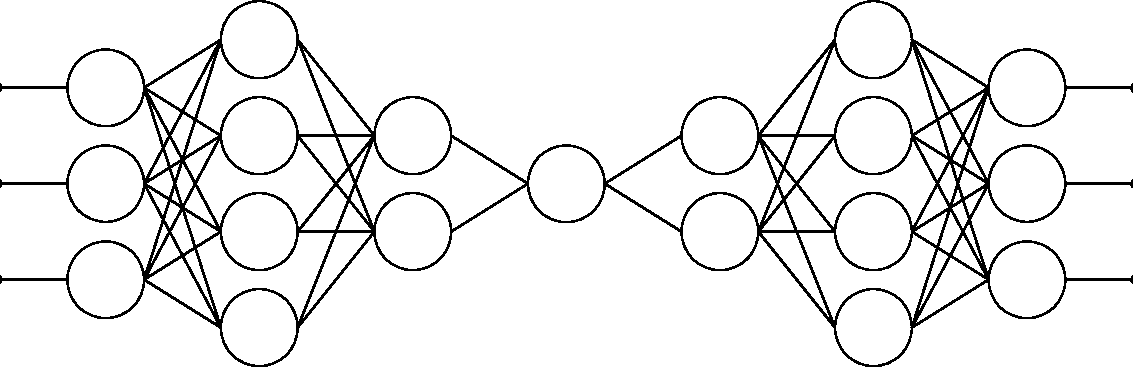
\includegraphics[width=16cm]{man-source/images/ch3/pic3-5.pdf}
	\caption{Глубокий автоэнкодер}
	\label{fig:autoencoder}
\end{figure}

Результаты обучения показаны в таблице \ref{table:data_compressing}. Здесь MSE -- среднеквадратичная ошибка на выборке обучения, MS -- среднеквадратичная ошибка на тестовой выборке для проверки обобщающей способности сети. Количество примеров в тестовой выборке -- 1000. Скорость обучения $\alpha$ -- 0.1 для классического метода обучения и 0.5 для REBA для всех экспериментов.

			\begin{table}[h]
				\caption{Сравнение методов предобучения (сжатие)}								\label{table:data_compressing}
				\centering
				\begin{tabular}{|p{4cm}|p{3cm}|p{2cm}|p{2cm}|}
					\hline
					Метод & CD-k & MSE & MS \\
					\hline
					C-RBM & 1  & 0,699 & 0,886 \\
                        \cline{2-4}
					& 5  & \textbf{0,710} & \textbf{0,932}\\
                        \cline{2-4}							
					&	10 & 0,689 & 0,916\\
					\cline{2-4}
                        &	15 & \textbf{0,688} & \textbf{0,873}\\ \hline
					REBA& 1  & \textbf{0,673} & \textbf{0,851}\\
                        \cline{2-4}
					& 5  & 0,719 & 0,966\\
                        \cline{2-4}
					&	10 & \textbf{0,677} & \textbf{0,907}\\
                        \cline{2-4}
					&	15 & 0,700 & 0,895 \\						
					\hline
				\end{tabular}			
			\end{table}	

Число эпох предобучения -- 10. Число эпох <<тонкой настройки>> нейронной сети -- 1000. Из полученных результатов видно, что использование метода предобучения REBA позволило улучшить обобщающую способность глубокого автоэнкодера для случаев CD-1 и CD-10. На рисунках \ref{f:15} и \ref{f:16} изображены оригинальные данные, на которых производилось обучение, и восстановленные из одного нелинейного компонента, используя тестовые данные. Как можно видеть, автоэнкодер восстанавливает данные из одного нелинейного компонента с хорошей точностью.

\begin{figure}[h]
	\begin{center}
		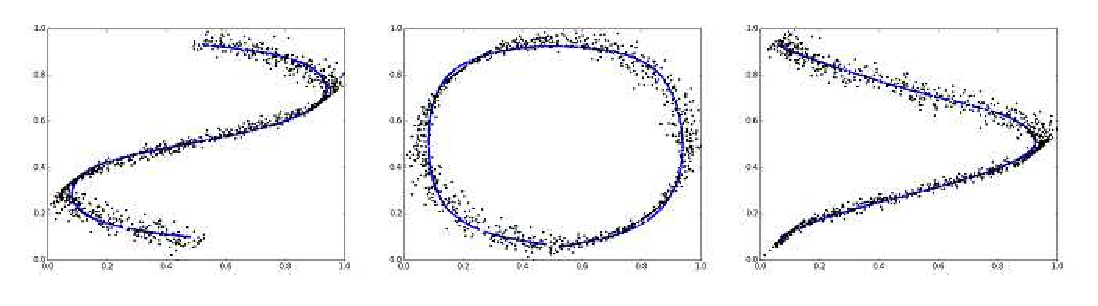
\includegraphics[width=160mm]{man-source/images/ch3/pic3-6.pdf}
		\caption{2D-изображения оригинальных и реконструированных данных}				
		\label{f:15}
	\end{center}
\end{figure}

\begin{figure}[h!]
	\begin{center}
		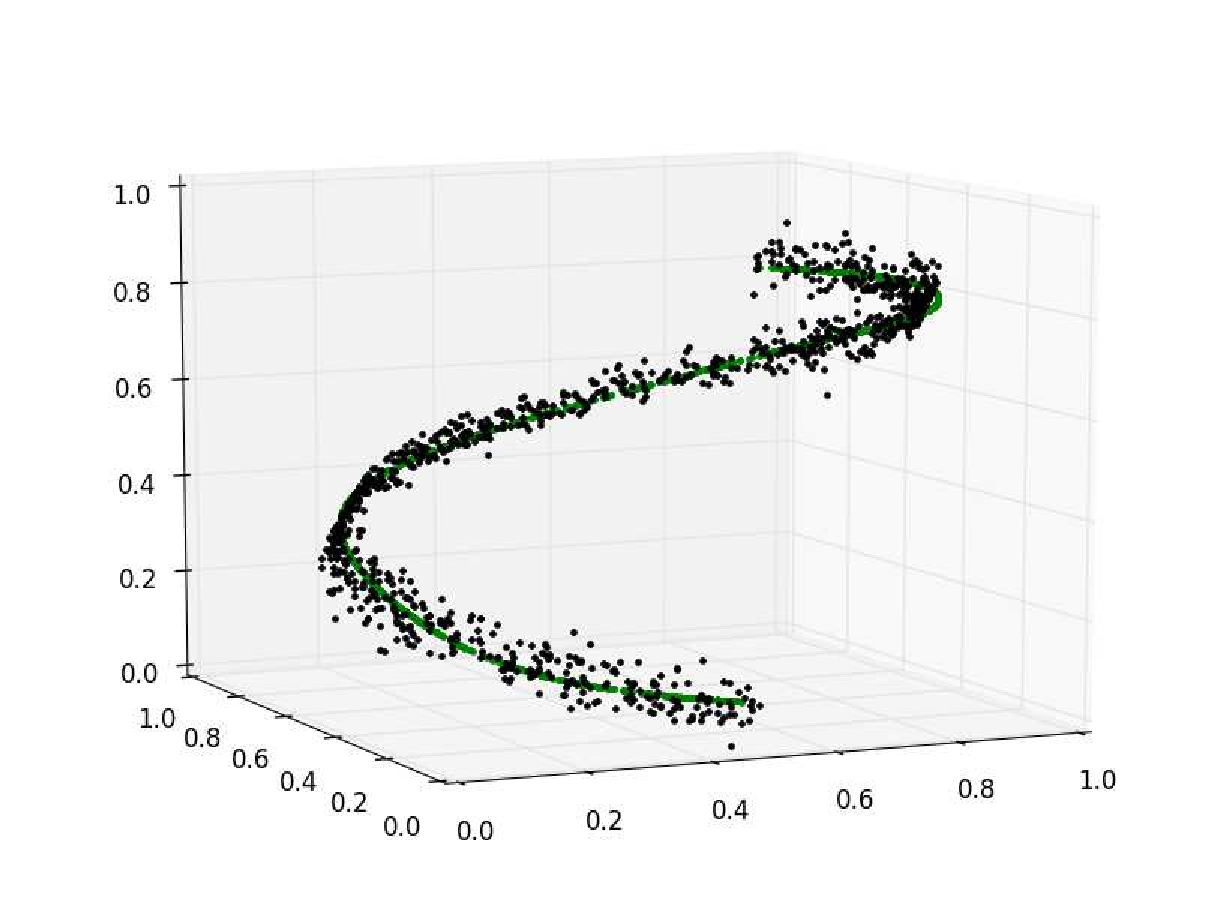
\includegraphics[width=120mm]{man-source/images/ch3/pic3-7.pdf}
		\caption{3D-изображение оригинальных и реконструированных данных}				
		\label{f:16}
	\end{center}
\end{figure}

% \section{Распознавание образов}
% \subsection{Ирисы Фишера}

% Рассмотрим решение задачи распознавания образов на примере известной выборки Фишера \cite{Fisher}. Эта выборка была представлена Рональдом Фишером в 1936 году в качестве примера для демонстрации разработанного им метода линейного дискриминантного анализа. Она включает 150 образов ирисов, относящихся к трем различным классам. Каждый образ представляет собой 4-х мерный вектор признаков.

% Отличительная особенность этой задачи в том, что один класс образов является линейно разделимым, в то время как два других -- нет (рис. \ref{fig:irises_visualize}).

% \begin{figure}[h]
% 	\begin{center}
% 		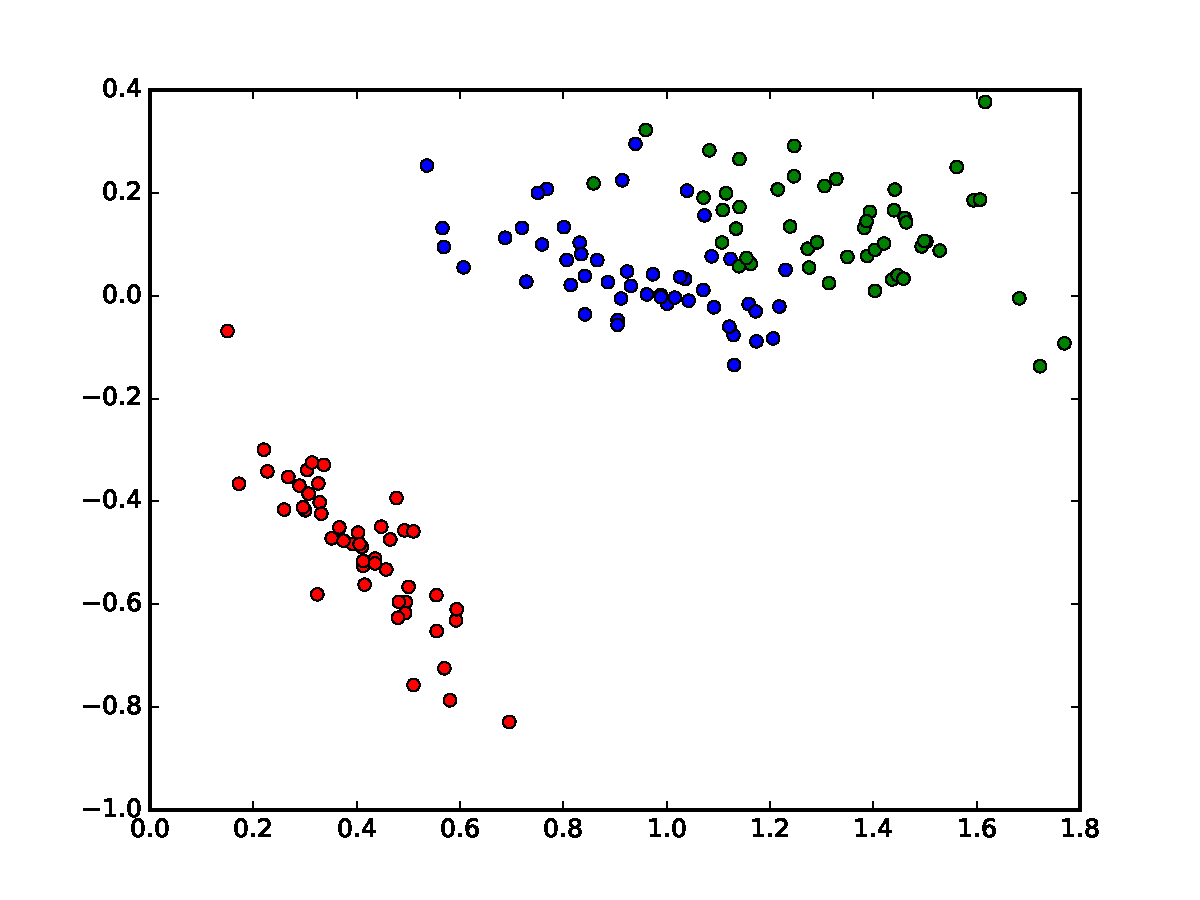
\includegraphics[width=10cm]{man-source/images/ch3/pic3-8.pdf}
% 		\caption{Визуализация образов ирисов Фишера (получена применением PCA)}				
% 		\label{fig:irises_visualize}
% 	\end{center}
% \end{figure}

% Применяя классические подходы кластеризации (например, метод k-средних), можно заметить неприемлемое качество распознавания на границах двух линейно неразделимых классов (рис. \ref{fig:kmeans})

% \begin{figure}[h]
% 	\begin{center}
% 		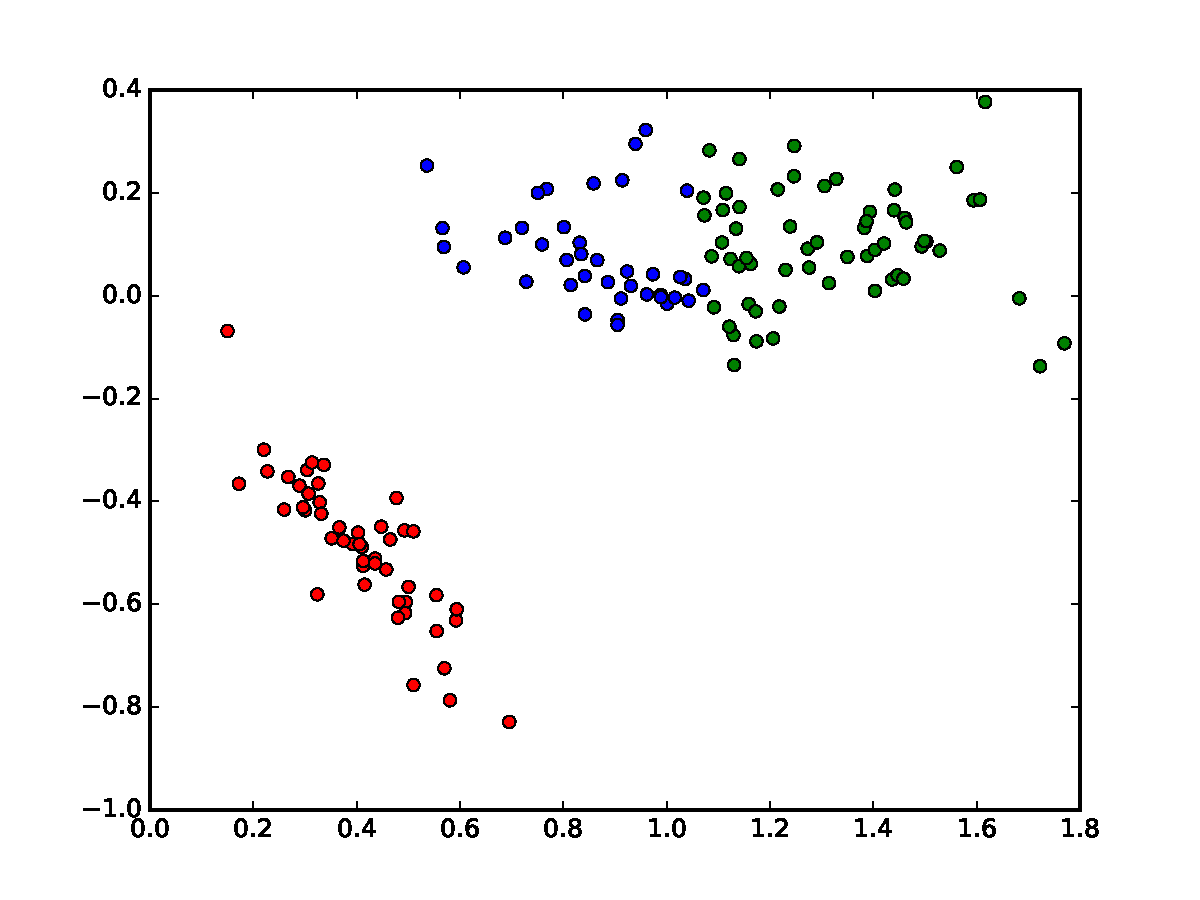
\includegraphics[width=10cm]{man-source/images/ch3/pic3-9.pdf}
% 		\caption{Кластеризация образов ирисов Фишера методом k-средних}			
% 		\label{fig:kmeans}
% 	\end{center}
% \end{figure}

% Обучим глубокую нейронную сеть для классификации образов из выборки Фишера. Для решения этой задачи воспользуемся сетью с архитектурой \textbf{4-32-16-8-3} с сигмоидными функциями активации на каждом обрабатывающем слое. 
% Другие параметры:
% \begin{itemize}
% 	\item Фаза предобучения: скорость -- 0.1 (для REBA 0.4), моментный параметр -- переменный (от 0.5 до 0.9), размер мини-батча - 5, количество эпох обучения каждого слоя -- 50.
% 	\item Фаза обучения: скорость -- 0.05 (с редуцированием, коэффициент 0.99), моментный параметр -- 0.9, размер мини-батча -- 5, количество эпох обучения -- 2000, параметр L2-регуляризации (weight decay) -- 0.00001.
% \end{itemize}

% После обучения нейронной сети нами была достигнута совокупная ошибка распознавания 99,33\%. Таким образом, неправильно распознанным остался только один образ из всей выборки (см. рис. \ref{fig:fisher_irises_results}).

% \begin{figure}[h]
% 	\begin{center}
% 		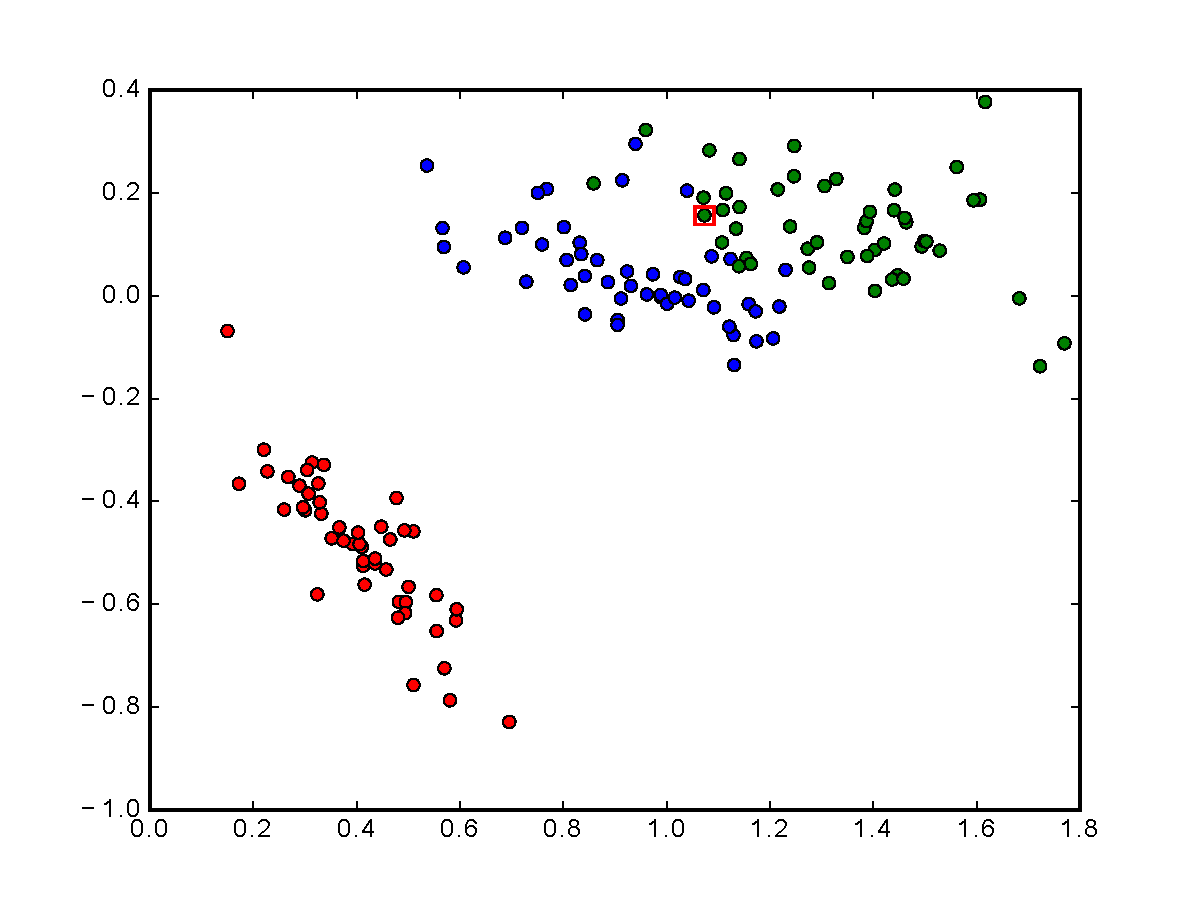
\includegraphics[width=12cm]{man-source/images/ch3/pic3-10.pdf}
% 		\caption{Результат работы обученной глубокой нейронной сети с отмеченным неправильно классифицированным образом}				
% 		\label{fig:fisher_irises_results}
% 	\end{center}
% \end{figure}

% Показательной в данном случае является эволюция среднеквадратичной ошибки после предобучения разными методами и без него (рис. \ref{fig:error_evolution}).

% \begin{figure}[h]
% 	\begin{center}
% 		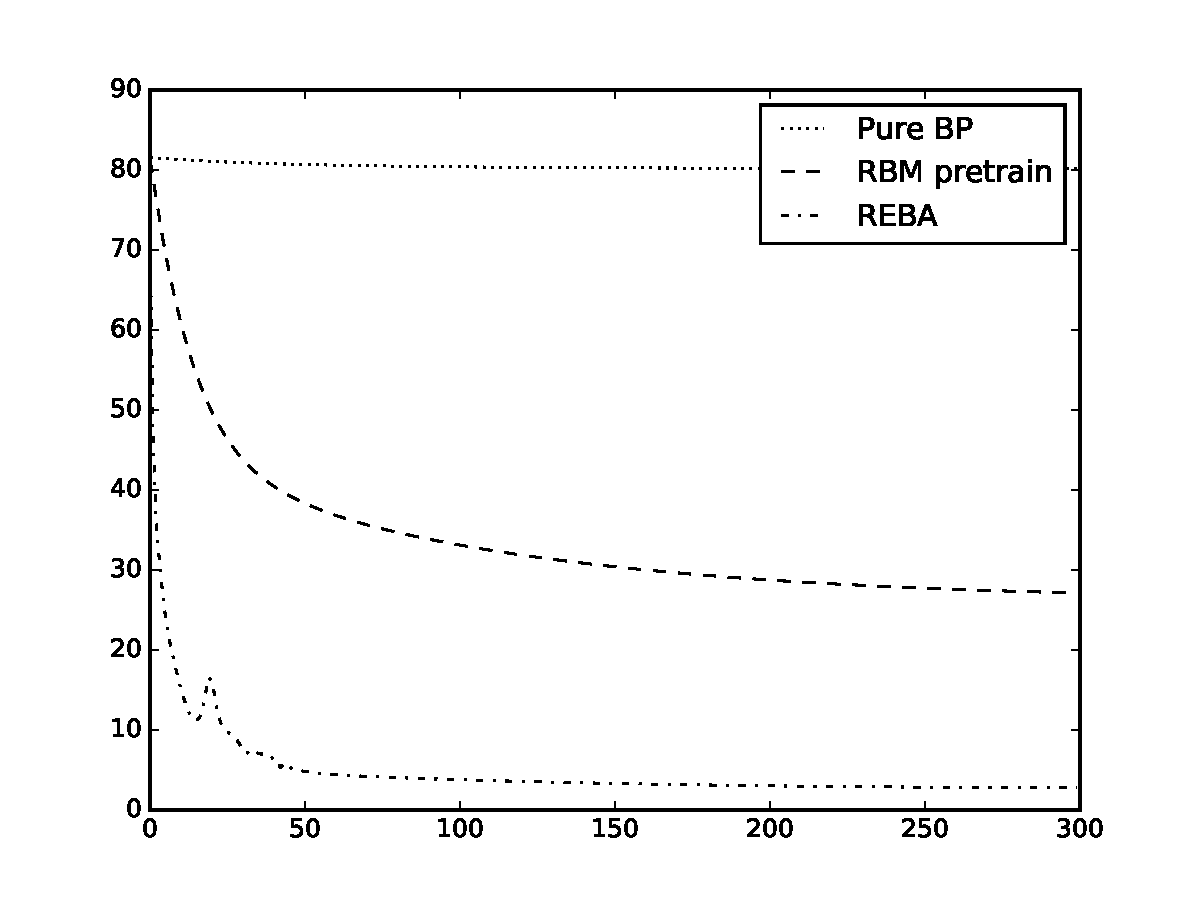
\includegraphics[width=12cm]{man-source/images/ch3/pic3-11.pdf}
% 		\caption{Эволюция ошибок обучения разными методами}	
% 		\label{fig:error_evolution}
% 	\end{center}
% \end{figure}

% Таким образом, предобучение позволяет получить хорошую начальную инициализацию весов и порогов нейронной сети, что делает последующий этап <<тонкой настройки>> методом обратного распространения ошибки значительно более продуктивным.

% \section{Гибридный алгоритм предобучения}

% При обучении нейронных сетей, как поверхностных, так и глубоких архитектур, можно использовать целевые минимизируемые функции разных видов. В главе 1 были приведены основные функции ошибок, часто применяемые на практике (\ref{MSE}, \ref{CE}).

% В различных публикациях исследуется вопрос применения обоих критериев (например, \cite{Golik}, \cite{Zhou}). При этом полученные в \cite{Golik} результаты подтверждают, что обучение классификаторов в соответствии с критерием $E_{CE}$ позволяет найти лучший локальный оптимум, чем с критерием $E_{MSE}$, применение которого приводит к быстрому <<застреванию>> в локальном оптимуме, где градиент стремится к нулю и, как результат, дальнейшее уменьшение ошибки классификации становится невозможным. 

% В \cite{Golik} исследуется вопрос применения гибридного подхода. Начиная с хорошей начальной инициализации, полученной при обучении с критерием $E_{CE}$, дальнейший процесс с $E_{MSE}$ способен дать лучший результат, чем при обучении только с критерием $E_{CE}$. 

% % При этом полученные авторами результаты подтверждают, что если обучение вначале будет вестись в соответствии с правилами по формуле $E_{CE}$, а затем несколько эпох - по формуле $E_{MSE}$, итоговая обобщающая способность сети будет выше, чем при обучении только с использованием $E_{CE}$.

% Таким образом, с учетом ранее доказанных теорем, может быть сформулирован гибридный вариант предобучающего алгоритма.

\section{Классификация}

\subsection{Критерий оценки результатов классификации}

Для оценки качества решения задачи классификации применялся следующий подход. Вначале определялся $k$-тый нейрон, выходное значение которого было максимальным для заданного образа $s$ (данное число соответствует метке класса, получаемого моделью):

\begin{equation}
  k_s = \arg \max_j y_j^s.
\end{equation}

Затем получившееся значение сравнивалось с эталонными значениями и количество совпадений суммировалось для всех образов:

\begin{equation}
  S = \sum_{s=1}^{L} [k_s = e_s],
\end{equation}
где $[x]$ -- нотация (скобка) Айверсона для высказывания $x$,\\
$L$ -- общее количество образов из оцениваемого множества,\\
$e_s$ -- эталонное значение, метка класса, соответствующая $s$-тому образу.

Значения нотации Айверсона могут быть получены по следующей формуле:

\begin{equation*}
    [x] = 
    \begin{cases}
        1, & \text{x is True} \\
        0, & \text{x is False}.
    \end{cases}
\end{equation*}

Таким образом, общая эффективность на тестовой выборке может быть получена по следующей формуле:

\begin{equation}
\text{Efficiency} = \frac{S}{L} * 100\%.
\end{equation}

\subsection{Решение простейшей задачи классификации}

Рассмотрим решение задачи классификации на примере известной выборки Фишера \cite[c.~180]{Fisher}. Эта выборка была представлена Рональдом Фишером в 1936 году в качестве примера для демонстрации разработанного им метода линейного дискриминантного анализа.

Отличительная особенность этой задачи в том, что один класс образов из данной выборки является линейно разделимым, в то время как два других -- нет (рисунок~\ref{fig:irises_visualize}).

\begin{figure}[h]
	\begin{center}
		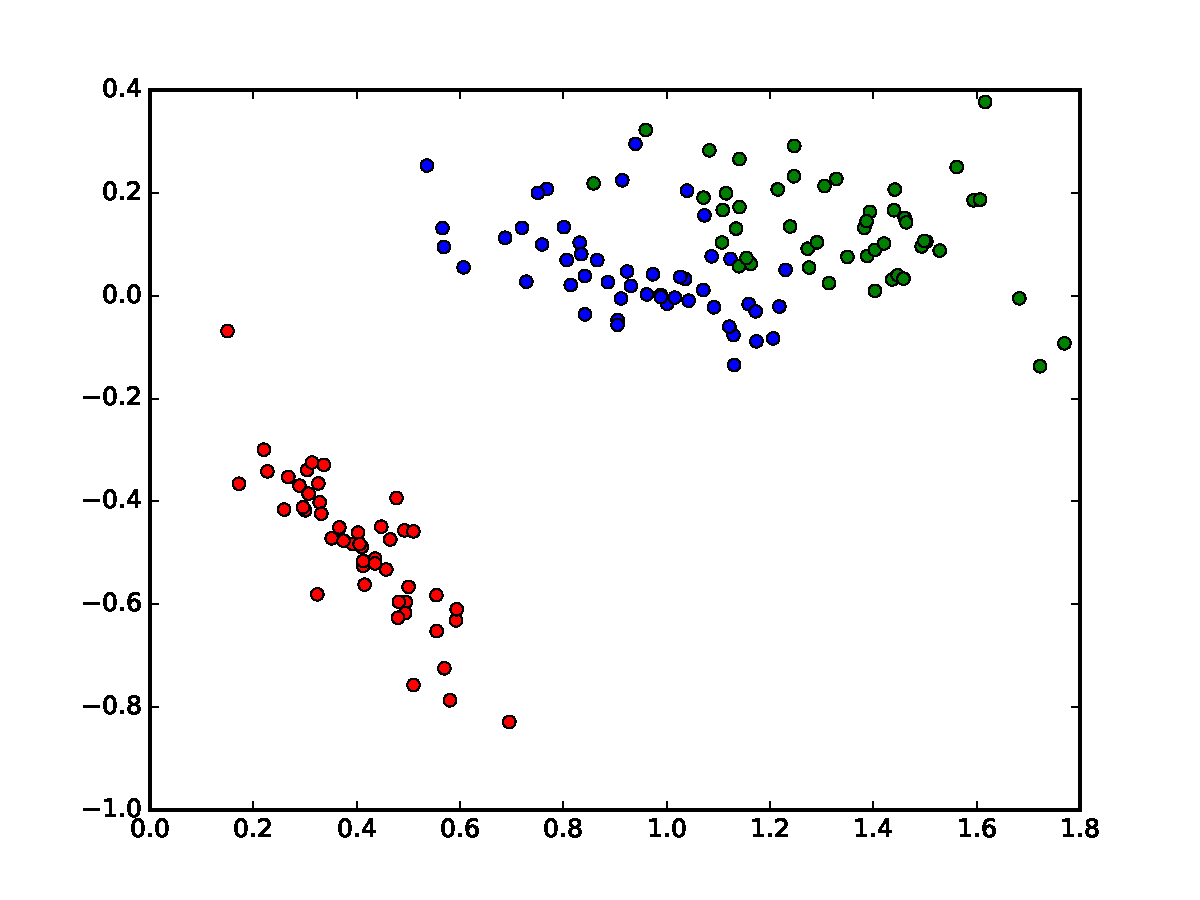
\includegraphics[width=10cm]{man-source/images/ch3/pic3-8.pdf}
		\caption{Визуализация образов ирисов Фишера (получена применением метода PCA)}				
		\label{fig:irises_visualize}
	\end{center}
\end{figure}

Применяя классические подходы кластеризации (например, метод k-средних), можно заметить неприемлемое качество распознавания на границах двух линейно неразделимых классов (рисунок \ref{fig:kmeans}).

\begin{figure}[h]
	\begin{center}
		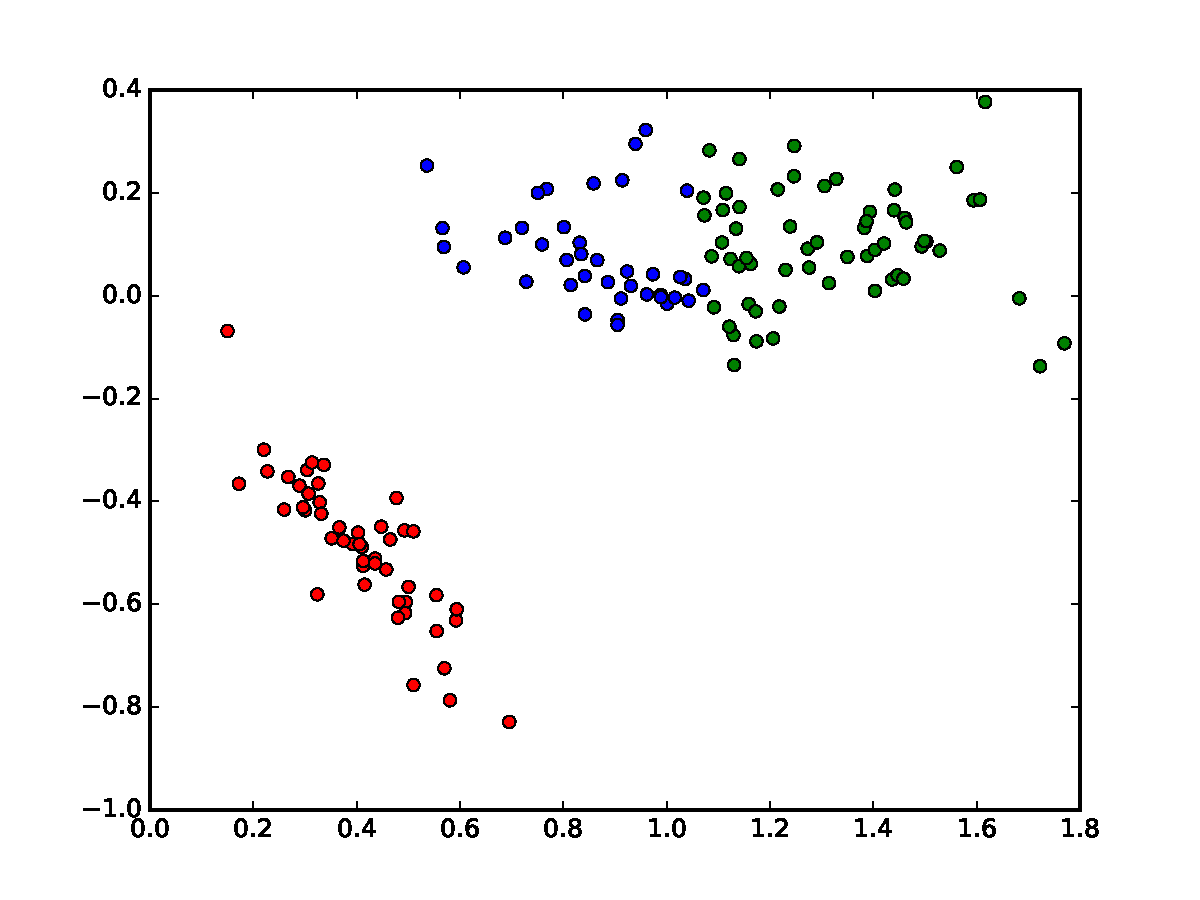
\includegraphics[width=10cm]{man-source/images/ch3/pic3-9.pdf}
		\caption{Кластеризация образов ирисов Фишера методом k-средних}			
		\label{fig:kmeans}
	\end{center}
\end{figure}

Для решения этой задачи была использована сеть с архитектурой \textbf{4-32-16-8-3} с сигмоидными функциями активации на каждом обрабатывающем слое \cite{22-A}. 
Другие параметры:
\begin{itemize}
	\item фаза предобучения: скорость -- 0.1 (для REBA 0.4), моментный параметр -- переменный (от 0.5 до 0.9), размер мини-батча - 5, количество эпох обучения каждого слоя -- 50;
	\item фаза обучения: скорость -- 0.05 (с редуцированием, коэффициент 0.99), моментный параметр -- 0.9, размер мини-батча -- 5, количество эпох обучения -- 2000, параметр L2-регуляризации (weight decay) -- 0.00001.
\end{itemize}

После обучения нейронной сетью была достигнута совокупная ошибка распознавания 99,33\%. Таким образом, неправильно распознанным остался только один образ из всей выборки (рисунок \ref{fig:fisher_irises_results}).

\begin{figure}[h]
	\begin{center}
		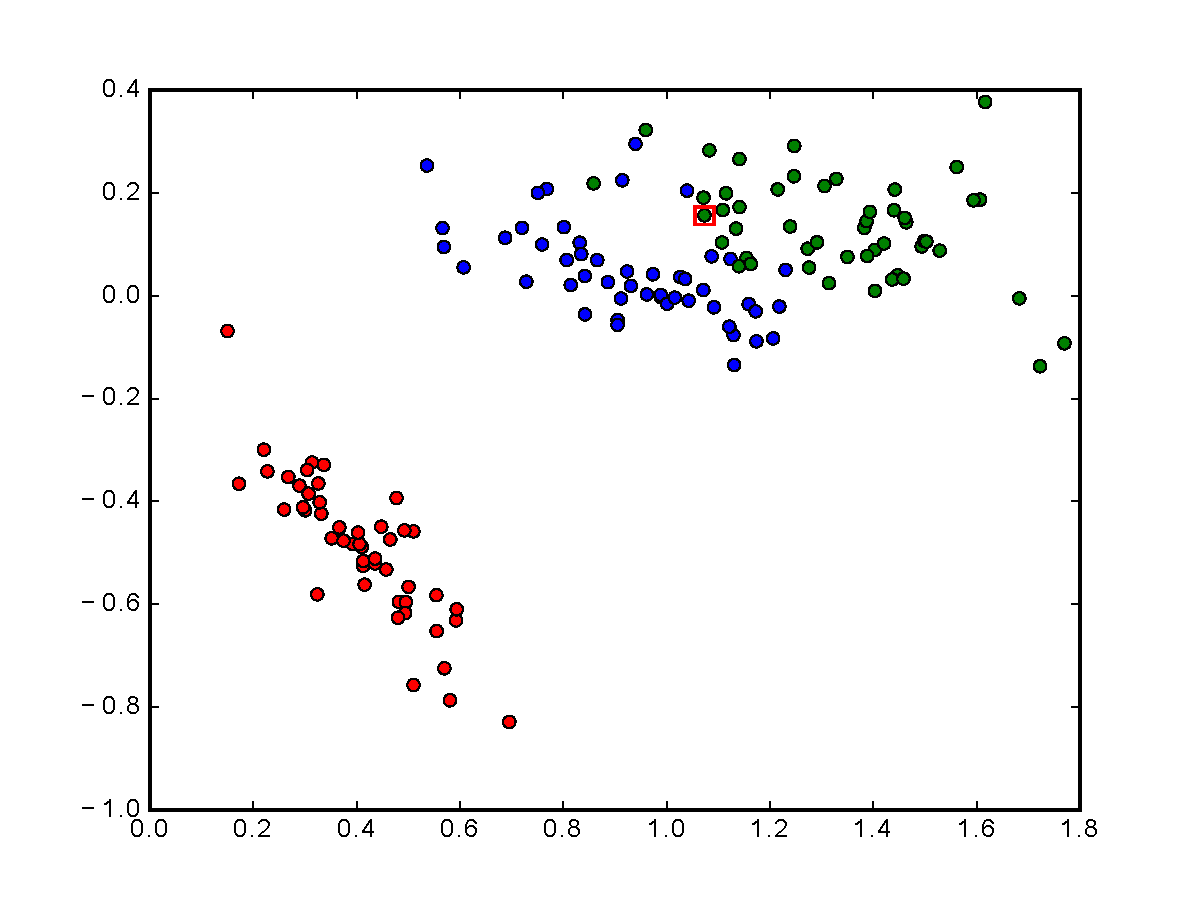
\includegraphics[width=12cm]{man-source/images/ch3/pic3-10.pdf}
		\caption{Результат работы обученной нейронной сети с отмеченным неправильно классифицированным образом}				
		\label{fig:fisher_irises_results}
	\end{center}
\end{figure}

Эволюция среднеквадратичной ошибки после предобучения разными методами и без предобучения изображена на рисунке \ref{fig:error_evolution}.

\begin{figure}[h]
	\begin{center}
		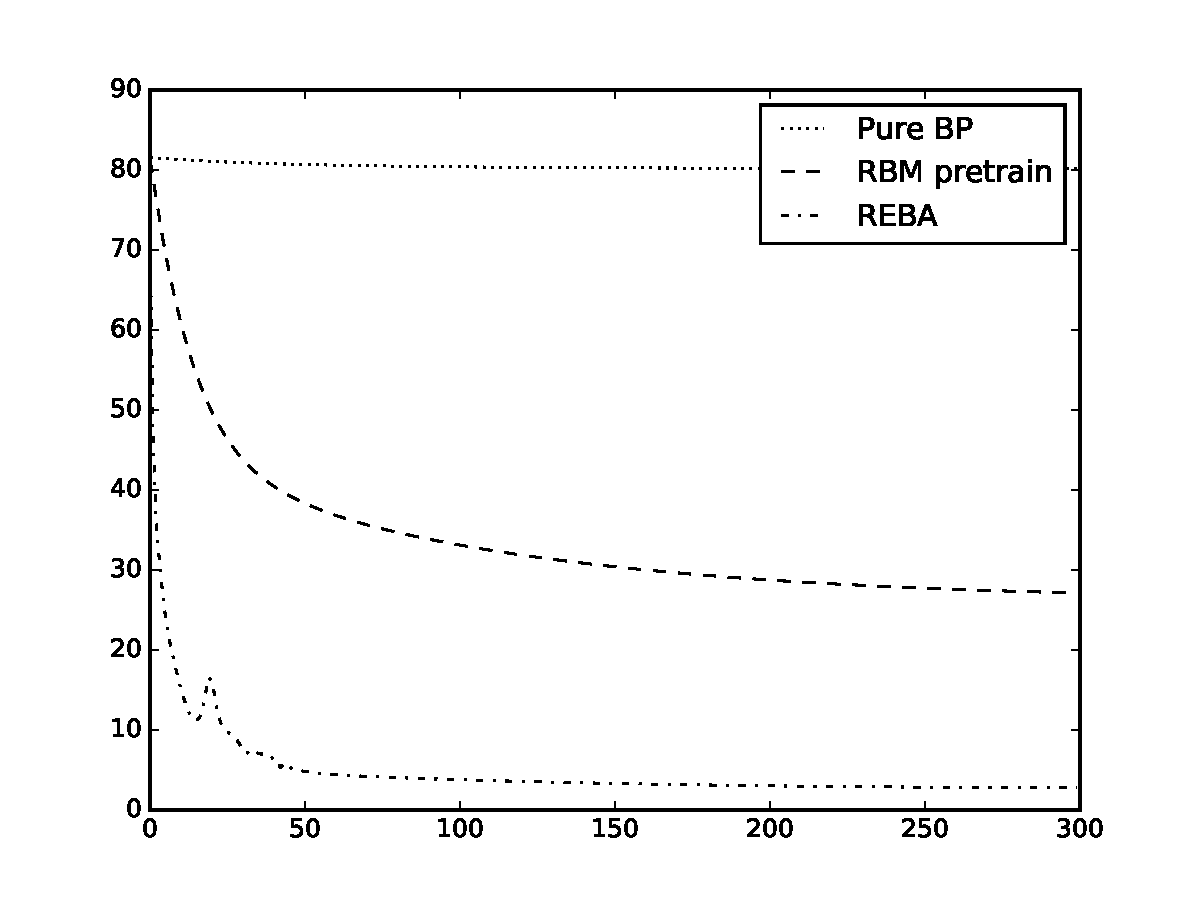
\includegraphics[width=12cm]{man-source/images/ch3/pic3-11.pdf}
		\caption{Эволюция ошибок обучения разными методами}	
		\label{fig:error_evolution}
	\end{center}
\end{figure}

Как видно из представленного графика, предобучение позволяет получить хорошую начальную инициализацию весов и порогов нейронной сети, что делает последующий этап <<тонкой настройки>> методом обратного распространения ошибки более эффективным.

\subsection{Описание применяемых выборок}

С практической точки зрения (и в соответствии с объектом исследования) наибольший интерес представляют выборки графических образов.

Задача распознавания графических образов является одной из основных в области компьютерного зрения. В настоящий момент <<золотым стандартом>> выборок, применяемых для оценки эффективности моделей выступают MNIST, CIFAR-10 и CIFAR-100. %На этих выборках уже получены хорошие результаты по достигнутой эффективности моделей. Однако, нужно отметить, что для ряда подходов, для которых получены лучшие результаты при тестировании на данных выборках, используются аугментированные (т.е. измененные данные), которые позволяют значительно увеличить размерность обучающей выборки. Перед нами стояла задача сравнения методов предобучения, без достижения state-of-art результатов для выборок, поэтому методы аугментации данных не применялись.

Выборка MNIST (Mixed National Institute of Standards and Technology database) является классической при тестировании систем распознавания образов, а также широко используемой для обучения и тестирования алгоритмов машинного обучения. Она сформирована как подмножество более крупной оригинальной выборки NIST \cite{mnist}, изображения из которого были дополнительно предобработаны (путем изменения размера и центрирования). 

Выборка MNIST состоит из 60000 образов для обучения и 10000 образов для тестирования. Каждый образ представляет собой изображение цифры размером 28Х28 пикселей в градациях серого цвета. На рисунке \ref{fig:mnist_example} изображен фрагмент базы изображений MNIST с наиболее труднораспознаваемыми цифрами.

\begin{figure}[h]
	\begin{center}
		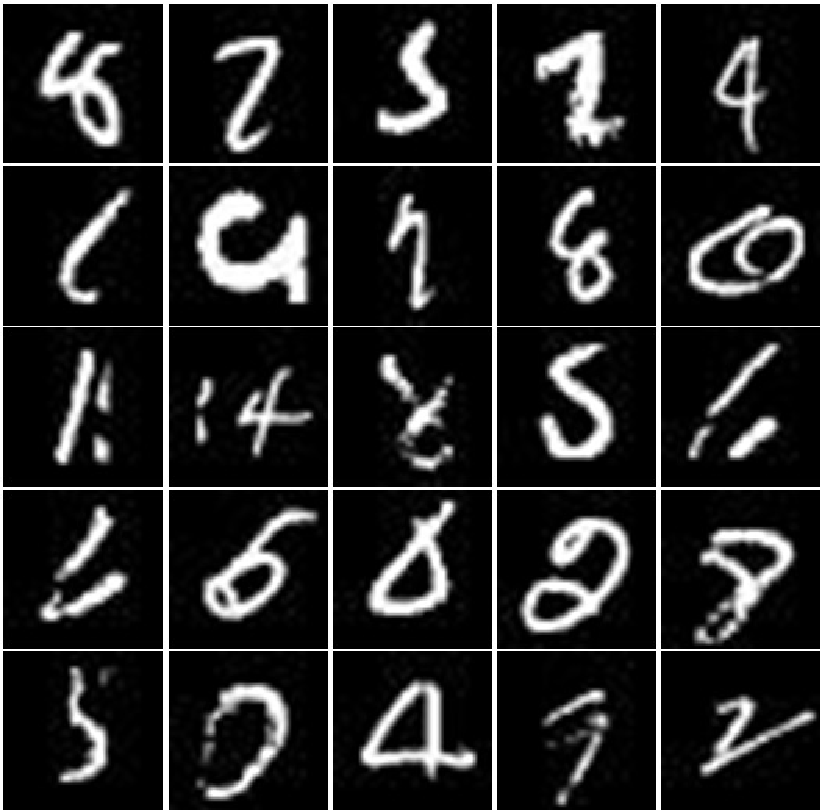
\includegraphics[width=8cm]{man-source/images/ch3/pic3-12.pdf}
		\caption{Фрагмент базы изображений MNIST}		
		\label{fig:mnist_example}
	\end{center}
\end{figure}

Выборка CIFAR-10 \cite[c.~3]{krizhevsky2009learning} является подмножеством выборки Tiny Images \cite[c.~1958]{torralba2008} и включает в себя 60.000 цветных изображений технических средств и живых существ, принадлежащий 10 различным классам (рисунок~\ref{fig:cifar_dataset}) по 6.000 изображений на каждый класс. Каждое изображение имеет размер 32Х32 пикселя.

\begin{figure}[h!]
	\begin{center}
		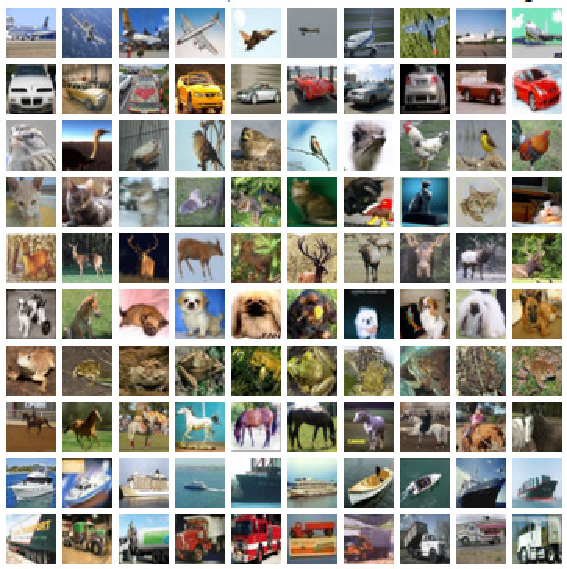
\includegraphics[width=10cm]{man-source/images/ch3/pic3-2.pdf}
		\caption{Фрагмент базы изображений CIFAR-10}				
		\label{fig:cifar_dataset}
	\end{center}
\end{figure}

Выборка CIFAR-100 идентична выборке CIFAR-10 по параметрам изображений, которые в нее включены, но отличается количеством представленных классов изображений (в этой выборке общее количество классов составляет 100). Общая размерность выборки составляет также 60.000~изображений, по 600 изображений на каждый класс.

Выборки CIFAR-10 и CIFAR-100 разделены авторами на обучающую и тестовую подвыборки (объемом 50.000 и 10.000 изображений соответственно).

%Выполнение экспериментов с использованием выборок большого размера занимает достаточно продолжительное время. Эта проблема может быть решена проведением расчетов с использованием видеокарт nVidia, поддерживающих технологию CUDA (например, ускорителей A100 или V100, доступных при использовании сервиса Google Colab \cite{googlecolab}). Существуют другие способы ускорения расчетов, производимых при обучении нейронной сети, например, использование вычислительных кластеров \cite{n16}.

%Количество входов обучаемой НС определялось размерами образов из базы MNIST (784), количество слоев и нейронов в каждом слое выявлялось экспериментальным путем. На каждом слое использовалась сигмоидная функция активации. 
\textbf{Замечание об используемых ресурсах.} Выполнение экспериментов с глубокими нейронными сетями даже при условии использования выборок среднего размера занимает продолжительное время и требует наличия значительных вычислительных ресурсов. Важными аппаратными ресурсами, влияющими на вычислительный процесс и потенциальными источниками аварийного завершения программы, становятся оперативная память и количество обрабатывающих элементов в случае использования графических ускорителей. В данной работе проблема наличия данных ресурсов была частично решена использованием сервиса Google Colab \cite{googlecolab}. Данный сервис предоставляет доступ к видеоускорителям A100 и V100, производительности которых оказалось достаточно для проведения всех расчетов. Существуют другие способы ускорения расчетов, производимых при обучении нейронной сети, например, использование вычислительных кластеров \cite[c.~701]{n16}. % проведением расчетов с использованием видеокарт nVidia, поддерживающих технологию CUDA (нами использовались ускорители A100 или V100, доступные при использовании сервиса Google Colab \cite{googlecolab}). Существуют другие способы ускорения расчетов, производимых при обучении нейронной сети, например, использование вычислительных кластеров \cite{n16}.

\subsection{Параметры вычислительного эксперимента и результаты}

В качестве целевой модели для решения задачи распознавания изображений из выборки MNIST была выбрана сверточная нейронная сеть с параметрами, представленными в таблице \ref{table:mnist_conv_model}.

\begin{table} [!h]
  \caption{MNIST: основные параметры используемой модели}\label{table:mnist_conv_model}
\centering
\begin{tabular}{| p{7cm} | p{8cm} |}
  \hline
    \textbf{Параметр} & \textbf{Значение}\\
    \hline
    Архитектура & 40Х5Х5 -- 40Х5Х5 -- 640Х320 -- 320Х160 -- 160Х10\\
    \hline
    Функция активации & ReLU \\
    \hline
    Функция активации на последнем слое & Softmax \\
    Начальная инициализация параметров & Нормальное распределение \\
    \hline
\end{tabular}
\end{table}

\textbf{Пояснение по описанию используемых архитектур НС}. В данной работе используется следующая нотация для описания архитектур НС: 
\begin{easylist}
  & для полносвязных слоев \textit{N} x \textit{M}, где \textit{N} обозначает количество входных нейронов слоя, а \textit{M} -- количество выходных нейронов;  
  & для сверточных слоев \textit{K} x \textit{S} x \textit{S}, где \textit{K} обозначает количество ядер свертки в соответствующем слое, a \textit{S} x \textit{S} -- размерность ядра свертки.
\end{easylist}
При этом для полносвязных слоев используется сокращенная форма нотации, обозначающая количество нейронов в каждом слое, например, нотация \textbf{784-100-100-10}, где 784 -- это число нейронов в первом (распределяющем) слое, 100 -- число нейронов во втором слое и так далее. 

Как видно из представленной выше таблицы, использовалась архитектура с 5 обрабатывающими слоями, 2 из которых сверточные, а 3 -- полносвязные. При этом общее число параметров модели составило 299.170.

В качестве функции активации использовалась функция ReLU на всех слоях сети, за исключением последнего слоя, на котором применялась softmax-функция. Использование ReLU позволило варианту обучения без предобучения начать процесс и завершить его с приемлемым значением эффективности.

В таблице \ref{table:mnist_comparing_params} приведены основные используемые параметры обучения.

Помимо классического и предложенного методов предобучения в ходе проведения экспериментов был протестирован подход, при котором первый слой нейросетевой модели предобучается с использованием классического метода обучения RBM, а все прочие слои, кроме последнего классифицирующего -- с использованием предлагаемого подхода REBA. Будем обозначать такой вариант предобучения как гибридный (HREBA).

Эксперименты проводились с одной и той же начальной инициализацией параметров для всех методов серией в 10 попыток, получаемые результаты затем усреднялись. В ходе эксперимента сравнивались четыре основных варианта обучения: 
\begin{easylistNum}
    & BP -- обучение без предобучения; 
    & REBA -- обучение с предобучением (предлагаемый подход); 
    & HREBA -- обучение с предобучением (гибридный подход);
    & C-RBM -- обучение с классическим методом предобучения).
\end{easylistNum}

\begin{table} [!h]
  \caption{MNIST: основные параметры обучения}\label{table:mnist_comparing_params}
\centering
\begin{tabular}{| p{3cm} | p{6cm} | p{2.5cm} |}
  \hline
    \textbf{Этап} & \textbf{Параметр} & \textbf{Значение}\\
    \hline
    Предобучение & Скорость обучения & 0,000125\\
    \cline{2-3}
    & Размер мини-батча & 128 \\
    \cline{2-3}
    & Моментный параметр & [0,5; 0,9] \\
    \cline{2-3}
    & Количество эпох обучения & 30\\
    \hline
    Обучение & Скорость обучения & 0,001\\
    \cline{2-3}
    & Размер мини-батча & 128 \\
    \cline{2-3}
    & Моментный параметр & 0,9 \\
    \cline{2-3}
    & Количество эпох обучения & 50\\
    \hline
\end{tabular}
\end{table}

В результате были получены показатели эффективности для вышеперечисленных методов, представленные в таблице \ref{table:mnist_results}.

\begin{table} [!h]
  \caption{MNIST: результаты обучения}\label{table:mnist_results}
\centering
\begin{tabular}{| p{6cm} | p{6cm} |}
  \hline
    \textbf{Метод обучения} & \textbf{Эффективность, \%}\\
    \hline
    BP & 99.367\\
    \hline
    REBA & 99.371\\
    \hline
    HREBA & \textbf{99.458}\\
    \hline
    C-RBM & 99.447\\
    \hline
\end{tabular}
\end{table}

Как видно из представленных результатов, лучший средний показатель был достигнут гибридным методом HREBA, сочетающим в себе предобучение классическим и предложенным подходом, при этом максимальная эффективность была получена этим же методом и составила \textbf{99.53} \%.

При проведении экспериментов с выборками CIFAR-10 и CIFAR-100 использовалась модель с архитектурой, представленной в таблице \ref{table:cifar_comparison_params}.

Для выборки CIFAR-100 изменения в архитектуре модели коснулись только последнего слоя (вместо 10 выходных нейронов использовалось 100 -- по количеству классов в данной выборке).

\begin{table}[!h]
    \caption{CIFAR-10/CIFAR-100: основные параметры используемых моделей}\label{table:cifar_comparison_params}
    \begin{tabular}{|p{7cm}|p{8cm}|}
        \hline
        \textbf{Параметр} & \textbf{Значение}\\
        \hline
        Архитектура & 64Х5Х5 -- 32Х5Х5 -- 800Х128 -- 128Х10/100\\
        \hline
        Функция активации & ReLU - Tanh - ReLU \\
        \hline
        Функция активации на последнем слое & Softmax \\
        \hline
        Начальная инициализация параметров & Нормальное распредение \\
        \hline
        Общее число параметров модели & 159.914
        \\
        \hline
    \end{tabular}
\end{table}

В результате были получены показатели эффективности для вышеперечисленных методов, представленные в таблице \ref{table:cifar_10_results} (для выборки CIFAR-10) и \ref{table:cifar_100_results} (для выборки CIFAR-100).

\begin{table} [!h]
  \centering
  \caption{CIFAR-10: результаты обучения}\label{table:cifar_10_results}
  \begin{tabular}{| p{6cm} | p{6cm} |}
    \hline
      \textbf{Метод обучения} & \textbf{Эффективность, \%}\\
      \hline
      BP & 69.74\\
      \hline
      REBA & 71.20\\
      \hline
      HREBA & \textbf{71.59}\\
      \hline
      C-RBM & 71.51\\
      \hline
  \end{tabular}
\end{table}

Лучший результат был получен методом HREBA и составил \textbf{72.32\%}.

\begin{table} [!h]
  \centering
  \caption{CIFAR-100: результаты обучения}\label{table:cifar_100_results}
  \begin{tabular}{| p{6cm} | p{6cm} |}
    \hline
      \textbf{Метод обучения} & \textbf{Эффективность, \%}\\
      \hline
      BP & 36.83\\
      \hline
      REBA & 38.9\\
      \hline
      HREBA & \textbf{39.86}\\
      \hline
      C-RBM & 39.71\\
      \hline
  \end{tabular}
\end{table}

Лучший результат также был получен методом HREBA и составил \textbf{40.26\%}.

% Мы использовали следующие параметры обучения: скорость обучения -- 0,1 для REBA и 0,2 для классического метода RBM, размер мини-батча -- 100, количество эпох предобучения -- 10, количество эпох <<тонкой>> настройки -- 100. Также мы использовали параметр регуляризации L2, равный 0,00001.

% Результаты экспериментов представлены в таблице \ref{table:tbl2}. \textbf{MSE} определяет ошибку обучения, \textbf{MS} -- ошибку обобщения, \textbf{Ошибка, \%}, \% -- процент ошибочно распознанных изображений, \textbf{К-во эпох} -- число эпох для классического и гибридного метода предобучения.

% \begin{table}[H]
% 	\caption{Сравнение методов предобучения (MNIST)}
% 	\label{table:tbl2}
% 	\centering
% 	\begin{tabularx}{\hsize}{| c | c | c | c | X |}
% 		\hline
% 		\textbf{Метод} & \textbf{MSE} & \textbf{MS} & \textbf{Ошибка, \%} & \textbf{Кол-во эпох}\\
% 		\hline
% 		Classic RBM & 6,178e-6  & 0,0235 & 1,23 & 10 \\
% 		\hline
% 		Hybrid REBA (9+1) & 5,962e-6 & 0,0224 & \textbf{1,09} & 9+1 \\										
% 		\hline
% 	\end{tabularx}			
% \end{table}	

% Необходимо отметить, что нейронная сеть обученная на полной выборке из базы MNIST, ошибается на образах, многие из которых трудноразличимы даже для человеческого глаза (рис. \ref{fig:incorrect_recognized_samples})

% \begin{figure}[h]
% 	\begin{center}
% 		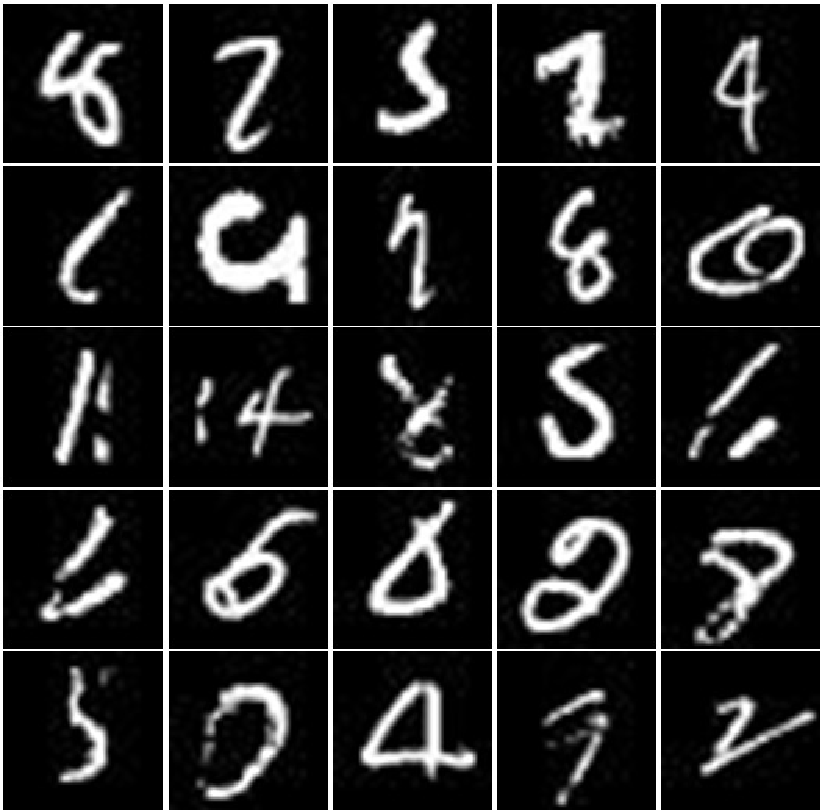
\includegraphics[width=8cm]{man-source/images/ch3/pic3-12.pdf}
% 		\caption{Образы, некорректно распознанные НС}		
% 		\label{fig:incorrect_recognized_samples}
% 	\end{center}
% \end{figure}

% \section{Визуализация данных}

% Для иллюстрации производительности метода REBA мы провели эксперименты по визуализации данных выборки MNIST. Для отображение 784-мерных данных, соответствующих количеству пикселей в исходном выражении нами использовался глубокая автоассоциативная сеть с архитектурой 784-500-500-250-10-2. Для всех слоев, за исключением среднего слоя, использовалась сигмоидная функция активации. На среднем слое применялась линейная функция. 

% Вначале выполнялось предобучение в соответствии с <<жадным>> послойным алгоритмом. Затем выполнялось <<разворачивание>> сети в полную архитектуру и производилась <<тонкая>> настройка параметров. Для предобучения использовались следующие параметры: скорость обучения -- 0.2 (REBA), скорость обучения для среднего слоя -- 0.001.

% Визуализация для первых 5000 образов из тестовой выборки представлена на рис. \ref{fig:mnist_dataset_visualize}

% \begin{figure}[ht]
% 	\centering
% 	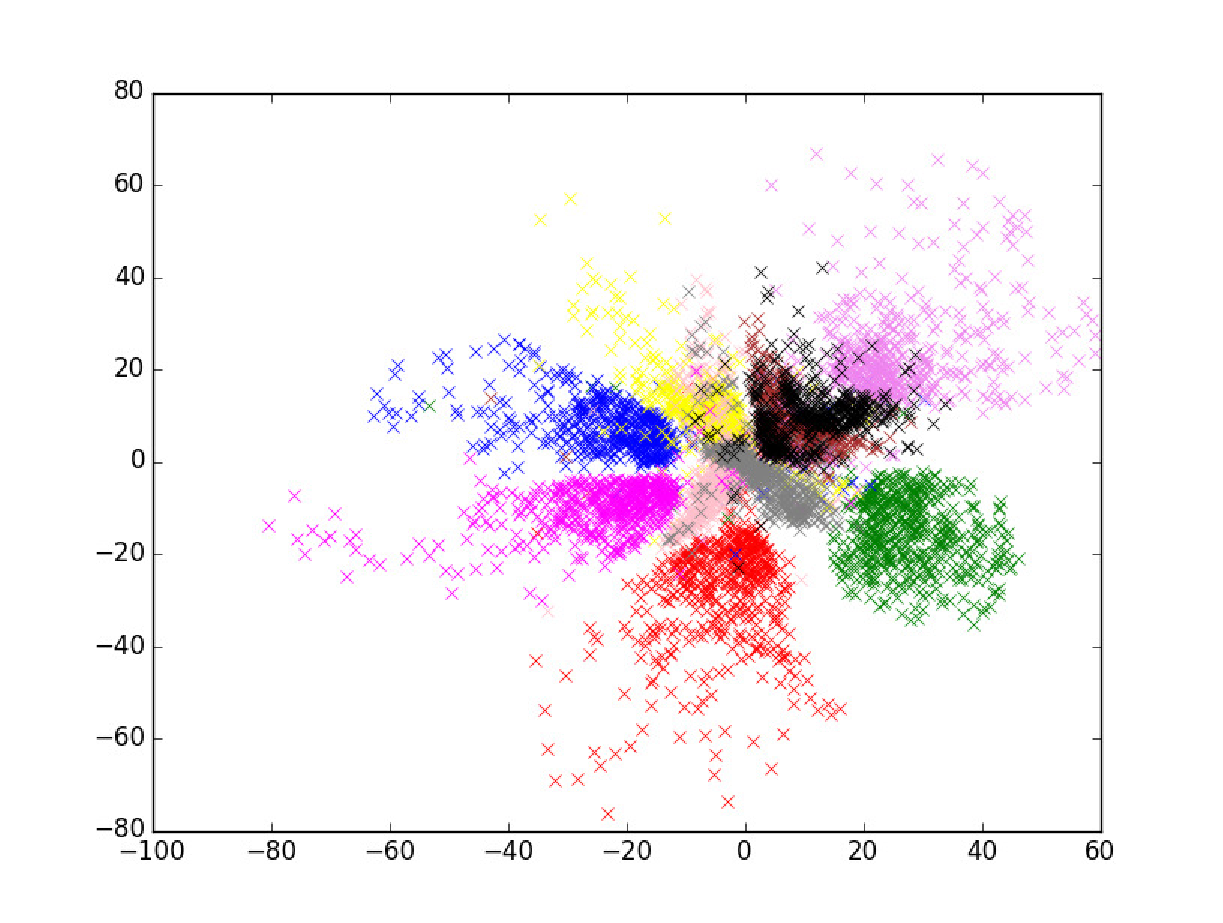
\includegraphics[width=16cm]{man-source/images/ch3/pic3-1.pdf}
% 	\caption{Визуализация рукописных цифр из базы MNIST}
% 	\label{fig:mnist_dataset_visualize}
% \end{figure}

% На рисунке видно, что в процессе обучения выделились кластеры в 2-ном пространстве главных компонент, соответствующие каждой цифре из оригинальной выборки. Таким образом, сеть не располагая информацией о каких-либо метках для исходных данных, смогла выделить области наибольшего подобия.

% \section{Семантическое кодирование}

% \subsection{Постановка задачи}
% В качестве обучающей выборки для решения задачи построения бинарных семантических кодов изображений нами была использована база CIFAR-10.  Данная выборка предоставляет богатый материал для выявления семантических особенностей \cite{n17}. Она включает в себя 50.000 изображений технических средств и живых существ, принадлежащий 10 различным классам (рис. \ref{fig:cifar_dataset}). Каждое изображение имеет размер 32Х32 пикселя.

% Помимо этого, CIFAR-10 включает тестирующую выборку, состоящую из 10.000 изображений.

% \begin{figure}[h]
% 	\begin{center}
% 		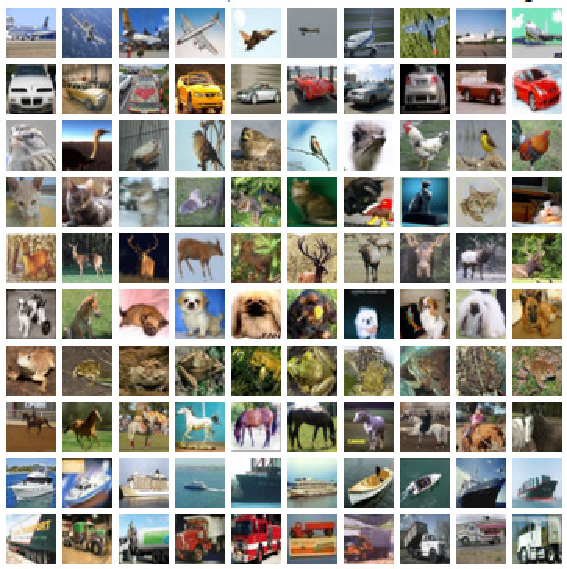
\includegraphics[width=12cm]{man-source/images/ch3/pic3-2.pdf}
% 		\caption{Фрагмент базы изображений CIFAR-10}				
% 		\label{fig:cifar_dataset}
% 	\end{center}
% \end{figure}

% Семантическое кодирование (хеширование) относится к более сложному и не менее важному типу задач, решение которого позволяет сформировать бинарный код ограниченной длины, емко и однозначно описывающий изображение в редуцированном признаковом пространстве. С помощью такого преобразования можно сформировать базу изображений, представленных лишь бинарным кодом. На основе такой базы можно построить систему релевантного поиска изображений.

% \subsection{Структура сети и основные параметры обучения}
% Для решения задачи нами использовалась 11-слойная ассоциативная нейронная сеть с архитектурой 3072-4096-2048-1024-512-256-512-1024-2048-4096-3072. На среднем слое такой сети формируется вектор вещественных значений из отрезка [0, 1], элементы которого затем округляются. Таким образом формируется бинарный код изображения. Легко видеть, что таким образом может быть закодировано $2^{256}$ изображений, что более чем достаточно для базы CIFAR-10. Нами использовались все изображения из обучающей выборки указанной базы.

% Обучение проводилось в два этапа. На первом этапе предобучались соответствующие RBM, формирующие кодирующие слои сети. Исходные данные перед обучением были стандартизованы: из каждого компонента вектора изображения вычиталось его среднее значение по всем изображениям выборки и затем полученное значение делилось на стандартное отклонение по всем компонентам всех изображений. Данное преобразование определило тип первой обучаемой машины Больцмана -- линейно-бинарная RBM \cite{n4}. Остальные машины обучались как бинарные RBM.

% Каждая RBM обучалась на протяжении 100 эпох мини-батчами по 100 элементов. Для линейно-бинарной RBM использовалось скорость обучения 0,001, для бинарной -- 0,01. Помимо этого для ускорения процесса обучения использовался моментный параметр, равный 0,9.

% После проведения предобучения выполнялось обучение развернутой автоассоциативной сети методом обратного распространения ошибки. Параметры обучения: скорость -- $1e^{-6}$, количество эпох обучения -- 150, моментный параметр -- 0.9.

% После выполнения обучения, результат оценивался вычислением расстояния Хэмминга между бинарными кодами для тестового изображения и изображениями из базы (формула \ref{chemming_dist}) После этого полученный ряд значений сортировался по возрастанию для выделения наиболее релевантных результатов.

% \begin{equation}
% 	\label{chemming_dist}
% 	H(v_1,v_2) = \sum_{i=1}^{n}|v_1^i-v_2^i|
% \end{equation}

% Вычисления, производимые в процессе обучения глубокой автоассоциативной нейронной сети производились на видеокарте GTX 750 Ti и заняли приблизительно 90 минут.

% Программный код на языке программирования Python для выполнения предобучения данной сети приведен в приложении 1.

% \subsection{Результаты обучения}
% Мы протестировали нашу модель двумя способами. Первый вариант предусматривал визуальное сравнение оригинального и восстановленного изображения. Некоторые из выполненных тестов представлены на рисунке \ref{fig:restore_images_results}.

% \begin{figure}[h]
% 	\begin{center}
% 		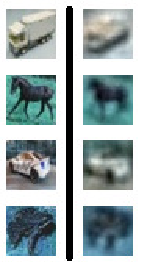
\includegraphics[width=40mm]{man-source/images/ch3/pic3-3.pdf}
% 		\caption{Оригинальные и восстановленные нейронной сетью изображения}				
% 		\label{fig:restore_images_results}
% 	\end{center}
% \end{figure}

% Второй вариант тестирования заключался в подаче на обученную автоассоциативную сеть изображения, получения его бинарного кода с промежуточного слоя сети и вычисления расстояния Хэмминга для всех остальных изображений. Отсортировав получившуюся последовательность по возрастанию, можно изучить наиболее релевантные результаты поиска (рис. \ref{fig:search_template}).

% \begin{figure}[h]
% 	\begin{center}
% 		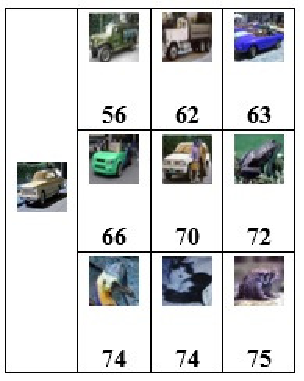
\includegraphics[width=8cm]{man-source/images/ch3/pic3-4.pdf}
% 		\caption{Поисковый шаблон и результаты поиска}				
% 		\label{fig:search_template}
% 	\end{center}
% \end{figure}

% Исходя из представленных данных, можно отметить, что с увеличением расстояния Хэмминга количество изображений того же класса, что и целевое изображение постепенно уменьшается.

\section{Редуцирование параметров НС}

% Экспериментальные исследования метода редуцирования параметров проводились на полносвязных и сверточных нейронных сетях.

Продемонстрируем эффективность предложенного подхода на примере редуцирования различных архитектур полносвязных нейронных сетей, применяемых для классификации изображений из выборок MNIST \cite{mnist}, CIFAR10 и CIFAR100 \cite[c.~3]{krizhevsky2009learning}.
Были проведены серии экспериментов, включающих различные используемые выборки, архитектуры и варианты предобучения. В рамках одной выборки и архитектуры НС текущая инициализация параметров сохранялась для возможности сравнения эффективности различных вариантов предобучающей процедуры.
Ниже для рассматриваемых выборок приведены основные параметры, включающие скорость обучения, размер мини-батча, моментный параметр и количество эпох для предобучения и <<тонкой настройки>> моделей (таблица \ref{table:reduce_training_params}).

\begin{table} [!h]
  \small
  \caption{Основные параметры обучения}\label{table:reduce_training_params}
\centering
\begin{tabular}{| p{3cm} | p{6cm} | p{2cm} |}
  \hline
    \textbf{Этап} & \textbf{Параметр} & \textbf{Значение}\\
    \hline
    Обучение & Скорость обучения & 0.05-0.1\\
    \cline{2-3}
    & Размер мини-батча & 100 \\
    \cline{2-3}
    & Моментный параметр & 0.9 \\
    \cline{2-3}
    & Количество эпох обучения & 50-100\\
    \hline
    Предобучение & Скорость обучения & 0.05-0.2\\
    \cline{2-3}
    & Размер мини-батча & 32-100 \\
    \cline{2-3}
    & Моментный параметр & [0.5, 0.9] \\
    \cline{2-3}
    & Количество эпох обучения & 10\\
    \hline
\end{tabular}
\end{table}

В результате вычислительного эксперимента были получены результаты для различных выборок, архитектур НС и значений параметра редуцирования t (таблицы \ref{table:mnist_1}-\ref{table:cifar_100}).

\begin{table} [!h]
  \small
  \caption{Результаты для сети 784-800-800-10 на выборке MNIST}\label{table:mnist_1}
\centering
\begin{tabular}{| p{2cm} | p{4cm} | p{4cm} | p{4cm} |}
  \hline
    \textbf{Тип} & \textbf{Эффективность, \%, C-RBM / REBA} & \textbf{Количество параметров, C-RBM / REBA} & \textbf{Редуцировано параметров, \%, C-RBM / REBA}\\
    \hline
    без редуц. & \textbf{98.63} / 98.33 & 1276810 / 1276810 & 0/0\\
    \hline
    t=0.2 & \textbf{98.61} / 98.27 & \textbf{233760} / 279635 & \textbf{81.69} / 78.1\\
    \hline
    t=0.5 & 98.03 / \textbf{98.05} & \textbf{32524} / 32817 & \textbf{97.45} / 97.43\\
    \hline
    t=0.8 & \textbf{97.1} / 96.48 & 17061 / \textbf{12217} & 98.66 / \textbf{99.04}\\
    \hline
\end{tabular}
\end{table}

\begin{table} [!h]
  \small
  \caption{Результаты для сети 784-1600-1600-800-800-10 на выборке MNIST}\label{table:mnist_2}
\centering
\begin{tabular}{| p{2cm} | p{4cm} | p{4cm} | p{4cm} |}
  \hline
    \textbf{Тип} & \textbf{Эффективность, \%, C-RBM / REBA} & \textbf{Количество параметров, C-RBM / REBA} & \textbf{Редуцировано параметров, \%, C-RBM / REBA}\\
    \hline
    wr & \textbf{98.76} / 98.37 & 5747210 / 5747210 & 0/0\\
    \hline
    t=0.2 & 98.51 / \textbf{98.55} & \textbf{710734} / 781103 & \textbf{87.63} / 86.41\\
    \hline
    t=0.5 & 98.01 / \textbf{98.03} & 54709 / \textbf{43867} & 99.05 / \textbf{99.24}\\
    \hline
    t=0.8 & \textbf{96.9} / 93.08 & 25385 / \textbf{14914} & 99.56 / \textbf{99.74}\\
    \hline
\end{tabular}
\end{table}

\begin{table} [!h]
  \small
  \caption{Результаты для сети 3072-1024-512-256-128-64-10 на выборке CIFAR10}\label{table:cifar_10_1}
\centering
\begin{tabular}{| p{2cm} | p{4cm} | p{4cm} | p{4cm} |}
  \hline
    \textbf{Тип} & \textbf{Эффективность, \%, C-RBM / REBA} & \textbf{Количество параметров, C-RBM / REBA} & \textbf{Редуцировано параметров, \%, C-RBM / REBA}\\
    \hline
    wr & \textbf{58.56} / 55.85 & 3844682 / 3844682 & 0/0\\
    \hline
    t=0.2 & \textbf{58.69} / 54.37 & 409211 / \textbf{227072} & 89.36 / \textbf{94.09}\\
    \hline
    t=0.5 & \textbf{42.08} / 41.2 & 29033 / \textbf{11320} & 99.24 / \textbf{99.71}\\
    \hline
    t=0.8 & \textbf{23.02} / 10.0 & 10058 / \textbf{4886} & 99.74 / \textbf{99.87}\\
    \hline
\end{tabular}
\end{table}

\begin{table} [!h]
  \small
  \caption{Результаты для сети 3072-512-256-128-64-10 на выборке CIFAR10 }\label{table:cifar_10_2}
\centering
\begin{tabular}{| p{2cm} | p{4cm} | p{4cm} | p{4cm} |}
  \hline
    \textbf{Тип} & \textbf{Эффективность, \%, C-RBM / REBA} & \textbf{Количество параметров, C-RBM / REBA} & \textbf{Редуцировано параметров, \%, C-RBM / REBA}\\
    \hline
    wr & \textbf{57.28} / 53.69 & 1746506 / 1746506 & 0/0\\
    \hline
    t=0.2 & \textbf{56.83} / 41.72 & 220037 / \textbf{126846} & 87.40 / \textbf{92.73}\\
    \hline
    t=0.5 & \textbf{45.29} / 44.93 & 20431 / \textbf{11383} & 98.83 / \textbf{99.35}\\
    \hline
    t=0.8 & 10.0 / 10.0 & 8599 / 3797 & 99.51 / 99.78\\
    \hline
\end{tabular}
\end{table}

\begin{table} [!h]
  \small
  \caption{Результаты для сети 3072-3072-1024-512-256-128-64-100 на выборке CIFAR100}\label{table:cifar_100}
\centering
\begin{tabular}{| p{2cm} | p{4cm} | p{4cm} | p{4cm} |}
  \hline
    \textbf{Тип} & \textbf{Эффективность, \%, C-RBM / REBA} & \textbf{Количество параметров, C-RBM / REBA} & \textbf{Редуцировано параметров, \%, C-RBM / REBA}\\
    \hline
    wr & 20.84 / \textbf{21.63} & 13290788 / 13290788 & 0/0\\
    \hline
    t=0.2 & 20.77 / \textbf{21.01} & 1304525 / \textbf{703319} & 90.18 / \textbf{94.71}\\
    \hline
    t=0.5 & \textbf{13.4} / 1.0 & 49847 / \textbf{24636} & 99.62 / \textbf{99.81}\\
    \hline
    t=0.8 & \textbf{2.67} / 1.0 & 21329 / \textbf{16977} & 99.84 / \textbf{99.87}\\
    \hline
\end{tabular}
\end{table}
% \begin{figure}[h]
% 	\begin{center}
% 		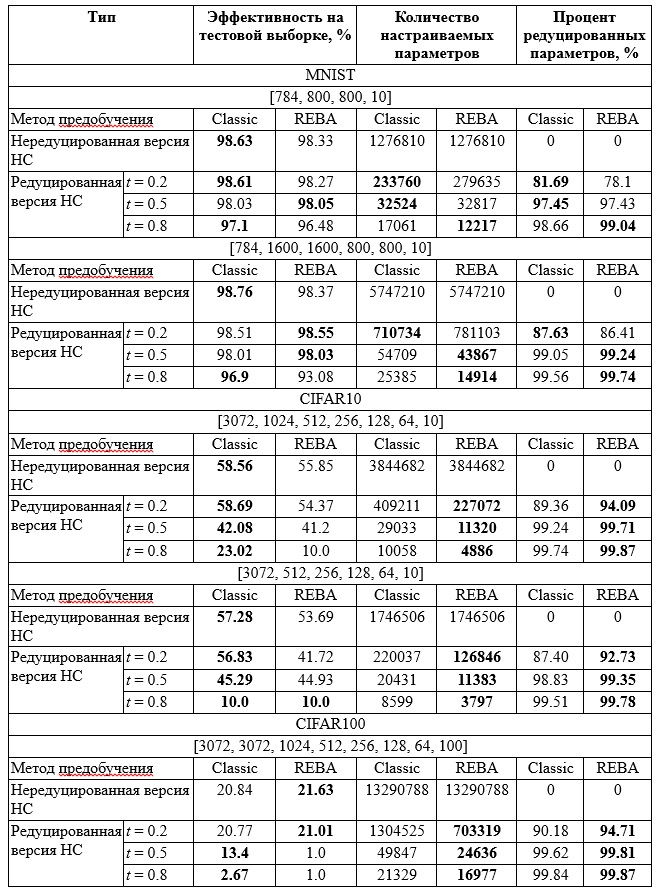
\includegraphics[width=18cm]{man-source/images/ch3/pic3-13.jpg}
% 		\caption{Результаты редуцирования}				
% 		\label{fig:reduce_results}
% 	\end{center}
% \end{figure}

Как видно из приведенных результатов, исследуемые архитектуры в целом сохраняют обобщающую способность, будучи редуцированными более чем на 80 процентов.

Также можно заметить, что чем больше настраиваемых параметров в модели, тем эффективней осуществляется редуцирование. Однако с увеличением параметра редуцирования эффективность исходной сети постепенно снижается, так как редуцированию начинают подвергаться параметры, наличие которых влияет на выходы нейронной сети.

Полученные результаты обосновывают возможность предобучения глубокой нейронной сети с использованием неконтролируемой процедуры без получения эффекта переобучения и снижения эффективности модели, так как в процессе предобучения фактически снижается влияние определенных параметров модели на итоговую выходную активность сети. Такие параметры имеют ``паразитический'' характер и фактически являются фактором переобучения модели. На этапе <<тонкой настройки>> модели они не модифицируются и могут быть удалены после этапа предобучения.
% Продемонстрируем эффективность предложенного подхода на примере редуцирования различных архитектур полносвязных нейронных сетей, применяемых для классификации изображений из выборок MNIST [12], CIFAR10 и CIFAR100 [13]. Данные выборки являются классическими для проверки эффективности моделей машинного обучения.
% Нами были проведены серии экспериментов, включающих различные используемые выборки, архитектуры и варианты предобучения. В рамках одной выборки и архитектуры НС текущая инициализация параметров сохранялась для возможности сравнения эффективности различных вариантов предобучающей процедуры.
% Ниже для рассматриваемых выборок приведены основные параметры, включающие скорость обучения, размер мини-батча, моментный параметр и количество эпох для предобучения и дообучения моделей (табл \ref{table:reduce_training_params}).

% \begin{table} [H]
%   \small
%   \caption{Основные параметры обучения}\label{table:reduce_training_params}
% \begin{tabularx}{\hsize}{| X | X | X |}
%   \hline
%     \multicolumn{2}{|c|}{\textbf{Функции активации}} &
%     \textbf{Сигмодные на все слоях, кроме последнего (линейная)}\\
%     \hline
%     \multirow{4}{*}{Обучение} & Скорость обучения & 0.05-0.1\\
%     \cline{2-3}
%     & Размер мини-батча & 100 \\
%     \cline{2-3}
%     & Моментный параметр & 0.9 \\
%     \cline{2-3}
%     & Количество эпох обучения & 50-100\\
%     \hline
%     \multirow{4}{*}{Предобучение} & Скорость обучения & 0.05-0.2\\
%     \cline{2-3}
%     & Размер мини-батча & 32-100 \\
%     \cline{2-3}
%     & Моментный параметр & [0.5, 0.9] \\
%     \cline{2-3}
%     & Количество эпох обучения & 10\\
%     \hline
% \end{tabularx}
% \end{table}

% В результате вычислительного эксперимента были получены результаты для различных архитектур НС и значений параметра редуцирования t (табл. \ref{fig:reduce_results}).

% \begin{figure}[h]
% 	\begin{center}
% 		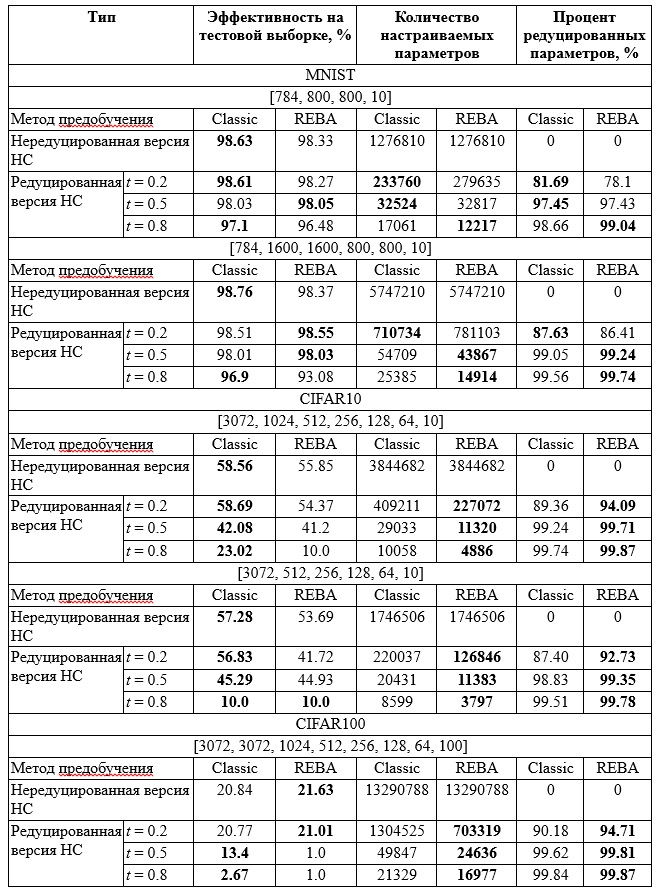
\includegraphics[width=18cm]{man-source/images/ch3/pic3-13.jpg}
% 		\caption{Результаты редуцирования}				
% 		\label{fig:reduce_results}
% 	\end{center}
% \end{figure}
% \begin{table} [H]
%   \small
%   \caption{Результаты редуцирования}\label{table:reduce_results}
% \begin{tabularx}{\hsize}{| X | X | X | X | X | X | X | X |}
%   \hline
%     \multicolumn{2}{|c|}{\textbf{Тип}} & &
%     \multicolumn{2}{|c|}{\textbf{Эффективность на тестовой выборке, \%}} & & \multicolumn{2}{|c|}{\textbf{Количество настраиваемых параметров}} & & \multicolumn{2}{|c|}{\textbf{Процент редуцированных параметров, \%}} &\\
%     \hline
%     \multicolumn{8}{|c|}{MNIST}\\
%     \hline
%     \multicolumn{8}{|c|}{[784, 800, 800, 10]}\\
%     \hline
%     \multicolumn{2}{|c|}{\textbf{Метод предобучения}} & Classic & REBA & Classic & REBA & Classic & REBA\\
%     % \cline{2-3}
%     % & Размер мини-батча & 100 \\
%     % \cline{2-3}
%     % & Моментный параметр & 0.9 \\
%     % \cline{2-3}
%     % & Количество эпох обучения & 50-100\\
%     % \hline
%     % \multirow{4}{}{Предобучение} & Скорость обучения & 0.05-0.2\\
%     % \cline{2-3}
%     % & Размер мини-батча & 32-100 \\
%     % \cline{2-3}
%     % & Моментный параметр & [0.5, 0.9] \\
%     % \cline{2-3}
%     % & Количество эпох обучения & 10\\
%     \hline
% \end{tabularx}
% \end{table}

Помимо редуцирования параметров, было выполнено так называемое архитектурное редуцирование (шаг 3 алгоритма), на котором производилось упрощение структуры слоев моделей за счет исключения нейронов с нулевыми векторами связей.

В следующих таблицах (\ref{table:architect_reduce_mnist_one}, \ref{table:architect_reduce_mnist_two}) приведены результаты архитектурного редуцирования для двух различных архитектур и обучающей выборки MNIST. Для предобучения использовался метод REBA.

\begin{table} [!h]
  \small
  \caption{Результаты для сети 784-800-800-10 на выборке MNIST}\label{table:architect_reduce_mnist_one}
    \centering
    \begin{tabular}{| p{2cm} | p{6cm} | p{6cm} |}
    \hline
        \textbf{Параметр} & \textbf{Исходная} & \textbf{Редуцированная}\\
    \hline
    t=0.2 & 784-800-800-10 & 784-800-556-10\\
    \hline
    t=0.5 & -//- & 784-710-422-10\\
    \hline
    t=0.9 & -//- & 784-91-114-10\\
    \hline
    \end{tabular}
    \end{table}
    
\begin{table} [!h]
  \small
    \caption{Результаты для сети 784-1600-1600-800-800-10 на выборке MNIST}\label{table:architect_reduce_mnist_two}
    \centering
    \begin{tabular}{| p{2cm} | p{6cm} | p{6cm} |}
    \hline
        \textbf{Параметр} & \textbf{Исходная} & \textbf{Редуцированная}\\
    \hline
    t=0.2 & 784-1600-1600-800-800-10 & 784-889-192-686-221-10\\
    \hline
    t=0.5 & -//- & 784-464-157-567-182-10\\
    \hline
    t=0.9 & -//- & 784-17-101-118-50-10\\
    \hline
    \end{tabular}
    \end{table}
    
Из приведенных таблиц можно заметить, что для моделей с большим количеством слоев и нейронов в каждом слое вероятность архитектурного редуцирования выше и оно начинает происходить уже для сравнительно небольших значений параметра редуцирования \textit{t}, в том время как для более <<поверхностных>> моделей оно существеннее проявляется только для больших значений параметра. Стоит отметить, что архитектуры, которые сохраняют почти все нейроны (например, \ref{table:architect_reduce_mnist_one}, архитектура при \textit{t}=0.2), все же при этом теряют для каждого нейрона основную часть связей (сохранение нейрона в данном случае будет иметь место, даже при сохранении одной связи нейрона с предыдущим слоем).

% \textit{Вторая группа} экспериментов проводилась с использованием выборок CIFAR-10 и CIFAR-100 над сверточной архитектурой вида 32 х 3 х 3 -- 32 х 3 х 3 -- 64 х 3 х 3 -- 64 х 3 х 3 -- 128 х 3 х 3 -- 128 х 3 х 3 -- 2048 х 512 -- 512 х \textit{N}, где \textit{N} -- это количество классов (для CIFAR-10 -- 10 классов, для CIFAR-100 -- 100 классов).

% В результате вычислительного эксперимента были получены сравнительные результаты для трех основных вариантов обучения –- без осуществления редуцирования (стандартный режим обучения), с редуцированием по предлагаемому алгоритму и с редуцированием по существующему алгоритму прунинга \cite[c.~1]{wang2019pruning} (таблица \ref{table:cifar_10_conv} и \ref{table:cifar_100_conv}).

% \begin{table} [!h]
%   \small
%   \caption{Результаты для сверточной сети на выборке CIFAR10}\label{table:cifar_10_conv}
% \centering
% \begin{tabular}{| p{3.5cm} | p{4cm} | p{4cm} | p{3cm} |}
%   \hline
%     \textbf{Тип} & \textbf{Эффективность на тестовой выборке, \%} & \textbf{Процент редуцированных параметров по слоям, \%} & \textbf{Средний процент редуцирования, \%}\\
%     \hline
%     Нередуцированная сеть & 71.79 & -- & 0\\
%     \hline
%     Редуцированная сеть (классический прунинг) & 71.63 & 10.76, 9.30, 8.88, 8.01, 8.02, 8.17, 7.97 & 8.73\\
%     \hline
%     Редуцированная сеть (предлагаемый алгоритм) & \textbf{73.47} & 8.45, 8.65, 8.55, 8.24, 7.95, 7.97, 7.97 & 8.25\\
%     \hline
% \end{tabular}
% \end{table}

% \begin{table} [!h]
%   \small
%   \caption{Результаты для сверточной сети на выборке CIFAR100}\label{table:cifar_100_conv}
% \centering
% \begin{tabular}{| p{3.5cm} | p{4cm} | p{4cm} | p{3cm} |}
%   \hline
%     \textbf{Тип} & \textbf{Эффективность на тестовой выборке, \%} & \textbf{Процент редуцированных параметров по слоям, \%} & \textbf{Средний процент редуцирования, \%}\\
%     \hline
%     Нередуцированная сеть & 35.51 & -- & 0\\
%     \hline
%     Редуцированная сеть (классический прунинг) & 34.02 & 10.42, 7.47, 7.92, 8.25, 7.97, 8.00, 7.94 & 8.28\\
%     \hline
%     Редуцированная сеть (предлагаемый алгоритм) & \textbf{40.41} & 9.49, 8.18, 8.12, 7.93, 8.13, 8.05, 7.94 & 8.26\\
%     \hline
% \end{tabular}
% \end{table}

% Во всех экспериментах использовался параметр редуцирования $s=0.1$ (формула \ref{eq:reduction_param}).

% Можно заметить, что предлагаемый алгоритм обладает большей однородностью в выполнении редуцирования по слоям, в то время как классический подход осуществляет более заметное редуцирование первых слоев нейронной сети. Несмотря на то, что получившийся средний процент редуцирования для предлагаемого алгоритма ниже, чем у классического,
% можно отметить, что классический подход уступает предлагаемому в обобщающей способности редуцированной версии.

\section{Выводы}

\begin{easylistNum}
    & Проведен сравнительный анализ методов предобучения ГНС для задачи сжатия данных с использованием автоэнкодерной модели НС [\citen{2-A}, c.~10; \citen{5-A}, c.~14-15; \citen{1-A}, c.~143-145; \citen{20-A}; \citen{21-A}].
    & Проведен сравнительный анализ методов предобучения ГНС для задачи классификации с использованием выборок Iris flower, MNIST, CIFAR-10 и CIFAR-100. Предложена модификация метода предобучения [\citen{2-A}, c.~11; \citen{3-A}, c.~11; \citen{20-A}; \citen{21-A}; \citen{22-A}].
    %& Проведена серия экспериментов по визуализации данных выборки MNIST с применением предлагаемого метода предобучения.
    %& Проведены экспериментальные исследования по решению задачи семантического кодирования изображений из выборки CIFAR-10 с применением глубокой автоассоциативной нейронной сети и предлагаемого метода предобучения.
    & Проведены экспериментальные исследования редуцирования параметров глубокой нейронной сети с использованием различных методов предобучения и архитектур ГНС [\citen{11-A}, c.~298; \citen{30-A}, c.~130-131].
\end{easylistNum}

\chapter{Разработка систем компьютерного зрения на основе глубоких нейронных сетей}

Научные и практические результаты, полученные в рамках данной диссертационной работы, внедрены и используются на следующих предприятиях Республики Беларусь:

\begin{easylist}
     & ОАО <<Савушкин продукт>> (г. Брест) при разработке системы автоматического контроля качества нанесения маркировки продукции;
     & <<Intelligent Semantic Systems>> (г. Минск) при разработке модуля компьютерного зрения для осуществления распознавания лиц пользователей и оценки их эмоционального состояния;
     & в учебном процессе учреждения образования <<Брестский государственный технический университет>>.
 \end{easylist}

Сведения об использовании результатов диссертационной работы отражены в соответствующих актах внедрения, приведенных в приложении \ref{app:b}.

\section{Автоматический контроль качества нанесения маркировки продукции}

\subsection{Постановка задачи и обзор существующих решений}

В основе конкурентности любого производства лежит выпуск разнообразной и качественной продукции. Качество является определяющим критерием при выборе клиентом того или иного продукта, а разнообразие позволяет охватить различные группы потенциальных покупателей. Системы, которые автоматизируют процесс проверки качества и при этом поддерживают многообразие продукции, выпускаемой на большом предприятии, имеют особую ценность. При этом процесс проверки качества осуществляется не только для самого продукта, но и для той упаковки и маркировки, которую видит покупатель. Так как упаковка формирует первоначальное впечатление о товаре, ее качество является одной из причин, которая дает покупателю основание для покупки. Маркировка как элемент упаковки, гарантирует покупателю сохранность продукции в течение указанного срока при соблюдении условий хранения.

В последнее время методы искусственного интеллекта в целом и машинного обучения в частности широко используются в промышленных системах, устанавливаемых на предприятиях для контроля за процессом производства. Интеллектуальные подсистемы позволяют упростить многие рутинные операции, проводимые для поддержания качества готовой продукции. Например, контроль за правильностью нанесения маркировки ранее производился исключительно оператором-человеком. Сейчас, с развитием теории компьютерного зрения, получившей значительный рывок благодаря постоянно развивающейся области обучения глубоких нейронных сетей, становится особенно актуальной разработка систем, позволяющих осуществлять рутинные операции быстрее и регулярнее, чем это мог бы сделать человек.

Поставленная перед нами задача заключалась в разработке системы распознавания маркировки продукции, производимую ОАО <<Савушкин продукт>>. Важным аспектом является то, что распознавание должно выполняться в реальном времени, основываясь на данных, поступающих с камеры, установленной над производственной линией. Результаты производимого распознавания используются для контроля корректности маркировки.

% Помимо буквенно-цифрового кода (рис. \ref{fig:digital_code}), начиная с недавнего времени, продукция может выпускаться с вариантами маркировки, включающей код Data Matrix (рис. \ref{fig:data_matrix}) \cite{milk}. Данный тип маркировки является удобным и емким представлением специальных и общих данных о продукте. 

% \begin{figure}[ht]
% 	\centering
% 	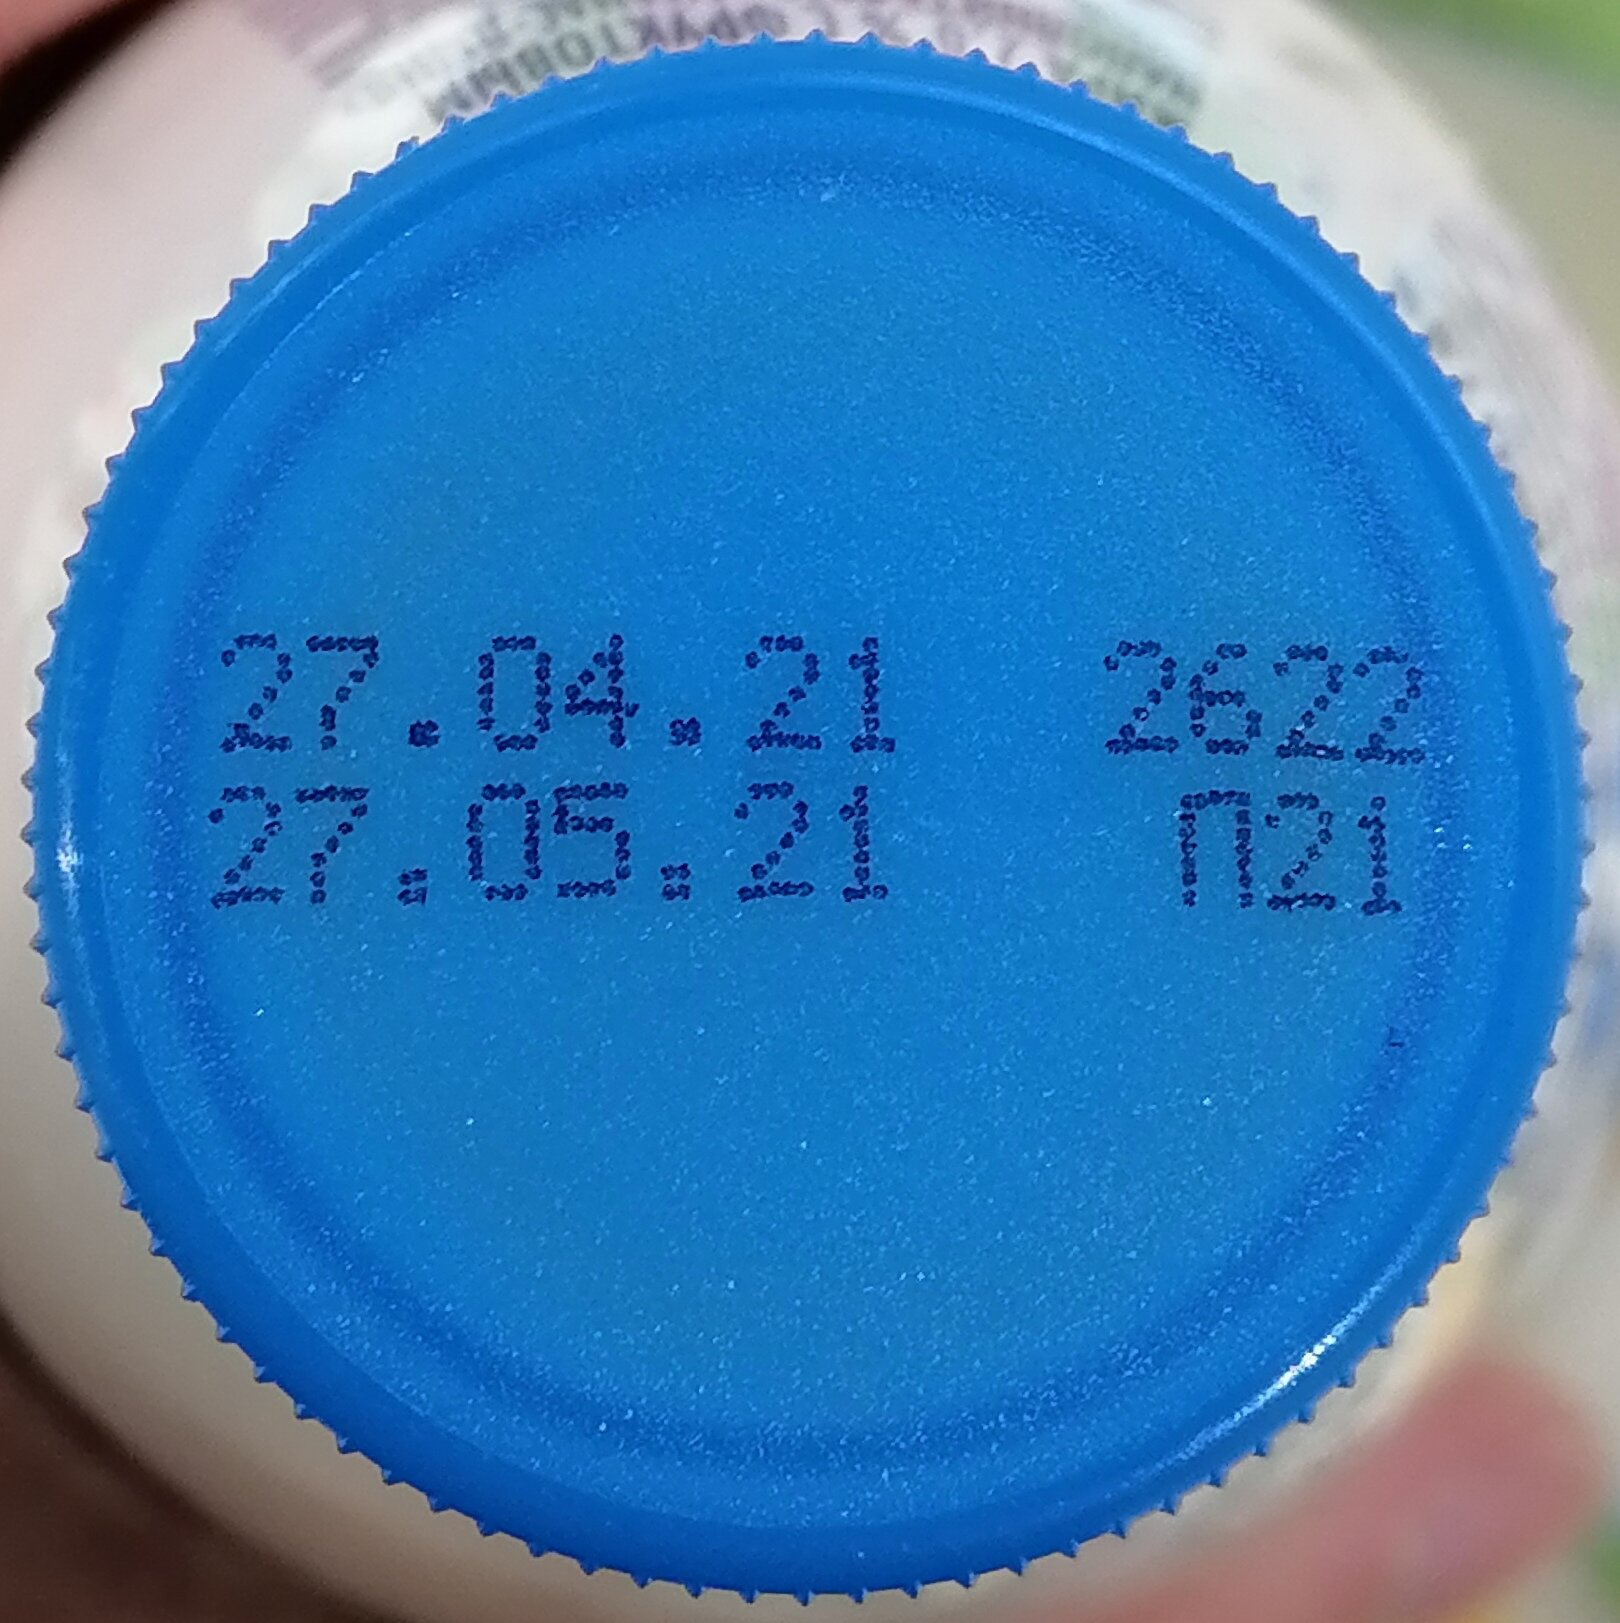
\includegraphics[width=6cm]{man-source/images/ch4/pic4-1.jpg}
% 	\caption{Продукт с буквенно-цифровой маркировкой}
% 	\label{fig:digital_code}
% \end{figure}

% \begin{figure}[ht]
% 	\centering
% 	
\includegraphics[width=10cm]{man-source/images/ch4/pic4-2.jpg}
% 	\caption{Продукт с кодом Data Matrix}
% 	\label{fig:data_matrix}
% \end{figure}

% Основываясь на общей постановке задачи, были выделены следующие подзадачи, которые должна решать система:
% \begin{easylistNum}
%     & обнаружение и распознавание типа маркировки;
%     & распознавание маркировки;
%     & выявление возможных проблем с маркировкой.
% \end{easylistNum}

Перечислим основные возникающие на производстве проблемы с маркировкой \cite{26-A}:

\begin{easylistNum}
    & \textbf{отсутствие чернил:} в случае поступления на конвейер продуктов без маркировки, система должна сделать вывод об отсутствии чернил, опционально запросив проверку, обратившись к принтеру;
    & \textbf{сдвиг камеры:} если от нейросетевых модулей не поступают данные о результатах распознавания, но системе известно, что движение по конвейеру началось, то она должна сделать вывод о сдвиге камеры;
    & \textbf{ошибочная маркировка:} маркировка была обнаружена и распознана, но не совпала с эталонным представлением. В этом случае должен быть сделан вывод о том, что маркировка неверная;
    & \textbf{нечитаемая маркировка:} в случае, если маркировка получается смазанной и не может быть распознана, необходимо остановить конвейер и сообщить об ошибке оператору.
\end{easylistNum}

Для 1,3 и 4 проблемы необходимо выполнить отсев продуктов, которые имеют ``проблемную'' маркировку. Возникновение этих проблем предполагает полную остановку движения конвейера и сообщение оператору о возникшей проблеме.

Следует отметить, что разработанная система является частью более общей системы, управляющая логика которой реализована с использованием технологии OSTIS и используется для анализа указанных проблем маркировки. 
Наша задача заключалась в разработке подсистемы компьютерного зрения для распознавания маркировки продукции.

В процессе решения задачи распознавания маркировки возникают следующие проблемы, влияющие на процесс решения и подбор алгоритмов:

\begin{easylist}
	& \textbf{Высокая скорость видеопотока}. Так как скорость видеопотока составляет 76 кадров в секунду, то время обработка каждого кадра составляет около 13 миллисекунд. Следует отметить, что этого времени недостаточно для запуска сложной нейросетевой архитектуры.
	& \textbf{Невозможность корректной прямой детекции цифр}. Помимо цифр, содержащихся непосредственно в маркировке, в кадр могут попадать цифры, нанесенные на другие объекты, например, на сам конвейер или его части. Помимо этого, следует отметить, что изображение попадает на нейронную сеть с уменьшенным разрешением, что приводит к сложности распознавания очень мелких объектов (цифр).
	& \textbf{Возможность изменения ориентации маркировки}. В процессе движения товара по производственной линии возможен поворот маркировки на произвольный угол, что приводит к существенному ухудшению распознавания.
\end{easylist}

Таким образом, резюмируя все вышеназванные задачи и возникающие проблемы, перечислим основные требования, которым должна удовлетворять разрабатываемая система:

\begin{easylist}
    & \textbf{Высокая скорость работы}. Конвейер движется очень быстро, поэтому распознавание и анализ должны осуществляться с минимальными задержками;
    & \textbf{Автономность}. Система должна минимизировать участие оператора;
    & \textbf{Универсальность}. Система должна настраиваться на распознавание маркировки любой продукции;
    % & \textbf{Адаптируемость}. Система должна работать при любых условиях, возникающих на производстве (например, недостаточность освещения, ошибки персонала и т.д.).
\end{easylist}

%Помимо отслеживания маркировки одного лишь человекочитаемого типа (например, буквенно-цифрового), модульная реализация подобных систем позволяет провести универсализацию процесса распознавания и легко добавлять подготовленные модели, осуществляющие распознавание новых типов маркировок, к которым, например, можно отнести код Data Matrix. Такой особый тип матричных штрих-кодов позволяет закодировать специальную идентификационную информацию, а также вес, срок годности, номер серии, номер партии и дату изготовления продукта \cite{datamatrix}.
%Предлагаемая работа посвящена разработке нейросетевого компонента, являющегося частью более общей нейросимволической системы, описанной в \cite{golovko2020}.
Несмотря на существующий интерес к автономизации производственных процессов и те неоспоримые преимущества, которые влечет ее внедрение, задачи, подобные описанной, решаются в большом числе случаев с участием человека. Оператор просто периодически выборочно проверяет часть продукции. У такого подхода есть недостатки:

\begin{easylist}
    & контроль проходит малая часть продукции, таким образом есть вероятность, что дефектная маркировка будет пропущена;
    & скорость реакции человека на возникающую нештатную ситуацию может быть недостаточной;
    & человек может не заметить небольшое расхождение проверяемой маркировки с эталонной;
    & работа по ручной проверке является монотонной.
\end{easylist}

Существующие разработки базируются на аппаратных решениях, например, на использовании специальных датчиков \cite{omron}.

Такие решения осуществляют распознавание маркировки, но имеют ряд важных недостатков:

\begin{easylist}
	& Нестабильное качество распознавания, зависящее от условий, при которых производится съемка (в частности, от освещенности). Так как производственная линия движется быстро, то необходимые условия для качественного распознавания чаще всего не соблюдаются;
	& Необходимость покупки специализированного программного обеспечения для настройки датчиков.
\end{easylist}

Таким образом, подобные решения создают дополнительные сложности при эксплуатации, которые проявляются в необходимости помимо выборочного ручного контроля качества продукции осуществлять также контроль за функционированием самой системы распознавания.  

\subsection{Предлагаемый подход}

Предлагаемый подход состоит в использовании конвейерной структуры из отдельных нейросетевых модулей, каждый из которых решает собственную подзадачу распознавания маркировки.

Задачей данного данного конвейера является обнаружение маркировки, определение ее типа и ее распознавание.

Остановимся далее подробнее на архитектуре системы.

Осуществляя декомпозицию решаемой задачи можно выделить следующие подзадачи:

\begin{easylistNum}
	& Оценка положения товара;
	& Детекция товара и маркировки;
	& Определение типа маркировки;
	& Поворот маркировки для горизонтальной ориентации;
	& Распознавание маркировки (осуществляется по-разному, в зависимости от типа);
	& <<Сборка>> маркировки: формирование выходной информации (даты производства товара, номера в партии и т.д.);
	& Проверка распознанной маркировки (определение корректности распознанных данных в соответствии с заранее заданным шаблоном).
\end{easylistNum}

Применение предпоследнего этапа в большей степени относится к одному из типов маркировки -- алфавитно-цифровому.

Помимо указанных, в процессе распознавания маркировки решаются дополнительные задачи, связанные с корректностью нанесения такой маркировки.

\begin{easylistNum}
    & определение отсутствия маркировки на продукте;
    & определение наличия искажений маркировки, возникающих в процессе печати, отсутствия ее частей и т.д.
\end{easylistNum}

Указанные задачи решаются в процессе выполнения основных этапов распознавания.

Проблемы, указанные в постановке задачи, могут быть решены архитектурно.

\begin{easylistNum}
    & Высокая скорость видеопотока: решается пропуском незначащих кадров, в которых товар находится не в середине кадра. Это позволяет увеличить интервал времени, необходимый для обработки изображения нейросетью. Таким образом, необходимо оценить значимость кадра. Это можно сделать более простой моделью с малым временем обработки;
    & Невозможность корректной прямой детекции цифр: решается осуществлением декомпозиции задачи обнаружения на отдельные подзадачи. Например, в начале обнаруживается товар, затем маркировка на товаре и, наконец, отдельные цифры;
    & Возможность изменения ориентации маркировки: решается оценкой угла поворота маркировки для представления ее в максимально горизонтальном положении.
\end{easylistNum}

Наличие нескольких подзадач предполагает использование группы моделей, каждая из которых выполняет свою часть работы. 

Следует отметить, что в предлагаемой нейросетевой системе практически для каждой подзадачи используется собственная нейросетевая модель. Это позволяет легко модифицировать систему, улучшать отдельные модули, изменять их, а также добавлять новые. 

Архитектура готового модуля распознавания представлена на рис. \ref{fig:structure}.

\begin{figure}[ht]
	\centering
	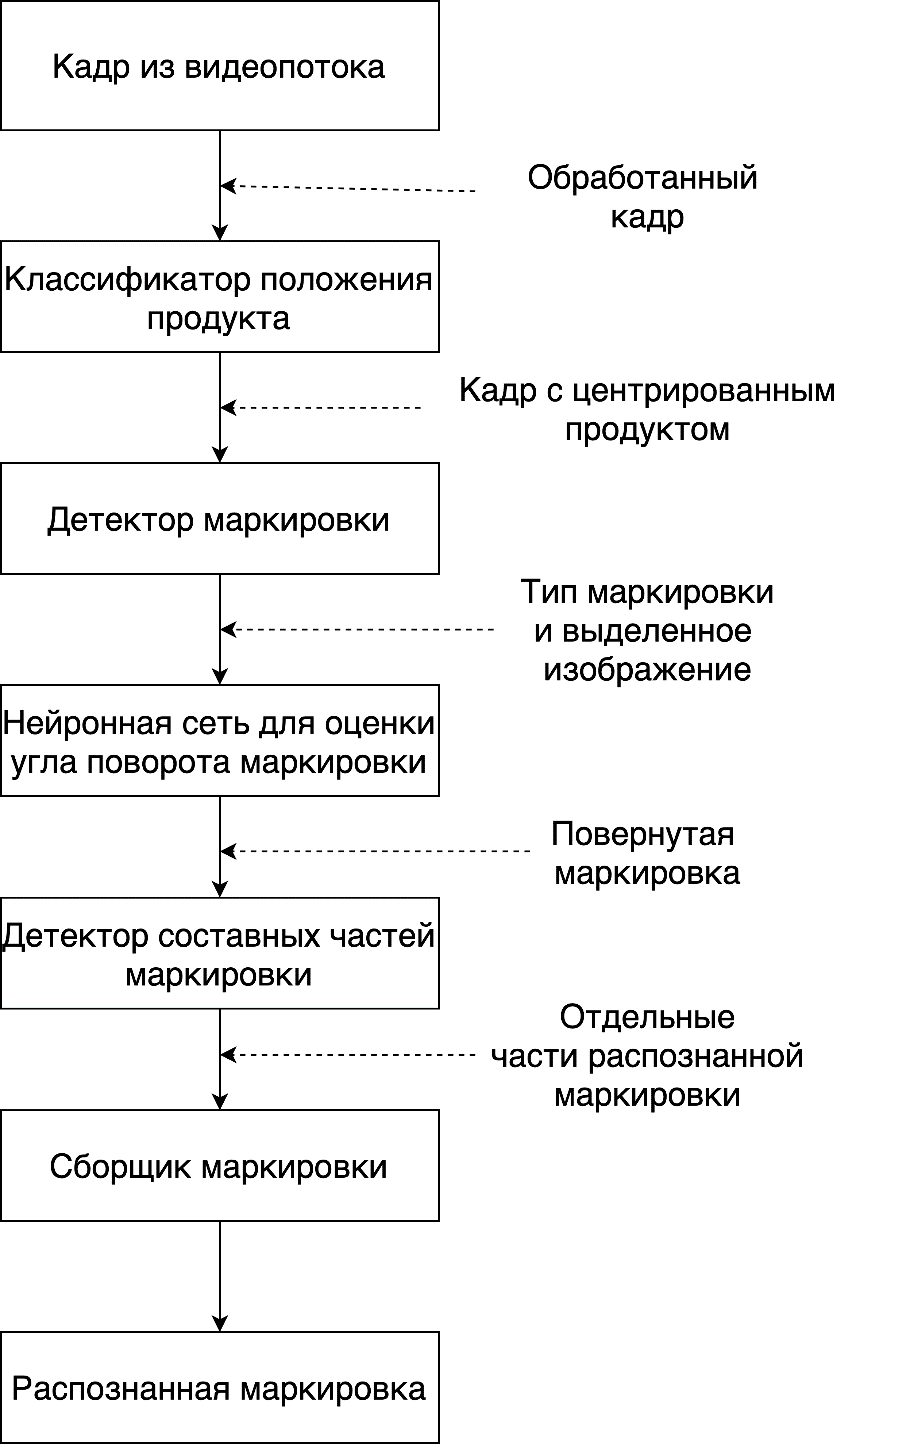
\includegraphics[width=10cm]{man-source/images/ch4/pic4-13.png}
	\caption{Структура модуля распознавания маркировки}
	\label{fig:structure}
\end{figure}

Опишем основные применяемые модули и их роль в общей архитектуре.

\textbf{Классификатор положения продукта.} Первая модуль реализован на основе сверточного классификатора, который определяет значимость кадра для последующего анализа. При этом наиболее значимым является кадр, в котором товар находится ближе всего к центру кадра (рис. \ref{fig:distance_classes}). Было определено четыре основных класса позиций, по мере удаленности продукта от центра кадра. 1 класс описывает минимальную удаленность. Только кадры этого класса участвуют в последующих этапах обработки и анализа. Классы 2 и 3 описывают среднюю и максимальную удаленность. Класс 4 используется для случая отсутствия продукта в кадре (пустая линия).

\begin{figure}[ht]
	\centering
	\includegraphics[width=16cm]{man-source/images/ch4/pic4-24.jpeg}
	\caption{Примеры изображений разных классов по степени удаленности объекта от центра кадра}
	\label{fig:distance_classes}
\end{figure}

Архитектура применяемого классификатора представлена на рис. \ref{fig:nn_class1}. Он состоит из 5 слоев и имеет 4 выходных нейрона по числу классов, определяющих положение товара в кадре. На всех слоях используется функция активации ReLU за исключением 3-го и последнего слоев. Они используют линейную и softmax-функции активации соответственно. Также применяется max pooling после первого и второго сверточного слоев с параметром stride, равным 2.

\begin{figure}[ht]
	\centering
	\includegraphics[width=16cm]{man-source/images/ch4/pic4-4.pdf}
	\caption{Структура классификатора для оценки положения бутылки \cite{26-A}}
	\label{fig:nn_class1}
\end{figure}

В случае, если кадр был отнесен к классу 1, он передается далее на следующую модель. 

\textbf{Модуль детекции маркировки.} В составе данного модуля используется нейросетевой детектор, осуществляющий поиск товара и маркировки в кадре. Здесь в качестве архитектуры была выбрана сеть SSD \cite{liu} на базе классификатора MobileNet v1 \cite{howard}.

Независимое обнаружение товара и маркировки позволяет идентифицировать ситуацию с отсутствующей маркировкой автоматически. Для этого достаточно проверить логическое условие отсутствия маркировки при наличии самого товара в кадре. При выявлении дефекта, система оповещает об этом оператора.

Следует отметить, что данный детектор применяется для обнаружения разных типов маркировки. Так как модель SSD может использоваться для обнаружения объектов разных классов, было принято решение использовать ее и для определения типа маркировок, которое не требует каких-либо специальных процедур анализа. 

В итоге, если дефект маркировки не был обнаружен, выполняется передача изображения маркировки (в оригинальном размере) и информации о ее типе на следующую модель.

\textbf{Модуль оценки угла поворота.} В реализации третьего модуля используется регрессор, применяемый для оценки угла поворота маркировки. Данная модель возвращает угол, на который должна быть повернута маркировка для достижения горизонтальной ориентации изображения. Такое преобразование позволяет улучшить качество последующего распознавания цифр. После поворота выполняется передача изображения маркировки на модель для анализа соответствующего типа маркировки (в нашей реализации это модели для анализа кода Data Matrix или цифровой метки).

\textbf{Детектор составных частей.} Для анализа цифрового кода также используется детектор SSD-MobileNet v1, который обнаруживает отдельные цифры в маркировке.
Для анализа кода Data Matrix в текущей реализации используется не нейросетевая модель. Применимость нейронной сети для подобного анализа может быть предметом дальнейших исследований.  

Далее осуществляется <<сборка>> распознанной маркировки и обработка результата.

Принцип работы нейросетевого компонента на примере буквенно-цифровой маркировки продемонстрирован на рис. \ref{fig:system_work}.

\begin{figure}[!ht]
	\centering
	\includegraphics[width=7cm]{man-source/images/ch4/pic4-5.png}
	\caption{Принцип работы системы}
	\label{fig:system_work}
\end{figure}

\subsection{Обучающие выборки: формирование и основные характеристики}

В процессе подготовки нейросетевых моделей нами использовались различные обучающие выборки:

\begin{easylist}
	& Выборка для обучения классификатора
	& Выборка для обучения детектора маркировок и товаров (определения типа маркировки)
	& Выборка для обучения регрессора угла поворота
	& Выборка для обучения детектора цифр
\end{easylist} 

\textbf{Выборка для обучения классификатора}. Для создания выборки использовалась модель Faster R-CNN \cite{ren} (на базе  предобученного классификатора ResNet50 \cite{he}). Данная модель обладает лучшими показателями эффективности, чем SSD-MobileNet, но уступает ей в скорости. Она использовалась для автоматической разметки имеющихся данных (главным образом видеофайлов производственного процесса) по степени удаленности товара от центра кадра. В качестве метрики применялось эвклидово расстояние от центра продукта до центра кадра. Таким образом были сформированы четыре класса изображений, которые использовались для последующего обучения сверточного классификатора. Общий объем выборки составил 6189 изображений, 1303 из которых составили контрольную выборку.

\textbf{Выборка для обучения детектора маркировок и товаров (определения типа маркировки)}. Для формирования этой выборки мы использовали размеченные вручную изображения из выборки для обучения классификатора и дополнительные изображения сгенерированных кодов Data Matrix. Общий объем выборки составил 815 изображений, 163 из которых составили контрольную выборку.

\textbf{Выборка для обучения регрессора угла поворота}. При создании данной выборки использовались изображения маркировок, повернутые под произвольными углами. Общий объем выборки составил 59385 изображений, 11877 из которых составили контрольную выборку. В качестве основы брались изображения маркировок, полученные из выборки для обучения детектора маркировок и товаров.

\textbf{Выборка для обучения детектора цифр}. Для создания этой выборки применялся датасет номеров домов SVHN \cite{netzer}, а также размеченные цифровые маркировки. Использовался вариант выборки SVHN, включающий 33402 изображения в обучающей части и 13068 в контрольной (рис. \ref{fig:svhn_dataset}). Объем выборки размеченных цифровых маркировок составил 419 изображений.

\begin{figure}[ht]
	\centering
	\includegraphics[width=7cm]{man-source/images/ch4/pic4-14.png}
	\caption{Пример изображений из выборки SVHN}
	\label{fig:svhn_dataset}
\end{figure}

\subsection{Результаты обучения и тестирования} 
После обучения классификатора 1 итоговая точность распознавания составила \textbf{93.27\%}.

Оба детектора (продуктов/маркировок и отдельных цифр) обучались на основе предобученных моделей (использовалось предобучение II типа).

Применение SSD-модели позволяет достичь эффективности детекции в \textbf{99\% (mAP = 0.99)} для обнаружения товара и маркировки и \textbf{92\% (mAP = 0.92)} для отдельных цифр. Кроме этого, скорость обработки позволяет успешно обнаруживать маркировку в видеопотоке со скоростью 76 кадров в секунду. Результаты эффективности распознавания отдельных цифр представлены в таблице \ref{tab:efficiency_detector1}.  

\begin{table}[h]
\caption{Эффективность обнаружения отдельных классов цифр}
\centering
\begin{tabular}{ | c | c |  }
\hline
Class label & AP \\ \hline
0 & 0.9218\\
1. & 0.9107\\
2. & 0.9354\\
3. & 0.9286\\
4. & 0.9265\\
5. & 0.9137\\
6. & 0.9274\\
7. & 0.9167\\
8. & 0.9646\\
9. & 0.8975\\
\hline
\textbf{mAP} & \textbf{0.92429}\\
\hline
\end{tabular}
\label{tab:efficiency_detector1}
\end{table}

Результаты обнаружения детектора маркировок и детектора отдельных цифр изображены на рис. \ref{fig:product_detect}  и \ref{fig:numbers_detect}.

\begin{figure}[!ht]
	\centering
	\includegraphics[width=10cm]{man-source/images/ch4/pic4-25.png}
	\caption{Обнаруженный продукт и маркировка}
	\label{fig:product_detect}
\end{figure}

\begin{figure}[!ht]
	\centering
	\includegraphics[width=12cm]{man-source/images/ch4/pic4-26.png}
	\caption{Обнаруженные цифры в маркировке}
	\label{fig:numbers_detect}
\end{figure}


% \subsection{Заключение}
% В данной работе рассматривается разработка интеллектуального компонента для распознавания маркировки продукции, базирующейся на нейросетевом подходе. Достоинством предложенного решения является использование модульной структуры нейросетевой части, позволяющее осуществлять простую коммутацию между отдельными моделями. Следует отметить универсальность предложенного подхода, которая проявляется в простоте выполнения работы по распознаванию произвольной маркировки на разнообразной продукции. Достаточно интегрировать новый модуль с необходимой функциональностью и система начнет его использовать. Применяемые нами модели отличаются производительностью, благодаря чему возможна работа системы на быстро движущейся производственной линии.

% Направлением дальнейшей работы может быть выбрано улучшение имеющихся результатов распознавания цифровых маркировок, а также исследование применения нейросетевого подхода для распознавания QR-кода.

\section{Обнаружение солнечных панелей на аэрофотоснимках}

\subsection{Постановка задачи и обзор существующих решений}
По причине увеличивающейся доли использования солнечной энергии, спрос на фотоэлектрические элементы в мире постоянно растет. С начала 2010-х годов индустрия производства и поддержки солнечных панелей переживает стремительный рост. Так, по состоянию на 2021 год только в США в данной отрасли работает более 10000 компаний \cite{seia}.

В связи с растущей популярностью этой технологии проблемы, связанные с обслуживанием солнечных панелей, также становятся актуальными. Многие сервисные компании заинтересованы в получении информации о потенциальных клиентах. Таким образом, анализ фотоснимков с целью обнаружения солнечных панелей и накопления статистической информации является актуальной задачей.

%Развитие теории обучения глубоких нейронных сетей [4] дало мощный импульс для разработки различных вариантов сверточных нейронных сетей, применяемых для решения задач распознавания и классификации. Появление технологии параллелизации вычислений с использованием GPU в свою очередь сделало такое обучение осуществимым за приемлемый отрезок времени.

Нами решались задача обнаружения солнечных панелей на изображении с получением точных координат местонахождения с использованием глубоких сверточных нейронных сетей.

Сверточные нейронные сети базируются на моделях неокогнитрона, предложенной К. Фукусимой \cite{fukushima1980}, и сетях с разделяемыми весами. Первая классическая модель сверточной нейронной сети была разработана ЛеКуном и получила название LeNet-5 \cite{lekun1998}. Сверточные нейросети интегрировали три концепции, называемые локальным рецептивным полем, разделяемыми весовыми коэффициентами и пространственной подвыборкой. Используя локальное рецептивное поле, нейронные элементы первого сверточного слоя могут извлекать простейшие признаки, такие как края, углы и т.д. Сверточная нейронная сеть представляет собой комбинацию сверточных и подвыборочных (pooling) слоев (рис. \ref{fig:cnn_common_view}), благодаря чему осуществляет нелинейное иерархическое преобразование входной информации. Последний блок сверточной сети представляет собой многослойный персептрон, SVM или любой другой классификатор.

\begin{figure}[ht]
	\centering
	\includegraphics[width=10cm]{man-source/images/ch4/pic4-15.png}
	\caption{Общий вид сверточной нейронной сети}
	\label{fig:cnn_common_view}
\end{figure}

В статье Дж. Малофа \cite{malof2015} был описан подход, базирующийся на использовании SVM для автоматического обнаружения солнечных панелей, используя фотографии высокого разрешения, полученные с помощью спутника. В этом подходе сначала применяется операция предварительного скрининга, которая идентифицирует регионы, которые затем обрабатываются с целью выделения признаков. В качестве выходной информации, получаемой с помощью данной модели, выступает список регионов и доверительные значения, показывающие, насколько вероятно наличие солнечной панели в заданной области. Общая эффективность подхода определения наличия панелей в \cite{malof2015} составляет порядка 94\%. Однако, нужно отметить, что данный метод дает лишь приблизительную информацию о местонахождении панели. Оценки точности локализации панелей в работе не приводится.

В \cite{malof2016} используется подход, базирующийся на применении деревьев решений. Достигнутый показатель локализации панелей составил 90\% в случае использования определенных параметров алгоритма, а сам метод состоит из четырех стадий. В работе в качестве обучающей выборки используется Aerial Imagery Dataset, включающий изображения разрешением до 5000 Х 5000 пикселей \cite{bradbury2016}.

\subsection{Предлагаемый подход}

Предложенный нами нейросетевой алгоритм для обнаружения солнечных панелей отличается тем, что в качестве базовой модели используется сверточная нейронная сеть, которая показывает лучшие результаты при решении задач классификации и детекции объектов на изображениях. Другое важное отличие заключается в использовании фотографий низкого разрешения для обучения нашей модели (например, фото из Google Maps, нередко неудовлетворительного качества, см. рис. \ref{fig:example_of_images}). 

\begin{figure}[ht]
	\centering
	\includegraphics[width=16cm]{man-source/images/ch4/pic4-16.png}
	\caption{Примеры изображений низкого качества из обучающей выборки}
	\label{fig:example_of_images}
\end{figure}

Предлагаемый алгоритм обнаружения панелей включает два основных этапа, на каждом из которых используется предобученная глубокая нейронная сеть: 

\begin{easylistNum}
    & Оценка наличия солнечной панели на аэрофотоснимке
    & Локализация солнечной панели
\end{easylistNum}

Использование двухэтапности в решении поставленной задачи позволяет существенно ускорить обработку изображений, большую часть которых занимают объекты, отличные от искомых (солнечных панелей), т.к. нейросетевые модели, используемые на этапе локализации, как правило, более ресурсоемки. Таким образом, модель первого этапа выполняет роль фильтра для последующей обработки. Тем самым предлагаемый алгоритм можно применять для последовательной обработки больших изображений.

\textbf{Оценка наличия солнечной панели}. Для первого этапа в качестве базовой модели для решения поставленной задачи мы использовали сверточную нейронную сеть с архитектурой, представленной на рис. \ref{fig:used_cnn} [35]. 

Представленная нейронная сеть состоит из шести слоев. Первые три слоя являются сверточными и выполняют выделение высокоуровневых признаков. Последние три слоя представляют собой полносвязные слои нейронных элементов, решающие задачу классификации. Для всех слоев, кроме последнего, используется функция активации ReLU \ref{eq:relu_function}.

\begin{figure}[ht]
	\centering
	\includegraphics[width=17cm]{man-source/images/ch4/pic4-19.jpg}
	\caption{Архитектура используемой сверточной нейронной сети}
	\label{fig:used_cnn}
\end{figure}

\begin{equation}
    \label{eq:relu_function}
    f(x) = max(0, x)
\end{equation}

В последнем полносвязном слое используется сигмоидная функция активации \ref{eq:sigmoid_function}.

\begin{equation}
    \label{eq:sigmoid_function}
    f(x) = \frac{1}{1+e^{-x}}
\end{equation}

Дополнительно, на первом сверточном слое мы используем шаг, равный 3, с целью уменьшения размерности получаемых со сверточного слоя карт признаков.

Изображения из обучающей выборки подавались на первый слой сверточной сети и передавались вплоть до последнего слоя. Последний полносвязный слой содержит только один нейрон, который возвращает вероятность наличия солнечной панели на изображении. Для обучения сверточной нейронной сети использовался метод стохастического градиентного спуска. 

\textbf{Локализация солнечной панели}. Для решения задачи локализации нами применялась глубокая нейронная сеть Faster-RCNN (Faster Region-based Convolutional Neural Network), базирующаяся на классификаторе ResNet-50 (\ref{fig:faster_rcnn}). Данная модель состоит из двух частей. Первая часть -- это классификатор ResNet-50, предобученный на выборке COCO \cite{lin2015}. Вторая часть -- это детектор, который представлен сверточной нейронной сетью, генерирующей координаты прямоугольных областей, содержащих в себе искомые объекты, и метки класса для каждой такой области.

\begin{figure}[ht]
	\centering
	\includegraphics[width=17cm]{man-source/images/ch4/pic4-21.jpg}
	\caption{Глубокая сверточная сеть Faster-RCNN}
	\label{fig:faster_rcnn}
\end{figure}

Подобная архитектура обеспечивает получение высоких показателей эффективности при решении задач детекции объектов в системах, где общее время, затраченное на обработку и вывод результатов, некритично.

\subsection{Обучающая выборка}
В качестве исходных данных, используемых для формирования обучающей выборки для решения задачи обнаружения солнечных панелей, нами использовались цветные изображения Google Maps с разрешением 200 Х 200 пикселей (рис. \ref{fig:google_maps}).

\begin{figure}[ht]
	\centering
	\includegraphics[width=12cm]{man-source/images/ch4/pic4-17.png}
	\caption{Примеры изображений из выборки Google Maps}
	\label{fig:google_maps}
\end{figure}

Для обучения модели первого этапа использовалась выборка из 3347 фотографий (где 1643 изображения содержали солнечные панели, а 1704 -- не содержали), при этом 80\% исходной выборки формировали обучающую выборку, а 20\% - тестовую. Для обучения модели второго этапа использовалась выборка из 1000 изображений, 800 из которых было отнесено к обучающей, а 200 -- к тестовой выборкам.

Подготовка обучающей выборки состояла в ручном переборе изображений и отнесении их к двум группам изображений -- содержащих солнечные панели и, соответственно, не содержащих. При подготовке выборки для локализации панелей также использовался ручной перебор изображений с определением для каждого характеристик прямоугольных областей, включающих солнечные панели (длина, ширина, координаты левого верхнего угла). Интересующих областей на изображении может быть несколько (для случая множественных панелей). 

Выделение прямоугольных областей для некоторых изображений может не выглядеть целесообразным, например, случаи, когда панели расположены под углом к горизонтальной оси снимка и имеют вытянутую форму (рис. \ref{fig:background_dominate}). Однако, для таких фотографий удается получить приемлемые результаты локализации на тестовых данных, несмотря на то, что большая часть области включает фоновое изображение.
 
\begin{figure}[ht]
	\centering
	\includegraphics[width=8cm]{man-source/images/ch4/pic4-18.png}
	\caption{Пример изображения с преобладающим фоном}
	\label{fig:background_dominate}
\end{figure}

\subsection{Оценка качества обученных моделей}

Для оценки качества применялись две основные метрики. 

Первая метрика использовалась для оценки классификатора. В режиме тестирования модели нами применялось простое преобразование выходных данных -- пороговая функция вида:

\begin{equation*}
    b_s = I[y_s > 0,5]
\end{equation*}
где $y_s$ представляет реальное выходное значение CNN-сети, возвращаемое для $s$-го входного изображения выборки, $b_s$ -- бинаризованная форма, полученная вычислением индикаторной функции вида:

\begin{equation*}
    I[x] = 
    \begin{cases}
        1, & \text{x is True} \\
        0, & \text{x is False}
    \end{cases}
\end{equation*}

Метрика оценки рассчитывалась по формулам:

\begin{equation*}
    A = \frac{S}{L} * 100\%
\end{equation*}

\begin{equation*}
    S = \sum_{s=1}^L I[b_s = e_s]
\end{equation*}
где $e_s$ -- эталонное значение (метка), $L$ -- объем выборки. Таким образом, оценивается доля верных ответов, возвращаемых нейронной сетью.

Для оценки эффективности модели локализации использовалась метрика mAP.

Метрика mAP является стандартом де-факто метрик, используемых для оценки качества моделей, применяемых для детекции. Эта метрика используется вместе со своими модификацими, вычисленными для различных значений порога IoU. Так как для рассматриваемой задачи существует только один класс объектов, метрика mAP совпадает с AP.

Как известно, точность вычисляется по формуле:

\begin{equation*}
    P = \frac{TP}{TP + FP}
\end{equation*}
где \textit{TP} и \textit{FP} обозначают соответственно число истинно-положительных и ложно-положительных результатов детекции, и, соответственно, \textit{P} определяет долю корректных детекций в общем числе детекций, полученных моделью.

Значение \textit{TP} определяет общее количество прямоугольных областей, для которых величина \textit{IoU}, вычисленная относительно истинных областей (\textit{Ground-true box}), больше некоторого заданного порога (чаще всего выбирается порог 0,5). Таким образом, если величина \textit{IoU} для такой спрогнозированной области превысила 0,5, то детекция рассматривается как истинно-положительная. Если детекций для данной истинной области несколько, то выбирается одна детекция с самым большим значением \textit{IoU}, а остальные рассматриваются как \textit{FP}.

Усредненное значение по всем изображениям выборки дает величину AP:

\begin{equation*}
    AP = \frac{1}{L} \sum_{i=1}^L \frac{TP_i}{TP_i + FP_i}
\end{equation*}
где \textit{L} -- число изображений в выборке.

\subsection{Результаты обучения и тестирования}

Сверточная сеть для определения наличия солнечных панелей обучалась в течение 70 эпох, используя следующие параметры:

\begin{easylist}
    & скорость обучения -- 0,001;
    & моментный параметр -- 0,9;
    & weight-decay -- 0,0005;
    & размер мини-батча -- 20.
    & вероятность применения dropout для полносвязных слоев -- 0,5
\end{easylist}

Точность классификации для данной задачи, составила порядка \textbf{87,46\%} (см. таблица \ref{table:confusion_matrix}).

\begin{table} [H]
  \small
  \caption{Матрица ошибок}\label{table:confusion_matrix}
\begin{tabularx}{\hsize}{| X | X | X | X |}
  \hline
    & Спрогнозировано <<No>> & Спрогнозировано <<Yes>> & Точность,\% \\
    %\cline{2-3}
    \hline
    Ожидалось <<No>> & 325	& 32	& 91\\
    \hline
    Ожидалось <<Yes>>	& 52	& 261	& 83\\
    \hline
    Итого & 377	& 293	& 87\\
    \hline
\end{tabularx}
\end{table}

На рис. \ref{fig:roc_curve} изображена ROC-кривая, построенная для обученного классификатора.

\begin{figure}[ht]
	\centering
	\includegraphics[width=11cm]{man-source/images/ch4/pic4-20.jpg}
	\caption{ROC-кривая для обученного бинарного классификатора, AUC = 0,92}
	\label{fig:roc_curve}
\end{figure}

Другие характеристики полученного классификатора: 
\begin{easylist}
    & полнота = 0,8339, 
    & специфичность = 0,9104, 
    & точность = 0,8907, 
    & F-мера = 0,8614.
\end{easylist}

Сеть для локализации объектов обучалась в течение 5000 итераций (под итерацией здесь понимается настройка параметров для одного случайного изображения из обучающей выборки), используя следующие параметры:

\begin{easylist}
    & скорость обучения -- 0,0003;
    & моментный параметр -- 0,9;
\end{easylist}

После выполнения обучения, нами проводилось исследование обобщающей способности сети с использованием тестовой выборки из 200 изображений. Полученный результат составил \textbf{\textit{AP}=0,9299}.

На рис. \ref{fig:test_results} изображены некоторые результаты детекции солнечных панелей на изображениях низкого разрешения.

\begin{figure}[ht]
	\centering
	\includegraphics[width=16cm]{man-source/images/ch4/pic4-22.png}
	\caption{Результаты детекции для изображений из тестовой выборки}
	\label{fig:test_results}
\end{figure}

Как можно видеть, предложенный метод осуществляет достаточно точное обнаружение. На рис. \ref{fig:random_results} изображены результаты работы метода для произвольных изображений (не из тестовой выборки).

\begin{figure}[ht]
	\centering
	\includegraphics[width=16cm]{man-source/images/ch4/pic4-23.png}
	\caption{Результаты детекции для произвольных изображений}
	\label{fig:random_results}
\end{figure}

% \section{Обнаружение и распознавание лиц с функцией дообучения}

%\subsection{Постановка задачи}

%\subsection{Предлагаемый подход}

% Рассмотрим подробнее архитектуру системы компьютерного зрения и принцип действия семантического анализатора. 

% \subsection{Структура модуля компьютерного зрения}

%Модуль компьютерного зрения состоит из последовательности связанных между собой нейросетевых и вспомогательных модулей, используемых для решения задач, которые образуют своеобразный конвейер. %pipeline  

%Связи между этими модулями могут быть организованны как последовательно, так и параллельно. Нейросетевые модули используют нейросетевую модель для решения задачи распознавания, а также выполняют преобразования входных данных модуля во входные данные модели. Вспомогательные модули не используют нейросетевые модели и нужны для преобразования входных данных, выполняемого однократно для нескольких нейросетевых модулей.

%На этапе проектирования конвейера нужно ответить на вопросы, выполняются ли модули параллельно и являются ли выходные данные одного модуля входными данными для другого. Таким образом возникают две топологии -- одна описывает связь модулей с точки зрения параллельности их работы, другая -- с точки зрения передачи входных данных.

%На вход конвейера подается видео-поток, который с помощью вспомогательных модулей разбивается либо на кадры, либо на видеофрагменты. Полученные выходные данные подаются на вход соответствующим веткам конвейера.

%Предложенная модель (\ref{fig:common_arch}) с независимо подключаемыми нейросетевыми модулями позволяет осуществлять параллелизацию вычислений и тем самым уменьшать общее время, затрачиваемое на обработку входных данных. Использование вспомогательных модулей и гибкой настройки связей по входам и выходам позволяет избежать повторной обработки входных данных для различных нейросетевых модулей. 

% Структура разработанного модуля компьютерного зрения представлена на рис. \ref{fig:general_diagram}. Схема сильно упрощена с точки зрения взаимодействия с базой знаний и отражает только последовательность и связанность модулей компьютерного зрения. Рассмотрим данные модули более подробно.

% \begin{figure}[ht]
% 	\centering
% 	\includegraphics[width=8cm]{man-source/images/ch4/pic4-8.png}
% 	\caption{Конвейер нейросетевых моделей для распознавания маркировки}
% 	\label{fig:general_diagram}
% \end{figure}

% \textbf{Модуль детекции лица} решает задачу обнаружения лиц в кадре. Принимает на вход кадр из видеопотока и возвращает координаты найденных лиц.

% \textbf{Модуль идентификации} нужен для распознавания лица идентифицируемого пользователя. Принимая на вход координаты обнаруженных лиц, данный модуль возвращает идентификаторы пользователей.

% \textbf{Модуль распознавания эмоций} является независимым от логики идентификации. Как и модуль идентификации, принимает на вход координаты обнаруженных лиц и возвращает вероятностный вектор эмоций. 

% После выполнения отдельных веток конвейера, результаты работы модулей передаются на вход интегратора, который выполняет погружение в базу знаний.

% Далее рассмотрим подробнее основные функции модуля компьютерного зрения и полученные результаты при подготовке соответствующих нейросетевых моделей.

% \subsection{Функции модуля компьютерного зрения}

% К функция модуля компьютерного зрения относятся:
% \begin{easylist}
%     & идентификация известного системе пользователя;
%     & идентификация неизвестных пользователей после дообучения; 
%     & распознавание эмоций пользователей.
% \end{easylist}

% \textbf{Идентификация пользователя}. Идентификация пользователя осуществляется модулем идентификации. Наиболее полно процессы, происходящие в модуле, представлены в блок-схеме на рис. \ref{fig:id_flowchart}.

% \begin{figure}[ht]
% 	\centering
% 	\includegraphics[width=8cm]{man-source/images/ch4/pic4-9.jpg}
% % 	\caption{The overall flowchart of identification}
% 	\caption{Общая блок-схема идентификации}
% 	\label{fig:id_flowchart}
% \end{figure}

% Для реализации данной функции применяется модель нейронной сети FaceNet \cite{facenet}. Для данной модели используются классические модели глубоких сверточных нейронных сетей с триплет-функцией потерь. В нашем случае использовалась сверточная сеть ResNet \cite{resnet}. Общая схема модели представлена на рис. \ref{fig:FaceNet}. 

% \begin{figure}[ht]
% 	\centering
% 	\includegraphics[width=8cm]{man-source/images/ch4/pic4-10.png}
% 	\caption{Структура FaceNet (исходное изображение из \cite{facenet}}
% 	\label{fig:FaceNet}
% \end{figure}

% Данная модель состоит из последовательно идущих слоев глубокой сверточной нейронной сети и $L_2$-нормализации с применением триплет-функции потерь на этапе обучения. На выходе модели формируется 128-размерный вектор признаков, который можно использовать для нативного сравнения лиц.

% В качестве базовой реализации использовались модели из библиотеки dlib \cite{dlib}.

% Рассмотрим алгоритм идентификации пользователя.
% \begin{easylistNum}
% & Лицо пользователя обнаруживается детектором в кадре (в качестве детектора используется модель MTCNN \cite{mtcnn});
% & Для обнаруженного лица осуществляется расчет вектора признаков с помощью ИНС;
% & После вычисления вектора признаков, он сравнивается с другими векторами признаков, сохраненными в базе данных. Данное сравнение выполняется с заданным порогом;
% & На основании результатов, полученных в п. 3, обнаруженному лицу присваивается идентификатор.
% \end{easylistNum}

% Таким образом необходимым условием работы алгоритма является наличие предварительно вычисленных векторов признаков для известных пользователей. Такой подход позволяет с приемлемой скоростью и точностью идентифицировать пользователя.

% Достоинством предложенного подхода является то, что для реализации распознавания не требуется большая обучающая выборка данных, так как используемая модель FaceNet предобучена на большом массиве данных (выборка размером более 3 миллионов изображений) и может использоваться в неизменном виде для идентификации людей, которые не входили в данную выборку.

% Для обучения использовалась выборка фотографий для 7 разных людей, по 7 фотографий каждого человека. Таким образом, объем выборки составил всего 49 фотографий. Для тестирования применялась независимая тестовая выборка из 14 фотографий и набор видеофрагментов, позволяющих оценить качество распознавания пользователей.

% В результате проведения оценки предложенного алгоритма, была получена эффективность распознавания лиц \textbf{95.84\%} в режиме реального времени.

% \textbf{Дообучение для неизвестных пользователей}. Помимо идентификации известных пользователей по векторам признаков, которые присутствуют в базе данных, система позволяет производить дообучение для распознавания незнакомых пользователей в режиме реального времени. Под \textit{дообучением} здесь понимается вычисление набора признаковых векторов для новых пользователей и сохранение их для дальнейшего использования в процессе идентификации. Этот процесс производится в рамках т.н. проактивного и интерактивного дообучения.

% Проактивное дообучение (рис. \ref{fig:proactive_retraining}) производится без прямого участия пользователя, по мере вычисления признаковых векторов на основании кадров, получаемых из видеопотока.

% \begin{figure}[ht]
% 	\centering
% 	\includegraphics[width=8cm]{man-source/images/ch4/pic4-11.png}
% % 	\caption{The flowchart of proactive additional training}
% 	\caption{Схема проактивного дополнительного обучения}
% 	\label{fig:proactive_retraining}
% \end{figure}

% Интерактивное дообучение для новых пользователей (рис. \ref{fig:interactive_retraining}), проводимое отдельно и с прямым участием пользователя, позволяет улучшить результаты проактивного дообучения и получить более репрезентативные векторы признаков. 

% \begin{figure}[ht]
% 	\centering
% 	\includegraphics[width=6cm]{man-source/images/ch4/pic4-12.png}
% % 	\caption{The flowchart of interactive additional training}
% 	\caption{Схема интерактивного дополнительного обучения}
% 	\label{fig:interactive_retraining}
% \end{figure}
 
% Рассмотрим алгоритм базового интерактивного дообучения для распознавания новых пользователей:
% \begin{enumerate}
%     \item Пользователь подходит к камере. Осуществляется детекция лица;
%     \item Если это неизвестный пользователь, то после получения согласия от пользователя на выполнение интерактивного дообучения, осуществляется переход на шаг 4. В том случае, если согласия от пользователя получено не было, осуществляется переход на шаг 6;
%     \item Если это известный пользователь, то система приветствует его и осуществляется переход на шаг 6, дообучение в этом случае не производится.

% \textbf{Замечание.} Особый случай составляет ситуация, когда пользователей перед камерой оказывается несколько. Если это так, система идентифицирует неизвестных пользователей (при их наличии) и осуществляет процедуру дообучения персонально, для каждого пользователя;

%     \item Начинается процесс дообучения. Он состоит из последовательного вычисления векторов признаков для различных положений лица в кадре. Основных положений 9: прямо, вверх, вправо вверх, вправо, вправо вниз, вниз, влево вниз, влево, влево вверх. При условии получения согласия от пользователя на сохранение биометрических данных, осуществляется переход на шаг 5, иначе -- осуществляется переход на шаг 6.
%     \item Выполняется сохранение признаковых векторов с идентификатором, присвоенным пользователю, в базе данных.
%     \item Дообучение завершается с выдачей соответствующего сообщения.
% \end{enumerate}

%\subsection{Результаты обучения и тестирования}

\section{Выводы}

\begin{easylistNum}
    & Разработана система автоматического контроля качества нанесения маркировки продукции. Достоинствами предлагаемого решения является модульная структура, позволяющая осуществлять независимую поддержку каждого функционального модуля. Разработанные нейросетевые модули детекции и распознавания позволили осуществлять обнаружение продукта и его маркировки с эффективностью в \textbf{99\% (mAP = 0.99)} и \textbf{92\% (mAP = 0.92)} для отдельных символов маркировки.
    & Разработана система определения наличия и детекции солнечных панелей на аэрофотоснимкам. Достоинством разработанной системы является возможность работы системы с фотографиями, имеющими низкое разрешение. Использование предобученных сверточных нейронных сетей позволило достичь точности 87,46 \% в определении наличия солнечных панелей на фото.
    & Разработана нейросетевая система детекции и распознавания лиц на фото и видеоизображениях, которая основывается на использовании предобученных сверточных нейронных сетей и позволяет расширять базу знаний интеллектуальной системы.
\end{easylistNum}
% \begin{easylist}
%     & ОАО <<Савушкин продукт>> (г. Брест) при разработке решателя задач прототипа системы автоматизации рецептурного производства;
%     & ООО <<ФордэКонсалтинг>> (г. Минск) при разработке решателя задач системы обслуживания клиентов розничной торговли;
%     & ООО <<Кинросс-ресерч>> (г. Минск) при разработке системы автоматизации и оптимизации строительного проектирования;
%     & НИЛ 3.7 при выполнении научно-исследовательской работы БРФФИ--РФФИ <<Формализация темпоральных рассуждений в интеллектуальных системах>> (№ ГР 20164340);
%     & ФГБУН <<Институт систем энергетики им. Л. А. Мелентьева>> СО РАН (г. Иркутск) при разработке решателя задач в области энергетики;
%     & в учебном процессе учреждения образования <<Белорусский государственный университет информатики и радиоэлектроники>>.
% \end{easylist}



% \chapter{РЕАЛИЗАЦИЯ И ПРИМЕНЕНИЕ МОДЕЛЕЙ И СРЕДСТВ ПОСТРОЕНИЯ И МОДИФИКАЦИИ РЕШАТЕЛЕЙ ЗАДАЧ}


% Научные и практические результаты, полученные в рамках данной диссертационной работы, внедрены и используются на следующих предприятиях Республики Беларусь и Российской Федерации:
% \begin{easylist}
%     & ОАО <<Савушкин продукт>> (г. Брест) при разработке решателя задач прототипа системы автоматизации рецептурного производства;
%     & ООО <<ФордэКонсалтинг>> (г. Минск) при разработке решателя задач системы обслуживания клиентов розничной торговли;
%     & ООО <<Кинросс-ресерч>> (г. Минск) при разработке системы автоматизации и оптимизации строительного проектирования;
%     & НИЛ 3.7 при выполнении научно-исследовательской работы БРФФИ--РФФИ <<Формализация темпоральных рассуждений в интеллектуальных системах>> (№ ГР 20164340);
%     & ФГБУН <<Институт систем энергетики им. Л. А. Мелентьева>> СО РАН (г. Иркутск) при разработке решателя задач в области энергетики;
%     & в учебном процессе учреждения образования <<Белорусский государственный университет информатики и радиоэлектроники>>.
% \end{easylist}


% Сведения об использовании результатов диссертационной работы отражены в соответствующих актах внедрения, приведенных в приложении \ref{AppendixActs} к диссертации.

% %\addcontentsline{toc}{chapter}{\introname}	% Добавляем его в оглавление
% \newpage
% \section{Реализация интерпретатора программ языка SCP}

% Для реализации предложенной модели интерпретатора была использована реализация семантической памяти, описанная в \cite{Koronchik2013} и доступная в репозитории \cite{Ostis-dev2017}. Для реализации хранилища sc-текстов использован язык С, разработан собственный формат кодирования sc-текстов и принцип хранения конструкций, внешних по отношению к SC-коду. Кроме того, указанная реализация включает механизм отслеживания событий, необходимый для организации деятельности sc-агентов, а также имеет высокие показатели производительности, что также отражено в упомянутой выше работе. Текущая версия реализации хранилища включает также платформенно-зависимую реализацию описанного ранее механизма блокировок.

% Набор агентов \textit{Абстрактной scp-машины} реализован в виде отдельного программного модуля, входящего в состав указанной реализации платформы интерпретации sc-моделей.

% Указанный модуль имеет двухуровневую архитектуру, обеспечивающую независимость реализации операционной семантики scp-операторов, выполняющих основные преобразования в sc-памяти (нижний уровень) от реализации агентов, которые обеспечивают непосредственно интерпретацию \mbox{scp-операторов} (в том числе -- анализ ролевых отношений, соответствующих scp-операндам), осуществление переходов между ними, создание и удаление scp-процесса и т. д. (верхний уровень). Такая архитектура позволит облегчить внесение корректировок, связанных с возможным изменением в структуре scp-программы или принципах ее интерпретации, в то время как семантика базовых преобразований обусловлена самим языком представления знаний и изменениям практически не подвержена. Нижний уровень предоставляет верхнему набор функций языка С, имеющих унифицированный интерфейс.

% Для обеспечения взаимодействия между уровнями разработан ряд типов данных и структур языка С, соответствующих понятиям предметной области scp-программ. Для обеспечения терминологической совместимости с предыдущими реализациями интерпретатора в программной реализации в ряде случаев сохранены устаревшие имена функций и типов, не всегда очевидно соответствующие современным русскоязычным названиям тех же сущностей.
% Рассмотрим подробнее разработанные типы и структуры данных.
% Перечисление (enumeration), описывающее классификацию scp-операндов по фиксированности/нефиксированности значения:

% \begin{lstlisting}[style={CppCodeStyle}]
% enum _scp_param_type
% {
%     SCP_ASSIGN = 0, // scp-операнд со свободным значением'
%     SCP_FIXED = 1 // scp-операнд с фиксированным значением'
% };
% typedef enum _scp_param_type scp_param_type;

% \end{lstlisting}

% Перечисление (enumeration), описывающее классификацию \mbox{scp-операндов} по константности/переменности:

% \begin{lstlisting}[style={CppCodeStyle}]
% enum _scp_operand_type
% {
%     SCP_CONST = 0, // scp-константа'
%     SCP_VAR = 1 // scp-переменная'
% };
% typedef enum _scp_operand_type scp_operand_type;
% \end{lstlisting}

% Перечисление (enumeration), описывающее возможные результаты выполнения того или иного scp-оператора, в зависимости от чего осуществляется переход к следующему оператору:

% \begin{lstlisting}[style={CppCodeStyle}]
% enum _scp_result
% {
%     SCP_RESULT_FALSE = 0, // успешное выполнение
%     SCP_RESULT_TRUE = 1, // безуспешное выполнение
%     SCP_RESULT_ERROR // выполнение с ошибкой
% };
% typedef enum _scp_result scp_result;
% \end{lstlisting}

% Типы языка C, соответствующие ролевым отношениям, уточняющим тип sc-элемента, являющегося значением scp-переменной:

% \begin{lstlisting}[style={CppCodeStyle}]
% typedef sc_uint16 scp_type;

% extern scp_type scp_type_node; //sc-узел
% extern scp_type scp_type_arc; //sc-дуга
% extern scp_type scp_type_link; //sc-ссылка
% extern scp_type scp_type_edge_common; //sc-ребро общего вида
% extern scp_type scp_type_arc_common; //sc-дуга общего вида
% extern scp_type scp_type_arc_access; //sc-дуга принадлежности

% extern scp_type scp_type_const; //sc-константа
% extern scp_type scp_type_var; //sc-переменная

% extern scp_type scp_type_arc_pos; //позитивная sc-дуга принадлежности
% extern scp_type scp_type_arc_neg; //негативная sc-дуга принадлежности
% extern scp_type scp_type_arc_fuz; //нечеткая sc-дуга принадлежности

% extern scp_type scp_type_arc_temp; //нестационарная sc-дуга принадлежности
% extern scp_type scp_type_arc_perm; //стационарная sc-дуга принадлежности

% extern scp_type scp_type_arc_pos_const_perm; //константная позитивная стационарная sc-дуга принадлежности

% extern scp_type scp_type_node_not_binary_tuple; //знак связки 
% extern scp_type scp_type_node_struct; //знак структуры
% extern scp_type scp_type_node_role_relation; //знак ролевого отношения
% extern scp_type scp_type_node_norole_relation; //знак неролевого отношения
% extern scp_type scp_type_node_not_relation; //знак класса
% extern scp_type scp_type_node_abstract; //знак абстрактной сущности
% extern scp_type scp_type_node_material; //знак материальной сущности

% \end{lstlisting}


% Перечисление (enumeration), описывающее признак наличия того или иного свойства у scp-операнда (стандартный тип языка С не используется во избежание потенциальных проблем с последующей аппаратной реализацией платформы и интерпретатора):

% \begin{lstlisting}[style={CppCodeStyle}]
% enum _scp_bool
% {
%     SCP_FALSE = 0,
%     SCP_TRUE = 1
% };
% typedef enum _scp_bool scp_bool;
% \end{lstlisting}

% Структура языка C, описывающая конкретный scp-операнд с учетом всех специфицирующих его ролевых отношений:

% \begin{lstlisting}[style={CppCodeStyle}]
% struct _scp_operand
% {
%     sc_addr addr; // физический адрес соответствующего sc-элемента
%     scp_param_type param_type; // фиксированность/нефиксированность
%     scp_type element_type; // тип sc-элемента
%     scp_operand_type operand_type; // scp-константа/scp-переменная
%     scp_bool erase; // признак удаления sc-элемента (для scp-операторов удаления)
%     scp_bool set; // признак множества (для scp-операторов поиска с формированием множеств)
% };

% typedef struct _scp_operand scp_operand;

% \end{lstlisting}

% Структура языка C, описывающая пару scp-операндов (используется, например, в scp-операторе поиска конструкций по произвольному образцу для задания ограничений поиска):


% %listing
% \begin{lstlisting}[style={CppCodeStyle}]
% struct _scp_operand_pair
% {
%     scp_operand *operand1;
%     scp_operand *operand2;
% };
% typedef struct _scp_operand_pair scp_operand_pair;

% \end{lstlisting}


% Пример заголовка функции, реализующей scp-оператор поиска трехэлементной конструкции:

% \begin{lstlisting}[style={CppCodeStyle},breaklines=true]
% scp_result searchElStr3(sc_memory_context *context, scp_operand *param1, scp_operand *param2, scp_operand *param3);

% \end{lstlisting}
% \newpage
% \section{Реализация системы автоматизации процесса построения и модификации решателей задач}

% Текущая версия системы автоматизации процесса построения и модификации решателей задач реализована в соответствии с представленной выше моделью и использованием предложенных в данной работе моделей и средств.

% Агенты системы реализованы с использованием языка SCP. В настоящий момент \textit{Решатель задач системы автоматизации процесса построения и модификации решателей задач} имеет в своем составе 22 агента.

% Пользовательский интерфейс системы автоматизации процесса построения и модификации решателей задач построен на основе существующей реализации платформы интерпретации sc-моделей интерфейса, доступной в репозитории \cite{SC-WEB2017}. Указанная реализация выполнена в web-ориентированном варианте, таким образом, доступ к системе осуществляется посредством \mbox{web-браузера}. Такой вариант реализации позволяет работать с системой удаленно, в том числе осуществлять коллективную работу, при этом не требуется никаких дополнительных средств, кроме обычного браузера, входящего в состав любой современной операционной системы, в том числе операционных систем для мобильных устройств.

% Указанная реализация ориентирована на работу с рассмотренной выше версией реализации семантической памяти и в комплексе с ней в настоящее время используется в качестве основного варианта реализации \textit{платформы интерпретации sc-моделей}, используемого в рамках технологии OSTIS на текущем этапе развития.

% Рассмотрим примеры работы системы автоматизации процесса построения и модификации scp-программ.

% Добавление точки останова в тестовую программу (рисунок~\ref{fig:pic4_1}):
% \begin{figure}[H]
%     \centering
%     \includegraphics{man-source/images/ch4/pic4_1.png}
%     \caption{Добавление точки останова}
%     \label{fig:pic4_1}
% \end{figure}


% После запуска программы на тестовых данных выполнение соответствующего процесса остановлено при достижении указанной ранее точки останова. Пользователь выполняет поиск оператора, на котором остановлено выполнение (рисунок~\ref{fig:pic4_2}):
% \begin{figure}[H]
%     \centering
%     \includegraphics{man-source/images/ch4/pic4_2.png}
%     \caption{Поиск остановленных операторов}
%     \label{fig:pic4_2}
% \end{figure}


% Оператор найден (рисунок~\ref{fig:pic4_3}):
% \begin{figure}[H]
%     \centering
%     \includegraphics{man-source/images/ch4/pic4_3.png}
%     \caption{Оператор, на котором остановилось выполнение отлаживаемого процесса}
%     \label{fig:pic4_3}
% \end{figure}

% Далее, используя стандартные средства навигации, пользователь может просмотреть состояние памяти в окрестности остановленного оператора, например, просмотреть значения его операндов (рисунок~\ref{fig:pic4_4}):
% \begin{figure}[H]
%     \centering
%     \includegraphics{man-source/images/ch4/pic4_4.png}
%     \caption{Запрос семантической окрестности оператора}
%     \label{fig:pic4_4}
% \end{figure}


% Семантическая окрестность остановленного оператора (рисунок~\ref{fig:pic4_5}):
% \begin{figure}[H]
%     \centering
%     \includegraphics{man-source/images/ch4/pic4_5.png}
%     \caption{Семантическая окрестность оператора}
%     \label{fig:pic4_5}
% \end{figure}

% Далее выполнение процесса может быть продолжено в режиме пошагового выполнения или до конца процесса.

% Как видно из приведенных примеров, спроектированная и реализованная система автоматизации процесса построения и модификации scp-программ обладает всей базовой функциональностью современных сред проектирования программ, таким как возможность использования точек останова и пошагового выполнения. При этом средства навигации в составе описанной системы позволяют просматривать любую информацию в окрестности остановленного процесса, в том числе -- значения переменных, а также позволяют отслеживать изменения, происходящие в памяти. Кроме того, по аналогии с современными средами рассматриваемая система содержит средства автоматической верификации проектируемых программ.
% \newpage
% \section{Вклад в развитие технологии OSTIS} \label{section_contrib}

% Все предложенные в рамках данной работы модели и средства формально описаны, включены в состав соответствующих разделов базы знаний метасистемы IMS и доступны на сайте \cite{IMS2017}.
% Перечислим явно разделы базы знаний IMS, разработанные в рамках данной диссертационной работы:

% \begin{easylist}
% & \textit{Раздел. Предметная область действий и задач} (раздел \ref{section_actions});

% & \textit{Раздел. Предметная область действий, выполняемых в семантической памяти ostis-системы (действий в sc-памяти)} (подраздел \ref{section_actions_in_sc_memory});

% & \textit{Раздел. Предметная область агентов, работающих в семантической памяти ostis-системы (sc-агентов)} (разделы \ref{section_agents}, \ref{section_sync});

% & \textit{Раздел. Предметная область действий и спецификаций действий базовой машины обработки унифицированных семантических сетей (Абстрактной scp-машины)} (раздел \ref{section_scp});

% & \textit{Раздел. Предметная область агентов абстрактной scp-машины и соответствующих им микропрограмм} (раздел \ref{section_scp_interpreter});

% & \textit{Раздел. Предметная область действий разработчиков машин обработки знаний} (разделы \ref{section_method_1}, \ref{section_method_2});

% & \textit{Библиотека многократно используемых компонентов абстрактных \mbox{sc-машин}} (раздел \ref{section_library});

% & \textit{Раздел. Подсистема поддержки проектирования sc-агентов} (\mbox{раздел \ref{section_tools}});

% & \textit{Раздел. Подсистема поддержки проектирования программ базового языка программирования Технологии OSTIS} (раздел \ref{section_tools}).

% \end{easylist}

% Кроме того, внесен вклад в развитие библиотек многократно используемых компонентов, входящих в состав IMS и представленных в рамках \textit{Раздела. Библиотека многократно используемых компонентов абстрактных sc-машин} и его подразделов.

% Текущая версия \textit{Библиотеки многократно используемых абстрактных sc-агентов} содержит:
% \begin{easylist}
% &	28 агентов информационного поиска;
% &	6 агентов верификации баз знаний;
% &	5 агентов редактирования баз знаний.

% \end{easylist}

% Текущая версия \textit{Библиотеки многократно используемых scp-программ} содержит 10 scp-программ (без учета scp-программ, соответствующих указанным выше агентам).

% Реализация системы автоматизации процесса построения и модификации решателей задач включена в состав \textit{Библиотеки типовых подсистем ostis-систем}.

% \newpage
% \section{Применение разработанных моделей и средств}

% Первоначальное применение разработанных моделей и средств осуществлялось в рамках самой метасистемы поддержки проектирования интеллектуальных систем IMS \cite{IMS2017,Golenkov2014b}.

% Кроме того, результаты диссертационной работы использованы для построения объединенных решателей задач интеллектуальных справочных систем (ИСС) по различным предметным областям.

% Наибольший интерес представляют прототипы решателей задач ИСС по геометрии Евклида и ИСС по теории графов. Это обусловлено, во-первых, относительной развитостью и сложностью указанных прототипов, а во-вторых, тем, что указанные системы используют принципиально разные подходы к решению задач. 

% В рамках ИСС по геометрии Евклида реализованы стратегия поиска решения задачи в глубину и механизм прямого логического вывода на основе продукций, позволяющие решать задачи в несколько действий, используя логические утверждения (теоремы, аксиомы) вида <<ЕСЛИ--ТО>>, хранящиеся в базе знаний, путем применения правила modus ponens.

% В свою очередь, в рамках ИСС по теории графов реализуется концепция пакета программ, в основе которой лежит механизм сведения задачи к подзадачам, каждая из которых в конечном итоге решается путем выполнения хранимой в памяти системы программой на некоторых входных данных. Указанный механизм также позволяет решать задачи в несколько действий, т. е. такие задачи, для которых нет заранее заготовленной программы, с помощью которой можно было бы решить данную задачу.

% Кроме того, объединенный решатель задач каждого из рассматриваемых прототипов имеет в своем составе набор поисковых агентов, многие из которых были заимствованы из библиотеки многократно используемых sc-агентов, а некоторые реализованы специально для соответствующей системы, поскольку являются предметно-зависимыми.

% \subsection{Оценка эффективности предложенных методики и библиотеки} \label{section_effect}

% Как показывает результат анализа процесса разработки указанных систем, а также ряда других, предложенные в работе модель решателя задач и методика их построения и модификации позволяют в высокой степени унифицировать и универсализировать различные компоненты решателя. Так, для разработки прототипа ИСС по некоторой предметной области, позволяющего осуществлять простейшую навигацию по базе знаний, может без каких-либо дополнений использоваться готовый коллектив агентов информационного поиска, входящий в состав соответствующей библиотеки. Кроме того, реализованные для ИСС по геометрии и теории графов решатели задач также могут быть использованы в других системах, поскольку не ориентированы на какую-либо конкретную предметную область.

% Так, например, приведем список, отражающий число агентов, реализованных для перечисленных систем (без учета уже готовых, заимствованных из библиотеки) с указанием числа агентов, включенных в состав соответствующих библиотек:

% \begin{easylist}
% &	объединенный решатель задач системы поддержки проектирования решателей задач -- 13 агентов (включены в библиотеку в составе указанной системы);
% &	объединенный решатель задач IMS -- 10 агентов информационного поиска (все включены в состав соответствующей библиотеки);
% &	объединенный решатель задач ИСС по геометрии Евклида -- 17 агентов информационного поиска (все включены в состав соответствующей библиотеки), 10 атомарных агентов в составе решателя задач (все включены в состав соответствующей библиотеки), заимствовано из библиотеки 10 агентов информационного поиска;
% &	объединенный решатель задач ИСС по теории графов -- 17 специализированных агентов, 5 атомарных агентов в составе решателя, 25 агентов заимствовано из библиотеки.
% \end{easylist}

% Как видно из приведенного списка, разработка каждой следующей системы существенно упрощается за счет использования готовых универсальных компонентов. Число агентов, заимствованных из библиотеки в процессе разработки ИСС по теории графов показывает, что уже текущий вариант наполнения библиотеки позволяет составить из готовых компонентов существенную часть разрабатываемого решателя. В дальнейшем планируется активное пополнение библиотек новыми компонентами.

% С течением времени и развитием решателей задач количество таких компонентов будет увеличиваться, что, соответственно, будет приводить к еще большему показателю заимствования. Для определения снижения временных затрат за счет заимствования на данный момент развития библиотеки был использован пессимистический подход, предполагающий оценку наименьшего заимствования в существующих на сегодня системах. 

% Для оценки временных затрат на разработку решателей была выделена условная классификация агентов по сложности, предполагающая, что на разработку агентов каждого класса затрачивается примерно одно время, включающее в себя время на собственно реализацию агента и время на его отладку. 

% К таким классам относятся:

% \begin{easylist}
% & поисковый агент (поиск всех элементов заданного множества, поиск всех идентификаторов заданной сущности и т. д.);
% & усложненный поисковый агент (поиск семантической окрестности заданной сущности, поиск всех сущностей, являющихся частными/общими по отношению к заданной сущности и т. д.);
% & агент логического вывода;
% & агент расчета операций (арифметических, теоретико-множественных, операций на матрицах и векторах и т. д.).
% \end{easylist}

% В таблице \ref{TimeNormTable} приведены данные о времени на реализацию и отладку агентов каждого класса. Указанные данные основаны на результатах анализа фактических затрат времени на разработку агентов решателя задач.

% \begin{table} [H]
%   \small
%   \caption{Средняя продолжительность разработки агентов}\label{TimeNormTable}
% \begin{tabularx}{\hsize}{| X | X | X | X |}
%   \hline
%  \multirow{2}{*}{Тип агента} &\multicolumn{2}{c|}{Длительность операции, ч } & \multirow{2}{*}{Всего, ч}\\
%  \cline{2-3}
%   & Реализация агента & Отладка агента & \\
% \hline
 
% Поисковый агент	& 1,5	& 0,5	& 2\\
% \hline
% Усложненный поисковый агент	& 8	& 3	& 11\\
% \hline
% Агент логического вывода	& 12	& 4	& 16\\
% \hline
% Агент расчета операций	& 6	& 2	& 8\\
% \hline
% \end{tabularx}
% \end{table}

% Как видно из таблицы, временные затраты на разработку поискового агента составляют 2 ч, усложненного поискового агента – 11 ч, агента логического вывода – 16 ч, агента расчета операций – 8 ч.
% В таблице \ref{AgentsCountTable} приведено количество агентов, входящих в каждый отдельный решатель, а также количество заимствованных агентов в каждом решателе. 

% \begin{table} [H]
%   \small
%   \caption{Количество агентов в решателях}\label{AgentsCountTable}
% \begin{tabularx}{\hsize}{| p{2.5cm} | X | X | X | X | X | X | X |}
%   \hline
%  \multirow{2}{*}{Тип агента} &\multicolumn{7}{c|}{Количество агентов, шт.}\\
%  \cline{2-8}
%  & ИСС по теории множеств & ИСС по числовым моделям	& ИСС по истории	& ИСС по химии	& ИСС по географии	& Система автоматизации предприятия	& Система обслуживания розничной торговли\\
% \hline
% Поисковые агенты,  & 9 & 15 & 12 & 10 & 11 & 12 & 9\\
% \cline{2-8}
% в том числе заимствованных & 7 & 8 & 7 & 6 & 7 & 10 & 5\\
% \hline
% Усложнен-ные поисковые агенты, & 5 & 11 & 13 & 5 & 5 & 6 & 6\\
% \cline{2-8}
% в том числе заимствованных & 3 & 5 & 5 & 3 & 3 & 3 & 3\\
% \hline
% Агенты \mbox{логического} вывода, & 1 & 3 & 4 & 3 & 1 & 0 & 0\\
% \cline{2-8}
% в том числе заимствованных & 0 & 0 & 1 & 1 & 0 & 0 & 0\\
% \hline
% Агенты расчета операций, & 8 & 20 & 3 & 10 & 6 & 4 & 2\\
% \cline{2-8}
% в том числе заимствованных & 5 & 5 & 1 & 4 & 0 & 1 & 0\\
% \hline
% Итого  & 23 & 49 & 32 & 28 & 23 & 22 & 17\\
% \hline
% Итого заимствованных & 15 & 18 & 14 & 14 & 10 & 14 & 8\\
% \hline

% \end{tabularx}
% \end{table}

% На основе данных, представленных в таблицах \ref{TimeNormTable} и \ref{AgentsCountTable}, определена продолжительность разработки агентов для каждой из представленных систем по формуле (\ref{eq_agent_1}):

% \begin{equation}
%     \label{eq_agent_1} 
%     t_{cj} = \sum_{i=1}^{m} t_{aj} \cdot N_i,	
% \end{equation}
% где $t_{cj}$ – продолжительность разработки всех агентов для решателя \textit{j}-й системы (ч);

% \parindent=8mm
% $t_{aj}$ – продолжительность разработки агента \textit{i}-го типа (ч);

% \textit{m} – количество типов агентов, входящих в систему \textit{j} (шт.);

% $N_i$ – количество агентов \textit{i}-го типа в \textit{j}-й системе (шт.).
% \parindent=10mm

% Результаты расчетов сведены в таблицу \ref{AgentsTimeTable}.

% \begin{table} [H]
%   \small
%   \caption{Расчет временных затрат на разработку агентов}\label{AgentsTimeTable}
% \begin{tabularx}{\hsize}{| p{2.5cm} | X | X | X | X | X | X | X |}
%   \hline
%  \multirow{2}{*}{Тип агента} &\multicolumn{7}{c|}{Продолжительность разработки агентов, ч}\\
%  \cline{2-8}
%  & ИСС по теории множеств & ИСС по числовым моделям	& ИСС по истории	& ИСС по химии	& ИСС по географии	& Система автоматизации предприятия	& Система обслуживания розничной торговли\\
% \hline
% Поисковые агенты,  & 18 & 30 & 24 & 20 & 22 & 24 & 18\\
% \cline{2-8}
% в том числе заимствованных & 14 & 16 & 14 & 12 & 14 & 20 & 10\\
% \hline
% Усложнен-ные поисковые агенты, & 55 & 121 & 143 & 55 & 55 & 66 & 66\\
% \cline{2-8}
% в том числе заимствованных & 33 & 55 & 55 & 33 & 33 & 33 & 33\\
% \hline
% Агенты \mbox{логического} вывода, & 16 & 48 & 64 & 48 & 16 & 0 & 0\\
% \cline{2-8}
% в том числе заимствованных & 0 & 0 & 16 & 16 & 0 & 0 & 0\\
% \hline
% Агенты расчета операций, & 64 & 160 & 24 & 80 & 48 & 32 & 16\\
% \cline{2-8}
% в том числе заимствованных & 40 & 40 & 8 & 32 & 0 & 8 & 0\\
% \hline
% Итого  & 153 & 359 & 255 & 203 & 141 & 122 & 100\\
% \hline
% Итого заимствованных & 87 & 111 & 93 & 93 & 47 & 61 & 43\\
% \hline

% \end{tabularx}
% \end{table}

% Таким образом, использование методики построения и модификации решателей задач с применением многократно используемых компонентов позволяет сократить время разработки каждого решателя на время разработки заимствованных агентов. 
% Удельный вес продолжительности разработки заимствованных агентов в общем времени разработки общего числа агентов для каждого решателя можно определить по формуле (\ref{eq_agent_2}):

% \begin{equation}
%     \label{eq_agent_2} 
%     SW_{lj} = \frac{t_{lj} \cdot 100~\%}{t_{cj}},	
% \end{equation}
% где $SW_{lj}$ –удельный вес продолжительности разработки заимствованных агентов в общем времени разработки общего числа агентов для \textit{j}-го решателя, \%;

% $t_{lj}$ – продолжительность разработки заимствованных агентов для \textit{j}-го решателя, ч.

% Результаты расчетов сведены в таблицу \ref{AgentsPercentTable}.

% \begin{table} [H]
%   \small
%   \caption{\hangindent=33mm \hangafter=1 Удельный вес продолжительности разработки заимствованных агентов в общем времени разработки общего числа агентов для \textit{j}-го решателя}\label{AgentsPercentTable}
% \begin{tabularx}{\hsize}{| p{3.6cm} | X | X | X | X | X | X | X |}
%   \hline
%  \multirow{2}{*}{Показатель} &\multicolumn{7}{c|}{Система}\\
%  \cline{2-8}
%  & ИСС по теории множеств & ИСС по числовым моделям	& ИСС по истории	& ИСС по химии	& ИСС по географии	& Система автоматизации предприятия	& Система обслуживания розничной торговли\\
% \hline
% Продолжительность разработки агентов для \textit{j}-системы, ч & 153 & 359 & 255 & 203 & 141 & 122 & 100\\
% \hline
% Продолжительность разработки заимствованных агентов для \textit{j}-системы, ч & 87 & 111 & 93 & 93 & 47 & 61 & 43\\
% \hline
% Удельный вес продолжительности разработки заимствованных агентов в общем времени разработки агентов для \textit{j}-системы, \% & 56,86 & 30,92 & 36,47 & 45,81 & 33,33 & 50 & 43\\
% \hline

% \end{tabularx}
% \end{table}

% Из данных таблицы \ref{AgentsPercentTable} видно, что даже при использовании пессимистического подхода при оценке эффективности использование методики построения и модификации решателей с применением многократно используемых компонентов на сегодняшний день позволит сократить продолжительность разработки заимствованных агентов в общем времени разработки общего числа агентов для каждого решателя как минимум на 30,92 \%, что подтверждает эффективность применения представленной методики. Средний процент заимствования агентов среди существующих систем составляет 42,34 \%. 

% С течением времени библиотека многократно используемых агентов будет пополняться, количество заимствованных агентов будет увеличиваться, что, соответственно, будет приводить к еще большему показателю заимствования.

% Кроме того, был проведен анализ использования библиотеки многократно используемых компонентов решателей, разработанных с использованием предложенных моделей, методики и средств по числу заимствованных агентов без учета их сложности. Таблица \ref{LibraryUseTable} показывает, прототипы каких систем были разработаны и сколько sc-агентов удалось заимствовать из ранее разработанных систем (без учета уже перечисленных систем, поскольку на их основе производилось стартовое наполнение библиотеки).

% \begin{table} [H]
%   \small
%   \caption{Анализ заимствования многократно используемых агентов}\label{LibraryUseTable}
% \begin{tabularx}{\hsize}{| X | X | X | X |}
%   \hline
%  Прототип системы & Общее число агентов & Число заимствованных агентов & Процент заимствования\\
% \hline
% ИСС по теории множеств & 23 & 15 & 65~\%\\
% \hline
% ИСС по числовым моделям & 49 & 18 & 37~\%\\
% \hline
% ИСС по истории & 32 & 14 & 44~\%\\ 
% \hline
% ИСС по химии & 28 & 14 & 50~\%\\
% \hline
% ИСС по географии & 23 & 10 & 44~\%\\
% \hline
% Система автоматизации предприятия & 22 & 14 & 64~\% \\
% \hline
% Система обслуживания розничной торговли & 17 & 8 & 47~\% \\
% \hline
% \end{tabularx}
% \end{table}

% Приведенная таблица показывает, что текущая версия библиотеки многократно используемых компонентов позволяет сократить число агентов, разрабатываемых для каждой системы, не менее чем на 37~\%.

% Далее рассмотрим более подробно состав объединенных решателей задач некоторых из перечисленных систем.

% \subsection{Объединенный решатель задач IMS}\label{section_ims_solver}

% В настоящий момент объединенный решатель задач собственно IMS, без учета подсистем, включает в себя набор агентов информационного поиска, реализующих базовые механизмы навигации по базе знаний. 

% Структура объединенного решателя задач в SCn-коде:

% \begin{flushleft}

% \noindent\setlength{\hangindent}{1em} 
% \hspace{-0.3em}\textbf{\itshape Решатель задач IMS}\\

% $<=$ {\itshape декомпозиция абстрактного sc-агента*}:\\
% \hspace{2em}$\{$\\
% \setlength{\hangindent}{3em} 
% \hspace{2em}{$\bullet$ \itshape 	Абстрактный sc-агент поиска всех входящих константных позитивных стационарных sc-дуг принадлежности} \\
% \hspace{2em}{$\bullet$ \itshape 	Абстрактный sc-агент поиска всех идентификаторов заданного sc-элемента} \\
% \hspace{2em}{$\bullet$ \itshape 	Абстрактный sc-агент поиска полной семантической окрестности заданного элемента} \\
% \hspace{2em}{$\bullet$ \itshape 	Абстрактный sc-агент поиска связок декомпозиции для заданного sc-элемента} \\
% \hspace{2em}{$\bullet$ \itshape 	Абстрактный sc-агент поиска всех известных сущностей, являющихся общими по отношению к заданной} \\
% \hspace{2em}{$\bullet$ \itshape 	Абстрактный sc-агент поиска определения или пояснения для заданного объекта} \\
% \hspace{2em}{$\bullet$ \itshape 	Абстрактный sc-агент поиска всех известных сущностей, являющихся частными по отношению к заданной} \\
% \hspace{2em}{$\bullet$ \itshape 	Абстрактный sc-агент поиска всех выходящих константных позитивных стационарных sc-дуг принадлежности с их ролевыми отношениями} \\
% \hspace{2em}{$\bullet$ \itshape 	Абстрактный sc-агент поиска всех выходящих константных позитивных стационарных sc-дуг принадлежности} \\
% \hspace{2em}{$\bullet$ \itshape     Абстрактный sc-агент поиска всех входящих константных позитивных стационарных sc-дуг принадлежности с их ролевыми отношениями} \\
% \hspace{2em}$\}$
% \end{flushleft}

% Подробная спецификация разработанного решателя приведена в соответствующем разделе базы знаний метасистемы \cite{IMS2017}.

% \subsection{Объединенный решатель задач ИСС по геометрии Евклида} \label{section_geom_solver}

% Кроме описанного выше стандартного набора базовых агентов информационного поиска, для ИСС по геометрии Евклида были реализованы дополнительные поисковые агенты, впоследствии включенные в состав \textit{Библиотеки sc-агентов информационного поиска} IMS, а также реализована одна из моделей решения задач. В 2014 году ИСС по геометрии Евклида была сертифицирована Институтом информатизации образования Российской академии образования (приложение \ref{AppendiSertificate}).

% Перечень агентов информационного поиска, реализованных в рамках ИСС по геометрии Евклида:

% \begin{easylist}
% &	\textit{Абстрактный sc-агент поиска аннотации для заданного раздела};
% &   \textit{Абстрактный sc-агент поиска аксиом заданной онтологии};
% &	\textit{Абстрактный sc-агент поиска теорем заданной онтологии};
% &	\textit{Абстрактный sc-агент поиска непосредственных связей между двумя объектами};
% &	\textit{Абстрактный sc-агент поиска понятий, через которые определяется заданное понятие};
% &	\textit{Абстрактный sc-агент поиска области определения отношения};
% &	\textit{Абстрактный sc-агент поиска определения или пояснения для заданного объекта};
% &	\textit{Абстрактный sc-агент поиска примеров для заданного понятия};
% &	\textit{Абстрактный sc-агент поиска формальной записи утверждения для заданного знака утверждения};
% &	\textit{Абстрактный sc-агент поиска иллюстраций для заданного объекта};
% &	\textit{Абстрактный sc-агент нахождения ключевых sc-элементов для заданной предметной области};
% &	\textit{Абстрактный sc-агент поиска понятий, которые определяются на основе заданного};
% &	\textit{Абстрактный sc-агент поиска всех конструкций, изоморфных заданному образцу};
% &	\textit{Абстрактный sc-агент поиска sc-текста доказательства для заданного утверждения};
% &	\textit{Абстрактный sc-агент поиска отношений, заданных на понятии};
% &	\textit{Абстрактный sc-агент поиска sc-текста условия и решения задачи};
% &	\textit{Абстрактный sc-агент поиска утверждений об объекте}.
% \end{easylist}

% В рамках ИСС по Геометрии также реализован прототип интеллектуального решателя задач, который, как и некоторые его компоненты, может быть использован и в других системах. Структура решателя:

% \begin{flushleft}

% \noindent\setlength{\hangindent}{1em} 
% \hspace{-0.3em}\textbf{\itshape Неатомарный абстрактный sc-агент решения задач}\\

% $<=$ {\itshape декомпозиция абстрактного sc-агента*}:\\
% \hspace{2em}$\{$\\
% \setlength{\hangindent}{3em} 
% \hspace{2em}{$\bullet$ \itshape 	Абстрактный sc-агент поиска значения неизвестной величины} \\
% \hspace{2em}{$\bullet$ \itshape 	Абстрактный sc-агент проверки истинности утверждения} \\
% \hspace{2em}{$\bullet$ \itshape 	Абстрактный sc-агент применения стратегий решения задач} \\
% \hspace{2em}{$\bullet$ \itshape 	Абстрактный sc-агент выполнения логического вывода} \\
% \hspace{2em}{$\bullet$ \itshape 	Неатомарный абстрактный sc-агент расчета математических выражений} \\

% \hspace{3em}$<=$ {\itshape декомпозиция абстрактного sc-агента*}:\\
% \hspace{5em}$\{$\\
% \setlength{\hangindent}{6em} 
% \hspace{5em}{$\bullet$ \itshape 	Абстрактный sc-агент координации вычисления математических выражений} \\
% \hspace{5em}{$\bullet$ \itshape 	Абстрактный sc-агент возведения в степень, извлечения корня и нахождения натурального логарифма} \\
% \hspace{5em}{$\bullet$ \itshape 	Абстрактный sc-агент сложения и вычитания величин и чисел} \\
% \hspace{5em}{$\bullet$ \itshape 	Абстрактный sc-агент произведения и деления величин и чисел} \\
% \hspace{5em}{$\bullet$ \itshape 	Абстрактный sc-агент сравнения величин и чисел} \\
% \hspace{5em}{$\bullet$ \itshape 	Абстрактный sc-агент вычисления тригонометрических выражений} \\
% \hspace{5em}$\}$

% \hspace{2em}$\}$

% \end{flushleft}

% В сокращенной форме проиллюстрировать структуру разработанного с использованием предложенной модели решателя задач ИСС по геометрии Евклида можно так, как показано на рисунке \ref{fig:pic_geom_solver}. Как видно из рисунка, такая структура решателя позволяет при необходимости легко расширять функциональные возможности решателя на разных уровнях, не затрагивая при этом другие компоненты решателя. Так, например, можно: реализовать в рамках того же решателя другие стратегии решения задач; расширить число типов логических правил, которые могут интерпретироваться соответствующим неатомарным агентом; расширить число интерпретируемых решателем арифметических операций.

% \begin{figure}[H]
%     \centering
%     \includegraphics[width=0.9\textwidth]{man-source/images/ch4/pic_geom_solver_dots.png}
%     \caption{Структура решателя задач по геометрии}
%     \label{fig:pic_geom_solver}
% \end{figure}

% Рассмотрим примеры работы некоторых из перечисленных агентов, которые на данный момент реализованы в рамках ИСС по геометрии Евклида (без учета агентов, заимствованных из библиотеки):

% 1. Агент поиска непосредственных связей между двумя объектами.

% Результат работы агента для поиска непосредственных связей между объектами Тупоугольный треугольник LDK и Равносторонний треугольник XYZ (рисунок~\ref{fig:pic4_6}):

% \begin{figure}[H]
%     \centering
%     \includegraphics{man-source/images/ch4/pic4_6.png}
%     \caption{Результат работы агента поиска непосредственных связей между объектами}
%     \label{fig:pic4_6}
% \end{figure}

% 2. Агент поиска понятий, через которые определяется заданное понятие.

% Результат команды агента для поиска понятий, через которые определяется понятие квадрат (рисунок~\ref{fig:pic4_7}):

% \begin{figure}[H]
%     \centering
%     \includegraphics{man-source/images/ch4/pic4_7.png}
%     \caption{Результат работы агента поиска понятий, через которые определяется заданное понятие}
%     \label{fig:pic4_7}
% \end{figure}

% 3. Агент поиска понятий, которые определяются на основе заданного.

% Результат работы агента поиска понятий, которые определяются на основе понятия \textit{отрезок} (рисунок~\ref{fig:pic4_8}):

% \begin{figure}[H]
%     \centering
%     \includegraphics{man-source/images/ch4/pic4_8.png}
%     \caption{Результат работы агента поиска понятий, которые определяются на основе заданного}
%     \label{fig:pic4_8}
% \end{figure}

% 4. Агент поиска всех конструкций, изоморфных заданному образцу.

% Задание образца поиска (рисунок~\ref{fig:pic4_9}):

% \begin{figure}[H]
%     \centering
%     \includegraphics{man-source/images/ch4/pic4_9.png}
%     \caption{Образец поиска}
%     \label{fig:pic4_9}
% \end{figure}

% Результат работы агента для заданного образца (рисунок~\ref{fig:pic4_10}):
% \begin{figure}[H]
%     \centering
%     \includegraphics{man-source/images/ch4/pic4_10.png}
%     \caption{Результат работы агента поиска всех конструкций, изоморфных заданному образцу}
%     \label{fig:pic4_10}
% \end{figure}

% 5. Агент поиска sc-текста доказательства для заданного утверждения.

% Указанный агент принимает в качестве аргумента соответствущего действия sc-элемент, обозначающий логическое утверждение, полный текст доказательства которого требуется найти. Результат работы агента для поиска sc-текста доказательства признака подобия треугольников по двум углам (если два угла одного треугольника равны двум углам другого треугольника, то такие треугольники подобны) (рисунок~\ref{fig:pic4_11}):

% \begin{figure}[H]
%     \centering
%     \includegraphics{man-source/images/ch4/pic4_11.png}
%     \caption{Результат работы агента поиска sc-текста доказательства для заданного утверждения}
%     \label{fig:pic4_11}
% \end{figure}

% 6. Агент поиска отношений, заданных на понятии.

% Результат работы команды пользовательского интерфейса поиска отношений, заданных на понятии геометрическая точка (рисунок~\ref{fig:pic4_12}):

% \begin{figure}[H]
%     \centering
%     \includegraphics{man-source/images/ch4/pic4_12.png}
%     \caption{Результат работы агента поиска отношений, заданных на понятии}
%     \label{fig:pic4_12}
% \end{figure}

% 7. Агент поиска утверждений об объекте.

% Результат работы агента для поиска утверждений о понятии прямоугольный треугольник (рисунок~\ref{fig:pic4_13}):

% \begin{figure}[H]
%     \centering
%     \includegraphics{man-source/images/ch4/pic4_13.png}
%     \caption{Результат работы агента поиска утверждений об объекте}
%     \label{fig:pic4_13}
% \end{figure}

% Рассмотрим пример решения задачи в несколько действий решателем задач ИСС по геометрии Евклида.

% Исходные данные:

% \begin{easylist}
%     & в треугольнике Треугк(ТчкА;ТчкВ;ТчкС) заданы три биссектрисы Отр(ТчкА;ТчкА1), Отр(ТчкВ;ТчкВ1) и Отр(ТчкС;ТчкС1);
%     & в треугольник Треугк(ТчкА;ТчкВ;ТчкС) вписана окружность Окр(ТчкО;ТчкА2);
%     & окружность Окр(ТчкО;ТчкА2) и треугольник Треугк(ТчкА;ТчкВ;ТчкС) имеют общие точки ТчкА2, ТчкВ2, ТчкС2;
%     & длина отрезка Отр(ТчкА;ТчкВ) равна 12 см;
%     & длина отрезка Отр(ТчкА;ТчкС) равна 10 см;
%     & длина отрезка Отр(ТчкА1;ТчкС) равна 5 см.
% \end{easylist}

% Задача: определить длину радиуса окружности Окр(ТчкО;ТчкА2).

% Графически условие задачи проиллюстрировано на рисунке \ref{fig:pic_geom_cond}.

% \begin{figure}[H]
%     \centering
%     \includegraphics{images/ch4/geom_cond.png}
%     \caption{Условие геометрической задачи}
%     \label{fig:pic_geom_cond}
% \end{figure}

% Формальная запись условия задачи на языке SCg показана на рисунках \ref{fig:pic_geom_cond_1}, \ref{fig:pic_geom_cond_2}.

% \begin{figure}[H]
%     \centering
%     \includegraphics[width=\textwidth]{images/ch4/geom_cond_1.png}
%     \caption{Формальная запись условия геометрической задачи (часть 1)}
%     \label{fig:pic_geom_cond_1}
% \end{figure}

% \begin{figure}[H]
%     \centering
%     \includegraphics[width=\textwidth]{images/ch4/geom_cond_2.png}
%     \caption{Формальная запись условия геометрической задачи (часть 2)}
%     \label{fig:pic_geom_cond_2}
% \end{figure}

% Пошаговое решение задачи:

% \begin{easylistNum}
% &  Осуществляется попытка найти уже имеющееся значение требуемой величины. Поиск безуспешен.

% Задействованные агенты: \textit{Абстрактный sc-агент поиска значения неизвестной величины}.

% &  На основании \textit{теоремы о биссектрисе треугольника} (биссектриса внутреннего угла треугольника делит противоположную сторону в отношении, равном отношению двух прилежащих сторон) вычисляется значение длины отрезка BA1, равное 6 см (рисунок \ref{fig:pic_geom_step_1}).

% \begin{figure}[H]
%     \centering
%     \includegraphics{images/ch4/geom_step1.png}
%     \caption{Результат шага 2}
%     \label{fig:pic_geom_step_1}
% \end{figure}

% Задействованные агенты: \textit{Абстрактный sc-агент применения стратегий решения задач}, \textit{Абстрактный sc-агент выполнения логического вывода}, \textit{Неатомарный абстрактный sc-агент интерпретации математических выражений}.

% &  На основании \textit{формулы вычисления длины отрезка} как суммы длин двух отрезков, его составляющих, вычисляется значение длины отрезка BC, равное 11 см (рисунок \ref{fig:pic_geom_step_2}).

% \begin{figure}[H]
%     \centering
%     \includegraphics{images/ch4/geom_step2.png}
%     \caption{Результат шага 3}
%     \label{fig:pic_geom_step_2}
% \end{figure}

% Задействованные агенты: \textit{Абстрактный sc-агент применения стратегий решения задач}, \textit{Абстрактный sc-агент выполнения логического вывода}, \textit{Неатомарный абстрактный sc-агент интерпретации математических выражений}.

% &  На основании \textit{формулы вычисления периметра треугольника} как суммы длин трех его сторон вычисляется значение периметра треугольника Треугк(ТчкА;ТчкВ;ТчкС), равное 33 см (рисунок \ref{fig:pic_geom_step_3}).

% \begin{figure}[H]
%     \centering
%     \includegraphics{images/ch4/geom_step3.png}
%     \caption{Результат шага 4}
%     \label{fig:pic_geom_step_3}
% \end{figure}

% Задействованные агенты: \textit{Абстрактный sc-агент применения стратегий решения задач}, \textit{Абстрактный sc-агент выполнения логического вывода}, \textit{Неатомарный абстрактный sc-агент интерпретации математических выражений}.

% &  На основании \textit{формулы Герона} для вычисления площади треугольника по длинам трех его сторон вычисляется значение площади треугольника Треугк(ТчкА;ТчкВ;ТчкС), равное 51,521 см (рисунок \ref{fig:pic_geom_step_4}).

% \begin{figure}[H]
%     \centering
%     \includegraphics{images/ch4/geom_step4.png}
%     \caption{Результат шага 5}
%     \label{fig:pic_geom_step_4}
% \end{figure}

% Задействованные агенты: \textit{Абстрактный sc-агент применения стратегий решения задач}, \textit{Абстрактный sc-агент выполнения логического вывода}, \textit{Неатомарный абстрактный sc-агент интерпретации математических выражений}.

% &  На основании \textit{формулы вычисления радиуса вписанной в треугольник окружности} как отношения площади треугольника к его полупериметру вычисляется искомое значение радиуса окружности Окр(ТчкО;ТчкА2), равное 3,1225 см (рисунок \ref{fig:pic_geom_step_5}).

% \begin{figure}[H]
%     \centering
%     \includegraphics{images/ch4/geom_step5.png}
%     \caption{Результат шага 6}
%     \label{fig:pic_geom_step_5}
% \end{figure}

% Задействованные агенты: \textit{Абстрактный sc-агент применения стратегий решения задач}, \textit{Абстрактный sc-агент выполнения логического вывода}, \textit{Неатомарный абстрактный sc-агент интерпретации математических выражений}.

% \end{easylistNum}

% \subsection[Объединенный решатель задач ИСС по теории\\ графов]{Объединенный решатель задач ИСС по теории графов}
% На данный момент для ИСС по теории графов реализованы следующие агенты (без учета агентов, заимствованных из библиотеки):

% 1) агенты, отвечающие на общие вопросы к графу:
% \begin{easylist}
% & \textit{Абстрактный sc-агент спецификации графа};

% & \textit{Абстрактный sc-агент поиска свойств графа};

% & \textit{Абстрактный sc-агент поиска числовых характеристик графа};

% & \textit{Абстрактный sc-агент поиска множеств, характеризующих граф}.
% \end{easylist}

% 2) агенты формирования различных множеств, характеризующих граф: 
% \begin{easylist}

% &	\textit{Абстрактный sc-агент поиска минимального остовного дерева графа};

% &	\textit{Абстрактный sc-агент поиска множества точек сочленения графа};

% &	\textit{Абстрактный sc-агент поиска множества мостов графа};

% &	\textit{Абстрактный sc-агент поиска множества тупиков графа};

% &	\textit{Абстрактный sc-агент поиска множества антитупиков графа}.
% \end{easylist}

% 3) агенты по определению вида графа: 
% \begin{easylist}
% &	\textit{Абстрактный sc-агент проверки графа на планарность};

% &	\textit{Абстрактный sc-агент проверки графа на связность};

% &	\textit{Абстрактный sc-агент проверки графа на ориентированность};

% &	\textit{Абстрактный sc-агент проверки графа на цикличность};

% &	\textit{Абстрактный sc-агент проверки графа на симметричность};

% &	\textit{Абстрактный sc-агент проверки графа на транзитивность};

% &	\textit{Абстрактный sc-агент проверки графа на рефлексивность}.
% \end{easylist}

% 4) агенты расчета числовых характеристик графа: 
% \begin{easylist}
% &	\textit{Абстрактный sc-агент поиска количества компонентов связности}.

% \end{easylist}

% Большинству из представленных выше агентов соответствует \mbox{scp-программа}, реализующая основной алгоритм данного агента и имеющая спецификацию, которая позволяет оценить возможность и целесообразность применения этой программы в процессе решения некоторой задачи.

% Для того чтобы обеспечить возможность использования нескольких программ или логических утверждений в процессе решения одной задачи, в рамках ИИС по теории графов был заимствован и доработан рассмотренный выше \textit{Неатомарный абстрактный sc-агент решения задач}. После доработки данный агент получил возможность анализировать не только логические утверждения, но и спецификации программ и при необходимости инициировать выполнение этих программ на необходимых исходных данных. В отличие от исходного, модифицированный агент реализует стратегию поиска решения задачи от цели (обратный вывод) и пытается выстроить такую последовательность программ и логических утверждений, применение которых на имеющихся входных данных позволит получить требуемый результат.

% Действия, выполняемые модифицированным агентом, имеют два аргумента. Первым аргументом является знак \textit{сущности}, характеристику которой необходимо найти или вычислить (например, знак конкретного графа), вторым – знак \textit{класса}, соответствующего описываемой характеристике, при этом вторым аргументом может быть как абсолютное понятие, так и относительное. Например, если необходимо проверить, является ли заданный граф ациклическим, вторым аргументом будет знак понятия \textit{ациклический граф}; если необходимо определить диаметр заданного графа, то вторым аргументом будет знак отношения \textit{диаметр*}.

% Структура решателя задач по теории графов на языке SCn:

% \medskip
% \begin{flushleft}

% \noindent\setlength{\hangindent}{1em} 
% \hspace{-0.3em}\textbf{\itshape Неатомарный абстрактный sc-агент решения задач}\\

% $<=$ {\itshape декомпозиция абстрактного sc-агента*}:\\
% \hspace{2em}$\{$\\
% \setlength{\hangindent}{3em} 
% \hspace{2em}{$\bullet$ \itshape 	Абстрактный sc-агент генерации условия задачи по шаблону} \\
% \hspace{2em}{$\bullet$ \itshape 	Абстрактный sc-агент приведения графа к заданному виду} \\
% \hspace{2em}{$\bullet$ \itshape 	Абстрактный sc-агент решения составной задачи} \\
% \hspace{2em}{$\bullet$ \itshape 	Неатомарный абстрактный sc-агент решения простой задачи} \\

% \hspace{3em}$<=$ {\itshape декомпозиция абстрактного sc-агента*}:\\
% \hspace{5em}$\{$\\
% \setlength{\hangindent}{6em} 
% \hspace{5em}{$\bullet$ \itshape 	Абстрактный sc-агент поиска связи заданного sc-элемента с заданным понятием} \\
% \hspace{5em}{$\bullet$ \itshape 	Абстрактный sc-агент применения бинарной операции} \\
% \
% \hspace{5em}$\}$\\
% \hspace{2em}$\}$

% \end{flushleft}
% \medskip

% Рассмотрим примеры работы некоторых из реализованных агентов.

% \textbf{Агент определения свойств графа}

% Задача агента состоит в том, чтобы для заданного графа определить классы графовых структур, которым принадлежит или не принадлежит указанный граф. Для определения каждого свойства графа используется соответствующая программа.

% Исходный граф (рисунок~\ref{fig:pic4_14}):

% \begin{figure}[H]
%     \centering
%     \includegraphics[scale=0.75]{man-source/images/ch4/pic4_14.png}
%     \caption{Исходный граф}
%     \label{fig:pic4_14}
% \end{figure}

% Результат работы агента (рисунок~\ref{fig:pic4_15}):

% \begin{figure}[H]
%     \centering
%     \includegraphics[scale=0.75]{man-source/images/ch4/pic4_15.png}
%     \caption{Результат работы агента}
%     \label{fig:pic4_15}
% \end{figure}

% \textbf{Агент нахождения множеств, характеризующих граф}

% Исходный граф (рисунок~\ref{fig:pic4_16}):
% \begin{figure}[H]
%     \centering
%     \includegraphics[scale=0.75]{man-source/images/ch4/pic4_16.png}
%     \caption{Исходный граф}
%     \label{fig:pic4_16}
% \end{figure}


% Результат работы агента (рисунок~\ref{fig:pic4_17}):
% \begin{figure}[H]
%     \centering
%     \includegraphics[scale=0.75]{man-source/images/ch4/pic4_17.png}
%     \caption{Результат работы агента}
%     \label{fig:pic4_17}
% \end{figure}

% Подробнее представлен минимальный остов графа (рисунок~\ref{fig:pic4_18}):
% \begin{figure}[H]
%     \centering
%     \includegraphics[scale=0.75]{man-source/images/ch4/pic4_18.png}
%     \caption{Минимальный остов исходного графа}
%     \label{fig:pic4_18}
% \end{figure}

% Подробнее представлено множество мостов исходного графа (рисунок~\ref{fig:pic4_19}):
% \begin{figure}[H]
%     \centering
%     \includegraphics[scale=0.75]{man-source/images/ch4/pic4_19.png}
%     \caption{Множество мостов исходного графа}
%     \label{fig:pic4_19}
% \end{figure}

% \textbf{Агент нахождения числовых характеристик графа}

% Исходный граф (рисунок~\ref{fig:pic4_20}):
% \begin{figure}[H]
%     \centering
%     \includegraphics[scale=0.75]{man-source/images/ch4/pic4_20.png}
%     \caption{Исходный граф}
%     \label{fig:pic4_20}
% \end{figure}

% Результат работы агента (рисунок~\ref{fig:pic4_21}):
% \begin{figure}[H]
%     \centering
%     \includegraphics[scale=0.75]{man-source/images/ch4/pic4_21.png}
%     \caption{Результат работы агента}
%     \label{fig:pic4_21}
% \end{figure}

% \textbf{Агент спецификации графов}

% Задача агента состоит в том, чтобы для заданного графа определить все возможные его характеристики, используя все программы, имеющиеся в системе.

% Исходный граф (рисунок~\ref{fig:pic4_22}):
% \begin{figure}[H]
%     \centering
%     \includegraphics[scale=0.75]{man-source/images/ch4/pic4_22.png}
%     \caption{Исходный граф}
%     \label{fig:pic4_22}
% \end{figure}

% Результат работы агента (рисунок~\ref{fig:pic4_23}):
% \begin{figure}[H]
%     \centering
%     \includegraphics[scale=0.75]{man-source/images/ch4/pic4_23.png}
%     \caption{Результат работы агента}
%     \label{fig:pic4_23}
% \end{figure}

% В приложении \ref{AppendixSolversTable} приведена сводная таблица, содержащая сравнительный анализ описанных решателей задач с аналогичными системами, рассмотренными в главе 1, а также некоторыми популярными решателями задач по теории графов (Grin (GRaph INterface) \cite{Grin2017}, Графоанализатор \cite{Grafoanalizator}). Для анализа выбраны критерии, связанные с наличием или отсутствием свойств, традиционно считающихся интеллектуальными для такого рода систем (знак <<+>> обозначает наличие свойства, знак <<-->> -- отсутствие свойства, знак «$\sim$» -- частичное присутствие свойства)». Как видно из приведенной таблицы, разработанные решатели не уступают аналогам по большинству показателей, а также имеют ряд уникальных свойств, не присущих другим системам.


% \subsection{Объединенный решатель задач прототипа системы автоматизации рецептурного производства}
% В рамках сотрудничества между кафедрой интеллектуальных информационных технологий БГУИР и ОАО <<Савушкин продукт>> с использованием предлагаемых в данной диссертационной работе моделей, методики и средств разработан прототип системы автоматизации производства.

% При разработке системы использовались готовые компоненты из библиотеки многократно используемых компонентов решателей задач, а также были разработаны некоторые дополнительные sc-агенты:
% \begin{easylist}
% &	\textit{Агент определения текущего состояния указанных объектов}. Данный sc-агент в качестве аргумента соответствующего действия принимает некоторый sc-элемент. Результатом работы агента является конструкция, описывающая все ситуации, связанные с указанным sc-элементом, представленные в настоящий момент в базе знаний и являющиеся настоящими сущностями.
% &	\textit{Агент определения значений выходных характеристик указываемого процесса}. Данный sc-агент в качестве аргумента соответствующего действия принимает некоторый процесс. Результатом работы агента является конструкция, описывающая значения величин измеряемых параметров, полученных в результате выполнения процесса (например, объем или масса продукта, температура смеси в результате ее нагревания и т. д.).
% &	\textit{Агент поиска подклассов указанного класса, используемых в указанном процессе}. Данный sc-агент позволяет системе дать ответ на вопросы вида «Какое оборудование задействовано в процессе производства творога согласно указанному рецепту?», «Какие вещества участвуют в процессе производства творога согласно указанному рецепту?» и аналогичные.
% &	\textit{Агент поиска точки начала и окончания указанной временной сущности}. Данный sc-агент позволяет системе дать ответ на вопросы вида «Когда начинается заканчивается первая (вторая, третья) смена?», «На какое время запланировано завершение текущего процесса производства творога?» и др.

% \end{easylist}

% Как можно заметить, ориентация указанных агентов на обработку семантических моделей баз знаний \cite{Davydenko2017} и использование SC-кода в качестве основы для представления знаний позволяет сделать агенты в большой степени независимыми от предметной области рецептурного производства и впоследствии включить их в библиотеку многократно используемых компонентов решателей задач. 

% Кроме того, в рамках разрабатываемой системы реализовано несколько sc-агентов, взаимодействующих в процессе решения задачи с аппаратными средствами предприятия. В качестве примера такой задачи выбрана задача наполнения жидкостью небольшой емкости (например, пластиковой бутылки). Процесс наполнения состоит из следующих этапов:
% \begin{easylist}
% &	оператор нажимает на кнопку подачи жидкости, факт нажатия фиксируется в памяти системы;
% &	\textit{Агент открытия клапана} реагирует на факт нажатия кнопки, осуществляет в sc-памяти поиск связанного с кнопкой клапана, формирует команду на его открытие (помещает клапан во множество \textit{открытых});
% &	жидкость начинает подаваться в емкость, которая находится на весах. Весы с заданной периодичностью изменяют в sc-памяти содержимое \textit{файла}, описывающего массу бутылки жидкостью. \textit{Агент закрытия клапана} реагирует на изменение данного файла и при достижении требуемого значения закрывает клапан (помещает клапан во множество \textit{закрытых}). Требуемое значение массы, клапан, который нужно закрыть, и другая необходимая информация фиксируется в памяти, и указанный агент находит ее по мере необходимости;
% &	\textit{Агент отжатия кнопки} реагирует на закрытие клапана, находит в памяти связанную с клапаном кнопку и помещает ее во множество \textit{отжатых}, позволяя таким образом нажимать ее снова.
% \end{easylist}

% Схематично описанная установка изображена на рисунке 4.24. На рисунке использованы следующие условные обозначения: 1 -- пульт управления (кнопка запуска); 2 -- контроллер; 3 -- клапан, регулирующий подачу жидкости; 4 -- источник жидкости; 5 -- наполняемая емкость; 6 -- весы;

% \begin{figure}[H]
%     \centering
%     \includegraphics{man-source/images/ch4/pic4_24.png}
%     \caption{Схема наполнения емкости}
%     \label{fig:pic4_24}
% \end{figure}

% Использование предлагаемого многоагентного подхода для решения поставленной задачи позволяет при необходимости легко добавлять в процесс новые этапы, при этом внесение изменений в уже реализованные агенты не потребуется, поскольку агенты реагируют только на ситуации в sc-памяти, а не обмениваются сообщениями напрямую. Так, например, на факт достижения бутылкой необходимой массы может реагировать агент, запускающий звуковую или световую сигнализацию, при этом все остальные агенты, участвующие в процессе наполнения, изменений не потребуют.

% Более подробно принципы автоматизации предприятия рецептурного производства с использованием предлагаемых моделей, методики и средств описаны в совместной с представителями ОАО <<Савушкин продукт>> работе [7--A].
% \newpage
% \section{Выводы}

% \begin{easylistNum}
% & Реализованы разработанные ранее модель машины интерпретации программ, ориентированных на обработку знаний, и модель системы автоматизации процесса построения и модификации решателей задач. Реализации указанных моделей включены в соответствующие библиотеки многократно используемых компонентов метасистемы IMS.
% & Все описанные в рамках диссертационной работы модели и средства формализованы с использованием SC-кода и включены в состав соответствующих разделов базы знаний метасистемы IMS, таким образом внесен вклад в развитие открытой семантической технологии проектирования интеллектуальных систем OSTIS и обеспечена информационная поддержка разработчиков решателей задач.
% & С использованием предложенных моделей и средств разработаны объединенные решатели задач для ряда прототипов интеллектуальных  систем, в том числе разработаны решатели задач для ИСС по геометрии Евклида и ИСС по теории графов, каждая из которых реализует одну из существующих моделей решения задач. В процессе построения указанных решателей произведено стартовое наполнение библиотеки многократно используемых sc-агентов и многократно используемых scp-программ, произведена оценка эффективности методики построения и модификации решателей задач с учетом текущей версии библиотеки. Анализ показал, что в текущий момент методика позволяет снизить сроки разработки решателей не менее чем на 31~\% за счет использования разработанных ранее компонентов, в то время как библиотека позволяет сократить число агентов, разрабатываемых для каждого решателя не менее чем на 37~\%.
% & С использованием предложенных моделей и средств разработан объединенный решатель задач прототипа системы автоматизации рецептурного производства, о чем имеется соответствующий акт внедрения. На конкретных примерах показаны такие преимущества предлагаемого подхода, как универсальность разрабатываемых агентов и легкость модификации решателя, построенного на основе предложенной модели.
% \end{easylistNum}

\chapter*{Заключение}
\addcontentsline{toc}{chapter}{Заключение}

%\section*{Основные научные результаты диссертации}
{\bf Основные научные результаты диссертации}
\vspace{3mm}

\begin{enumerate}[wide, labelindent=10mm]

\item Выявлена и доказана эквивалентность задач максимизации функции правдоподобия распределения входных данных, минимизации суммарной квадратичной ошибки сети при использовании линейных нейронов и минимизации кросс-энтропийной функции ошибки сети в пространстве синаптических связей ограниченной машины Больцмана. Из полученных теоретических результатов следует, что природа неконтролируемого обучения в RBM-сети является идентичной при использовании различных целевых функций (\cite{2-A}, \cite{3-A}, \cite{4-A}, \cite{5-A}, \cite{10-A}, \cite{12-A}, \cite{13-A});
\item Разработан метод неконтролируемого предобучения глубоких нейронных сетей, базирующийся на минимизации квадратичной ошибки сети в скрытом и видимом слоях RBM-машины, что позволяет учитывать нелинейную природу нейронных элементов. Разработанный метод применен для обучения глубоких полносвязных и сверточных архитектур нейронных сетей и протестирован на выборках MNIST, CIFAR-10, CIFAR-100. Показано, что предложенный метод обладает большей эффективностью, чем классический (\cite{1-A}, \cite{2-A}, \cite{3-A}, \cite{4-A}, \cite{5-A}, \cite{10-A}, \cite{12-A}, \cite{13-A}, \cite{17-A}, \cite{18-A}, \cite{19-A}, \cite{20-A}, \cite{21-A}, \cite{22-A});
\item Предложен алгоритм редуцирования параметров глубокой нейронной сети, базирующийся на неконтролируемом предобучении сети и позволяющий сократить количество настраиваемых параметров сети и упростить ее архитектуру без потери обобщающей способности. Проведены вычислительные эксперименты, доказывающие эффективность предложенного метода (\cite{11-A}, \cite{16-A}, \cite{30-A});
\item С использованием предложенного метода предобучения реализованы прикладные нейросетевые системы компьютерного зрения. 

Разработана нейросетевая система обнаружения солнечных панелей на аэрофотоснимках, позволяющая обнаруживать солнечные панели с точностью 87,46\% с возможностью использования фотографий низкого разрешения (\cite{9-A}, \cite{14-A}, \cite{15-A}).

Разработана нейросетевая система распознавания маркировки продукта на производственной линии, базирующаяся на интеграции различных моделей глубоких сверточных нейронных сетей. Предложенный конвейер представляет собой цепочку взаимодействующих моделей нейросетевых классификаторов и детекторов, которые решают отдельные подзадачи обнаружения и распознавания маркировки или ее части. Подобная архитектура позволяет добавлять новые типы маркировок благодаря простой модульной структуре. Архитектуры нейросетей, используемые для построения конвейера, позволяют осуществлять обработку изображения в реальном времени (\cite{6-A}, \cite{7-A}, \cite{8-A}, \cite{23-A}, \cite{24-A}, \cite{25-A}, \cite{26-A}, \cite{27-A}, \cite{28-A}, \cite{29-A}).

% \item Разработан нейросетевой алгоритм детекции и распознавания лиц на фото и видеоизображениях, базирующийся на использовании предобученных сверточных нейронных сетей и позволяющий пополнять базу знаний интеллектуальной системы. Применение подобного подхода позволило добиться простой расширяемости системы распознавания лиц и высокой точности распознавания лиц, уже включенных в базу [\cite{28-A}, \cite{29-A}];

% \item Введено понятие гибридного решателя задач, обоснована актуальность согласованного использования нескольких моделей решения задач при решении комплексных задач. Сформулирована проблема совместимости различных моделей решения задач, препятствующая созданию гибридных решателей и технологий их разработки. Предложен ряд принципов, лежащих в основе комплекса моделей, методики и средств, который предлагается разрабатывать как часть технологии OSTIS. В качестве основы для построения гибридных решателей задач предлагается использовать вариант реализации многоагентного подхода, при котором агенты взаимодействуют между собой исключительно путем спецификации информационных процессов, выполняемых агентами в семантической памяти. \cite{7-A,3-A,12-A,13-A,14-A,18-A,19-A,26-A,34-A,36-A,37-A}.

% \item Предложена агентно-ориентированная модель гибридного решателя задач, рассматривающая каждый такой решатель как иерархическую систему агентов, управляемых ситуациями и событиями в общей семантической памяти,
% обеспечивающая модифицируемость таких решателей задач, а также возможность решения задач, требующих совместного использования различных методов решения задач. Предложенная модель позволяет рассматривать разрабатываемый решатель задач на различных уровнях детализации, что обеспечивает возможность поэтапного проектирования решателей, а также их модифицируемость. На основе предложенной модели гибридного решателя задач построена агентно-ориентированная модель интерпретатора базового языка программирования, ориентированного на обработку знаний \cite{4-A,5-A,1-A,3-A,14-A,15-A,16-A,18-A,20-A,21-A,26-A,28-A,31-A}.

% \item Предложена модель взаимодействия параллельных асинхронных информационных процессов в общей семантической памяти, определяющая принцип коммуникации агентов, выполняющих указанные процессы, включающая средства синхронизации процессов на основе механизма блокировок элементов семантической памяти, и обеспечивающая возможность спецификации планируемых блокировок, а также выявления и устранения взаимоблокировок. Уточнено понятие агента, выполняющего преобразования в семантической памяти. Разработана классификация агентов и средства их спецификации \cite{4-A,5-A,1-A,3-A,24-A,25-A,26-A,28-A,30-A,33-A}.

% \item Разработана методика построения и модификации гибридных решателей задач, построенных на основе предложенной модели решателя. В основе методики лежит формальная онтология действий разработчиков таких решателей. Наличие такой методики позволяет автоматизировать процесс построения и модификации решателей и снизить требования к их разработчикам. Указанная методика предполагает поэтапное проектирование гибридных решателей с учетом повторного использования разработанных ранее компонентов и возможности независимой отладки и верификации компонентов решателя на нескольких уровнях. \cite{6-A,8-A,2-A,11-A,14-A,15-A,17-A,23-A,26-A,32-A,35-A}.

% \item Разработаны средства автоматизации и информационной поддержки процесса построения и модификации гибридных решателей задач, включающие в себя систему автоматизации процесса построения и модификации решателей и подсистему информационной поддержки разработчиков решателей в рамках метасистемы IMS. Решатели задач каждой из подсистем построены на основе предложенной модели решателя, что обеспечивает их модифицируемость. Разработана библиотека многократно используемых компонентов решателей задач, включающая набор компонентов, языковые средства их спецификации и средства автоматизации поиска компонентов на основе заданной спецификации \cite{4-A,6-A,8-A,15-A,17-A,22-A,26-A}.

% \item С использованием языка C реализована разработанная агентно-ориентированная модель интерпретатора базового языка программирования, ориентированного на обработку знаний. Все описанные в рамках диссертационной работы модели формализованы и включены в состав соответствующих разделов базы знаний разрабатываемой метасистемы IMS, таким образом обеспечена информационная поддержка разработчиков решателей.
% С использованием предложенных моделей и средств разработаны решатели задач для ряда прикладных интеллектуальных систем. В процессе построения указанных решателей произведено стартовое наполнение библиотеки многократно используемых sc-агентов, показана эффективность предложенной методики с учетом текущей версии библиотеки. 
% Сведения об использовании результатов диссертационной работы отражены в соответствующих актах внедрения, приведенных в приложении к диссертации \cite{8-A,9-A,10-A,13-A,20-A,27-A,29-A,32-A,36-A}.

\end{enumerate}

%\section*{Рекомендации по практическому использованию результатов}
\vspace{3mm}
{\bf Рекомендации по практическому использованию результатов}
\vspace{3mm}


Результаты исследований использованы для практической реализации интеллектуальной системы видеонаблюдения реального времени. Научные и практические результаты диссертационной работы использованы в НИР, а также в ряде прикладных систем.

Предложенный метод предобучения глубоких нейронных сетей применялся при обучении нейросетевых компонентов для нейросетевой системы распознавания маркировки продукта на производственной линии ОАО <<Савушкин продукт>>.

Разработанные алгоритмы обнаружения и локализации солнечных панелей на аэрофотоснимках, методы предобучения нейросетевых моделей и инструментальные средства внедрены и используются в компании ООО <<Intelligent Semantic Systems>> при разработке интеллектуальной диалоговой системы в составе подсистемы компьютерного зрения.

Кроме того, научные и практические результаты диссертационной работы используются в учебном процессе учреждения образования <<Брестский государственный технический университет>>.

% Разработанные модели, средства и их программная реализация могут быть использованы при разработке решателей задач интеллектуальных систем различного назначения, как инструментальных, так и прикладных. 

Разработка проводилась с использованием свободного программного обеспечения и может быть использована в различных отечественных проектах без необходимости приобретения дорогостоящих программных средств.

% Научные и практические результаты диссертационной работы используются в учебном процессе учреждения образования <<Белорусский государственный университет информатики и радиоэлектроники>>, в НИЛ 3.7 при выполнении работ по договору БРФФИ--РФФИ (№ ГР 20164340), а также на предприятиях ОАО <<Савушкин продукт>> при разработке решателя задач системы автоматизации рецептурного производства, ООО <<ФордэКонсалтинг>> при разработке программной системы обслуживания клиентов розничной торговли, ООО <<Кинросс-ресерч>> при разработке системы автоматизации и оптимизации строительного проектирования, ФГБУН Институт систем энергетики им. Л. А. Мелентьева СО РАН при разработке решателя в области энергетики.
%\addtocounter{mainpage}{\thepage}
\nocite{*}
\chapter*{Список использованных источников}
\addcontentsline{toc}{chapter}{Список использованных источников}
\urlstyle{rm}                               % ссылки URL обычным шрифтом

\bibliographystyle{gost71u2003}
\bibliography{biblio/othercites}

% Список публикаций соискателя
\begin{mybibliography}{00}
\def\selectlanguageifdefined#1{
\expandafter\ifx\csname date#1\endcsname\relax
\else\language\csname l@#1\endcsname\fi}

%\section*{Статьи в рецензируемых научных журналах}
\ifx\isabstract\undefined 
\section* {Статьи в научных рецензируемых изданиях, включенных в перечень изданий, и в иностранных научных изданиях}
\fi

\bibitem{1-A}
\selectlanguageifdefined{english}
Golovko, V. A Learning Technique for Deep Belief Neural Networks~/ V. Golovko, A. Kroshchanka, U. Rubanau, S. Jankowski~//
Neural Networks and Artificial Intelligence. ---
\newblock Cham: Springer International Publishing, 2014. ---
\newblock Vol.~440. Communication in Computer and Information Science. ---
\newblock P.~136--146.

\bibitem{2-A}
\selectlanguageifdefined{russian}
Головко, В. А. Персептроны и нейронные сети глубокого доверия: обучение и применение~/ В. А. Головко, А. А. Крощенко~//
  Вестник Брестского государственного технического университета. ---
\newblock Брест,~2014. ---
\newblock Т.~5. ---
\newblock {\cyr\CYRS.}~2--12.

\bibitem{3-A}
\selectlanguageifdefined{russian}
Головко, В. А. Метод обучения нейронной сети глубокого доверия и применение для визуализации данных~/ В. А. Головко, А. А. Крощенко~//
  Комп'ютерно-інтегровані технології: освіта, наука, виробництво. ---
\newblock Луцк,~2015. ---
\newblock Вып.~19. ---
\newblock {\cyr\CYRS.}~6--12.

\bibitem{4-A}
\selectlanguageifdefined{english}
Golovko, V. The nature of unsupervised learning in deep neural networks: A new understanding and novel approach~/ V. Golovko, A. Kroshchanka, D. Treadwell~//
  Optical Memory and Neural Networks. ---
\newblock New York : Allerton Press, Inc., 2016. ---
\newblock P.~127--141.

\bibitem{5-A}
\selectlanguageifdefined{russian}
Головко, В. А. Теория глубокого обучения: конвенциальный и новый подход~/ В. А. Головко, А. А. Крощенко, М. В. Хацкевич~//
  Вестник Брестского государственного технического университета. ---
\newblock Брест, 2016. ---
\newblock №~5. ---
\newblock {\cyr\CYRS.}~7--16.

\bibitem{6-A}
\selectlanguageifdefined{russian}
Головко, В. А. Интеграция искусственных нейронных сетей с базами знаний~/ В. А. Головко, В. В. Голенков, В. П. Ивашенко, В. В. Таберко, Д. С. Шаток, А. А. Крощенко, М. В. Ковалёв ~//
  Онтология проектирования. ---
\newblock EBSCO Publishing, 2018. ---
\newblock Т.~8. ---
\newblock №~3(29). ---
\newblock {\cyr\CYRS.}~366--386.

\bibitem{8-A}
\selectlanguageifdefined{english}
Golovko, V. Brands and caps labeling recognition in images using deep learning~/ V. Golovko, A. Kroshchanka, E. Mikhno~//
  International Conference on Pattern Recognition and Information Processing. ---
\newblock Cham: Springer International Publishing, 2019. ---
\newblock P.~35--51.

\bibitem{7-A}
\selectlanguageifdefined{russian}
Крощенко, А. А. Реализация нейросетевой системы распознавания маркировки продукции~/ А. А. Крощенко, В. А. Головко~//
  Вестник Брестского государственного технического университета. ---
\newblock Брест, 2019. ---
\newblock №~5. ---
\newblock {\cyr\CYRS.}~9--12.

\bibitem{28-A}
\selectlanguageifdefined{english}
Golovko, V. Neuro-Symbolic Artificial Intelligence: Application for Control the Quality of Product Labeling~/ V. Golovko, A. Kroshchanka, M. Kovalev, V. Taberko, D. Ivaniuk~// 
 International Conference on Open Semantic Technologies for Intelligent Systems. ---
\newblock Cham: Springer International Publishing, 2020. ---
\newblock P.~81--101.

\bibitem{10-A}
\selectlanguageifdefined{english}
Golovko,  V. A.  Deep Neural Networks: Selected Aspects of Learning and Application~/ V. A. Golovko, A. A. Kroshchanka, E. V. Mikhno~//
  Pattern Recognition and Image Analysis. ---
\newblock Berlin, Heidelberg : Springer-Verlag, 2021. ---
\newblock Vol.~31. ---
\newblock №~1. ---
\newblock P.~132--143.

\bibitem{9-A}
\selectlanguageifdefined{english}
Golovko, V. Deep convolutional neural network for detection of solar panels~/ V. Golovko, A. Kroshchanka, E. Mikhno, M. Komar, A. Sachenko~//
  Data-Centric Business and Applications. ---
\newblock Cham: Springer International Publishing, 2021. ---
\newblock P.~371--389.

\bibitem{29-A}
\selectlanguageifdefined{english}
Kroshchanka, A. Neural network component of the product marking recognition system on the production line~/ A. Kroshchanka, D. Ivaniuk~// 
 Open Semantic Technologies for Intelligent Systems (OSTIS-2021). ---
\newblock Minsk : BSUIR, 2021. ---
\newblock P.~219--224.

\bibitem{11-A}
\selectlanguageifdefined{english}
Kroshchanka, A. A. Method for Reducing Neural-Network Models of Computer Vision~/ A. A. Kroshchanka, V. A. Golovko, M. Chodyka~//
  Pattern Recognition and Image Analysis. ---
\newblock Berlin, Heidelberg : Springer-Verlag, 2022. ---
\newblock Vol.~32. ---
\newblock №~2. ---
\newblock P.~294--300.

\bibitem{30-A}
\selectlanguageifdefined{english}
Kroshchanka, A. Reduction of neural network models in intelligent computer systems of a new generation~/ A. Kroshchanka~// 
 Open Semantic Technologies for Intelligent Systems (OSTIS-2023). ---
\newblock Minsk : BSUIR, 2023. ---
\newblock P.~127--132.

\ifx\isabstract\undefined 
\begin{center}
\vspace{3mm}
{\bf Статьи в других научных изданиях}
\vspace{3mm}
\end{center}
\else
\vspace{2mm}
{\bf Статьи в других научных изданиях}
\vspace{2mm}
\fi

\bibitem{23-A}
\selectlanguageifdefined{english}
Golovko, V. A. Integration of artificial neural networks and knowledge bases~/ V. A. Golovko, A. A. Kroshchanka, V. V. Golenkov, V. P. Ivashenko, M. V. Kovalev, V. V. Taberko, D. S. Ivaniuk~// 
 Open Semantic Technologies for Intelligent Systems (OSTIS-2018). ---
\newblock Minsk : BSUIR, 2018. ---
\newblock P.~133--146.

\bibitem{25-A}
\selectlanguageifdefined{english}
Golovko, V. Principles of decision-making systems building based on the integration of neural networks and semantic models~/ V. Golovko, A. Kroshchanka, V. Ivashenko, M. Kovalev, V. Taberko, D. Ivaniuk~//
 Open Semantic Technologies for Intelligent Systems (OSTIS-2019). ---
\newblock Minsk : BSUIR, 2019. ---
\newblock P.~91--102.

\bibitem{27-A}
\selectlanguageifdefined{english}
Golovko, V. Implementation of an intelligent decision support system to accompany the manufacturing process~/ V. Golovko, A. Kroshchanka, M. Kovalev, V. Taberko, D. Ivaniuk~// 
 Open Semantic Technologies for Intelligent Systems (OSTIS-2020). ---
\newblock Minsk : BSUIR, 2020. ---
\newblock P.~175--182.

%\section*{Статьи в сборниках материалов научных конференций}
\ifx\isabstract\undefined 
\begin{center}
\vspace{3mm}
{\bf Статьи в сборниках материалов научных конференций}
\vspace{3mm}
\end{center}
\else
\vspace{2mm}
{\bf Статьи в сборниках материалов научных конференций}
\vspace{2mm}
\fi

\bibitem{12-A}
\selectlanguageifdefined{english}
Golovko, V. A New Technique for Restricted Boltzmann Machine Learning~/ A. Kroshchanka, V. Turchenko, S. Jankowski, D. Treadwell~//
  Proceedings of the 8th IEEE International Conference IDAACS-2015, Warsaw 24-26 September 2015. ---
\newblock Warsaw, 2015. ---
\newblock P.~182--186.

\bibitem{19-A}
\selectlanguageifdefined{russian}
Головко, В. А. Применение нейронных сетей глубокого доверия для выделения семантически значимых признаков~/ В. А. Головко, А. А. Крощенко~// 
 Открытые семантические технологии проектирования интеллектуальных систем (OSTIS-2015) : материалы V междунар. науч.-техн. кофн. ---
\newblock Минск : БГУИР, 2015. ---
\newblock P.~481--486.

\bibitem{20-A}
\selectlanguageifdefined{russian}
Крощенко, А. А. Применение нейронных сетей глубокого доверия в интеллектуальном анализе данных~/ А. А. Крощенко~// 
 сборник материалов IX Республиканской научной конференции молодых ученых и студентов <<Современные проблемы математики и вычислительной техники>>. ---
\newblock Брест : БрГТУ, 2015. ---
\newblock {\cyr\CYRS.}~12--14.

\bibitem{13-A}
\selectlanguageifdefined{english}
Golovko, V. Theoretical Notes on Unsupervised Learning in Deep Neural Networks~/ V. Golovko, A. Kroshchanka~//
  Proceedings of the 8th International Joint Conference on Computational Intelligence (IJCCI 2016). ---
\newblock SCITEPRESS, 2016. ---
\newblock P.~91--96.

\bibitem{14-A}
\selectlanguageifdefined{russian}
Golovko, V. Convolutional neural network based solar photovoltaic panel detection in satellite photos~/ V. Golovko, S. Bezobrazov, A. Kroshchanka, A. Sachenko, M. Komar, A. Karachka~//
  9th IEEE International Conference on Intelligent Data Acquisition and Advanced Computing Systems: Technology and Applications (IDAACS). ---
\newblock IEEE, 2017. ---
\newblock Vol.~1. ---
\newblock P.~14--19.

\bibitem{15-A}
\selectlanguageifdefined{russian}
Golovko, V. Development of solar panels detector~/ V. Golovko, A. Kroshchanka, S. Bezobrazov, A. Sachenko, M. Komar, O. Novosad~//
  International Scientific-Practical Conference Problems of Infocommunications. Science and Technology (PIC S\&T). ---
\newblock IEEE, 2018. ---
\newblock P.~761--764.

\bibitem{24-A}
\selectlanguageifdefined{russian}
Головко, В. А. Нейросетевые модели глубокого обучения для решения задач распознавания объектов на изображении~/ В. А. Головко, А. А. Крощенко~//
 Вычислительные методы, модели и образовательные технологии : сборник материалов VII международной научно-практической конференции. ---
\newblock Брест : БрГУ, 2018. ---
\newblock {\cyr\CYRS.}~3--5. 

\bibitem{26-A}
\selectlanguageifdefined{russian}
Головко, В. А. Обнаружение и распознавание маркировки продукции с помощью нейросетевых алгоритмов~/ В. А. Головко, А. А. Крощенко~//
 Вычислительные методы, модели и образовательные технологии : сборник материалов VIII международной научно-практической конференции. ---
\newblock Брест : БрГУ, 2019. ---
\newblock {\cyr\CYRS.}~3--6. 

\bibitem{16-A}
\selectlanguageifdefined{russian}
Kroshchanka, A. The Reduction of Fully Connected Neural Network Parameters Using the Pre-training Technique~/ A. Kroshchanka, V. Golovko~//
  11th IEEE International Conference on Intelligent Data Acquisition and Advanced Computing Systems: Technology and Applications (IDAACS). ---
\newblock IEEE, 2021. ---
\newblock Vol.~2. ---
\newblock P.~937--941.

% \bibitem{28-A}
% \selectlanguageifdefined{english}
% Kroshchanka, A. Semantic analysis of the video stream based on neuro-symbolic artificial intelligence~/ A. Kroshchanka, E. Mikhno, M. Kovalev, V. Zahariev, A. Zagorskij~// 
%  Open Semantic Technologies for Intelligent Systems (OSTIS-2021). ---
% \newblock Minsk : BSUIR, 2021. ---
% \newblock №~5. ---
% \newblock P.~193--204.

% \bibitem{29-A}
% \selectlanguageifdefined{russian}
% Головко, В. А. Гибридная интеллектуальная система оценки эмоционального состояния пользователя~/ В. А. Головко, А. А. Крощенко~// 
%  Современные проблемы математики и вычислительной техники : сборник материалов ХII Республиканской научной конференции молодых ученых и студентов, Брест, 18–19 ноября 2021 г.~/ Министерство образования Республики Беларусь, Брестский государственный технический университет ; редкол.: В. А. Головко (гл. ред.) [и др.]. ---
% \newblock Брест : БрГТУ, 2021. ---
% \newblock {\cyr\CYRS.}~10--13.

% \bibitem{24-A}
% \selectlanguageifdefined{russian}
% Формальное семантическое описание целенаправленной деятельности различного вида субъектов~/ Д. В. Шункевич,  А. В. Губаревич, М.~Н.~Святкина, О. Л. Моросин~// 
%  Открытые семантические технологии проектирования интеллектуальных систем (OSTIS-2016) : материалы VI Междунар. науч.-техн. конф., Минск, 18–20 февр. 2016 г.~/ Белорус. гос. ун-т информатики и радиоэлектроники ; редкол.: В. В. Голенков (отв. ред.) [и др.]. ---
% \newblock Минск, 2016. ---
% \newblock {\cyr\CYRS.}~125--136.

% \bibitem{25-A}
% \selectlanguageifdefined{russian}
% Шункевич, Д. В. Взаимодействие асинхронных параллельных процессов обработки знаний в общей семантической памяти~/ Д. В. Шункевич~// 
%  Открытые семантические технологии проектирования интеллектуальных систем (OSTIS-2016) : материалы VI Междунар. науч.-техн. конф., Минск, 18–20 февр. 2016 г.~/ Белорус. гос. ун-т информатики и радиоэлектроники ; редкол.: В. В. Голенков (отв. ред.) [и др.]. ---
% \newblock Минск, 2016. ---
% \newblock {\cyr\CYRS.}~137--144.

% \bibitem{26-A}
% \selectlanguageifdefined{english}
% Shunkevich, D. Ontology-based design of knowledge processing machines~/ D. Shunkevich~// 
%   Открытые семантические технологии проектирования интеллектуальных систем : материалы междунар. науч.-техн. конф., Минск, 16–18 февр. 2017 г.~/ Белорус. гос. ун-т информатики и радиоэлектроники ; редкол.: В. В. Голенков (отв. ред.) [и др.]. ---
% \newblock Минск, 2017. --- Вып. 1. ---
% \newblock P.~73--94.

% \bibitem{27-A}
% \selectlanguageifdefined{english}
% Ontology-based design of batch manufacturing enterprises~/ V.~Golenkov, K.~Rusetski, D.~Shunkevich, I.~Davydenko, V.~Zakharov, V.~Ivashenko, D.~Koronchik, V.~Taberko, D.~Ivanyuk~// 
%   Открытые семантические технологии проектирования интеллектуальных систем : материалы междунар. науч.-техн. конф., Минск, 16–18 февр. 2017 г.~/ Белорус. гос. ун-т информатики и радиоэлектроники ; редкол.: В. В. Голенков (отв. ред.) [и др.]. ---
% \newblock Минск, 2017. --- Вып.~1. ---
% \newblock С.~265--280.

% \bibitem{28-A}
% \selectlanguageifdefined{russian}
% Семантическая модель представления и обработки баз знаний~/ В.~В.~Голенков, Н. А. Гулякина, И. Т. Давыденко, Д. В. Шункевич~// 
%  Аналитика и управление данными в областях с интенсивным использованием данных : сб. науч. тр. XIX Междунар. конф. DAMDID/RCDL’2017, Москва, 10–13 окт. 2017 г. / Федер. исслед. центр <<Информатика и управление>> Рос. акад. наук ; под ред. Л. А. Калиниченко [и др.]. ---
% \newblock М., 2017. ---
% \newblock {\cyr\CYRS.}~412--419.

%\section*{Статьи в сборниках материалов научных конференций}
\ifx\isabstract\undefined 
\begin{center}
\vspace{3mm}
{\bf Тезисы}
\vspace{3mm}
\end{center}
\else
\vspace{2mm}
%\newpage
{\bf Тезисы}
\vspace{2mm}
\fi

\bibitem{17-A}
\selectlanguageifdefined{russian}
Крощенко, А. А. Методы глубокого обучения нейронных сетей~/ А.А. Крощенко~// 
 Материалы конференции <<Вычислительные методы, модели и образовательные технологии>>. ---
\newblock Брест : БрГУ, 2013. ---
\newblock {\cyr\CYRS.}~21--22.

\bibitem{18-A}
\selectlanguageifdefined{russian}
Головко, В. А. Об одном методе обучения нейронных сетей глубокого доверия~/ В. А. Головко, А. А. Крощенко~// 
 Вычислительные методы, модели и образовательные технологии : сборник материалов международной научно-практической конференции. ---
\newblock Брест : БрГУ, 2014. ---
\newblock {\cyr\CYRS.}~98--99.

\bibitem{21-A}
\selectlanguageifdefined{russian}
Головко, В. А.  Применение нейронных сетей глубокого доверия в интеллектуальном анализе данных~/ В. А. Головко, А. А. Крощенко~// 
 Вычислительные методы, модели и образовательные технологии : сборник материалов международной научно-практической конференции. ---
\newblock Брест : БрГУ, 2015.---
\newblock {\cyr\CYRS.}~97--98.

\bibitem{22-A}
\selectlanguageifdefined{russian}
Крощенко, А. А. Применение глубокой нейронной сети для решения задачи распознавания образов~/ А. А. Крощенко~// 
 Вычислительные методы, модели и образовательные технологии : сборник материалов международной научно-практической конференции. ---
\newblock Брест : БрГУ, 2016.---
\newblock {\cyr\CYRS.}~132--133.

% \bibitem{29-A}
% \selectlanguageifdefined{russian}
% Интеллектуальный решатель задач по геометрии~/ Д. В. Шункевич, С. С.~Заливако, О. Ю.~Савельева, С. С.~Старцев~// 
%   Информационные системы и технологии IST’2010 : материалы VI Междунар. конф., Минск, 24–25 нояб. 2010 г. / Белорус. гос. ун-т [и др.] ; редкол.: А. Н. Курбацкий (отв. ред.) [и др.]. ---
% \newblock Минск, 2010. ---
% \newblock {\cyr\CYRS.}~482--485.

% \bibitem{30-A}
% \selectlanguageifdefined{russian}
% Шункевич, Д. В.  Принципы проектирования и интерпретации программ, ориентированных на обработку семантических сетей~/ Д. В. Шункевич~// 
%  Информационные технологии и системы-2013 (ИТС 2013) : материалы междунар. науч. конф., Минск, 23 окт. 2013 г.~/ Белорус. гос. ун-т информатики и радиоэлектроники ; редкол.: \mbox{Л. Ю.} Шилин (гл. ред) [и др.]. ---
% \newblock Минск, 2013. ---
% \newblock {\cyr\CYRS.}~116--117.

% \bibitem{31-A}
% \selectlanguageifdefined{russian}
% Шункевич, Д. В.  Базовые понятия технологии компонентного проектирования машин обработки знаний систем дистанционного обучения~/ \mbox{Д. В. Шункевич}~// 
%   Дистанционное обучение -- образовательная среда XXI века : материалы VIII междунар. науч.-метод. конф., Минск, 5–6 дек. 2013г. / Белорус. гос. ун-т информатики и радиоэлектроники ; редкол.: Б. В. Никульшин [и др.]. ---
% \newblock Минск, 2013. ---
% \newblock {\cyr\CYRS.}~186--187.

% \bibitem{32-A}
% \selectlanguageifdefined{russian}
% Якимчик, С. В.  Принципы построения решателей задач в прикладных интеллектуальных системах~/ С. В. Якимчик, Д. В. Шункевич~// 
%  Информационные технологии и системы-2014 (ИТС 2014) : материалы междунар. науч. конф., Минск, 29 окт. 2014 г.~/ Белорус. гос. ун-т информатики и радиоэлектроники ; редкол.: \mbox{Л. Ю.} Шилин (гл. ред.) [и др.]. ---
% \newblock Минск, 2014. ---
% \newblock {\cyr\CYRS.}~160--161.

% \bibitem{33-A}
% \selectlanguageifdefined{russian}
% Губаревич, А. В.  Онтология деятельности интеллектуальных агентов над общей памятью~/ А. В. Губаревич, М. Н. Святкина Д. В. Шункевич~// 
%  Информационные технологии и системы-2015 (ИТС 2015) : материалы междунар. науч. конф., Минск, 28 окт. 2015 г.~/ Белорус. гос. ун-т информатики и радиоэлектроники ; редкол.: \mbox{Л. Ю.} Шилин (гл. ред.) [и др.]. ---
% \newblock Минск, 2015. ---
% \newblock {\cyr\CYRS.}~138--139.

% \bibitem{34-A}
% \selectlanguageifdefined{russian}
% Онтологическое моделирование для реализации семантических технологий создания интеллектуальной системы управления жизненным циклом~/ А. В. Федотова, И. Т. Давыденко, М. Н. Святкина, Д. В. Шункевич~// 
%     Информационная безопасность регионов России (ИБРР–2015) : IX С.-Петерб. межрегион. конф., Санкт-Петербург, 28–30 окт. 2015 г. : материалы конф. / \mbox{С.-Петерб.} О-во информатики, вычисл. техники, систем связи и упр ; редкол.: Б. Я. Советов [и др.].  ---
% \newblock СПб., 2015. ---
% \newblock {\cyr\CYRS.}~336.

% \bibitem{35-A}
% \selectlanguageifdefined{russian}
% Шункевич, Д. В.  Унифицированная семантическая модель процесса проектирования машин обработки знаний~/ Д. В. Шункевич, И. Б. Фоминых, О. Л. Моросин~// 
%  Информационные технологии и системы-2016 (ИТС 2016) : материалы междунар. науч. конф., Минск, 26 окт. 2016 г.~/ Белорус. гос. ун-т информатики и радиоэлектроники ; редкол.: \mbox{Л. Ю.} Шилин (гл. ред.) [и др.]. ---
% \newblock Минск, 2016. ---
% \newblock {\cyr\CYRS.}~172--173.

% \bibitem{36-A}
% \selectlanguageifdefined{russian}
% Шункевич, Д. В.  Представление базовых конструкций языка семантических сетей с теоретико-множественной интерпретацией средствами платформы Neo4j~/ Д. В. Шункевич, О. С. Родионова~// 
%  Информационные технологии и системы-2016 (ИТС 2016) : материалы междунар. науч. конф., Минск, 26 окт. 2016 г.~/ Белорус. гос. ун-т информатики и радиоэлектроники ; редкол.: \mbox{Л. Ю.} Шилин (гл. ред.) [и др.]. ---
% \newblock Минск, 2016. ---
% \newblock {\cyr\CYRS.}~174--175.

% \bibitem{37-A}
% \selectlanguageifdefined{russian}
% Голенков, В. В. Принципы построения машин обработки баз знаний~/ В. В. Голенков, Д. В. Шункевич~// 
%  Информационные технологии и системы-2017 (ИТС 2017) : материалы междунар. науч. конф., Минск, 25 окт. 2017 г.~/ Белорус. гос. ун-т информатики и радиоэлектроники ; редкол.: \mbox{Л. Ю.} Шилин (гл. ред.) [и др.]. ---
% \newblock Минск, 2017. ---
% \newblock {\cyr\CYRS.}~134--135.

\end{mybibliography} 
\appendix
\chapter{Исходный код реализации процедур предобучения и редукции}
\label{app:a}

\begin{lstlisting}[style=PythonStyle]
import torch
import torch.nn as nn
from common_types import InitTypes

class UnifiedClassifier(nn.Module):
    def __init__(self, layers_config):
        super().__init__()
        self.layers = nn.ModuleList()
        self.a_functions = []
        print(layers_config["architecture"])
        self.layers_config = layers_config["architecture"]
        layer_index = 0
        for layer in self.layers_config:
            if len(layer[0]) == 2:
                new_layer = nn.Linear(*layer[0])
            if len(layer[0]) == 3:
                new_layer = nn.Conv2d(*layer[0])
            self.layers.append(new_layer)
            self.a_functions.append(layer[1][-1])
            layer_index += 1

    def forward(self, x):
        for layer, afunc, layer_config in zip(self.layers, self.a_functions, self.layers_config):
            x = afunc(layer(x))
            if len(layer_config) == 3:
                post_processing_actions = layer_config[2]
                for action in post_processing_actions:
                    x = action(x)
        return x

class RBM(nn.Module):
    def __init__(self, n_vis, n_hid, a_func, init_type, without_sampling):
        super(RBM, self).__init__()
        if init_type == InitTypes.Kaiming:
            W = torch.empty(n_vis, n_hid)
            v = torch.empty(1, n_vis)
            h = torch.empty(1, n_hid)
            torch.nn.init.kaiming_normal_(W, mode='fan_out', nonlinearity="relu")
            torch.nn.init.kaiming_normal_(v, mode='fan_out', nonlinearity="relu")
            torch.nn.init.kaiming_normal_(h, mode='fan_out', nonlinearity="relu")
            self.W = nn.Parameter(W)
            self.v = nn.Parameter(v)
            self.h = nn.Parameter(h)
        elif init_type == InitTypes.SimpleNormal:
            self.W = nn.Parameter(0.1 * torch.randn(n_vis, n_hid))
            self.v = nn.Parameter(torch.zeros(1, n_vis))
            self.h = nn.Parameter(-1 * torch.ones(1, n_hid))
        elif init_type == InitTypes.SimpleUniform:
            self.W = nn.Parameter(0.02 * torch.rand(n_vis, n_hid)-0.01)
            self.v = nn.Parameter(0.02 * torch.rand(1, n_vis)-0.01)
            self.h = nn.Parameter(0.02 * torch.rand(1, n_hid)-0.01)
        self.a_func = a_func
        self.without_sampling = without_sampling

    def visible_to_hidden(self, v):
        weighted_sum = torch.mm(v, self.W) + self.h
        output = self.a_func[1](weighted_sum)
        return output, weighted_sum

    def hidden_to_visible(self, h):
        weighted_sum = torch.mm(h, self.W.t()) + self.v
        output = self.a_func[0](weighted_sum)
        return output, weighted_sum

    def forward(self, v0):
        h0, h0_ws = self.visible_to_hidden(v0)
        if self.without_sampling:
            h_sampled = h0
        else:
            if self.a_func[1] == torch.sigmoid:
                h_sampled = 1. * (h0 > torch.rand(h0.shape))
            elif self.a_func[1] == torch.relu:
                h0_std = torch.std(h0, dim=0, unbiased=False)
                h_sampled = h0 + torch.normal(0, h0_std)
            else:
                h_sampled = h0
        v1, v1_ws = self.hidden_to_visible(h_sampled)
        h1, h1_ws = self.visible_to_hidden(v1)
        return v0, v1, v1_ws, h0, h0_ws, h1, h1_ws

    def __str__(self) -> str:
        return "vis: " + str(self.v.shape) + \
               "hid: " + str(self.h.shape)
               
class CRBM(nn.Module):
    def __init__(self, n_vis_channels, n_hid_channels, kernel_size, a_func, init_type, without_sampling):
        super(CRBM, self).__init__()
        if init_type == InitTypes.Kaiming:
            W = torch.empty(n_hid_channels, n_vis_channels, kernel_size, kernel_size)
            torch.nn.init.kaiming_normal_(W, nonlinearity="relu")
            self.W = nn.Parameter(W)
        elif init_type == InitTypes.SimpleNormal:
            self.W = nn.Parameter(0.01 * torch.randn(n_hid_channels, n_vis_channels, kernel_size, kernel_size))
        elif init_type == InitTypes.SimpleUniform:
            self.W = nn.Parameter(0.02 * torch.randn(n_hid_channels, n_vis_channels, kernel_size, kernel_size) - 0.01)
        self.a_func = a_func
        self.without_sampling = without_sampling

    def visible_to_hidden(self, v):
        weighted_sum = torch.convolution(v, self.W, None, stride=[1,1], padding=[0,0], dilation=[1,1], transposed=False, output_padding=[0,0], groups=1)
        output = self.a_func[1](weighted_sum)
        return output, weighted_sum

    def hidden_to_visible(self, h):
        weighted_sum = torch.conv_transpose2d(h, self.W, None, stride=[1, 1], padding=[0, 0], output_padding=[0, 0], groups=1,
                               dilation=[1, 1])
        output = self.a_func[0](weighted_sum)
        return output, weighted_sum

    def forward(self, v0):
        h0, h0_ws = self.visible_to_hidden(v0)
        if self.without_sampling:
            h_sampled = h0
        else:
            if self.a_func[1] == torch.sigmoid:
                h_sampled = 1. * (h0 > torch.rand(h0.shape))
            elif self.a_func[1] == torch.relu:
                h0_std = torch.std(h0, dim=0, unbiased=False)
                h_sampled = h0 + torch.normal(0, h0_std)
            else:
                h_sampled = h0
        v1, v1_ws = self.hidden_to_visible(h_sampled)
        h1, h1_ws = self.visible_to_hidden(v1)
        return v0, v1, v1_ws, h0, h0_ws, h1, h1_ws

    def __str__(self) -> str:
        return "vis: " + str(self.v.shape) + \
               "hid: " + str(self.h.shape)
               
import torch
from torch import nn
import utilities as utl
import config
from models import RBM, CRBM

class RBMStack:
    def __init__(self, layers_config, device, init_type, without_sampling):
        self.rbm_stack = []
        self.layers = layers_config["architecture"]
        self.input_dim = layers_config["input_dim"]
        self.device = device
        for i in range(0, len(self.layers) - 1):
            layer_params = self.layers[i][0]
            layer_activation_function = self.layers[i][1]
            rbm_constructor = RBM if len(layer_params) == 2 else CRBM
            rbm = rbm_constructor(*layer_params, layer_activation_function, init_type, without_sampling)
            self.rbm_stack.append(rbm.to(self.device))

    def _prepare_train_set(self, train_set, batch_size, input_dim, layer_index=0):
        batches_count = len(train_set) / batch_size
        if isinstance(input_dim, tuple):
            resulted_array = torch.zeros((train_set.shape[0], *input_dim))
        else:
            resulted_array = torch.zeros((train_set.shape[0], input_dim))
        i = 0
        while i < batches_count:
            _slice = slice(i * batch_size, (i + 1) * batch_size)
            inputs = train_set[_slice]
            if layer_index == 0:
                resulted_array[_slice] = inputs
            else:
                inputs = inputs.to(self.device)
                v0, v1, v1_ws, h0, h0_ws, h1, h1_ws = self.rbm_stack[layer_index - 1](inputs)
                resulted_array[_slice] = h0
            i += 1
        if len(self.layers[layer_index - 1]) == 3:
            post_processing_actions = self.layers[layer_index - 1][2]
            for action in post_processing_actions:
                if not isinstance(action, torch.nn.Dropout):
                    resulted_array = action(resulted_array)
        return resulted_array

    def train(self, train_set, pretrain_type):
        layers_losses = {}
        train_set = self._prepare_train_set(train_set, config.pretraining_batch_size, self.input_dim)
        batches_count = len(train_set) / config.pretraining_batch_size
        layer_index = 0
        with torch.no_grad():
            for rbm, layer in zip(self.rbm_stack, self.layers):
                output_shape = utl.train_rbm_with_custom_dataset(
                    train_set, self.device, rbm, pretrain_type, batches_count)
                layer_index += 1
                train_set = self._prepare_train_set(train_set, config.pretraining_batch_size, output_shape[1:],
                                                    layer_index)
        return layers_losses

    def torch_model_init_from_weights(self, torch_model):
        with torch.no_grad():
            for i in range(0, len(torch_model.layers) - 1):
                if len(torch_model.layers_config[i][0]) == 2:
                    torch_model.layers[i].weight.data = self.rbm_stack[i].W.T
                    torch_model.layers[i].bias.data = torch.reshape(self.rbm_stack[i].h, (len(self.rbm_stack[i].h[0]),))
                if len(torch_model.layers_config[i][0]) == 3:
                    torch_model.layers[i].weight.data = self.rbm_stack[i].W

    def do_reduction(self, layers_config):
        with torch.no_grad():
            for i in range(0, len(self.layers) - 1):
                mask = torch.abs(self.rbm_stack[i].W) > config.reduction_param
                self.rbm_stack[i].W *= mask.double()
            condition = None
            for i in range(0, len(self.layers) - 1):
                if condition is not None:
                    self.rbm_stack[i].W = nn.Parameter(self.rbm_stack[i].W[condition])
                condition = torch.abs(self.rbm_stack[i].W).sum(dim=0) != 0
                self.rbm_stack[i].W = nn.Parameter(self.rbm_stack[i].W[:, condition])
                self.rbm_stack[i].h = nn.Parameter(self.rbm_stack[i].h[:, condition])
                layers_config["architecture"][i][0] = tuple(self.rbm_stack[i].W.shape)
            previous_neurons_count = layers_config["architecture"][len(self.layers)-2][0][1]
            end_layer_neurons_count = layers_config["architecture"][len(self.layers)-1][0][1]
            layers_config["architecture"][len(self.layers)-1][0] = (previous_neurons_count, end_layer_neurons_count)
            
import random
import config
import torchvision.datasets as datasets
import torch
from rbm_stack import RBMStack
from models import UnifiedClassifier
from torch import nn
import torch.optim as optim
import data_config
import torch.nn.functional as F
from common_types import PretrainingType, DatasetType, Statistics
from models import RBM


def get_random_seeds(count):
    seeds = []
    for i in range(0, count):
        seeds.append(random.randint(0, config.max_random_seed))
    return seeds


def get_dataset_constructor(dataset_type: DatasetType):
    dataset_selector = {
        DatasetType.MNIST: datasets.MNIST,
        DatasetType.CIFAR10: datasets.CIFAR10,
        DatasetType.CIFAR100: datasets.CIFAR100
    }
    return dataset_selector[dataset_type]


def train_rbm_with_custom_dataset(train_set, device, rbm, pretrain_type, batches_count):
    train_func = train_rbm if isinstance(rbm, RBM) else train_crbm
    losses, output_shape = train_func(rbm, device, batches_count, train_set, pretrain_type)
    return output_shape


def train_rbm(rbm, device, batches_count, train_set, pretrain_type):
    delta_weights = torch.zeros(rbm.W.shape).to(device)
    delta_v_thresholds = torch.zeros(rbm.v.shape).to(device)
    delta_h_thresholds = torch.zeros(rbm.h.shape).to(device)
    losses = []
    act_func = rbm.a_func
    for epoch in range(config.pretraining_epochs):
        loss = 0.
        i = 0
        momentum = config.momentum_beg if epoch < config.momentum_change_epoch else config.momentum_end
        while i < batches_count:
            inputs = train_set[i * config.pretraining_batch_size:(i + 1) * config.pretraining_batch_size].to(device)
            v0, v1, v1_ws, h0, h0_ws, h1, h1_ws = rbm(inputs)
            if pretrain_type == PretrainingType.RBMClassic:
                der_v, der_h = 1, 1
                rate = config.pretraining_rate
            elif pretrain_type == PretrainingType.REBA:
                der_v = (act_func[0](v1_ws + 0.00001) - act_func[0](v1_ws - 0.00001)) / 0.00002
                der_h = (act_func[1](h1_ws + 0.00001) - act_func[1](h1_ws - 0.00001)) / 0.00002
                rate = config.pretraining_rate_reba
            if config.with_adaptive_rate:
                b_h = h0 * ((v1 * v0).sum() + 1) - h1 * (1 + (v1 * v1).sum())
                b_v = v0 * (1 + (h0 * h0).sum()) - v1 * (1 + (h0 * h1).sum())
                rate = (((v0-v1) * b_v).sum() + ((h0-h1) * b_h).sum()) / ((b_h*b_h).sum() + (b_v*b_v).sum())
            part_v = (v1 - v0) * der_v
            part_h = (h1 - h0) * der_h
            delta_weights = delta_weights * momentum + rate / config.pretraining_batch_size * (
                    torch.mm(part_v.T, h0) + torch.mm(v1.T, part_h))
            delta_v_thresholds = delta_v_thresholds * momentum + rate / config.pretraining_batch_size * part_v.sum(0)
            delta_h_thresholds = delta_h_thresholds * momentum + rate / config.pretraining_batch_size * part_h.sum(0)
            rbm.W -= delta_weights
            rbm.v -= delta_v_thresholds
            rbm.h -= delta_h_thresholds
            part_loss = ((v1 - v0) ** 2).sum()
            loss += part_loss.item()
            i += 1
        print(loss)
        losses.append(loss)
    return losses, h0.shape


def train_crbm(rbm, device, batches_count, train_set, pretrain_type):
    delta_weights = torch.zeros(rbm.W.shape).to(device)
    losses = []
    act_func = rbm.a_func
    for epoch in range(config.pretraining_epochs):
        loss = 0.0
        i = 0
        momentum = config.momentum_beg if epoch < config.momentum_change_epoch else config.momentum_end
        while i < batches_count:
            inputs = train_set[i * config.pretraining_batch_size:(i + 1) * config.pretraining_batch_size].to(device)
            v0, v1, v1_ws, h0, h0_ws, h1, h1_ws = rbm(inputs)
            if pretrain_type == PretrainingType.RBMClassic:
                der_v, der_h = 1, 1
                rate = config.pretraining_rate
            if pretrain_type == PretrainingType.REBA:
                der_v = (act_func[0](v1_ws+0.00001) - act_func[0](v1_ws-0.00001)) / 0.00002
                der_h = (act_func[1](h1_ws+0.00001) - act_func[1](h1_ws-0.00001)) / 0.00002
                rate = config.pretraining_rate_reba
            part_v = (v1 - v0) * der_v
            part_h = (h1 - h0) * der_h
            first_convolution_part = torch.convolution(
                torch.permute(part_v, (1, 0, 2, 3)),
                torch.permute(h0, (1, 0, 2, 3)), None, stride=[1,1], padding=[0,0], dilation=[1,1], transposed=False, output_padding=[0,0], groups=1)
            second_convolution_part = torch.convolution(
                torch.permute(v1, (1, 0, 2, 3)),
                torch.permute(part_h, (1, 0, 2, 3)), None, stride=[1,1], padding=[0,0], dilation=[1,1], transposed=False, output_padding=[0,0], groups=1)
            common_conv_expr = first_convolution_part + second_convolution_part

            delta_weights = delta_weights * momentum + rate / config.pretraining_batch_size * torch.permute(common_conv_expr, (1, 0, 2, 3))
            rbm.W -= delta_weights
            loss += ((v1 - v0) ** 2).sum()
            i += 1
        print(loss.item())
        losses.append(loss.item())
    return losses, h0.shape


def train_torch_model(model, train_loader, test_loader, optimizer, criterion, device):
    best_total_accuracy = 0
    losses = []
    for epoch in range(config.finetuning_epochs):
        running_loss = 0.0
        for i, data in enumerate(train_loader, 0):
            inputs, labels = data[0].to(device), data[1].to(device)

            optimizer.zero_grad()

            outputs = model(inputs)
            loss = criterion(outputs, labels)
            loss.backward()
            optimizer.step()

            running_loss += loss.item()
        if epoch % config.test_every_epochs == 0:
            current_accuracy = test_torch_model(model, test_loader, device)
            if current_accuracy > best_total_accuracy:
                best_total_accuracy = current_accuracy
        losses.append(running_loss)
        print(running_loss)
    return best_total_accuracy, losses


def test_torch_model(model, test_loader, device):
    correct_answers = 0
    with torch.no_grad():
        for data in test_loader:
            images, labels = data[0].to(device), data[1].to(device)
            outputs = model(images)
            _, predictions = torch.max(outputs, 1)
            correct_answers += (predictions == labels).sum()
    return 100 * float(correct_answers) / len(test_loader.dataset)


def run_experiment(layers_config, pretrain_type, meta_data, device, init_type, without_sampling):
    rbm_stack = RBMStack(layers_config, device, init_type, without_sampling)
    layers_losses = None
    train_loader = meta_data[2]
    train_set = data_config.get_tensor_dataset_from_loader(train_loader)
    if pretrain_type != PretrainingType.Without:
        layers_losses = rbm_stack.train(train_set, pretrain_type)
        if config.with_reduction:
            rbm_stack.do_reduction(layers_config)

    classifier = UnifiedClassifier(layers_config).to(device)
    rbm_stack.torch_model_init_from_weights(classifier)

    criterion = nn.CrossEntropyLoss(reduction="sum")
    optimizer = optim.SGD(classifier.parameters(), lr=config.finetune_rate, momentum=config.finetuning_momentum, weight_decay=1e-6)

    test_loader = meta_data[3]
    best_total_acc, losses = train_torch_model(classifier, train_loader, test_loader, optimizer, criterion, device)

    return Statistics.get_train_statistics(layers_losses, best_total_acc), losses
\end{lstlisting}

% Оформление приложений начинается заданием команды \verb|\appendix|, которая изменяет стиль оформления документа. После данной команды, команда \verb|\chapter{Название}| задает не новые главы, а новые приложения, которые нумеруются буквами. Изменяется нумерация и у других элементов, таких как рисунки, таблицы и формулы, примеры которых приведены ниже (см. рисунок \ref{app:fig}, формулу (\ref{app:eq}) и таблицу \ref{app:tab}).

% \begin{figure}[ht!]
% \begin{center}
% \includegraphics[angle=270,width=7cm]{test}\\
% \caption{Подпись к рисунку. Дополнительная информация}
% \label{app:fig}
% \end{center}
% \end{figure}

% \begin{equation}\label{app:eq}
% V = x^4 - 2 x^2,
% \end{equation}
% \begin{eqrem}
% $x$ -- координата частицы.
% \end{eqrem}

% \begin{table}[h]
% \caption{Характеристики процессов формирования волокон}
% \begin{center}
% \begin{tabular}{|>{\small}l|>{\small}c|>{\small}c|}
% \hline
% Наименование показателей & Вискоза & Камилон \\
% \hline
% Максимальная фильерная вытяжка, \% &12 &80\\
% \hline
% Температура осадительной ванны, \textcelsius &50 &20\\
% \hline
% Максимальная кратность вытягивания, \% &100 &30\\
% \hline
% \end{tabular}\label{app:tab}
% \end{center}
% \end{table}


% \section{Раздел в приложении \ref{app:1}}

% Приложение может разбиваться на разделы, подразделы и пункты с использованием стандартных команд секционирования.

\chapter{Документы об использовании результатов диссертационной работы}
\label{app:b}

\begin{figure}[ht]
	\centering
	\includegraphics[height=20cm]{man-source/images/appendix/appendixActs/actSavushkin.jpg}
\end{figure}

\begin{figure}[ht]
	\centering
	\includegraphics[height=23cm]{man-source/images/appendix/appendixActs/actBSTU_1.jpg}
\end{figure}

\begin{figure}[ht]
	\centering
	\includegraphics[width=17cm]{man-source/images/appendix/appendixActs/actISS-2.jpg}
\end{figure}
% \chapter{Сцепленные шаблоны диссертации, автореферата и презентации}\label{app:template}

% Ниже представлена таблица \ref{table}, которая дает визуальное представление структуры сцепленных шаблонов диссертации, автореферата, презентации и списка вспомогательных файлов, которые включены в главные файлы через команду \verb|\include{имя файла}|.

% Удобство использования сцепленных шаблонов заключаетсяв отсутсвии надобности дублировать одни и те же данные в разных документах. Например, положения выносимые на защиту должны дублироваться в диссертации, автореферате и презентации. Использование файла \textit{statements.tex}, которое содержит положения и используется во всех указанных выше документах, значительно упрощает работу над диссертацией и исключает необходимость постоянно следить за согласованностью положений в разных документах. То же касается частей диссертации, которые также должны быть и в автореферате (введение, общая характеристика работы, заключение и рекомендации по практическому использованию результатов).

% \begin{table}[t]
% \caption{Таблица, поясняющая структуру и связи в сцепленных шаблонах диссертации, автореферата и презентации}\label{table}
% \begin{center}
% \begin{tabular}{|p{58mm}|p{48mm}|p{49mm}|}
% \hline
% \large \bfseries ДИССЕРТАЦИЯ & \large \bfseries АВТОРЕФЕРАТ & \large \bfseries ПРЕЗЕНТАЦИЯ \\[2mm]
% \hline
% \multicolumn{3}{|c|}{\bfseries Главный файл}\\
% \hline
% \itshape THESIS.tex & \itshape ABSTRACT-PhD.tex & \itshape PRESENTATION.tex \\
% \hline
% \multicolumn{3}{|c|}{\bfseries Включенные файлы}\\
% \hline
% \multicolumn{3}{|c|}{\textit{statements.tex} -- положения, выносимые на защиту}\\
% \hline
% \multicolumn{3}{|p{16cm}|}{Рисунки хранятся в папке \textit{``fig''} в pdf формате. Обработка теховского файла производится pdfLaTeX. Для обычного LaTeXa нужны EPS рисунки.}\\
% \hline
% \textit{definitions.tex} -- список определений,
% \newline \textit{titlepage.tex} -- титульная страница,
% \newline \textit{thesisintro.tex} -- начало диссертации  &  \bfseries \large --- &
% \textit{beamerthemeMinsk.sty} - стиль ``Минск'' для презентации (можно использовать любой другой стиль, см. \cite{beamer}) \\
% \hline
% \multicolumn{2}{|c|}{\textit{intro.tex} -- введение} & \bfseries \large --- \\
% \hline
% \multicolumn{2}{|c|}{\textit{characteristics.tex} -- общая характеристика работы} & \bfseries \large --- \\
% \hline
% \textit{chapter1.tex, chapter2.tex, chapter3.tex, chapter4.tex} -- четыре главы & \bfseries \large ---   & \bfseries \large --- \\
% \hline
% \multicolumn{2}{|c|}{\textit{conclusions.tex} -- заключение} & \bfseries \large --- \\
% \hline
% \multicolumn{2}{|p{11cm}|}{\textit{recommendations.tex} -- рекомендации по практическому использованию результатов} & \bfseries \large --- \\
% \hline
% \textit{bib.tex} -- библиографический список + статьи автора & \bfseries \large ---   & \bfseries \large --- \\
% \hline
% \multicolumn{2}{|p{11cm}|}{\textit{bibmypapers.tex} -- статьи соискателя в научных журналах} & \bfseries \large ---  \\
% \hline
% \multicolumn{2}{|p{11cm}|}{\textit{bibmyreports.tex} -- статьи соискателя в материалах конференций} & \bfseries \large ---  \\
% \hline
% \textit{appendix.tex} -- приложения.  & \bfseries \large ---   & \bfseries \large --- \\
% \hline
% \end{tabular}
% \end{center}

% \end{table}


% \chapter{Нумерация приложений}

% Согласно требованиям, приложения следует обозначать заглавными буквами русского алфавита. В данном классе это организуется автоматически при задании команды начала нового приложения \verb|\chapter{Название приложения}|. Но нужно обратить внимание на то, что не все буквы могут быть использованы для нумерации. Буквы Ё, З, Й, О, Ч, Ь, Ы, Ъ должны быть исключены из нумерации. В классе использована функция \verb|\Asbuk| для формы представления счетчика приложений, которая сама не включает в нумерацию буквы Ё, Й, Ь, Ы, Ъ. Но буквы З, О, Ч, остаются. Для их исключения перед приложением, которое может получить неподходящую букву, нужно изменить счетчик приложений {\itshape chapter}, используя команду \verb|\addtocounter{chapter}{1}|.

% Для нумерации приложений также можно пользоваться буквами латинского алфавита. Для этого сразу после команды  \verb|\appendix|, задающей начало приложений, нужно переопределить форму командой: \verb|\renewcommand{\thechapter}{\Alph{chapter}}|. Исключение лишних букв I и O из нумерации осуществляется описанным выше способом.


% \chapter{Таблица с больш\'{и}м количеством строк}
% \label{app:table}

% Ниже приведен пример таблицы с большим количеством строк. Основные объяснения по оформлению данного типа таблиц приведены в подразделе~\ref{sec:ltable} и книге \cite[раздел 12.5]{Kotelnikov}.

% \begin{longtable}{|l|c|c|}
% \caption{Подпись к таблице с большим количеством строк. Таблица занимает две страницы.}
% \label{tab:long}
%  \\ \hline
% Боковик & Первый столбец & Второй столбец \\ \hline
% 		\endfirsthead
% \multicolumn{3}{l}{Продолжение таблицы \ref{tab:long}}
% \\ \hline
% Боковик & Первый столбец & Второй столбец \\ \hline
% 		\endhead
% 		\endfoot
% 	\hline  \endlastfoot

% Название & Элемент первого столбца & Элемент второго столбца \\
% Название & Элемент первого столбца & Элемент второго столбца \\
% Название & Элемент первого столбца & Элемент второго столбца \\
% Название & Элемент первого столбца & Элемент второго столбца \\
% Название & Элемент первого столбца & Элемент второго столбца \\
% Название & Элемент первого столбца & Элемент второго столбца \\
% Название & Элемент первого столбца & Элемент второго столбца \\
% Название & Элемент первого столбца & Элемент второго столбца \\
% Название & Элемент первого столбца & Элемент второго столбца \\
% Название & Элемент первого столбца & Элемент второго столбца \\
% Название & Элемент первого столбца & Элемент второго столбца \\
% Название & Элемент первого столбца & Элемент второго столбца \\
% Название & Элемент первого столбца & Элемент второго столбца \\
% Название & Элемент первого столбца & Элемент второго столбца \\
% Название & Элемент первого столбца & Элемент второго столбца \\
% Название & Элемент первого столбца & Элемент второго столбца \\
% Название & Элемент первого столбца & Элемент второго столбца \\
% Название & Элемент первого столбца & Элемент второго столбца \\
% Название & Элемент первого столбца & Элемент второго столбца \\
% Название & Элемент первого столбца & Элемент второго столбца \\
% Название & Элемент первого столбца & Элемент второго столбца \\
% Название & Элемент первого столбца & Элемент второго столбца \\
% Название & Элемент первого столбца & Элемент второго столбца \\
% Название & Элемент первого столбца & Элемент второго столбца \\
% Название & Элемент первого столбца & Элемент второго столбца \\
% Название & Элемент первого столбца & Элемент второго столбца \\
% Название & Элемент первого столбца & Элемент второго столбца \\
% Название & Элемент первого столбца & Элемент второго столбца \\
% Название & Элемент первого столбца & Элемент второго столбца \\
% Название & Элемент первого столбца & Элемент второго столбца \\
% Название & Элемент первого столбца & Элемент второго столбца \\
% Название & Элемент первого столбца & Элемент второго столбца \\
% Название & Элемент первого столбца & Элемент второго столбца \\
% Название & Элемент первого столбца & Элемент второго столбца \\
% Название & Элемент первого столбца & Элемент второго столбца \\
% Название & Элемент первого столбца & Элемент второго столбца \\
% Название & Элемент первого столбца & Элемент второго столбца \\
% Название & Элемент первого столбца & Элемент второго столбца \\
% Название & Элемент первого столбца & Элемент второго столбца \\
% Название & Элемент первого столбца & Элемент второго столбца \\
% Название & Элемент первого столбца & Элемент второго столбца \\
% Название & Элемент первого столбца & Элемент второго столбца \\
% \end{longtable}
% %\end{table}

% \chapter{Таблица с больш\'{и}м количеством столбцов}
% \label{app:gtable}

% Ниже приведен пример таблицы с большим количеством столбцов. Основные объяснения по оформлению данного типа таблиц приведены в подразделе~\ref{sec:gtable}.

% \begin{table}[h]
% \caption{Характеристики процессов формирования волокон из гидратцеллюлозы}
% \label{tab:g}
% \begin{tabular}{|>{\small}l|>{\small}c|>{\small}c|>{\small}c|}
% \hline
% Наименование показателей & Вискоза & Камилон & Волокно \textnumero 3 \\
% \hline
% Максимальная фильерная вытяжка, \% &12 &80 &42 \\
% \hline
% Температура осадительной ванны, \textcelsius &20 &12 &80 \\
% \hline
% Максимальная кратность вытягивания, \% &100 &32 &84 \\
% \hline
% \end{tabular}

% \smallskip
% Продолжение таблицы \ref{tab:g}\\
% \begin{tabular}{|>{\small}l|>{\small}c|>{\small}c|>{\small}c|}
% \hline
% Наименование показателей & Волокно \textnumero 4 & Волокно \textnumero 5 & Волокно \textnumero 6 \\
% \hline
% Максимальная фильерная вытяжка, \% &80 &42 &83 \\
% \hline
% Температура осадительной ванны, \textcelsius &20 &12 &80 \\
% \hline
% Максимальная кратность вытягивания, \% &100 &32 &84 \\
% \hline
% \end{tabular}

% \smallskip
% Окончание таблицы \ref{tab:g}\\
% \begin{tabular}{|>{\small}l|>{\small}c|>{\small}c|>{\small}c|}
% \hline
% Наименование показателей & Волокно \textnumero 7 & Волокно \textnumero 8 & Волокно \textnumero 9 \\
% \hline
% Максимальная фильерная вытяжка, \% &80 &42 &82 \\
% \hline
% Температура осадительной ванны, \textcelsius &40 &12 &80 \\
% \hline
% Максимальная кратность вытягивания, \% &100 &34 &84 \\
% \hline
% \end{tabular}


% \end{table}




\end{document}